\documentclass[a4paper,twoside,BCOR=20mm]{scrreprt}
\usepackage[utf8]{inputenc}
\usepackage[T1]{fontenc}
\usepackage[ngerman]{babel}	% german hyphenation, quotes, etc
\usepackage[ngerman]{translator}
\usepackage{paralist}
\usepackage{amsfonts}
\usepackage{acronym}
\usepackage{enumerate}
\usepackage{hyperref}
\usepackage{amssymb}
\usepackage{caption}
\usepackage{multirow}
\usepackage{graphicx}
\usepackage{tabularx}
\usepackage{color}
\usepackage{wrapfig} % wrap text around figures
\usepackage{subfig} % align two pics beside each other
\usepackage[table,xcdraw]{xcolor}
\usepackage{enumitem} % für custom enumerations
\usepackage{float} % for better graphics placement
\usepackage{svg} % for scalable vector-graphics (see inkscape)
\usepackage{ifthen} % used for texdoclet
\usepackage{listings} % used for texdoclet
\usepackage{shorttoc}
\usepackage{geometry} % for page margins
\usepackage{pdfpages} % for big diagram

\geometry{left=2.2cm,right=2.2cm}

\setsvg{inkscapeexe=inkscape, inkscapeopt=-z -D} % set inkscape options
\svgpath{images/} % use dir 'images/' to search for svg files

\renewcaptionname{ngerman}{\figurename}{Abb.} % replace "Abbildung" with "Abb." for all captions for graphics
%\addto\captionsngerman{
%	\renewcommand{\contentsname}{Inhaltsverzeichnis - Langversion}
%}

\hypersetup{ 					% ‘texdoc hyperref‘ for options
	pdftitle={PSE TECO: Entwurfsdokument},
	pdfauthor={Jean Baumgarten, Thomas Frank, Oliver Liu, Patrick Ries, Erik Wessel},
	bookmarks=true,
}
\title{Entwurfsdokument: PaVoS}

%Paket laden
\usepackage[
numberedsection,
nonumberlist, %keine Seitenzahlen anzeigen
acronym,      %ein Abkürzungsverzeichnis erstellen
toc,          %Einträge im Inhaltsverzeichnis
section]      %im Inhaltsverzeichnis auf section-Ebene erscheinen
{glossaries}

% Von TeXDoclet
\newcommand{\refdefined}[1]{
	\expandafter\ifx\csname r@#1\endcsname\relax
	\relax\else
	{$($in \ref{#1}, page \pageref{#1}$)$}\fi}

\newcommand{\entityintro}[3]{%
	\hbox to \hsize{%
		\vbox{%
			\hbox to .2in{}%
		}%
		{\bf  #1}%
		\dotfill\pageref{#2}%
	}
	\makebox[\hsize]{%
		\parbox{.4in}{}%
		\parbox[l]{5in}{%
			\vspace{1mm}%
			#3%
			\vspace{1mm}%
		}%
	}%
}

\DeclareOldFontCommand{\bf}{\normalfont\bfseries}{\textbf}

\lstset{language=Java,breaklines=true}

% KIT layout
\definecolor{orange}{rgb}{1,0.5,0}
\definecolor{mintgreen}{RGB}{50,161,137}
\definecolor{gray}{RGB}{120,120,120}

\usepackage[color]{changebar}
\cbcolor{gray}
\changebarwidth 0.5pt

\usepackage{fancyhdr}
\pagestyle{fancy}
 \fancyhf{} %alle Kopf- und Fußzeilenfelder bereinigen 
 
 \fancypagestyle{plain}{} %Kopf- und Fußzeile auf jeder Seite	 
	\fancyhead[L]{Entwurfsdokument}
	\fancyhead[R]{\leftmark}
	\rhead{\nouppercase{\leftmark}}
	\renewcommand{\headrulewidth}{0.5pt}
	\renewcommand{\headrule}{\hbox to\headwidth{%
		\color{mintgreen}\leaders\hrule height \headrulewidth\hfill}}

\raggedbottom

	\renewcommand{\footrulewidth}{0.5pt}
	\renewcommand{\footrule}{\hbox to\headwidth{%
  		\color{mintgreen}\leaders\hrule height \headrulewidth\hfill}}				
	\fancyfoot[LE,RO]{\thepage}

\makeglossaries
\begin{document}
	% NOTE: Do not number topics for the Entwurfsdokument
	\begin{titlepage}
	\begin{center}
	
\includegraphics[width=0.4\linewidth]{images/TECOLogo.png}\\[0.2cm]

	\textbf{TECO Research Group}\\[0.2cm]
	Marcel Köpke\\Matthias Budde\\Till Riedel\\
	\vspace{1cm}
	
	
\includegraphics[width=0.25\linewidth]{images/PaVoSLogo-Erweitert}\\[1cm]
	
	\textsc{\textbf{\LARGE Entwurfsdokument}}\\
	{\small Version 1.0}\\
	
	\vspace{1cm}\hrule\vspace{0.4cm}
	\textbf{\huge Visualizing \& Mining of Geospatial Sensorstreams with Apache Kafka}\\
	\vspace{0.4cm}\hrule\vspace{1cm}
	
	{\Large Jean Baumgarten\\
	Thomas Frank\\
	Oliver Liu\\
	Patrick Ries\\
	Erik Wessel\\}

	\vspace{1cm}
	\today
	
	\end{center}
\end{titlepage}
	%\shorttoc{Inhaltsverzeichnis - Übersicht}{1}
	\setcounter{tocdepth}{2}
	\tableofcontents
	\chapter{Einleitung}

Dieses Dokument ist das Ergebnis der Entwurfsphase und soll einen Überblick über den Entwurf aller Teilelemente des PaVoS-Projektes geben. Diese sind im Rahmen der im Pflichtenheft definierten Anforderungen entstanden. Dabei wurde eine Pakethierarchie und dazugehörende Klassen und Schnittstellen erzeugt, die wiederum einen Rahmen für die kommende Implementierungsphase bilden. Das Gesamtprojekt wurde dazu in verschiedene einzelne Elemente aufgeteilt.\\\\
Die zentralen Elemente sind dabei:
\begin{enumerate}
	\item \textbf{Die Bridge} vom Frost-Server zu Kafka.
	\item \textbf{Der Kern}, der direkt mit Kafka und den Streams arbeitet.
	\item \textbf{Die Webansicht} für den Nutzer im Browser.
\end{enumerate}
Dazu gibt es noch verschiedene Elemente die zwischen diesen Erstgenannten arbeiten, oder den Datenaustausch dieser übernehmen. Das sind folgende Elemente:
\begin{enumerate}
	\item \textbf{Der Import} dient dazu Datenbestände in PaVoS einzuschleusen.
	\item \textbf{Die DatabaseConnection} dient dazu Daten aus Kafka für die Karte der Webansicht bereitzustellen.
	\item \textbf{Der DataTransferControl} dient dazu Daten aus Kafka für die Grafiken der Webansicht bereitzustellen.
	\item \textbf{Der Export} dient dazu Daten aus Kafka in Dateien zu schreiben und diese der Webansicht zuzusenden.
\end{enumerate}
Jedes dieser Elemente stellt ein oder mehrere Packages dar.\\\\
Als Entwurfsumgebung wurde StarUML verwendet. Die Entwicklung soll für alle serverseitigen Elemente in Java erfolgen, während bei der Webansicht auch Javascript zum Einsatz kommen wird.\\\\
Der Entwurf besteht aus insgesamt 118 Klassen und 10 Schnittstellen. Diese werden alle in diesem Dokument im Detail behandelt aber auch mithilfe der Klassendiagramme und einzelner Sequenzdiagramme in ihrem Kontext dargestellt und deren Funktionsweise erläutert.

	\chapter{Sequenzdiagramme}
Die folgenden Sequenzdiagramme sollen den Ablauf von einzelnen Anwendungsfällen im PaVoS-System illustrieren. Die Interaktionen der Klassen miteinander in verschiedenen Situationen wird somit verdeutlicht.

\section{Bridge}
In diesem Sequenzdiagramm wird der Ablauf der Bridge beschrieben, die MQTT-Nachrichten in Records umwandelt und diese an Kafka weiterleitet. Die Bridge läuft komplett unabhängig vom restlichen System.\\
Die Bridge kann sich in einer von drei Phasen befinden:
\begin{enumerate}
	\item \textbf{Aufbauphase:} Hier findet die Prüfung der Parameter und das Initialisieren der benötigten Klassen statt.
	\item \textbf{Bereitschaftsphase:} Hier ist die Bridge bereit, Nachrichten von MQTT anzunehmen, zu konvertieren und an Kafka weiter zu senden.
	\item \textbf{Abbauphase:} Hier werden die Verbindungen zu MQTT und Kafka getrennt, anschließend wird die Bridge beendet.
\end{enumerate}
In der Aufbauphase (in diesem Diagramm Operationen 1-5) wird zunächst ein \texttt{JmkbKafkaProducer} erstellt, der intern einen \texttt{KafkaProducer} mit bestimmten Einstellungen initialisiert und eine Verbindung zum Kafka Broker aufbaut. Danach wird ein \texttt{JmkbMqttConsumer} erstellt, der intern einen \texttt{MqttClient} mit bestimmten Einstellungen initialisiert, welcher eine Verbindung zum MQTT-Server aufbaut und die Topics abonniert, die vom FROST-Server angeboten werden.\\\\
Nun beginnt die Bereitschaftsphase. Sobald eine Nachricht beim MqttClient ankommt, wird die Methode \texttt{messageArrived} des \texttt{JmkbMqttConsumer}s aufgerufen. In dieser Methode wird aus der erhaltenen Nachricht die IOT-ID des Sensors gefiltert und die Nachricht wird in das Avro-Format konvertiert. Diese zwei Daten sind dann key und value für das Kafka \texttt{ProducerRecord} und werden über einen Aufruf der \texttt{send}-Methode des \texttt{JmkbKafkaProducer}s in ein solches Format gewandelt. Anschließend wird das Record durch den KafkaProducer an Kafka gesendet.\\\\
In der Abbauphase werden die \texttt{disconnect}-Methoden von \texttt{JmkbMqttConsumer} und \texttt{JmkbKafkaProdu-\linebreak cer} aufgerufen, die jeweils die Verbindungen zu MQTT und Kafka sauber trennen und die Clients schließen. Die Abbauphase beginnt nur dann, wenn der Nutzer des Programms es willkürlich schließt oder das System es beendet.
\begin{figure}[!hbp]
	\centering
	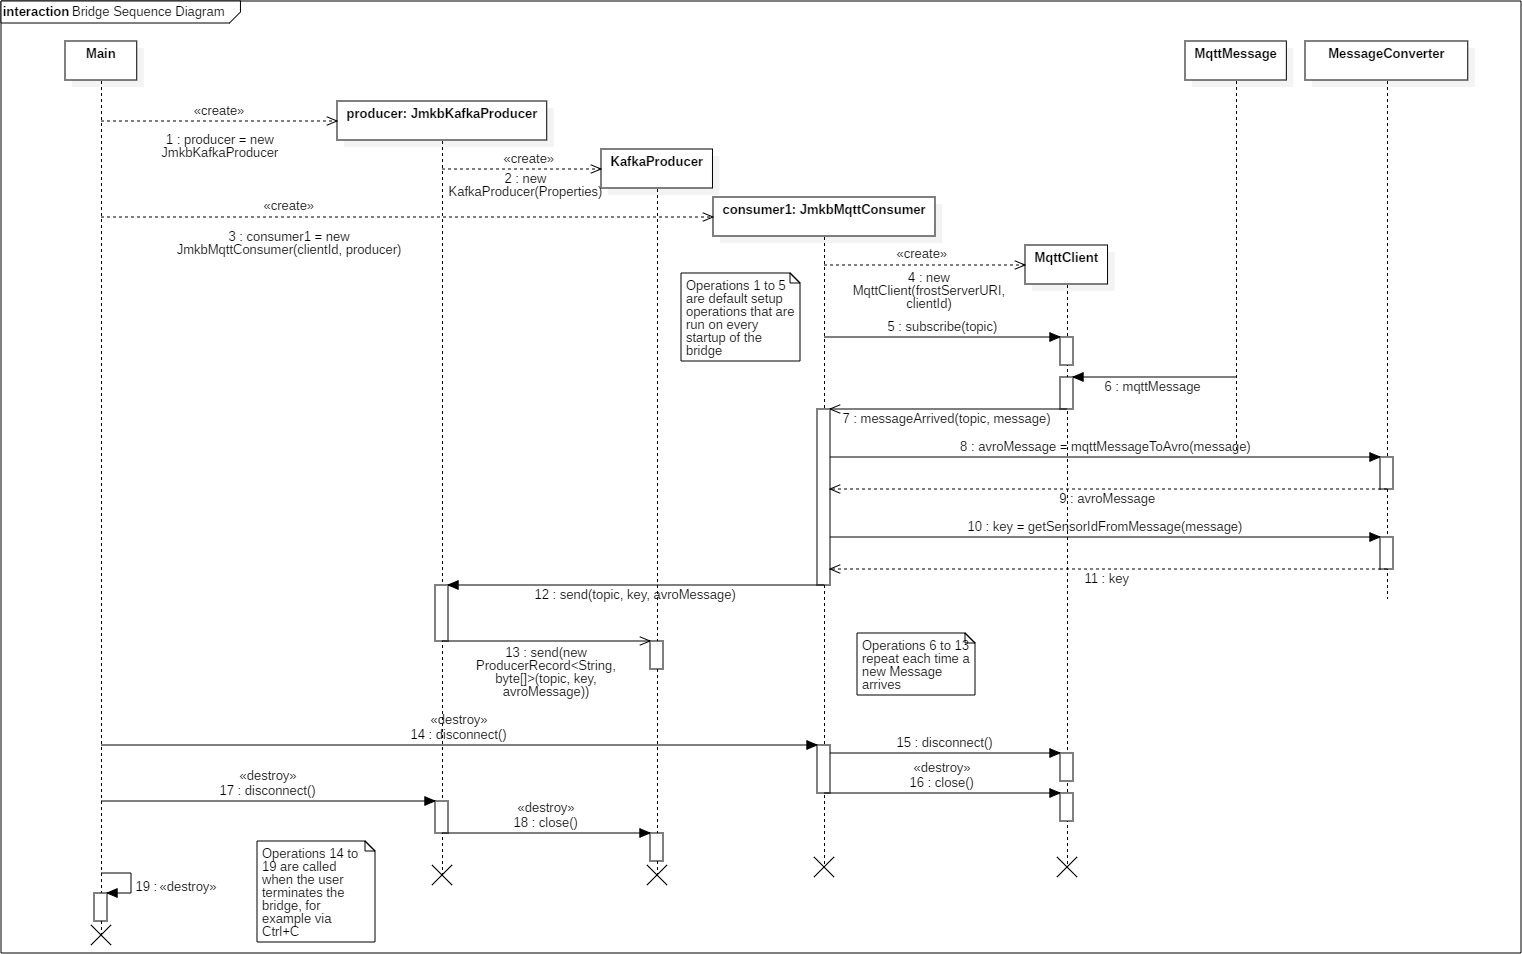
\includegraphics[width=\textheight,angle=90]{images/bridge/BridgeSequenceDiagram.png}
	\caption{Sequenzdiagramm Bridge}
\end{figure}
\newpage

\section{Core}
Beim \texttt{Controller} werden alle Topics, welche von dem MQTT-Producer generierten wurden, in einer Schleife subscribed (abonniert). Dann erzeugt der \texttt{Controller} mit der \texttt{generateOutputtopic} einen neuen Output Topic für eine \texttt{StreamProcessingStrategy}, da dieser ein Output Topic benötigt, um die verarbeiteten Daten abzulagern.
Der \texttt{Controller} konstruiert einen \texttt{TopologyBuilder}, um über diesen die \texttt{StreamProcessingStrategy} ausführen zu können. Mit \texttt{addSource} übergibt der \texttt{Controller} dem \texttt{TopologyBuilder} einen Input Topic, in dem die zu verarbeitenden Daten in einem Kafka Stream enthalten sind.
Der \texttt{Controller} erstellt eine neue \texttt{StreamProcessingStrategy}, die zur Verarbeitung der Inputdaten dienen soll. Der \texttt{Controller} übergibt den \texttt{TopologyBuilder}n mithilfe der \texttt{addProcessor}-Methode diese \texttt{StreamProcessingStrategy}.
Der \texttt{Controller} übergibt den \texttt{TopologyBuilder} mit \texttt{addSink} dem zuvor generierten Output Topic, welcher diesen als Daten-Sink für Daten nutzt, die von der \texttt{StreamProcessingStrategy} verarbeitetet wurden.
Der \texttt{TopologyBuilder} startet nun mit der \texttt{kafkaStreamStart}-Methode die \texttt{StreamProcessingStrategy} und diese beginnt damit durch das Ausführen von \texttt{apply}, aus den Input Topic Daten in den Output Topic zu schreiben, bis der \texttt{TopologyBuilder} \texttt{kafkaStreamClose} aufruft und damit die Verarbeitung stoppt und der \texttt{TopologyBuilder} und die \texttt{StreamProcessingStrategy} zerstört werden.
\begin{figure}[!hbp]
	\centering
	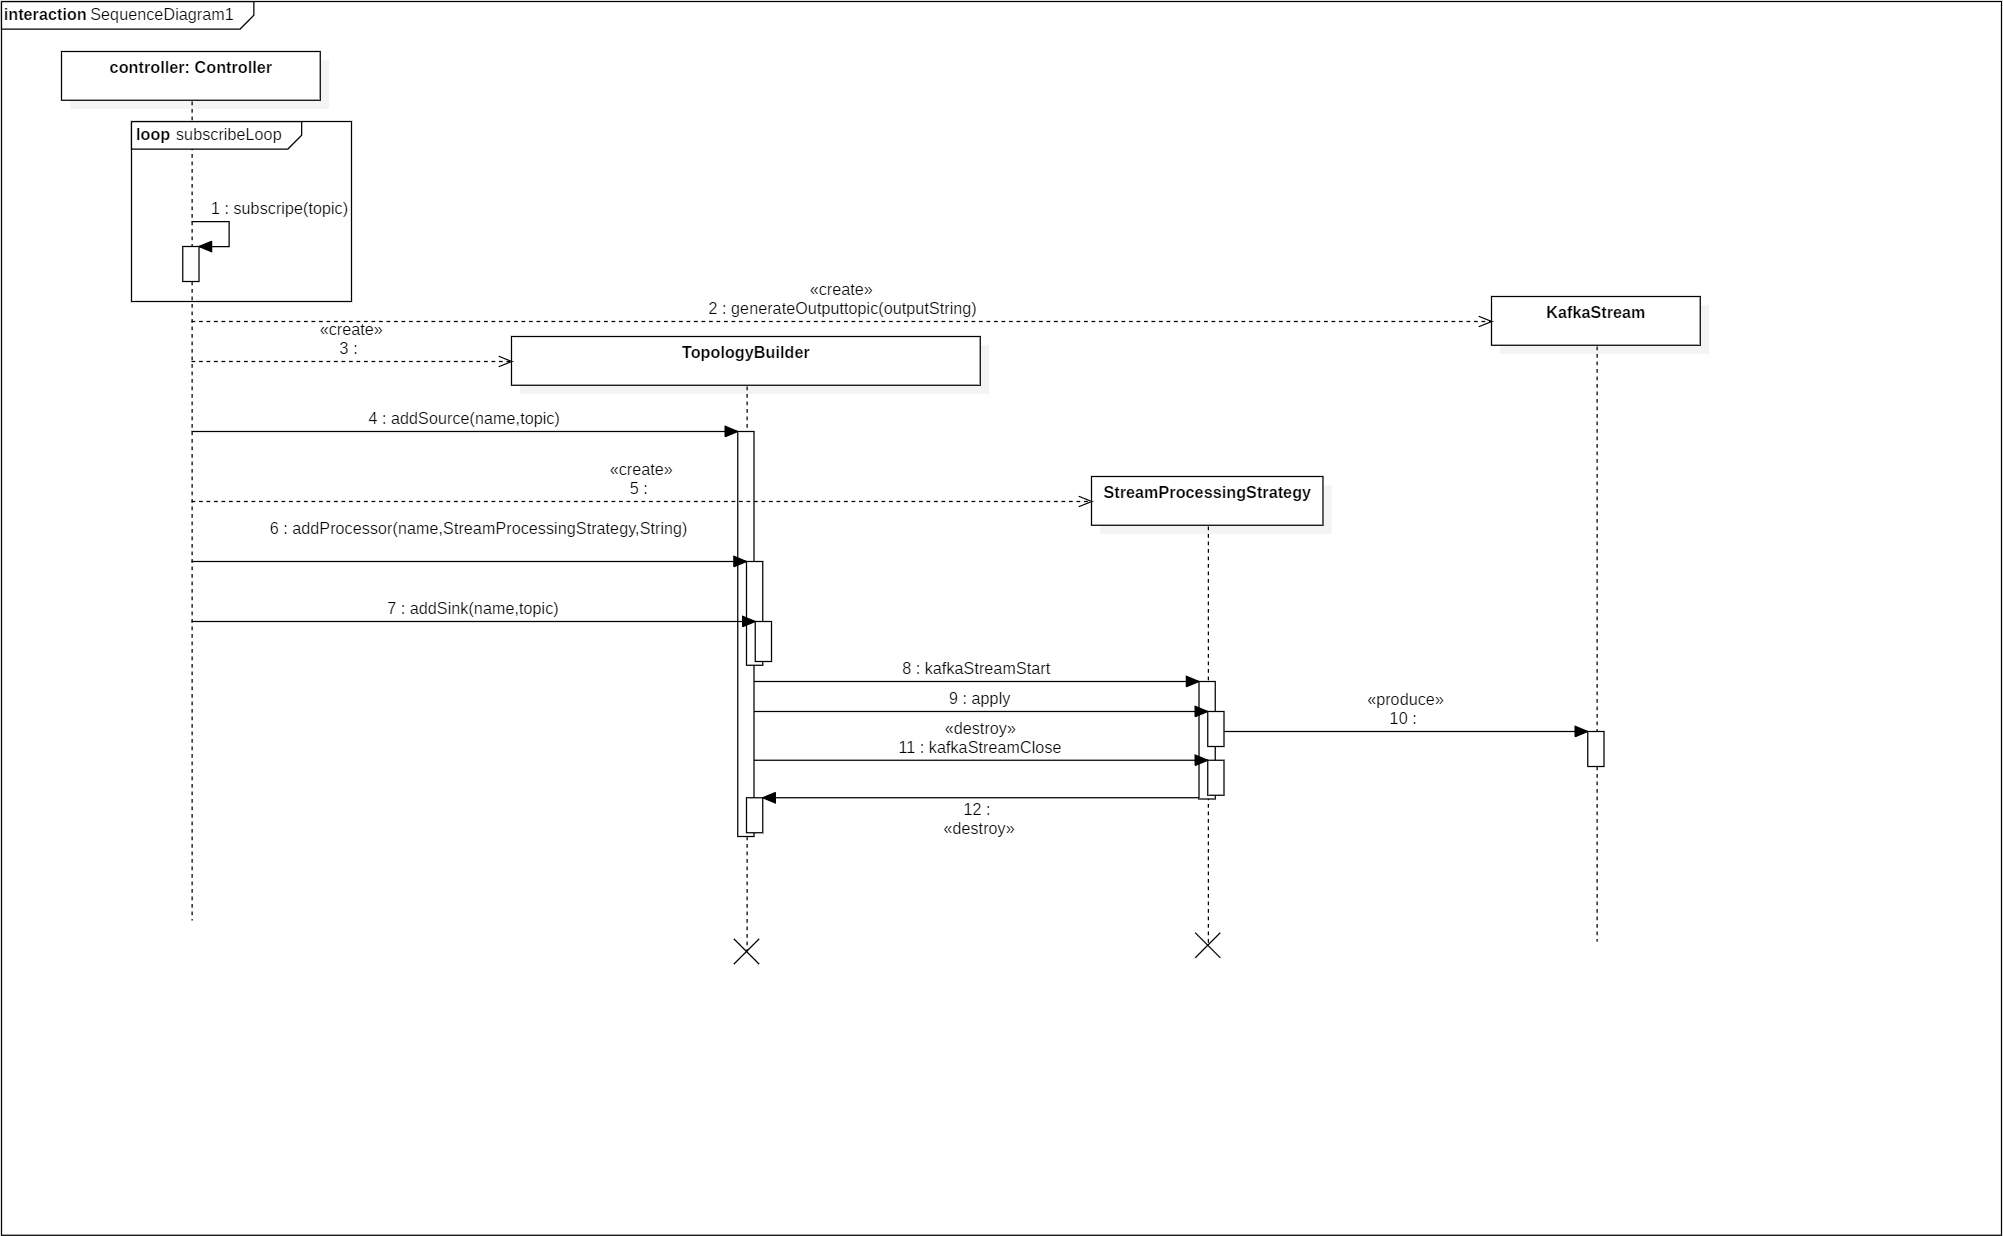
\includegraphics[width=\linewidth]{images/core/CoreSequenceDiagram.png}
	\caption{Sequenzdiagramm Core}
\end{figure}
\newpage

\section{Import}
Bei dem Import wird zuerst in dem Importordner nach Dateien gesucht und danach für jede vorhandene Datei ein separater Importprozess gestartet. Das folgende Sequenzdiagramm stellt diesen Vorgang dar. Hier wird ausschließlich der Import behandelt, wer diesen Anstößt soll nicht Teil des Diagramms sein. \texttt{External} soll hier das Element darstellen, das den Import aufruft. Dazu wird ein \texttt{DataImporter} erstellt und seine Methode \texttt{startImportingFileData} aufgerufen, womit der Importvorgang startet.\\\\
Für jede Datei in dem Importordner wird nun ein \texttt{FrostSender} und ein \texttt{FilePath}, der zum Pfad der Datei passt, erzeugt. Ist dies geschehen wird der \texttt{FileImporter} für diese Datei erschaffen und mit \texttt{addFileData} gestartet. Dazu wird der Pfad und der \texttt{FrostSender} übergeben Aus dem Pfad wird jetzt eine \texttt{FileExtension} generiert, die dazu genutzt wird über den \texttt{ReaderType} eine Instanz einer Implementierung der \texttt{FileReaderStrategy} zu erhalten. Ist die \texttt{FileExtension} nicht bekannt würde es hier zu einer Exception kommen und der Import für diese Datei beendet.\\\\
In diesem Fall wurde als Beispiel eine \texttt{CSVReaderStrategy} genommen. Diese übernimmt den tatsächlichen Import der Daten aus der Datei zum FROST-Server vor. Dazu werden nach und nach einzelne Datensätze aus der Datei ausgelesen und über den \texttt{FrostSender} an den Server gesendet.
\begin{figure}[!hbp]
	\centering
	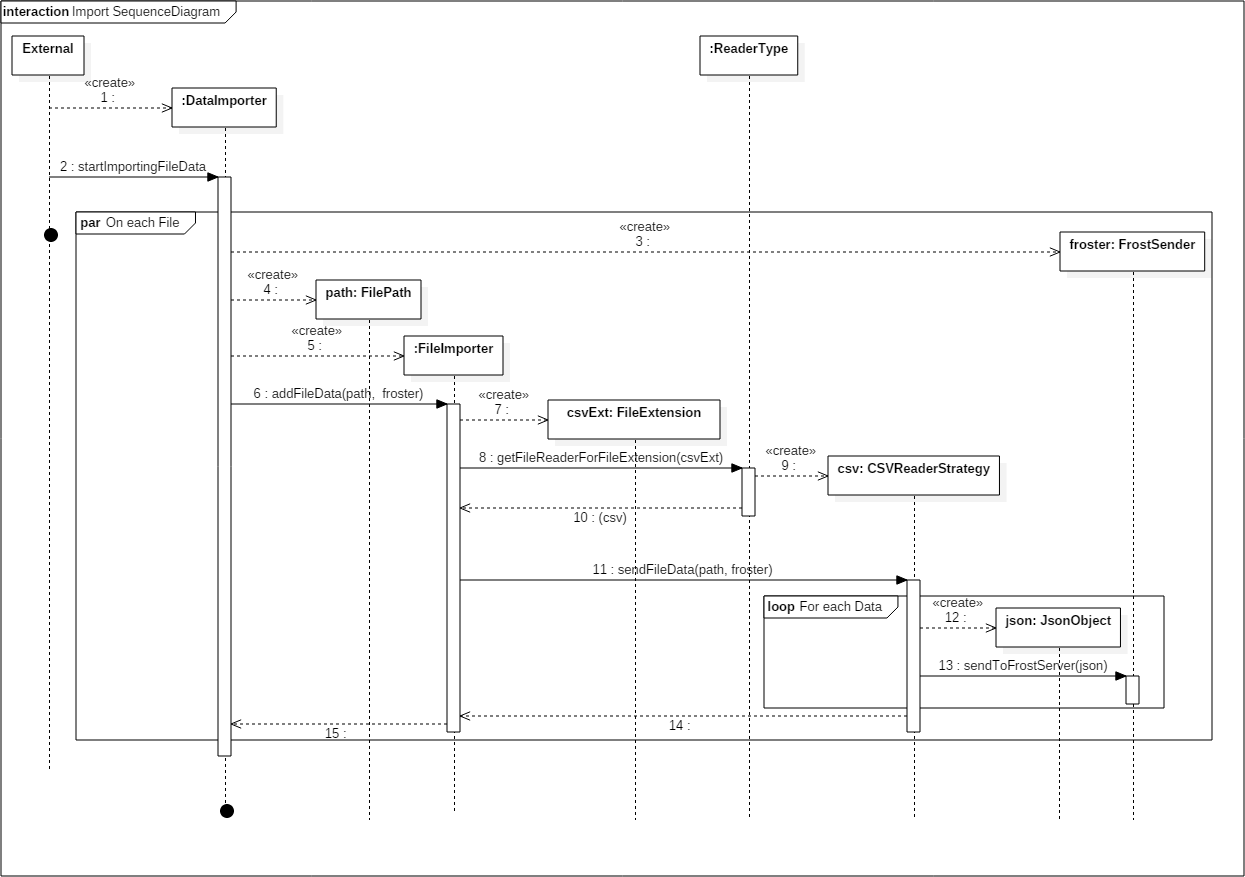
\includegraphics[width=0.9\linewidth]{images/import/ImportSequenceDiagram.png}
	\caption{Sequenzdiagramm Import}
\end{figure}
\newpage

\section{Graphite}
Der Benutzer wählt im Webinterface die Daten aus, die er erhalten will.
Dann erhält das \texttt{Servlet} den Auftrag und leitet dem \texttt{GraphDataTransferController} die Informationen über die Daten weiter, die übertragen werden sollen.
Der \texttt{GraphDataTransferController} erstellt daraufhin einen neuen \texttt{KafkaToGraphiteConsumer}, der ebenfalls diese Informationen erhält und einen \texttt{GraphiteSender} generiert.
Dann wird die Methode \texttt{run} des \texttt{KafkaToGraphiteConsumers} ausgeführt.
Er ruft dann verschiedene Eigenschaften über die \texttt{GraphiteConfig} ab, die benötigt werden um mit Kafka zu kommunizieren.
Weiterhin erzeugt er einen \texttt{KafkaConsumer}, der dann Kafka-Topics abonniert.
Dann prüfen wir ob wir von vorne beginnen wollen.
Danach betreten wir eine Schleife. Hier rufen wir Daten von Kafka ab und speichern sie in einem \texttt{ConsumerRecords} Objekt.
Schlussendlich überprüfen wir, ob die abgerufenen Daten neue Daten enthalten.
Falls ja, senden wir unsere Daten mit Hilfe des \texttt{GraphiteSender}, den wir vorher generiert hatten.
Wenn wir nun die Übertragung der Daten stoppen möchten, müssen wir den \texttt{KafkaConsumer} aufwecken. Dies stoppt die Schleife.
\begin{figure}[!hbp]
	\centering
	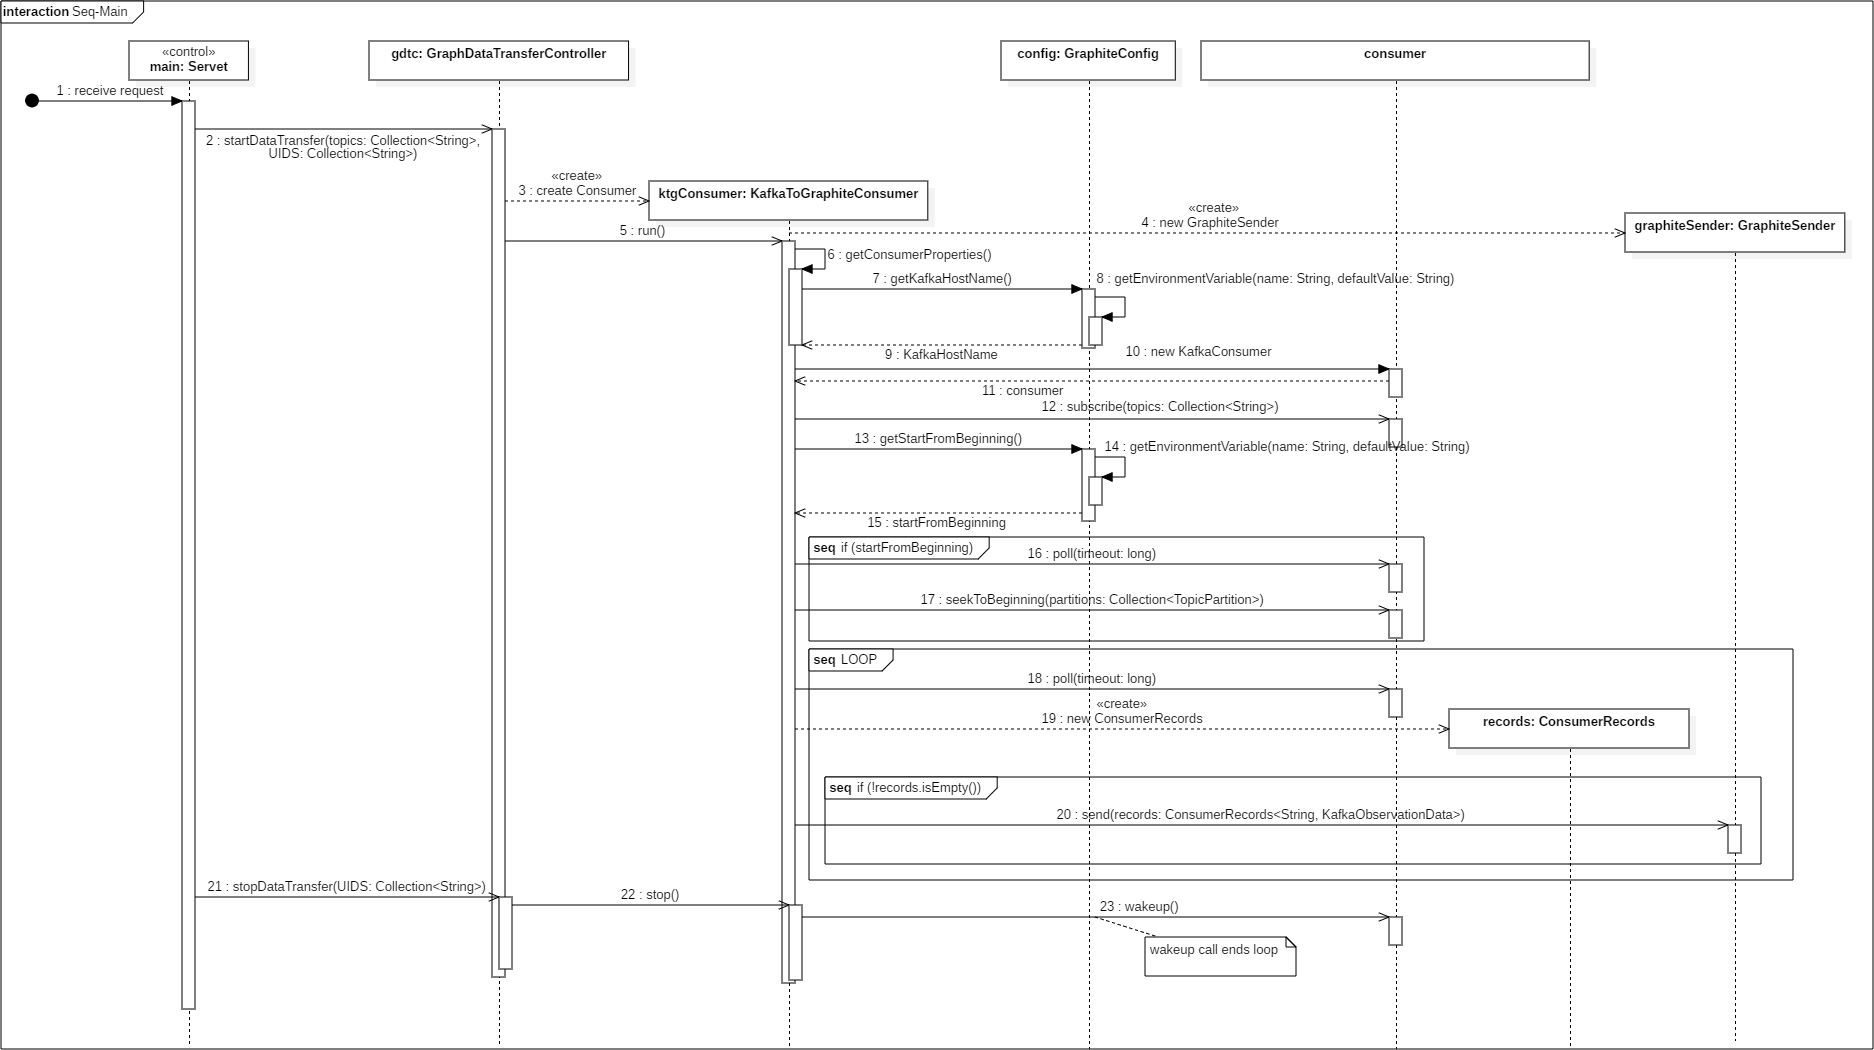
\includegraphics[width=\linewidth]{images/graphite/graphiteMainSequenceDiagram_small.png}
	\caption{Sequenzdiagramm Graphite}
\end{figure}
\newpage
Hier werden die Daten die an Graphite gesendet werden sollen direkt an den \texttt{GraphiteSender} weitergegeben.
Um seine Arbeit zu tun, ruft der \texttt{GraphiteSender} Eigenschaften der \texttt{GraphiteConfig} ab, die notwendig sind, um Daten zu Graphite zu übertragen.
Danach betreten wir die Schleife.
In dieser Schleife, fügt der \texttt{GraphiteSender} jede beobachtete Eigenschaft zur Liste der Daten hinzu, die an Graphite gesendet werden sollen.
Der \texttt{GraphiteSender} tut dies, indem er die Daten zuerst in Metriken konvertiert und dann die Resultate dokumentiert.
Nachdem alle beobachteten Eigenschaften hinzugefügt wurden senden wir die Daten an Graphite.
\begin{figure}[!hbp]
	\centering
	\includegraphics[width=\linewidth]{images/graphite/GraphiteSenderSequenceDiagram.png}
	\caption{Sequenzdiagramm GraphiteSender}
\end{figure}
\newpage

\section{View}
In diesem Funktionsbeispiel der View, wird einem \texttt{MapLayer} einer \texttt{AbstractMap} zunächst ein \texttt{Grid} zugeordnet durch die Methode \texttt{setGrid}. Dann folgt das eigentliche Anzeigen des layers durch die \texttt{displayLayer} Methode. Diese ruft zunächst \texttt{getGrid} um auf die darin enthaltenen \texttt{Cluster} zugreifen zu können durch \texttt{getClusters}. Nun iteriert man über diese und führt für jedes \texttt{Cluster} die Operation \texttt{getTile} aus. Damit hat man Zugriff auf das ihnen zugeordnete \texttt{Tile}. Dies bildet eine graphische Representation und durch die Methode \texttt{display} lässt es sich auf der Karte darstellen. Durch das iterieren über alle \texttt{Cluster} und ihre Visualisierung ergibt sich am ende ein Raster, also die visuelle Representation des \texttt{Grid}.
\begin{figure}[!hbp]
	\centering
	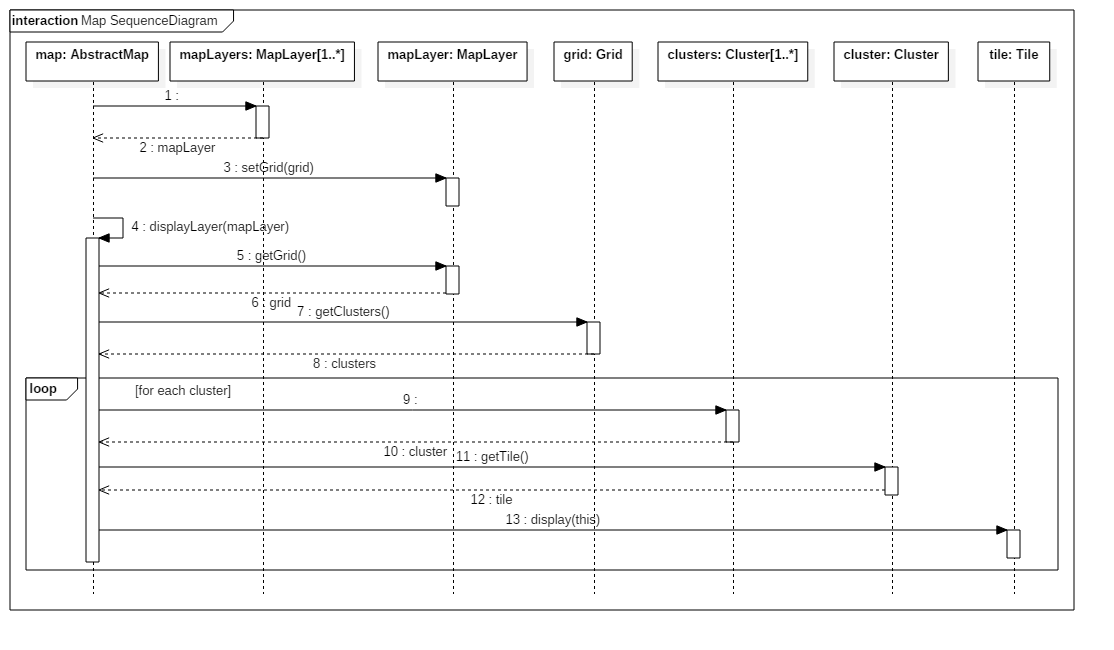
\includegraphics[width=\linewidth]{images/view/ViewSequenceDiagram.png}
	\caption{Sequenzdiagramm View: Anzeigen eines Maplayers}
\end{figure}
\newpage

\section{Export}
Der Export wird in der WebGUI von einem Nutzer angefragt. Die Daten für diesen Export werden an das \texttt{ExportServlet} übertragen, das den tatsächlich Export der Daten in eine Datei verwaltet. Ist diese Datei einmal erstellt, kann diese von dem Nutzer heruntergeladen werden. Dazu mehr in der folgenden Abbildung über den Download. Dieses Sequenzdiagramm zeigt wie der Export der Daten in eine Datei durchgeführt wird.\\\\
Sobald ein Export angestoßen wird, startet das \texttt{ExportServlet} und die Methode \texttt{doGet} wird ausgeführt. Darin werden zuerst die \texttt{ExportProperties} aus der Datei ausgelesen und zu einem Objekt zusammengestellt, das unter anderem eine \texttt{FileExtension} enthält. Danach wird ein \texttt{FileExporter} konstruiert, der in zwei Schritten vorgehen wird, um die Daten zu exportieren.\\\\
Im ersten Schritt, wird durch den Aufruf der \texttt{createFileInformation}-Methode der Export für den späteren Download eindeutig identifiziert, indem ihm eine \texttt{DownloadID} zugewiesen wird. Ein \texttt{AlterableDownloadState} wird erstellt und dessen Methode \texttt{savePersistent} ausgeführt, damit die Information über den Download auch auf dem Server hinterlegt wird, sodass parallel zum Export auch eine Anfrage gesendet werden kann, ob die Datei bereits fertig für den Download ist. Die \texttt{DownloadID} wird dann an den Nutzer zurückgesendet sobald der zweite Teil mit der \texttt{createFile}-Methode des \texttt{FileExporter}s gestartet wurde.\\\\
Im zweiten Schritt, findet dann der tatsächliche Export der Daten in eine Datei statt. Dazu wird zuerst ein \texttt{ExportStreamGenerator} konstruiert, dessen Methode \texttt{createExportStream} einen \texttt{KStream} der gewünschten Daten für den Export erzeugt. Die Gewünschten Daten gehen aus den \texttt{ExportPro-\linebreak perties} hervor. Mit der \texttt{FileExtension} aus den \texttt{ExportProperties} kann jetzt ein \texttt{FileType} generiert werden, über dessen Methode \texttt{getFileWriter} eine neue Instanz einer Implementierung einer \texttt{FileWriterStrategy} zurückgegeben wird. Dazu wird die statische Methode \texttt{getFileWriterFor-\linebreak FileExtension} der Utilityklasse \texttt{FileTypesUtility} verwendet. In diesem Sequenzdiagramm wird als Beispiel eine Instanz der \texttt{CSVWriterStrategy} verwendet.\\\\
Nun wird ein passender neuer Pfad als \texttt{FilePath} erzeugt, um die Datei zu erzeugen. Zur Erzeugung wird die Methode \texttt{saveToFile} einer Implementierung der \texttt{FileWriterStrategy} genutzt. In diesem Fall einer \texttt{CSVWriterStrategy}. Diese Methode benötigt den Zielpfad und den Stream der Daten und erzeugt daraus eine Datei. Ist dies beendet, wird der \texttt{AlterableDownloadState} dazu genutzt, die nötigen Informationen abzuspeichern. Zuerst wird der Pfad der Datei eingegeben und anschließend wird festgelegt, dass die Datei bereit für den Download ist. Zum Schluss wird noch mit \texttt{savePersistent} sichergestellt, dass andere Instanzen eines \texttt{DownloadState} diese Information abrufen können.
\begin{figure}[!hbp]
	\centering
	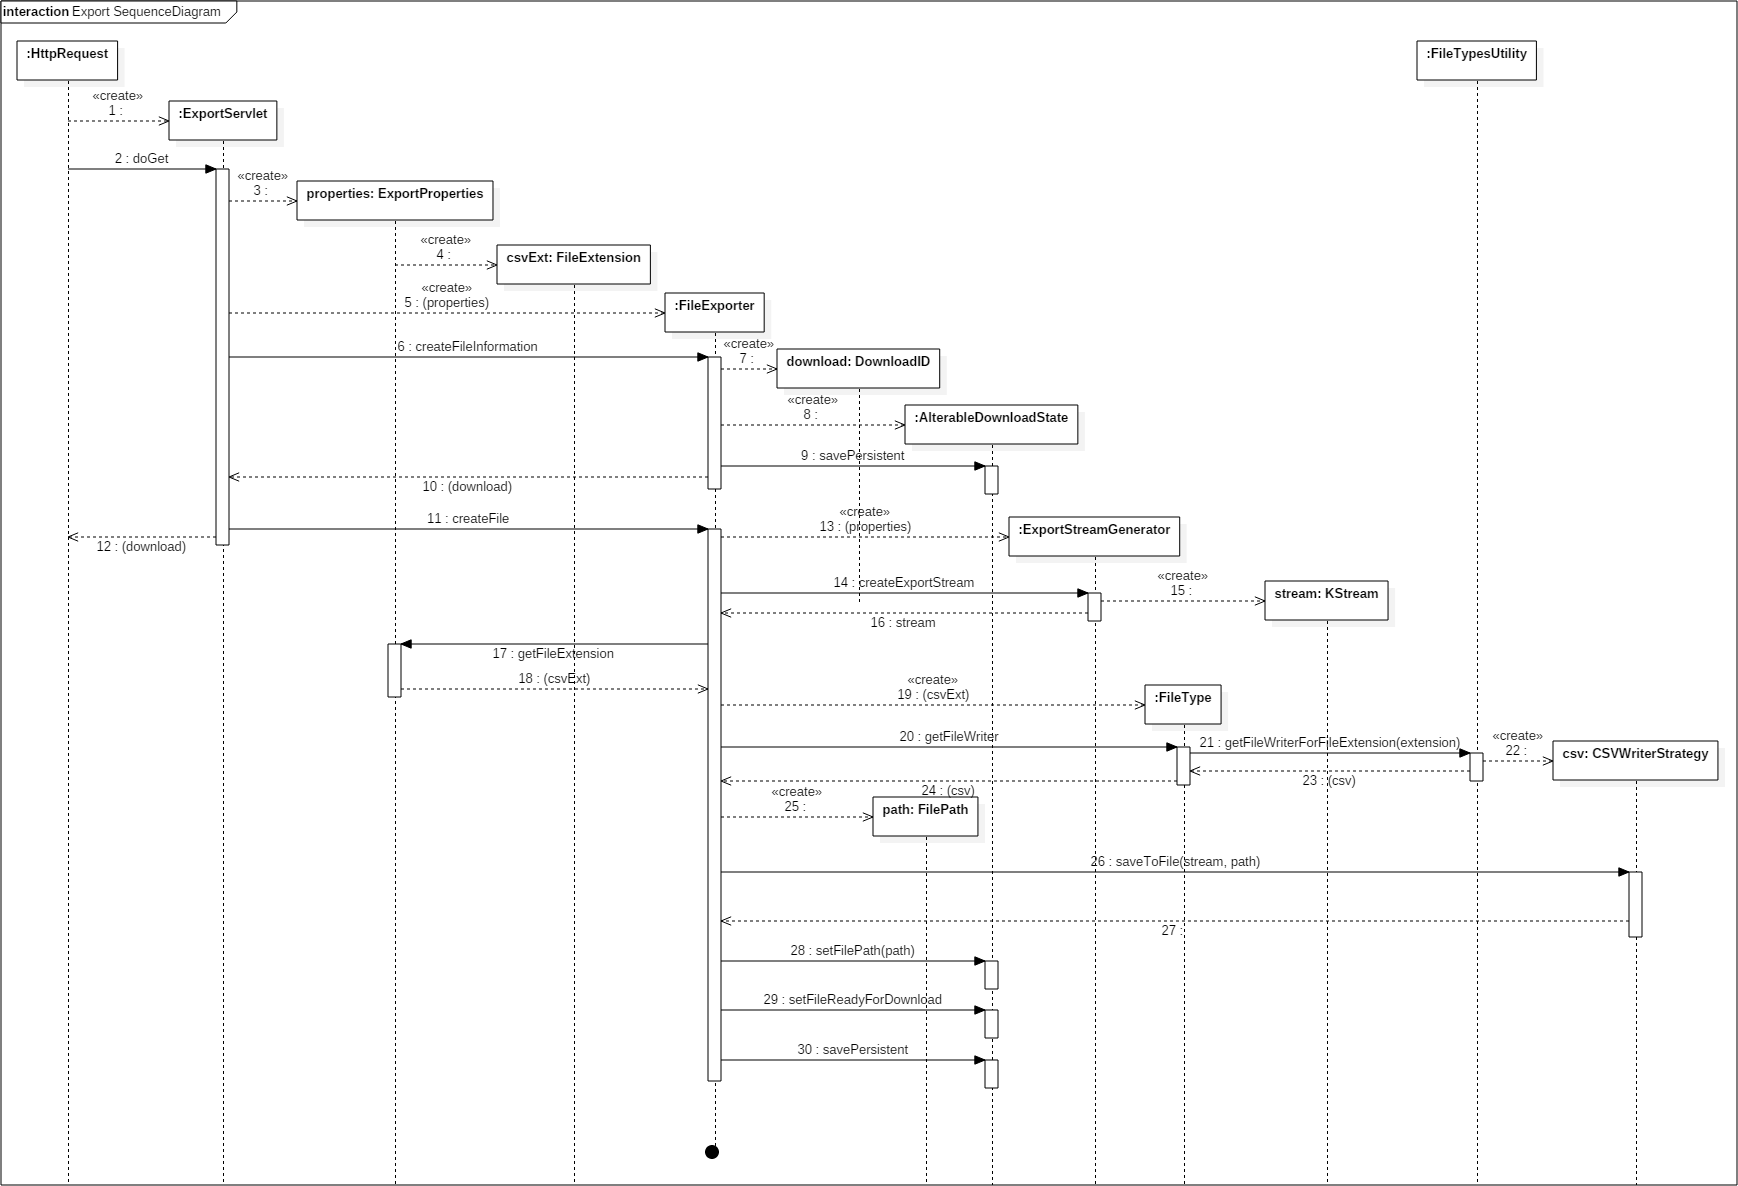
\includegraphics[width=1.25\linewidth,angle=90]{images/export/ExportSequenceDiagram.png}
	\caption{Sequenzdiagramm Export}
\end{figure}
\newpage
Ein Download wird grundsätzlich von einem Nutzer aus einem Browserfenster angefragt. Dazu wird das \texttt{DownloadServlet} benutzt. Diese wird vom Server erstellt sobald eine Anfrage des Nutzer ankommt. Dann wird \texttt{doGet} aufgerufen und das Servlet beginnt mit seiner Aufgabe, die in diesem Sequenzdiagramm dargestellt wird.\\\\
Die Anfrage des Nutzers enthält eine DownloadID, die für eine bestimmte Datei auf dem Server steht. Diese wird benutzt um eine \texttt{DownloadID} Objekt zu erstellen, das dazu dient einen \texttt{DownloadState} zu konstruieren. Dieser holt sich, sobald er erstellt wurde, die Informationen zu dem betreffenden Download. Diese Informationen könnten in einer Datei liegen. Nun wird zuerst geprüft, ob die Datei bereit für den Download ist, dazu dient die Methode \texttt{isFileReadyForDownload}. Ist dies der Fall kann nun mit der \texttt{getFilePath}-Methode nach dem Pfad der Datei gefragt werden. Dieser wird nun vom \texttt{DownloadServlet} genutzt, um die Datei dem Nutzer zu schicken.\\\\
Der Vorgang bei dem \texttt{StatusServlet} ist sehr Ähnlich. Dort geht es darum in Erfahrung zu bringen, ob ein Download bereit ist, um zum Beispiel zu wissen, ob dem Nutzer bereits ein Download-Button gezeigt werden kann. Der einzige Unterschied liegt darin, dass dort nicht nach dem Pfad gesucht wird, sondern gleich das Ergebnis der \texttt{isFileReadyForDownload} zurückgeschickt wird. Aus diesem Grund wurde darauf verzichtet ein separates Sequenzdiagramm dafür zu erstellen.
\begin{figure}[!hbp]
	\centering
	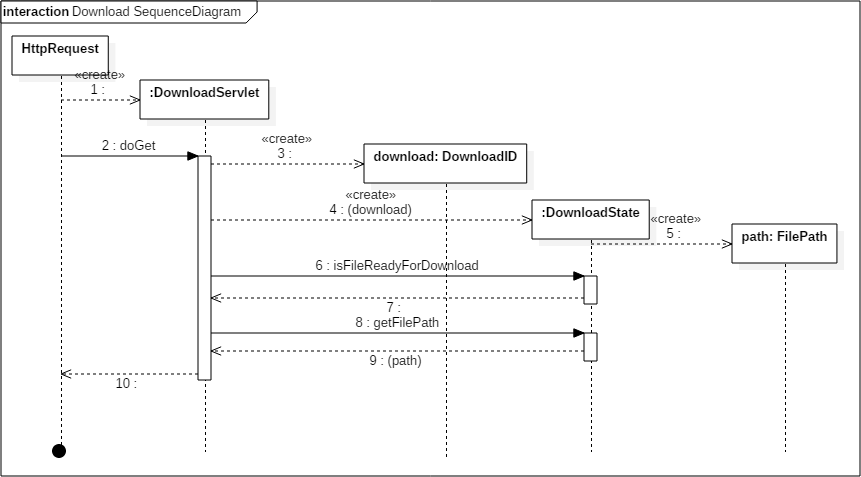
\includegraphics[width=\linewidth]{images/export/DownloadSequenceDiagram.png}
	\caption{Sequenzdiagramm Download}
\end{figure}

	\chapter{Klassenhierarchie}
\subsection*{Classes - Bridge}
{\raggedright
	\hspace{0.0cm} $\bullet$ Bridge.JmkbKafkaProducer {\tiny \refdefined{Bridge.JmkbKafkaProducer}} \\
	\hspace{0.0cm} $\bullet$ Bridge.JmkbMqttConsumer {\tiny \refdefined{Bridge.JmkbMqttConsumer}} \\
	\hspace{0.0cm} $\bullet$ Bridge.MessageConverter {\tiny \refdefined{Bridge.MessageConverter}} \\
	\hspace{0.0cm} $\bullet$ Bridge.PropertiesFileReader {\tiny \refdefined{Bridge.PropertiesFileReader}} \\
	\hspace{0.0cm} $\bullet$ Bridge.SchemaRegistryConnector {\tiny \refdefined{Bridge.SchemaRegistryConnector}} \\
}
\subsection*{Classes - Core}
{\raggedright
	\hspace{0.0cm} $\bullet$ CommandRequestPattern.GetClusterCommand {\tiny \refdefined{CommandRequestPattern.GetClusterCommand}} \\
	\hspace{0.0cm} $\bullet$ CommandRequestPattern.GetSensorCommand {\tiny \refdefined{CommandRequestPattern.GetSensorCommand}} \\
	\hspace{0.0cm} $\bullet$ CommandRequestPattern.GetTileCommand {\tiny \refdefined{CommandRequestPattern.GetTileCommand}} \\
	\hspace{0.0cm} $\bullet$ CommandRequestPattern.Replier {\tiny \refdefined{CommandRequestPattern.Replier}} \\
	\hspace{0.0cm} $\bullet$ CommandRequestPattern.Requestor {\tiny \refdefined{CommandRequestPattern.Requestor}} \\
	\hspace{0.0cm} $\bullet$ ConfigGUI.JFrame {\tiny \refdefined{ConfigGUI.JFrame}} \\
	\hspace{1.0cm} $\bullet$ ConfigGUI.DeleteFrame {\tiny \refdefined{ConfigGUI.DeleteFrame}} \\
	\hspace{1.0cm} $\bullet$ ConfigGUI.MainFrame {\tiny \refdefined{ConfigGUI.MainFrame}} \\
	\hspace{1.0cm} $\bullet$ ConfigGUI.SensorFrame {\tiny \refdefined{ConfigGUI.SensorFrame}} \\
	\hspace{0.0cm} $\bullet$ Controller.ClusterProcessStrategy {\tiny \refdefined{Controller.ClusterProcessStrategy}} \\
	\hspace{0.0cm} $\bullet$ Controller.CombinerProcessStrategy {\tiny \refdefined{Controller.CombinerProcessStrategy}} \\
	\hspace{0.0cm} $\bullet$ Controller.Controller {\tiny \refdefined{Controller.Controller}} \\
	\hspace{0.0cm} $\bullet$ Controller.ExportProcessStrategy {\tiny \refdefined{Controller.ExportProcessStrategy}} \\
	\hspace{0.0cm} $\bullet$ Controller.GraphiteProcessStrategy {\tiny \refdefined{Controller.GraphiteProcessStrategy}} \\
	\hspace{0.0cm} $\bullet$ Controller.TopologyBuilder {\tiny \refdefined{Controller.TopologyBuilder}} \\
	\hspace{0.0cm} $\bullet$ Controller.UncaughtExceptionHandler {\tiny \refdefined{Controller.UncaughtExceptionHandler}} \\
	\hspace{0.0cm} $\bullet$ Properties.PropertiesFile {\tiny \refdefined{Properties.PropertiesFile}} \\
}
\subsection*{Interfaces - Core}
\hspace{0.0cm} $\bullet$ CommandRequestPattern.RequestCommand {\tiny \refdefined{CommandRequestPattern.RequestCommand}} \\
\hspace{0.0cm} $\bullet$ CommandRequestPattern.StreamProcessingStrategy {\tiny \refdefined{CommandRequestPattern.StreamProcessingStrategy}} \\
\hspace{0.0cm} $\bullet$ Properties.PropertiesFileInterface {\tiny \refdefined{Properties.PropertiesFileInterface}} \\
\newpage
\subsection*{Classes - Import}
{\raggedright
	\hspace{0.0cm} $\bullet$ Import.CSVReaderStrategy {\tiny \refdefined{Import.CSVReaderStrategy}} \\
	\hspace{0.0cm} $\bullet$ Import.DataImporter {\tiny \refdefined{Import.DataImporter}} \\
	\hspace{0.0cm} $\bullet$ Import.FileImporter {\tiny \refdefined{Import.FileImporter}} \\
	\hspace{0.0cm} $\bullet$ Import.FrostSender {\tiny \refdefined{Import.FrostSender}} \\
	\hspace{0.0cm} $\bullet$ Import.NetCDFReaderStrategy {\tiny \refdefined{Import.NetCDFReaderStrategy}} \\
	\hspace{0.0cm} $\bullet$ Import.ReaderType {\tiny \refdefined{Import.ReaderType}} \\
}
\subsection*{Interfaces - Import}
\hspace{0.0cm} $\bullet$ Import.FileReaderStrategy {\tiny \refdefined{Import.FileReaderStrategy}} \\
\subsection*{Classes - Database}
{\raggedright
	\hspace{0.0cm} $\bullet$ DatabaseConnection.ClusterID {\tiny \refdefined{DatabaseConnection.ClusterID}} \\
	\hspace{0.0cm} $\bullet$ DatabaseConnection.Facade {\tiny \refdefined{DatabaseConnection.Facade}} \\
	\hspace{0.0cm} $\bullet$ DatabaseConnection.HttpServlet {\tiny \refdefined{DatabaseConnection.HttpServlet}} \\
	\hspace{1.0cm} $\bullet$ DatabaseConnection.GridDataServlet {\tiny \refdefined{DatabaseConnection.GridDataServlet}} \\
	\hspace{1.0cm} $\bullet$ DatabaseConnection.SensorListServlet {\tiny \refdefined{DatabaseConnection.SensorListServlet}} \\
	\hspace{0.0cm} $\bullet$ DatabaseConnection.KafkaToStorageProcessor {\tiny \refdefined{DatabaseConnection.KafkaToStorageProcessor}} \\
	\hspace{0.0cm} $\bullet$ DatabaseConnection.Maintainer {\tiny \refdefined{DatabaseConnection.Maintainer}} \\
	\hspace{1.0cm} $\bullet$ DatabaseConnection.DataMaintainer {\tiny \refdefined{DatabaseConnection.DataMaintainer}} \\
	\hspace{1.0cm} $\bullet$ DatabaseConnection.SensorMaintainer {\tiny \refdefined{DatabaseConnection.SensorMaintainer}} \\
	\hspace{0.0cm} $\bullet$ DatabaseConnection.MaintenanceManager {\tiny \refdefined{DatabaseConnection.MaintenanceManager}} \\
	\hspace{0.0cm} $\bullet$ DatabaseConnection.ZoomLevel {\tiny \refdefined{DatabaseConnection.ZoomLevel}} \\
}
\subsection*{Classes - Graphite}
{\raggedright
	\hspace{0.0cm} $\bullet$ DataTransferControl.Collection {\tiny \refdefined{DataTransferControl.Collection}} \\
	\hspace{0.0cm} $\bullet$ DataTransferControl.Config {\tiny \refdefined{DataTransferControl.Config}} \\
	\hspace{1.0cm} $\bullet$ DataTransferControl.GraphiteConfig {\tiny \refdefined{DataTransferControl.GraphiteConfig}} \\
	\hspace{0.0cm} $\bullet$ DataTransferControl.Consumer {\tiny \refdefined{DataTransferControl.Consumer}} \\
	\hspace{1.0cm} $\bullet$ DataTransferControl.KafkaToGraphiteConsumer {\tiny \refdefined{DataTransferControl.KafkaToGraphiteConsumer}} \\
	\hspace{0.0cm} $\bullet$ DataTransferControl.ConsumerRecord {\tiny \refdefined{DataTransferControl.ConsumerRecord}} \\
	\hspace{0.0cm} $\bullet$ DataTransferControl.ConsumerRecords {\tiny \refdefined{DataTransferControl.ConsumerRecords}} \\
	\hspace{0.0cm} $\bullet$ DataTransferControl.GraphDataTransferController {\tiny \refdefined{DataTransferControl.GraphDataTransferController}} \\
	\hspace{0.0cm} $\bullet$ DataTransferControl.KafkaConsumer {\tiny \refdefined{DataTransferControl.KafkaConsumer}} \\
	\hspace{0.0cm} $\bullet$ DataTransferControl.Properties {\tiny \refdefined{DataTransferControl.Properties}} \\
	\hspace{0.0cm} $\bullet$ DataTransferControl.Sender {\tiny \refdefined{DataTransferControl.Sender}} \\
	\hspace{1.0cm} $\bullet$ DataTransferControl.GraphiteSender {\tiny \refdefined{DataTransferControl.GraphiteSender}} \\
	\hspace{0.0cm} $\bullet$ DataTransferControl.SerializationDeserialization.KafkaObservationData {\tiny \refdefined{DataTransferControl.SerializationDeserialization.KafkaObservationData}} \\
	\hspace{0.0cm} $\bullet$ DataTransferControl.SerializationDeserialization.ObservationDataDeserializer {\tiny \refdefined{DataTransferControl.SerializationDeserialization.ObservationDataDeserializer}} \\
	\hspace{0.0cm} $\bullet$ DataTransferControl.Servet {\tiny \refdefined{DataTransferControl.Servet}} \\
}
\subsection*{Classes - View}
{\raggedright
	\hspace{0.0cm} $\bullet$ Grid.Cluster {\tiny \refdefined{Grid.Cluster}} \\
	\hspace{0.0cm} $\bullet$ Grid.Dimension {\tiny \refdefined{Grid.Dimension}} \\
	\hspace{0.0cm} $\bullet$ Grid.Grid {\tiny \refdefined{Grid.Grid}} \\
	\hspace{0.0cm} $\bullet$ Grid.Image {\tiny \refdefined{Grid.Image}} \\
	\hspace{0.0cm} $\bullet$ Grid.Tile {\tiny \refdefined{Grid.Tile}} \\
	\hspace{1.0cm} $\bullet$ Grid.ImageTile {\tiny \refdefined{Grid.ImageTile}} \\
	\hspace{1.0cm} $\bullet$ Grid.ShapeTile {\tiny \refdefined{Grid.ShapeTile}} \\
	\hspace{0.0cm} $\bullet$ View.AbstractView {\tiny \refdefined{View.AbstractView}} \\
	\hspace{1.0cm} $\bullet$ View.View {\tiny \refdefined{View.View}} \\
	\hspace{0.0cm} $\bullet$ View.AbstractViewFactory {\tiny \refdefined{View.AbstractViewFactory}} \\
	\hspace{1.0cm} $\bullet$ View.ViewFactory {\tiny \refdefined{View.ViewFactory}} \\
	\hspace{0.0cm} $\bullet$ View.Graph.GraphDisplayType {\tiny \refdefined{View.Graph.GraphDisplayType}} \\
	\hspace{0.0cm} $\bullet$ View.Map.MapLayer {\tiny \refdefined{View.Map.MapLayer}} \\
	\hspace{0.0cm} $\bullet$ View.Map.TileType {\tiny \refdefined{View.Map.TileType}} \\
	\hspace{0.0cm} $\bullet$ View.SensorOption.ObservedProperty {\tiny \refdefined{View.SensorOption.ObservedProperty}} \\
	\hspace{0.0cm} $\bullet$ View.TimeOption.RefreshConfiguration {\tiny \refdefined{View.TimeOption.RefreshConfiguration}} \\
	\hspace{0.0cm} $\bullet$ View.TimeOption.RefreshContext {\tiny \refdefined{View.TimeOption.RefreshContext}} \\
	\hspace{0.0cm} $\bullet$ View.TimeOption.RefreshState {\tiny \refdefined{View.TimeOption.RefreshState}} \\
	\hspace{1.0cm} $\bullet$ View.TimeOption.HistoricalRefreshState {\tiny \refdefined{View.TimeOption.HistoricalRefreshState}} \\
	\hspace{1.0cm} $\bullet$ View.TimeOption.LiveRefreshState {\tiny \refdefined{View.TimeOption.LiveRefreshState}} \\
	\hspace{1.0cm} $\bullet$ View.TimeOption.LoopRefreshState {\tiny \refdefined{View.TimeOption.LoopRefreshState}} \\
	\hspace{0.0cm} $\bullet$ View.Util.Date {\tiny \refdefined{View.Util.Date}} \\
	\hspace{0.0cm} $\bullet$ View.Util.Identifier {\tiny \refdefined{View.Util.Identifier}} \\
	\hspace{1.0cm} $\bullet$ View.Util.ClusterID {\tiny \refdefined{View.Util.ClusterID}} \\
	\hspace{1.0cm} $\bullet$ View.Util.SensorID {\tiny \refdefined{View.Util.SensorID}} \\
	\hspace{0.0cm} $\bullet$ View.Util.Point {\tiny \refdefined{View.Util.Point}} \\
	\hspace{0.0cm} $\bullet$ View.Util.TimeFrame {\tiny \refdefined{View.Util.TimeFrame}} \\
	\hspace{0.0cm} $\bullet$ View.ViewComponent {\tiny \refdefined{View.ViewComponent}} \\
	\hspace{0.0cm} $\bullet$ View.ViewManager {\tiny \refdefined{View.ViewManager}} \\
	\hspace{0.0cm} $\bullet$ ViewComponent {\tiny } \\
	\hspace{1.0cm} $\bullet$ View.ExportOption.AbstractExportOptionPanel {\tiny \refdefined{View.ExportOption.AbstractExportOptionPanel}} \\
	\hspace{2.0cm} $\bullet$ View.ExportOption.ExportOptionPanel {\tiny \refdefined{View.ExportOption.ExportOptionPanel}} \\
	\hspace{1.0cm} $\bullet$ View.Graph.AbstractGraph {\tiny \refdefined{View.Graph.AbstractGraph}} \\
	\hspace{2.0cm} $\bullet$ View.Graph.GraphiteGraph {\tiny \refdefined{View.Graph.GraphiteGraph}} \\
	\hspace{1.0cm} $\bullet$ View.Graph.AbstractGraphOptionPanel {\tiny \refdefined{View.Graph.AbstractGraphOptionPanel}} \\
	\hspace{2.0cm} $\bullet$ View.Graph.GraphOptionPanel {\tiny \refdefined{View.Graph.GraphOptionPanel}} \\
	\hspace{1.0cm} $\bullet$ View.Map.AbstractMap {\tiny \refdefined{View.Map.AbstractMap}} \\
	\hspace{2.0cm} $\bullet$ View.Map.LeafletMap {\tiny \refdefined{View.Map.LeafletMap}} \\
	\hspace{1.0cm} $\bullet$ View.Map.AbstractMapOptionPanel {\tiny \refdefined{View.Map.AbstractMapOptionPanel}} \\
	\hspace{2.0cm} $\bullet$ View.Map.MapOptionPanel {\tiny \refdefined{View.Map.MapOptionPanel}} \\
	\hspace{1.0cm} $\bullet$ View.SensorOption.AbstractSensorOptionPanel {\tiny \refdefined{View.SensorOption.AbstractSensorOptionPanel}} \\
	\hspace{2.0cm} $\bullet$ View.SensorOption.SensorOptionPanel {\tiny \refdefined{View.SensorOption.SensorOptionPanel}} \\
	\hspace{1.0cm} $\bullet$ View.SensorTable.AbstractSensorTable {\tiny \refdefined{View.SensorTable.AbstractSensorTable}} \\
	\hspace{2.0cm} $\bullet$ View.SensorTable.SensorTable {\tiny \refdefined{View.SensorTable.SensorTable}} \\
	\hspace{1.0cm} $\bullet$ View.TimeOption.AbstractTimeOptionPanel {\tiny \refdefined{View.TimeOption.AbstractTimeOptionPanel}} \\
	\hspace{2.0cm} $\bullet$ View.TimeOption.TimeOptionPanel {\tiny \refdefined{View.TimeOption.TimeOptionPanel}} \\
}
\subsection*{Interfaces - View}
\hspace{0.0cm} $\bullet$ View.Graph.GraphOptionPanelObserver {\tiny \refdefined{View.Graph.GraphOptionPanelObserver}} \\
\hspace{0.0cm} $\bullet$ View.Map.MapObserver {\tiny \refdefined{View.Map.MapObserver}} \\
\hspace{0.0cm} $\bullet$ View.Map.MapOptionPanelObserver {\tiny \refdefined{View.Map.MapOptionPanelObserver}} \\
\hspace{0.0cm} $\bullet$ View.SensorOption.SensorOptionPanelObserver {\tiny \refdefined{View.SensorOption.SensorOptionPanelObserver}} \\
\hspace{0.0cm} $\bullet$ View.TimeOption.TimeOptionPanelObserver {\tiny \refdefined{View.TimeOption.TimeOptionPanelObserver}} \\
\subsection*{Classes - Export}
{\raggedright
	\hspace{0.0cm} $\bullet$ Download.DownloadID {\tiny \refdefined{Download.DownloadID}} \\
	\hspace{0.0cm} $\bullet$ Download.DownloadState {\tiny \refdefined{Download.DownloadState}} \\
	\hspace{1.0cm} $\bullet$ Download.AlterableDownloadState {\tiny \refdefined{Download.AlterableDownloadState}} \\
	\hspace{0.0cm} $\bullet$ Export.AbstractExporter {\tiny \refdefined{Export.AbstractExporter}} \\
	\hspace{1.0cm} $\bullet$ Export.FileExporter {\tiny \refdefined{Export.FileExporter}} \\
	\hspace{0.0cm} $\bullet$ Export.CSVWriterStrategy {\tiny \refdefined{Export.CSVWriterStrategy}} \\
	\hspace{0.0cm} $\bullet$ Export.ExportProperties {\tiny \refdefined{Export.ExportProperties}} \\
	\hspace{0.0cm} $\bullet$ Export.ExportStreamGenerator {\tiny \refdefined{Export.ExportStreamGenerator}} \\
	\hspace{0.0cm} $\bullet$ Export.FileExtension {\tiny \refdefined{Export.FileExtension}} \\
	\hspace{0.0cm} $\bullet$ Export.FileType {\tiny \refdefined{Export.FileType}} \\
	\hspace{0.0cm} $\bullet$ Export.FileTypesUtility {\tiny \refdefined{Export.FileTypesUtility}} \\
	\hspace{0.0cm} $\bullet$ Export.NetCDFWriterStrategy {\tiny \refdefined{Export.NetCDFWriterStrategy}} \\
	\hspace{0.0cm} $\bullet$ ExportDownloadCommunication.HttpServlet {\tiny \refdefined{ExportDownloadCommunication.HttpServlet}} \\
	\hspace{1.0cm} $\bullet$ ExportDownloadCommunication.DownloadServlet {\tiny \refdefined{ExportDownloadCommunication.DownloadServlet}} \\
	\hspace{1.0cm} $\bullet$ ExportDownloadCommunication.ExportServlet {\tiny \refdefined{ExportDownloadCommunication.ExportServlet}} \\
	\hspace{1.0cm} $\bullet$ ExportDownloadCommunication.FileExtensionServlet {\tiny \refdefined{ExportDownloadCommunication.FileExtensionServlet}} \\
	\hspace{1.0cm} $\bullet$ ExportDownloadCommunication.StatusServlet {\tiny \refdefined{ExportDownloadCommunication.StatusServlet}} \\
}
\subsection*{Interfaces - Export}
\hspace{0.0cm} $\bullet$ Export.FileWriterStrategy {\tiny \refdefined{Export.FileWriterStrategy}} \\
	\chapter{Klassendiagramme}
\section*{Class Hierarchy}{
\thispagestyle{empty}
\markboth{Class Hierarchy}{Class Hierarchy}
\addcontentsline{toc}{section}{Class Hierarchy}
\subsection*{Classes}
{\raggedright
\hspace{0.0cm} $\bullet$ java.lang.Object {\tiny \refdefined{java.lang.Object}} \\
\hspace{1.0cm} $\bullet$ Bridge.JmkbKafkaProducer {\tiny \refdefined{Bridge.JmkbKafkaProducer}} \\
\hspace{1.0cm} $\bullet$ Bridge.JmkbMqttConsumer {\tiny \refdefined{Bridge.JmkbMqttConsumer}} \\
\hspace{1.0cm} $\bullet$ Bridge.MessageConverter {\tiny \refdefined{Bridge.MessageConverter}} \\
\hspace{1.0cm} $\bullet$ Bridge.PropertiesFileReader {\tiny \refdefined{Bridge.PropertiesFileReader}} \\
\hspace{1.0cm} $\bullet$ Bridge.SchemaRegistryConnector {\tiny \refdefined{Bridge.SchemaRegistryConnector}} \\
}
}
\section{Package Bridge}{
\label{Bridge}\hypertarget{Bridge}{}
\hskip -.05in
\hbox to \hsize{\textit{ Package Contents\hfil Page}}
\vskip .13in
\hbox{{\bf  Classes}}
\entityintro{JmkbKafkaProducer}{Bridge.JmkbKafkaProducer}{This class creates a Kafka producer using defined settings and publishes records to the Kafka Cluster.}
\entityintro{JmkbMqttConsumer}{Bridge.JmkbMqttConsumer}{This class serves as an MqttClient that consumes messages from the specified FROST-Server address.}
\entityintro{MessageConverter}{Bridge.MessageConverter}{This convenience class provides static methods to convert a given message to another format.}
\entityintro{PropertiesFileReader}{Bridge.PropertiesFileReader}{A class that reads properties from the configuration file (jmkb.properties) and provides a method for getting a property by key.}
\entityintro{SchemaRegistryConnector}{Bridge.SchemaRegistryConnector}{Convenience class which provides methods for interacting with the schema registry.}
\vskip .1in
\vskip .1in
\subsection{\label{Bridge.JmkbKafkaProducer}Class JmkbKafkaProducer}{
\hypertarget{Bridge.JmkbKafkaProducer}{}\vskip .1in 
This class creates a Kafka producer using defined settings and publishes records to the Kafka Cluster.\vskip .1in 
\subsubsection{Declaration}{
\begin{lstlisting}[frame=none]
public class JmkbKafkaProducer
 extends java.lang.Object\end{lstlisting}
\subsubsection{Constructor summary}{
\begin{verse}
\hyperlink{Bridge.JmkbKafkaProducer()}{{\bf JmkbKafkaProducer()}} Default constructor\\
\end{verse}
}
\subsubsection{Method summary}{
\begin{verse}
\hyperlink{Bridge.JmkbKafkaProducer.disconnect()}{{\bf disconnect()}} Disconnects this Kafka producer from the Kafka Cluster and closes the producer.\\
\hyperlink{Bridge.JmkbKafkaProducer.send(java.lang.String, byte[])}{{\bf send(String, byte\lbrack \rbrack )}} Asynchronously sends a record to the topic.\\
\end{verse}
}
\subsubsection{Constructors}{
\vskip -2em
\begin{itemize}
\item{ 
\index{JmkbKafkaProducer()}
\hypertarget{Bridge.JmkbKafkaProducer()}{{\bf  JmkbKafkaProducer}\\}
\begin{lstlisting}[frame=none]
public JmkbKafkaProducer()\end{lstlisting} %end signature
\begin{itemize}
\item{
{\bf  Description}

Default constructor
}
\end{itemize}
}%end item
\end{itemize}
}
\subsubsection{Methods}{
\vskip -2em
\begin{itemize}
\item{ 
\index{disconnect()}
\hypertarget{Bridge.JmkbKafkaProducer.disconnect()}{{\bf  disconnect}\\}
\begin{lstlisting}[frame=none]
public void disconnect()\end{lstlisting} %end signature
\begin{itemize}
\item{
{\bf  Description}

Disconnects this Kafka producer from the Kafka Cluster and closes the producer.
}
\end{itemize}
}%end item
\item{ 
\index{send(String, byte\lbrack \rbrack )}
\hypertarget{Bridge.JmkbKafkaProducer.send(java.lang.String, byte[])}{{\bf  send}\\}
\begin{lstlisting}[frame=none]
public void send(java.lang.String topic,byte[] avroMessage)\end{lstlisting} %end signature
\begin{itemize}
\item{
{\bf  Description}

Asynchronously sends a record to the topic.
}
\item{
{\bf  Parameters}
  \begin{itemize}
   \item{
\texttt{topic} -- The topic.}
   \item{
\texttt{avroMessage} -- The message to send.}
  \end{itemize}
}%end item
\end{itemize}
}%end item
\end{itemize}
}
}
\subsection{\label{Bridge.JmkbMqttConsumer}Class JmkbMqttConsumer}{
\hypertarget{Bridge.JmkbMqttConsumer}{}\vskip .1in 
This class serves as an MqttClient that consumes messages from the specified FROST-Server address. On message arrival, it will initiate the conversion of the message to a desired format via MqttMessageConverter and supply the converted message to a JmkbKafkaProducer. An instance of this class should be destroyed with a call to the disconnect() method.\vskip .1in 
\subsubsection{Declaration}{
\begin{lstlisting}[frame=none]
public class JmkbMqttConsumer
 extends java.lang.Object\end{lstlisting}
\subsubsection{Constructor summary}{
\begin{verse}
\hyperlink{Bridge.JmkbMqttConsumer()}{{\bf JmkbMqttConsumer()}} Default constructor\\
\end{verse}
}
\subsubsection{Method summary}{
\begin{verse}
\hyperlink{Bridge.JmkbMqttConsumer.connectionLost(java.lang.Throwable)}{{\bf connectionLost(Throwable)}} This method is called when the connection to the server is lost.\\
\hyperlink{Bridge.JmkbMqttConsumer.deliveryComplete(IMqttDeliveryToken)}{{\bf deliveryComplete(IMqttDeliveryToken)}} Called when delivery for a message has been completed, and all acknowledgments have been received.\\
\hyperlink{Bridge.JmkbMqttConsumer.disconnect()}{{\bf disconnect()}} Disconnects client from MQTT and closes the client.\\
\hyperlink{Bridge.JmkbMqttConsumer.JmkbMqttConsumer(java.lang.String, Bridge.JmkbKafkaProducer)}{{\bf JmkbMqttConsumer(String, JmkbKafkaProducer)}} This constructor for this class.\\
\hyperlink{Bridge.JmkbMqttConsumer.messageArrived(java.lang.String, MqttMessage)}{{\bf messageArrived(String, MqttMessage)}} This method is called when a message arrives from the server.\\
\end{verse}
}
\subsubsection{Constructors}{
\vskip -2em
\begin{itemize}
\item{ 
\index{JmkbMqttConsumer()}
\hypertarget{Bridge.JmkbMqttConsumer()}{{\bf  JmkbMqttConsumer}\\}
\begin{lstlisting}[frame=none]
public JmkbMqttConsumer()\end{lstlisting} %end signature
\begin{itemize}
\item{
{\bf  Description}

Default constructor
}
\end{itemize}
}%end item
\end{itemize}
}
\subsubsection{Methods}{
\vskip -2em
\begin{itemize}
\item{ 
\index{connectionLost(Throwable)}
\hypertarget{Bridge.JmkbMqttConsumer.connectionLost(java.lang.Throwable)}{{\bf  connectionLost}\\}
\begin{lstlisting}[frame=none]
public void connectionLost(java.lang.Throwable cause)\end{lstlisting} %end signature
\begin{itemize}
\item{
{\bf  Description}

This method is called when the connection to the server is lost.
}
\item{
{\bf  Parameters}
  \begin{itemize}
   \item{
\texttt{cause} -- the reason behind the loss of connection.}
  \end{itemize}
}%end item
\end{itemize}
}%end item
\item{ 
\index{deliveryComplete(IMqttDeliveryToken)}
\hypertarget{Bridge.JmkbMqttConsumer.deliveryComplete(IMqttDeliveryToken)}{{\bf  deliveryComplete}\\}
\begin{lstlisting}[frame=none]
public void deliveryComplete(IMqttDeliveryToken token)\end{lstlisting} %end signature
\begin{itemize}
\item{
{\bf  Description}

Called when delivery for a message has been completed, and all acknowledgments have been received. In this implementation of this method, nothing happens.
}
\item{
{\bf  Parameters}
  \begin{itemize}
   \item{
\texttt{token} -- the delivery token associated with the message.}
  \end{itemize}
}%end item
\end{itemize}
}%end item
\item{ 
\index{disconnect()}
\hypertarget{Bridge.JmkbMqttConsumer.disconnect()}{{\bf  disconnect}\\}
\begin{lstlisting}[frame=none]
public void disconnect()\end{lstlisting} %end signature
\begin{itemize}
\item{
{\bf  Description}

Disconnects client from MQTT and closes the client.
}
\end{itemize}
}%end item
\item{ 
\index{JmkbMqttConsumer(String, JmkbKafkaProducer)}
\hypertarget{Bridge.JmkbMqttConsumer.JmkbMqttConsumer(java.lang.String, Bridge.JmkbKafkaProducer)}{{\bf  JmkbMqttConsumer}\\}
\begin{lstlisting}[frame=none]
public void JmkbMqttConsumer(java.lang.String clientId,JmkbKafkaProducer producer)\end{lstlisting} %end signature
\begin{itemize}
\item{
{\bf  Description}

This constructor for this class. Creates a new MqttClient and subscribes to the topics specified in the SensorThings API standard. A unique identifier and a JmkbKafkaProducer should be supplied.
}
\item{
{\bf  Parameters}
  \begin{itemize}
   \item{
\texttt{clientId} -- The unique identifier for the MqttClient.}
   \item{
\texttt{producer} -- A JmkbKafkaProducer.}
  \end{itemize}
}%end item
\end{itemize}
}%end item
\item{ 
\index{messageArrived(String, MqttMessage)}
\hypertarget{Bridge.JmkbMqttConsumer.messageArrived(java.lang.String, MqttMessage)}{{\bf  messageArrived}\\}
\begin{lstlisting}[frame=none]
public void messageArrived(java.lang.String topic,MqttMessage message)\end{lstlisting} %end signature
\begin{itemize}
\item{
{\bf  Description}

This method is called when a message arrives from the server. This method is invoked synchronously by the MQTT client. An acknowledgment is not sent back to the server until this method returns cleanly. Any additional messages which arrive while this method is running will build up in memory, and will then back up on the network. When this method is called, the supplied message will be converted to an Avro message and forwarded to an instance of JmkbKafkaProducer, which will then send the message to the Kafka Cluster.
}
\item{
{\bf  Parameters}
  \begin{itemize}
   \item{
\texttt{topic} -- name of the topic on the message was published to}
   \item{
\texttt{message} -- the actual message.}
  \end{itemize}
}%end item
\end{itemize}
}%end item
\end{itemize}
}
}
\subsection{\label{Bridge.MessageConverter}Class MessageConverter}{
\hypertarget{Bridge.MessageConverter}{}\vskip .1in 
This convenience class provides static methods to convert a given message to another format.\vskip .1in 
\subsubsection{Declaration}{
\begin{lstlisting}[frame=none]
public class MessageConverter
 extends java.lang.Object\end{lstlisting}
\subsubsection{Constructor summary}{
\begin{verse}
\hyperlink{Bridge.MessageConverter()}{{\bf MessageConverter()}} Default constructor\\
\end{verse}
}
\subsubsection{Method summary}{
\begin{verse}
\hyperlink{Bridge.MessageConverter.getSensorIdFromMessage(byte[])}{{\bf getSensorIdFromMessage(byte\lbrack \rbrack )}} This method returns the sensor ID that has supplied the information in the message.\\
\hyperlink{Bridge.MessageConverter.mqttMessageToAvro(MqttMessage)}{{\bf mqttMessageToAvro(MqttMessage)}} This method converts a given MqttMessage, which contains information in the JSON format, to an Avro message in a byte array.\\
\end{verse}
}
\subsubsection{Constructors}{
\vskip -2em
\begin{itemize}
\item{ 
\index{MessageConverter()}
\hypertarget{Bridge.MessageConverter()}{{\bf  MessageConverter}\\}
\begin{lstlisting}[frame=none]
public MessageConverter()\end{lstlisting} %end signature
\begin{itemize}
\item{
{\bf  Description}

Default constructor
}
\end{itemize}
}%end item
\end{itemize}
}
\subsubsection{Methods}{
\vskip -2em
\begin{itemize}
\item{ 
\index{getSensorIdFromMessage(byte\lbrack \rbrack )}
\hypertarget{Bridge.MessageConverter.getSensorIdFromMessage(byte[])}{{\bf  getSensorIdFromMessage}\\}
\begin{lstlisting}[frame=none]
public static java.lang.String getSensorIdFromMessage(byte[] message)\end{lstlisting} %end signature
\begin{itemize}
\item{
{\bf  Description}

This method returns the sensor ID that has supplied the information in the message. In detail, this method searches for the key 'iot.id' in the message and returns the value associated with the key.
}
\item{
{\bf  Parameters}
  \begin{itemize}
   \item{
\texttt{message} -- The message from which to extract the sensor ID.}
  \end{itemize}
}%end item
\item{{\bf  Returns} -- 
The sensor ID. 
}%end item
\end{itemize}
}%end item
\item{ 
\index{mqttMessageToAvro(MqttMessage)}
\hypertarget{Bridge.MessageConverter.mqttMessageToAvro(MqttMessage)}{{\bf  mqttMessageToAvro}\\}
\begin{lstlisting}[frame=none]
public static byte[] mqttMessageToAvro(MqttMessage message)\end{lstlisting} %end signature
\begin{itemize}
\item{
{\bf  Description}

This method converts a given MqttMessage, which contains information in the JSON format, to an Avro message in a byte array.
}
\item{
{\bf  Parameters}
  \begin{itemize}
   \item{
\texttt{message} -- The message to convert.}
  \end{itemize}
}%end item
\item{{\bf  Returns} -- 
The message in Avro format. 
}%end item
\end{itemize}
}%end item
\end{itemize}
}
}
\subsection{\label{Bridge.PropertiesFileReader}Class PropertiesFileReader}{
\hypertarget{Bridge.PropertiesFileReader}{}\vskip .1in 
A class that reads properties from the configuration file (jmkb.properties) and provides a method for getting a property by key.\vskip .1in 
\subsubsection{Declaration}{
\begin{lstlisting}[frame=none]
public class PropertiesFileReader
 extends java.lang.Object\end{lstlisting}
\subsubsection{Constructor summary}{
\begin{verse}
\hyperlink{Bridge.PropertiesFileReader()}{{\bf PropertiesFileReader()}} Default constructor\\
\end{verse}
}
\subsubsection{Method summary}{
\begin{verse}
\hyperlink{Bridge.PropertiesFileReader.getProperty(java.lang.String)}{{\bf getProperty(String)}} Searches for the property with the specified key in jmkb.property.\\
\end{verse}
}
\subsubsection{Constructors}{
\vskip -2em
\begin{itemize}
\item{ 
\index{PropertiesFileReader()}
\hypertarget{Bridge.PropertiesFileReader()}{{\bf  PropertiesFileReader}\\}
\begin{lstlisting}[frame=none]
public PropertiesFileReader()\end{lstlisting} %end signature
\begin{itemize}
\item{
{\bf  Description}

Default constructor
}
\end{itemize}
}%end item
\end{itemize}
}
\subsubsection{Methods}{
\vskip -2em
\begin{itemize}
\item{ 
\index{getProperty(String)}
\hypertarget{Bridge.PropertiesFileReader.getProperty(java.lang.String)}{{\bf  getProperty}\\}
\begin{lstlisting}[frame=none]
public void getProperty(java.lang.String key)\end{lstlisting} %end signature
\begin{itemize}
\item{
{\bf  Description}

Searches for the property with the specified key in jmkb.property.
}
\item{
{\bf  Parameters}
  \begin{itemize}
   \item{
\texttt{key} -- The value associated with the key or null if the key is not found.}
  \end{itemize}
}%end item
\end{itemize}
}%end item
\end{itemize}
}
}
\subsection{\label{Bridge.SchemaRegistryConnector}Class SchemaRegistryConnector}{
\hypertarget{Bridge.SchemaRegistryConnector}{}\vskip .1in 
Convenience class which provides methods for interacting with the schema registry.\vskip .1in 
\subsubsection{Declaration}{
\begin{lstlisting}[frame=none]
public class SchemaRegistryConnector
 extends java.lang.Object\end{lstlisting}
\subsubsection{Constructor summary}{
\begin{verse}
\hyperlink{Bridge.SchemaRegistryConnector()}{{\bf SchemaRegistryConnector()}} Default constructor\\
\end{verse}
}
\subsubsection{Method summary}{
\begin{verse}
\hyperlink{Bridge.SchemaRegistryConnector.getSchemaById(int)}{{\bf getSchemaById(int)}} Requests the schema associated with the schema ID from the schema registry.\\
\hyperlink{Bridge.SchemaRegistryConnector.getSchemaBySubject(java.lang.String)}{{\bf getSchemaBySubject(String)}} Requests the latest version of the schema associated with the given subject from the schema registry.\\
\hyperlink{Bridge.SchemaRegistryConnector.getSchemaBySubject(java.lang.String, int)}{{\bf getSchemaBySubject(String, int)}} Requests the given version of the schema associated with the given subject from the schema registry.\\
\end{verse}
}
\subsubsection{Constructors}{
\vskip -2em
\begin{itemize}
\item{ 
\index{SchemaRegistryConnector()}
\hypertarget{Bridge.SchemaRegistryConnector()}{{\bf  SchemaRegistryConnector}\\}
\begin{lstlisting}[frame=none]
public SchemaRegistryConnector()\end{lstlisting} %end signature
\begin{itemize}
\item{
{\bf  Description}

Default constructor
}
\end{itemize}
}%end item
\end{itemize}
}
\subsubsection{Methods}{
\vskip -2em
\begin{itemize}
\item{ 
\index{getSchemaById(int)}
\hypertarget{Bridge.SchemaRegistryConnector.getSchemaById(int)}{{\bf  getSchemaById}\\}
\begin{lstlisting}[frame=none]
public java.lang.String getSchemaById(int id)\end{lstlisting} %end signature
\begin{itemize}
\item{
{\bf  Description}

Requests the schema associated with the schema ID from the schema registry. Returns the schema if successful, null if not.
}
\item{
{\bf  Parameters}
  \begin{itemize}
   \item{
\texttt{id} -- The schema id.}
  \end{itemize}
}%end item
\item{{\bf  Returns} -- 
The schema if successful, null if not. 
}%end item
\end{itemize}
}%end item
\item{ 
\index{getSchemaBySubject(String)}
\hypertarget{Bridge.SchemaRegistryConnector.getSchemaBySubject(java.lang.String)}{{\bf  getSchemaBySubject}\\}
\begin{lstlisting}[frame=none]
public java.lang.String getSchemaBySubject(java.lang.String subject)\end{lstlisting} %end signature
\begin{itemize}
\item{
{\bf  Description}

Requests the latest version of the schema associated with the given subject from the schema registry. Returns the schema if successful, null if not.
}
\item{
{\bf  Parameters}
  \begin{itemize}
   \item{
\texttt{subject} -- The subject of the schema.}
  \end{itemize}
}%end item
\item{{\bf  Returns} -- 
The schema if successful, null if not. 
}%end item
\end{itemize}
}%end item
\item{ 
\index{getSchemaBySubject(String, int)}
\hypertarget{Bridge.SchemaRegistryConnector.getSchemaBySubject(java.lang.String, int)}{{\bf  getSchemaBySubject}\\}
\begin{lstlisting}[frame=none]
public java.lang.String getSchemaBySubject(java.lang.String subject,int version)\end{lstlisting} %end signature
\begin{itemize}
\item{
{\bf  Description}

Requests the given version of the schema associated with the given subject from the schema registry. Returns the schema if successful, null if not.
}
\item{
{\bf  Parameters}
  \begin{itemize}
   \item{
\texttt{subject} -- The subject of the schema.}
   \item{
\texttt{version} -- The schema version.}
  \end{itemize}
}%end item
\item{{\bf  Returns} -- 
the schema if successful, null if not. 
}%end item
\end{itemize}
}%end item
\end{itemize}
}
}
}

	\section*{Class Hierarchy}{
\thispagestyle{empty}
\markboth{Class Hierarchy}{Class Hierarchy}
\addcontentsline{toc}{section}{Class Hierarchy}
\subsection*{Classes}
{\raggedright
\hspace{0.0cm} $\bullet$ java.lang.Object {\tiny \refdefined{java.lang.Object}} \\
\hspace{1.0cm} $\bullet$ CommandRequestPattern.GetClusterCommand {\tiny \refdefined{CommandRequestPattern.GetClusterCommand}} \\
\hspace{1.0cm} $\bullet$ CommandRequestPattern.GetSensorCommand {\tiny \refdefined{CommandRequestPattern.GetSensorCommand}} \\
\hspace{1.0cm} $\bullet$ CommandRequestPattern.GetTileCommand {\tiny \refdefined{CommandRequestPattern.GetTileCommand}} \\
\hspace{1.0cm} $\bullet$ CommandRequestPattern.Replier {\tiny \refdefined{CommandRequestPattern.Replier}} \\
\hspace{1.0cm} $\bullet$ CommandRequestPattern.Requestor {\tiny \refdefined{CommandRequestPattern.Requestor}} \\
\hspace{1.0cm} $\bullet$ ConfigGUI.JFrame {\tiny \refdefined{ConfigGUI.JFrame}} \\
\hspace{2.0cm} $\bullet$ ConfigGUI.DeleteFrame {\tiny \refdefined{ConfigGUI.DeleteFrame}} \\
\hspace{2.0cm} $\bullet$ ConfigGUI.MainFrame {\tiny \refdefined{ConfigGUI.MainFrame}} \\
\hspace{2.0cm} $\bullet$ ConfigGUI.SensorFrame {\tiny \refdefined{ConfigGUI.SensorFrame}} \\
\hspace{1.0cm} $\bullet$ Controller.ClusterProcessStrategy {\tiny \refdefined{Controller.ClusterProcessStrategy}} \\
\hspace{1.0cm} $\bullet$ Controller.CombinerProcessStrategy {\tiny \refdefined{Controller.CombinerProcessStrategy}} \\
\hspace{1.0cm} $\bullet$ Controller.Controller {\tiny \refdefined{Controller.Controller}} \\
\hspace{1.0cm} $\bullet$ Controller.ExportProcessStrategy {\tiny \refdefined{Controller.ExportProcessStrategy}} \\
\hspace{1.0cm} $\bullet$ Controller.GraphiteProcessStrategy {\tiny \refdefined{Controller.GraphiteProcessStrategy}} \\
\hspace{1.0cm} $\bullet$ Controller.TopologyBuilder {\tiny \refdefined{Controller.TopologyBuilder}} \\
\hspace{1.0cm} $\bullet$ Controller.UncaughtExceptionHandler {\tiny \refdefined{Controller.UncaughtExceptionHandler}} \\
\hspace{1.0cm} $\bullet$ Properties.PropertiesFile {\tiny \refdefined{Properties.PropertiesFile}} \\
}
\subsection*{Interfaces}
\hspace{0.0cm} $\bullet$ CommandRequestPattern.RequestCommand {\tiny \refdefined{CommandRequestPattern.RequestCommand}} \\
\hspace{0.0cm} $\bullet$ CommandRequestPattern.StreamProcessingStrategy {\tiny \refdefined{CommandRequestPattern.StreamProcessingStrategy}} \\
\hspace{0.0cm} $\bullet$ Properties.PropertiesFileInterface {\tiny \refdefined{Properties.PropertiesFileInterface}} \\
}
\section{Package CommandRequestPattern}{
\label{CommandRequestPattern}\hypertarget{CommandRequestPattern}{}
\hskip -.05in
\hbox to \hsize{\textit{ Package Contents\hfil Page}}
\vskip .13in
\hbox{{\bf  Interfaces}}
\entityintro{RequestCommand}{CommandRequestPattern.RequestCommand}{All CommandsRequest implements this Interface.}
\entityintro{StreamProcessingStrategy}{CommandRequestPattern.StreamProcessingStrategy}{This Class is a Interface for the Stream Builder Applications which genereates an Output topic to provides data transformations.}
\vskip .13in
\hbox{{\bf  Classes}}
\entityintro{GetClusterCommand}{CommandRequestPattern.GetClusterCommand}{This Command request a Cluster in the System.}
\entityintro{GetSensorCommand}{CommandRequestPattern.GetSensorCommand}{This Command request a Sensor in the System.}
\entityintro{GetTileCommand}{CommandRequestPattern.GetTileCommand}{This Command request a Tile in the System.}
\entityintro{Replier}{CommandRequestPattern.Replier}{This Class handels the Requests and Replies to them}
\entityintro{Requestor}{CommandRequestPattern.Requestor}{The Implemente this class and request something to the System and a Replier answer to it.}
\vskip .1in
\vskip .1in
\subsection{\label{CommandRequestPattern.RequestCommand}Interface RequestCommand}{
\hypertarget{CommandRequestPattern.RequestCommand}{}\vskip .1in 
All CommandsRequest implements this Interface. CommandRequest are sendet form the View to request something out of the System.\vskip .1in 
\subsubsection{Declaration}{
\begin{lstlisting}[frame=none]
public interface RequestCommand
\end{lstlisting}
\subsubsection{All known subinterfaces}{GetTileCommand\small{\refdefined{CommandRequestPattern.GetTileCommand}}, GetSensorCommand\small{\refdefined{CommandRequestPattern.GetSensorCommand}}, GetClusterCommand\small{\refdefined{CommandRequestPattern.GetClusterCommand}}}
\subsubsection{All classes known to implement interface}{GetTileCommand\small{\refdefined{CommandRequestPattern.GetTileCommand}}, GetSensorCommand\small{\refdefined{CommandRequestPattern.GetSensorCommand}}, GetClusterCommand\small{\refdefined{CommandRequestPattern.GetClusterCommand}}}
\subsubsection{Method summary}{
\begin{verse}
\hyperlink{CommandRequestPattern.RequestCommand.execute()}{{\bf execute()}} This is the Execution form the requested Command\\
\hyperlink{CommandRequestPattern.RequestCommand.getObject()}{{\bf getObject()}} This Method Return the Requested Object\\
\end{verse}
}
\subsubsection{Methods}{
\vskip -2em
\begin{itemize}
\item{ 
\index{execute()}
\hypertarget{CommandRequestPattern.RequestCommand.execute()}{{\bf  execute}\\}
\begin{lstlisting}[frame=none]
void execute()\end{lstlisting} %end signature
\begin{itemize}
\item{
{\bf  Description}

This is the Execution form the requested Command
}
\end{itemize}
}%end item
\item{ 
\index{getObject()}
\hypertarget{CommandRequestPattern.RequestCommand.getObject()}{{\bf  getObject}\\}
\begin{lstlisting}[frame=none]
void getObject()\end{lstlisting} %end signature
\begin{itemize}
\item{
{\bf  Description}

This Method Return the Requested Object
}
\end{itemize}
}%end item
\end{itemize}
}
}
\subsection{\label{CommandRequestPattern.StreamProcessingStrategy}Interface StreamProcessingStrategy}{
\hypertarget{CommandRequestPattern.StreamProcessingStrategy}{}\vskip .1in 
This Class is a Interface for the Stream Builder Applications which genereates an Output topic to provides data transformations. The ProcessingApplication will use Kafka DSL API to process the data.\vskip .1in 
\subsubsection{Declaration}{
\begin{lstlisting}[frame=none]
public interface StreamProcessingStrategy
\end{lstlisting}
\subsubsection{Method summary}{
\begin{verse}
\hyperlink{CommandRequestPattern.StreamProcessingStrategy.apply()}{{\bf apply()}} This Methode definite the Process of the Application.\\
\hyperlink{CommandRequestPattern.StreamProcessingStrategy.kafkaStreamClose()}{{\bf kafkaStreamClose()}} This Method is used to explicitly close the Kafka Stream thread.\\
\hyperlink{CommandRequestPattern.StreamProcessingStrategy.kafkaStreamStart()}{{\bf kafkaStreamStart()}} This Method is used to explicitly start the Kafka Stream thread.\\
\end{verse}
}
\subsubsection{Methods}{
\vskip -2em
\begin{itemize}
\item{ 
\index{apply()}
\hypertarget{CommandRequestPattern.StreamProcessingStrategy.apply()}{{\bf  apply}\\}
\begin{lstlisting}[frame=none]
boolean apply()\end{lstlisting} %end signature
\begin{itemize}
\item{
{\bf  Description}

This Methode definite the Process of the Application. What Application does specificly.
}
\item{{\bf  Returns} -- 
true if the Process got Successfully worked 
}%end item
\end{itemize}
}%end item
\item{ 
\index{kafkaStreamClose()}
\hypertarget{CommandRequestPattern.StreamProcessingStrategy.kafkaStreamClose()}{{\bf  kafkaStreamClose}\\}
\begin{lstlisting}[frame=none]
boolean kafkaStreamClose()\end{lstlisting} %end signature
\begin{itemize}
\item{
{\bf  Description}

This Method is used to explicitly close the Kafka Stream thread. So that the Processing stops.
}
\item{{\bf  Returns} -- 
true if the Kafka Stream closed, false otherwise 
}%end item
\end{itemize}
}%end item
\item{ 
\index{kafkaStreamStart()}
\hypertarget{CommandRequestPattern.StreamProcessingStrategy.kafkaStreamStart()}{{\bf  kafkaStreamStart}\\}
\begin{lstlisting}[frame=none]
boolean kafkaStreamStart()\end{lstlisting} %end signature
\begin{itemize}
\item{
{\bf  Description}

This Method is used to explicitly start the Kafka Stream thread. So that theProcessing need to get started.
}
\item{{\bf  Returns} -- 
true if the Kafka Stream Started false otherwise 
}%end item
\end{itemize}
}%end item
\end{itemize}
}
}
\subsection{\label{CommandRequestPattern.GetClusterCommand}Class GetClusterCommand}{
\hypertarget{CommandRequestPattern.GetClusterCommand}{}\vskip .1in 
This Command request a Cluster in the System.\vskip .1in 
\subsubsection{Declaration}{
\begin{lstlisting}[frame=none]
public class GetClusterCommand
 extends java.lang.Object implements RequestCommand\end{lstlisting}
\subsubsection{Constructor summary}{
\begin{verse}
\hyperlink{CommandRequestPattern.GetClusterCommand()}{{\bf GetClusterCommand()}} Default constructor\\
\end{verse}
}
\subsubsection{Method summary}{
\begin{verse}
\hyperlink{CommandRequestPattern.GetClusterCommand.execute()}{{\bf execute()}} This is the Execution form the requested Command.\\
\hyperlink{CommandRequestPattern.GetClusterCommand.getObject()}{{\bf getObject()}} This Method Return the Requested Cluster as a KStream\\
\end{verse}
}
\subsubsection{Constructors}{
\vskip -2em
\begin{itemize}
\item{ 
\index{GetClusterCommand()}
\hypertarget{CommandRequestPattern.GetClusterCommand()}{{\bf  GetClusterCommand}\\}
\begin{lstlisting}[frame=none]
public GetClusterCommand()\end{lstlisting} %end signature
\begin{itemize}
\item{
{\bf  Description}

Default constructor
}
\end{itemize}
}%end item
\end{itemize}
}
\subsubsection{Methods}{
\vskip -2em
\begin{itemize}
\item{ 
\index{execute()}
\hypertarget{CommandRequestPattern.GetClusterCommand.execute()}{{\bf  execute}\\}
\begin{lstlisting}[frame=none]
public void execute()\end{lstlisting} %end signature
\begin{itemize}
\item{
{\bf  Description}

This is the Execution form the requested Command. So it will search for the Cluster
}
\end{itemize}
}%end item
\item{ 
\index{getObject()}
\hypertarget{CommandRequestPattern.GetClusterCommand.getObject()}{{\bf  getObject}\\}
\begin{lstlisting}[frame=none]
public void getObject()\end{lstlisting} %end signature
\begin{itemize}
\item{
{\bf  Description}

This Method Return the Requested Cluster as a KStream
}
\end{itemize}
}%end item
\end{itemize}
}
}
\subsection{\label{CommandRequestPattern.GetSensorCommand}Class GetSensorCommand}{
\hypertarget{CommandRequestPattern.GetSensorCommand}{}\vskip .1in 
This Command request a Sensor in the System.\vskip .1in 
\subsubsection{Declaration}{
\begin{lstlisting}[frame=none]
public class GetSensorCommand
 extends java.lang.Object implements RequestCommand\end{lstlisting}
\subsubsection{Constructor summary}{
\begin{verse}
\hyperlink{CommandRequestPattern.GetSensorCommand()}{{\bf GetSensorCommand()}} Default constructor\\
\end{verse}
}
\subsubsection{Method summary}{
\begin{verse}
\hyperlink{CommandRequestPattern.GetSensorCommand.execute()}{{\bf execute()}} This is the Execution form the requested Command.\\
\hyperlink{CommandRequestPattern.GetSensorCommand.getObject()}{{\bf getObject()}} This Method Return the Requested Sensor as a KStream\\
\end{verse}
}
\subsubsection{Constructors}{
\vskip -2em
\begin{itemize}
\item{ 
\index{GetSensorCommand()}
\hypertarget{CommandRequestPattern.GetSensorCommand()}{{\bf  GetSensorCommand}\\}
\begin{lstlisting}[frame=none]
public GetSensorCommand()\end{lstlisting} %end signature
\begin{itemize}
\item{
{\bf  Description}

Default constructor
}
\end{itemize}
}%end item
\end{itemize}
}
\subsubsection{Methods}{
\vskip -2em
\begin{itemize}
\item{ 
\index{execute()}
\hypertarget{CommandRequestPattern.GetSensorCommand.execute()}{{\bf  execute}\\}
\begin{lstlisting}[frame=none]
public void execute()\end{lstlisting} %end signature
\begin{itemize}
\item{
{\bf  Description}

This is the Execution form the requested Command. So it will search for the Sensor Uid
}
\end{itemize}
}%end item
\item{ 
\index{getObject()}
\hypertarget{CommandRequestPattern.GetSensorCommand.getObject()}{{\bf  getObject}\\}
\begin{lstlisting}[frame=none]
public void getObject()\end{lstlisting} %end signature
\begin{itemize}
\item{
{\bf  Description}

This Method Return the Requested Sensor as a KStream
}
\end{itemize}
}%end item
\end{itemize}
}
}
\subsection{\label{CommandRequestPattern.GetTileCommand}Class GetTileCommand}{
\hypertarget{CommandRequestPattern.GetTileCommand}{}\vskip .1in 
This Command request a Tile in the System.\vskip .1in 
\subsubsection{Declaration}{
\begin{lstlisting}[frame=none]
public class GetTileCommand
 extends java.lang.Object implements RequestCommand\end{lstlisting}
\subsubsection{Constructor summary}{
\begin{verse}
\hyperlink{CommandRequestPattern.GetTileCommand()}{{\bf GetTileCommand()}} Default constructor\\
\end{verse}
}
\subsubsection{Method summary}{
\begin{verse}
\hyperlink{CommandRequestPattern.GetTileCommand.execute()}{{\bf execute()}} This is the Execution form the requested Command.\\
\hyperlink{CommandRequestPattern.GetTileCommand.getObject()}{{\bf getObject()}} This Method Return the Requested Tile as a KStream\\
\end{verse}
}
\subsubsection{Constructors}{
\vskip -2em
\begin{itemize}
\item{ 
\index{GetTileCommand()}
\hypertarget{CommandRequestPattern.GetTileCommand()}{{\bf  GetTileCommand}\\}
\begin{lstlisting}[frame=none]
public GetTileCommand()\end{lstlisting} %end signature
\begin{itemize}
\item{
{\bf  Description}

Default constructor
}
\end{itemize}
}%end item
\end{itemize}
}
\subsubsection{Methods}{
\vskip -2em
\begin{itemize}
\item{ 
\index{execute()}
\hypertarget{CommandRequestPattern.GetTileCommand.execute()}{{\bf  execute}\\}
\begin{lstlisting}[frame=none]
public void execute()\end{lstlisting} %end signature
\begin{itemize}
\item{
{\bf  Description}

This is the Execution form the requested Command. So it will search for the Tile
}
\end{itemize}
}%end item
\item{ 
\index{getObject()}
\hypertarget{CommandRequestPattern.GetTileCommand.getObject()}{{\bf  getObject}\\}
\begin{lstlisting}[frame=none]
public void getObject()\end{lstlisting} %end signature
\begin{itemize}
\item{
{\bf  Description}

This Method Return the Requested Tile as a KStream
}
\end{itemize}
}%end item
\end{itemize}
}
}
\subsection{\label{CommandRequestPattern.Replier}Class Replier}{
\hypertarget{CommandRequestPattern.Replier}{}\vskip .1in 
This Class handels the Requests and Replies to them\vskip .1in 
\subsubsection{Declaration}{
\begin{lstlisting}[frame=none]
public class Replier
 extends java.lang.Object\end{lstlisting}
\subsubsection{Constructor summary}{
\begin{verse}
\hyperlink{CommandRequestPattern.Replier()}{{\bf Replier()}} Default constructor\\
\end{verse}
}
\subsubsection{Method summary}{
\begin{verse}
\hyperlink{CommandRequestPattern.Replier.initialize(Connection, java.lang.String)}{{\bf initialize(Connection, String)}} This is the initialisation Method for the Replier to connect to different Requestors\\
\hyperlink{CommandRequestPattern.Replier.onMessage(Message, CommandRequestPattern.RequestCommand)}{{\bf onMessage(Message, RequestCommand)}} This Methode triggers something in the System waht has to be done\\
\end{verse}
}
\subsubsection{Constructors}{
\vskip -2em
\begin{itemize}
\item{ 
\index{Replier()}
\hypertarget{CommandRequestPattern.Replier()}{{\bf  Replier}\\}
\begin{lstlisting}[frame=none]
public Replier()\end{lstlisting} %end signature
\begin{itemize}
\item{
{\bf  Description}

Default constructor
}
\end{itemize}
}%end item
\end{itemize}
}
\subsubsection{Methods}{
\vskip -2em
\begin{itemize}
\item{ 
\index{initialize(Connection, String)}
\hypertarget{CommandRequestPattern.Replier.initialize(Connection, java.lang.String)}{{\bf  initialize}\\}
\begin{lstlisting}[frame=none]
public void initialize(Connection connection,java.lang.String requestQueueName)\end{lstlisting} %end signature
\begin{itemize}
\item{
{\bf  Description}

This is the initialisation Method for the Replier to connect to different Requestors
}
\item{
{\bf  Parameters}
  \begin{itemize}
   \item{
\texttt{connection} -- This is the Connection parameter, so taht the replier knows where he answers}
   \item{
\texttt{requestQueueName} -- This a Simple name for the request Queue}
  \end{itemize}
}%end item
\end{itemize}
}%end item
\item{ 
\index{onMessage(Message, RequestCommand)}
\hypertarget{CommandRequestPattern.Replier.onMessage(Message, CommandRequestPattern.RequestCommand)}{{\bf  onMessage}\\}
\begin{lstlisting}[frame=none]
public void onMessage(Message message,RequestCommand request)\end{lstlisting} %end signature
\begin{itemize}
\item{
{\bf  Description}

This Methode triggers something in the System waht has to be done
}
\item{
{\bf  Parameters}
  \begin{itemize}
   \item{
\texttt{message} -- This is a simple Message parameter}
   \item{
\texttt{request} -- This is the RequestCommand Object wich Contains the Real request.}
  \end{itemize}
}%end item
\end{itemize}
}%end item
\end{itemize}
}
}
\subsection{\label{CommandRequestPattern.Requestor}Class Requestor}{
\hypertarget{CommandRequestPattern.Requestor}{}\vskip .1in 
The Implemente this class and request something to the System and a Replier answer to it.\vskip .1in 
\subsubsection{Declaration}{
\begin{lstlisting}[frame=none]
public class Requestor
 extends java.lang.Object\end{lstlisting}
\subsubsection{Constructor summary}{
\begin{verse}
\hyperlink{CommandRequestPattern.Requestor()}{{\bf Requestor()}} Default constructor\\
\end{verse}
}
\subsubsection{Method summary}{
\begin{verse}
\hyperlink{CommandRequestPattern.Requestor.initialize(Connection)}{{\bf initialize(Connection)}} \\
\hyperlink{CommandRequestPattern.Requestor.receiveSync(CommandRequestPattern.RequestCommand)}{{\bf receiveSync(RequestCommand)}} This Methode is there to got the Request again when it get lost or something\\
\hyperlink{CommandRequestPattern.Requestor.send(CommandRequestPattern.RequestCommand)}{{\bf send(RequestCommand)}} \\
\end{verse}
}
\subsubsection{Constructors}{
\vskip -2em
\begin{itemize}
\item{ 
\index{Requestor()}
\hypertarget{CommandRequestPattern.Requestor()}{{\bf  Requestor}\\}
\begin{lstlisting}[frame=none]
public Requestor()\end{lstlisting} %end signature
\begin{itemize}
\item{
{\bf  Description}

Default constructor
}
\end{itemize}
}%end item
\end{itemize}
}
\subsubsection{Methods}{
\vskip -2em
\begin{itemize}
\item{ 
\index{initialize(Connection)}
\hypertarget{CommandRequestPattern.Requestor.initialize(Connection)}{{\bf  initialize}\\}
\begin{lstlisting}[frame=none]
public void initialize(Connection connection)\end{lstlisting} %end signature
\begin{itemize}
\item{
{\bf  Parameters}
  \begin{itemize}
   \item{
\texttt{connection} -- This is the Connection parameter, so taht the repuestor knows where he requests something}
  \end{itemize}
}%end item
\end{itemize}
}%end item
\item{ 
\index{receiveSync(RequestCommand)}
\hypertarget{CommandRequestPattern.Requestor.receiveSync(CommandRequestPattern.RequestCommand)}{{\bf  receiveSync}\\}
\begin{lstlisting}[frame=none]
public RequestCommand receiveSync(RequestCommand request)\end{lstlisting} %end signature
\begin{itemize}
\item{
{\bf  Description}

This Methode is there to got the Request again when it get lost or something
}
\item{
{\bf  Parameters}
  \begin{itemize}
   \item{
\texttt{request} -- It Returns the Requested RequestCommand}
  \end{itemize}
}%end item
\item{{\bf  Returns} -- 
A RequestCommand which contains a Request for a RequestCommand 
}%end item
\end{itemize}
}%end item
\item{ 
\index{send(RequestCommand)}
\hypertarget{CommandRequestPattern.Requestor.send(CommandRequestPattern.RequestCommand)}{{\bf  send}\\}
\begin{lstlisting}[frame=none]
public boolean send(RequestCommand request)\end{lstlisting} %end signature
\begin{itemize}
\item{
{\bf  Parameters}
  \begin{itemize}
   \item{
\texttt{request} -- This is the RequestCommand Object wich Conntains the Real request.}
  \end{itemize}
}%end item
\item{{\bf  Returns} -- 
true if the RequestCommand got send and false otherwise 
}%end item
\end{itemize}
}%end item
\end{itemize}
}
}
}
\section{Package ConfigGUI}{
\label{ConfigGUI}\hypertarget{ConfigGUI}{}
\hskip -.05in
\hbox to \hsize{\textit{ Package Contents\hfil Page}}
\vskip .13in
\hbox{{\bf  Classes}}
\entityintro{DeleteFrame}{ConfigGUI.DeleteFrame}{This Frame is the Delete Frame, where you delete Topics out of the Programm}
\entityintro{JFrame}{ConfigGUI.JFrame}{This is the Basic Interface from Java for building a Frame.}
\entityintro{MainFrame}{ConfigGUI.MainFrame}{This Class holds the main functionality of the PaVoS program.}
\entityintro{SensorFrame}{ConfigGUI.SensorFrame}{This Frame hold the data of all possible Sensors in the System.}
\vskip .1in
\vskip .1in
\subsection{\label{ConfigGUI.DeleteFrame}Class DeleteFrame}{
\hypertarget{ConfigGUI.DeleteFrame}{}\vskip .1in 
This Frame is the Delete Frame, where you delete Topics out of the Programm\vskip .1in 
\subsubsection{Declaration}{
\begin{lstlisting}[frame=none]
public class DeleteFrame
 extends ConfigGUI.JFrame\end{lstlisting}
\subsubsection{Constructor summary}{
\begin{verse}
\hyperlink{ConfigGUI.DeleteFrame()}{{\bf DeleteFrame()}} Default constructor\\
\end{verse}
}
\subsubsection{Constructors}{
\vskip -2em
\begin{itemize}
\item{ 
\index{DeleteFrame()}
\hypertarget{ConfigGUI.DeleteFrame()}{{\bf  DeleteFrame}\\}
\begin{lstlisting}[frame=none]
public DeleteFrame()\end{lstlisting} %end signature
\begin{itemize}
\item{
{\bf  Description}

Default constructor
}
\end{itemize}
}%end item
\end{itemize}
}
}
\subsection{\label{ConfigGUI.JFrame}Class JFrame}{
\hypertarget{ConfigGUI.JFrame}{}\vskip .1in 
This is the Basic Interface from Java for building a Frame.\vskip .1in 
\subsubsection{Declaration}{
\begin{lstlisting}[frame=none]
public class JFrame
 extends java.lang.Object\end{lstlisting}
\subsubsection{All known subclasses}{SensorFrame\small{\refdefined{ConfigGUI.SensorFrame}}, MainFrame\small{\refdefined{ConfigGUI.MainFrame}}, DeleteFrame\small{\refdefined{ConfigGUI.DeleteFrame}}}
\subsubsection{Constructor summary}{
\begin{verse}
\hyperlink{ConfigGUI.JFrame()}{{\bf JFrame()}} Default constructor\\
\end{verse}
}
\subsubsection{Constructors}{
\vskip -2em
\begin{itemize}
\item{ 
\index{JFrame()}
\hypertarget{ConfigGUI.JFrame()}{{\bf  JFrame}\\}
\begin{lstlisting}[frame=none]
public JFrame()\end{lstlisting} %end signature
\begin{itemize}
\item{
{\bf  Description}

Default constructor
}
\end{itemize}
}%end item
\end{itemize}
}
}
\subsection{\label{ConfigGUI.MainFrame}Class MainFrame}{
\hypertarget{ConfigGUI.MainFrame}{}\vskip .1in 
This Class holds the main functionality of the PaVoS program. It starts/stops the whole System and manages the export/import.\vskip .1in 
\subsubsection{Declaration}{
\begin{lstlisting}[frame=none]
public class MainFrame
 extends ConfigGUI.JFrame\end{lstlisting}
\subsubsection{Constructor summary}{
\begin{verse}
\hyperlink{ConfigGUI.MainFrame()}{{\bf MainFrame()}} Default constructor\\
\end{verse}
}
\subsubsection{Constructors}{
\vskip -2em
\begin{itemize}
\item{ 
\index{MainFrame()}
\hypertarget{ConfigGUI.MainFrame()}{{\bf  MainFrame}\\}
\begin{lstlisting}[frame=none]
public MainFrame()\end{lstlisting} %end signature
\begin{itemize}
\item{
{\bf  Description}

Default constructor
}
\end{itemize}
}%end item
\end{itemize}
}
}
\subsection{\label{ConfigGUI.SensorFrame}Class SensorFrame}{
\hypertarget{ConfigGUI.SensorFrame}{}\vskip .1in 
This Frame hold the data of all possible Sensors in the System.\vskip .1in 
\subsubsection{Declaration}{
\begin{lstlisting}[frame=none]
public class SensorFrame
 extends ConfigGUI.JFrame\end{lstlisting}
\subsubsection{Constructor summary}{
\begin{verse}
\hyperlink{ConfigGUI.SensorFrame()}{{\bf SensorFrame()}} Default constructor\\
\end{verse}
}
\subsubsection{Constructors}{
\vskip -2em
\begin{itemize}
\item{ 
\index{SensorFrame()}
\hypertarget{ConfigGUI.SensorFrame()}{{\bf  SensorFrame}\\}
\begin{lstlisting}[frame=none]
public SensorFrame()\end{lstlisting} %end signature
\begin{itemize}
\item{
{\bf  Description}

Default constructor
}
\end{itemize}
}%end item
\end{itemize}
}
}
}
\section{Package Controller}{
\label{Controller}\hypertarget{Controller}{}
\hskip -.05in
\hbox to \hsize{\textit{ Package Contents\hfil Page}}
\vskip .13in
\hbox{{\bf  Classes}}
\entityintro{ClusterProcessStrategy}{Controller.ClusterProcessStrategy}{This Class is for the generation of the Clusters for the View.}
\entityintro{CombinerProcessStrategy}{Controller.CombinerProcessStrategy}{This Class does combinate the Clusters to bigger Cluster for the Different Zoom Levels}
\entityintro{Controller}{Controller.Controller}{This Class is the ControllerClass which manages the Requests and start new TopologyBuilders to start new Processing Application.}
\entityintro{ExportProcessStrategy}{Controller.ExportProcessStrategy}{This Class is for The Processing of the Export Stream and it generates a Output Stream}
\entityintro{GraphiteProcessStrategy}{Controller.GraphiteProcessStrategy}{This Class is for The Processing of the Data for Graphite, to represente the Sensors.}
\entityintro{TopologyBuilder}{Controller.TopologyBuilder}{A component that is used to build a ProcessorTopology.}
\entityintro{UncaughtExceptionHandler}{Controller.UncaughtExceptionHandler}{To catch any unexpected exceptions, you can set before you start the application.}
\vskip .1in
\vskip .1in
\subsection{\label{Controller.ClusterProcessStrategy}Class ClusterProcessStrategy}{
\hypertarget{Controller.ClusterProcessStrategy}{}\vskip .1in 
This Class is for the generation of the Clusters for the View. It Generates a Cluster Outputtopic\vskip .1in 
\subsubsection{Declaration}{
\begin{lstlisting}[frame=none]
public class ClusterProcessStrategy
 extends java.lang.Object\end{lstlisting}
\subsubsection{Constructor summary}{
\begin{verse}
\hyperlink{Controller.ClusterProcessStrategy()}{{\bf ClusterProcessStrategy()}} Default constructor\\
\end{verse}
}
\subsubsection{Method summary}{
\begin{verse}
\hyperlink{Controller.ClusterProcessStrategy.apply()}{{\bf apply()}} This Methode definite the Process of the Application.\\
\hyperlink{Controller.ClusterProcessStrategy.kafkaStreamClose()}{{\bf kafkaStreamClose()}} This Method is used to explicitly close the Kafka Stream thread.\\
\hyperlink{Controller.ClusterProcessStrategy.kafkaStreamStart()}{{\bf kafkaStreamStart()}} This Method is used to explicitly start the Kafka Stream thread.\\
\end{verse}
}
\subsubsection{Constructors}{
\vskip -2em
\begin{itemize}
\item{ 
\index{ClusterProcessStrategy()}
\hypertarget{Controller.ClusterProcessStrategy()}{{\bf  ClusterProcessStrategy}\\}
\begin{lstlisting}[frame=none]
public ClusterProcessStrategy()\end{lstlisting} %end signature
\begin{itemize}
\item{
{\bf  Description}

Default constructor
}
\end{itemize}
}%end item
\end{itemize}
}
\subsubsection{Methods}{
\vskip -2em
\begin{itemize}
\item{ 
\index{apply()}
\hypertarget{Controller.ClusterProcessStrategy.apply()}{{\bf  apply}\\}
\begin{lstlisting}[frame=none]
public boolean apply()\end{lstlisting} %end signature
\begin{itemize}
\item{
{\bf  Description}

This Methode definite the Process of the Application. What Application does specificly.
}
\item{{\bf  Returns} -- 
true if the Cluster Process got Successfully worked, false otherwise 
}%end item
\end{itemize}
}%end item
\item{ 
\index{kafkaStreamClose()}
\hypertarget{Controller.ClusterProcessStrategy.kafkaStreamClose()}{{\bf  kafkaStreamClose}\\}
\begin{lstlisting}[frame=none]
public boolean kafkaStreamClose()\end{lstlisting} %end signature
\begin{itemize}
\item{
{\bf  Description}

This Method is used to explicitly close the Kafka Stream thread. So that the Processing stops.
}
\item{{\bf  Returns} -- 
true if the Kafka Stream closed false otherwise 
}%end item
\end{itemize}
}%end item
\item{ 
\index{kafkaStreamStart()}
\hypertarget{Controller.ClusterProcessStrategy.kafkaStreamStart()}{{\bf  kafkaStreamStart}\\}
\begin{lstlisting}[frame=none]
public boolean kafkaStreamStart()\end{lstlisting} %end signature
\begin{itemize}
\item{
{\bf  Description}

This Method is used to explicitly start the Kafka Stream thread. So that theProcessing need to get started.
}
\item{{\bf  Returns} -- 
true if the Kafka Stream Started, false otherwise 
}%end item
\end{itemize}
}%end item
\end{itemize}
}
}
\subsection{\label{Controller.CombinerProcessStrategy}Class CombinerProcessStrategy}{
\hypertarget{Controller.CombinerProcessStrategy}{}\vskip .1in 
This Class does combinate the Clusters to bigger Cluster for the Different Zoom Levels\vskip .1in 
\subsubsection{Declaration}{
\begin{lstlisting}[frame=none]
public class CombinerProcessStrategy
 extends java.lang.Object\end{lstlisting}
\subsubsection{Constructor summary}{
\begin{verse}
\hyperlink{Controller.CombinerProcessStrategy()}{{\bf CombinerProcessStrategy()}} Default constructor\\
\end{verse}
}
\subsubsection{Method summary}{
\begin{verse}
\hyperlink{Controller.CombinerProcessStrategy.apply()}{{\bf apply()}} This Methode definite the Process of the Application.\\
\hyperlink{Controller.CombinerProcessStrategy.kafkaStreamClose()}{{\bf kafkaStreamClose()}} This Method is used to explicitly close the Kafka Stream thread.\\
\hyperlink{Controller.CombinerProcessStrategy.kafkaStreamStart()}{{\bf kafkaStreamStart()}} This Method is used to explicitly start the Kafka Stream thread.\\
\end{verse}
}
\subsubsection{Constructors}{
\vskip -2em
\begin{itemize}
\item{ 
\index{CombinerProcessStrategy()}
\hypertarget{Controller.CombinerProcessStrategy()}{{\bf  CombinerProcessStrategy}\\}
\begin{lstlisting}[frame=none]
public CombinerProcessStrategy()\end{lstlisting} %end signature
\begin{itemize}
\item{
{\bf  Description}

Default constructor
}
\end{itemize}
}%end item
\end{itemize}
}
\subsubsection{Methods}{
\vskip -2em
\begin{itemize}
\item{ 
\index{apply()}
\hypertarget{Controller.CombinerProcessStrategy.apply()}{{\bf  apply}\\}
\begin{lstlisting}[frame=none]
public boolean apply()\end{lstlisting} %end signature
\begin{itemize}
\item{
{\bf  Description}

This Methode definite the Process of the Application. What Application does specificly.
}
\item{{\bf  Returns} -- 
true if the Combiner Process got Successfully worked 
}%end item
\end{itemize}
}%end item
\item{ 
\index{kafkaStreamClose()}
\hypertarget{Controller.CombinerProcessStrategy.kafkaStreamClose()}{{\bf  kafkaStreamClose}\\}
\begin{lstlisting}[frame=none]
public boolean kafkaStreamClose()\end{lstlisting} %end signature
\begin{itemize}
\item{
{\bf  Description}

This Method is used to explicitly close the Kafka Stream thread. So that the Processing stops.
}
\item{{\bf  Returns} -- 
true if the Kafka Stream closed, false otherwise 
}%end item
\end{itemize}
}%end item
\item{ 
\index{kafkaStreamStart()}
\hypertarget{Controller.CombinerProcessStrategy.kafkaStreamStart()}{{\bf  kafkaStreamStart}\\}
\begin{lstlisting}[frame=none]
public boolean kafkaStreamStart()\end{lstlisting} %end signature
\begin{itemize}
\item{
{\bf  Description}

This Method is used to explicitly start the Kafka Stream thread. So that theProcessing need to get started.
}
\item{{\bf  Returns} -- 
true if the Kafka Stream Started false otherwise 
}%end item
\end{itemize}
}%end item
\end{itemize}
}
}
\subsection{\label{Controller.Controller}Class Controller}{
\hypertarget{Controller.Controller}{}\vskip .1in 
This Class is the ControllerClass which manages the Requests and start new TopologyBuilders to start new Processing Application.\vskip .1in 
\subsubsection{Declaration}{
\begin{lstlisting}[frame=none]
public class Controller
 extends java.lang.Object\end{lstlisting}
\subsubsection{Constructor summary}{
\begin{verse}
\hyperlink{Controller.Controller()}{{\bf Controller()}} Default constructor\\
\end{verse}
}
\subsubsection{Method summary}{
\begin{verse}
\hyperlink{Controller.Controller.generateOutputtopic(java.lang.String)}{{\bf generateOutputtopic(String)}} This Method generates a Output Topic, which uses a ProcessApplikation as OutputSink.\\
\hyperlink{Controller.Controller.init()}{{\bf init()}} This Method initialise the Controler\\
\hyperlink{Controller.Controller.setProperties(PropertiesFileInterface)}{{\bf setProperties(PropertiesFileInterface)}} This Method sets the Properties File\\
\hyperlink{Controller.Controller.setTopolgyBuilder(StreamProcessingStrategy, java.lang.String, java.lang.String)}{{\bf setTopolgyBuilder(StreamProcessingStrategy, String, String)}} Thsi Method starts a TopolgyBuilder to start a Kafka Stream Process.\\
\hyperlink{Controller.Controller.subscribe(java.lang.String)}{{\bf subscribe(String)}} This method subscribe the controller to the Input Kafka Stream\\
\hyperlink{Controller.Controller.workRequest(RequestCommand)}{{\bf workRequest(RequestCommand)}} This Method process the single Reuqest form the View\\
\end{verse}
}
\subsubsection{Constructors}{
\vskip -2em
\begin{itemize}
\item{ 
\index{Controller()}
\hypertarget{Controller.Controller()}{{\bf  Controller}\\}
\begin{lstlisting}[frame=none]
public Controller()\end{lstlisting} %end signature
\begin{itemize}
\item{
{\bf  Description}

Default constructor
}
\end{itemize}
}%end item
\end{itemize}
}
\subsubsection{Methods}{
\vskip -2em
\begin{itemize}
\item{ 
\index{generateOutputtopic(String)}
\hypertarget{Controller.Controller.generateOutputtopic(java.lang.String)}{{\bf  generateOutputtopic}\\}
\begin{lstlisting}[frame=none]
public boolean generateOutputtopic(java.lang.String topic)\end{lstlisting} %end signature
\begin{itemize}
\item{
{\bf  Description}

This Method generates a Output Topic, which uses a ProcessApplikation as OutputSink. This will use Apache Avro Format.
}
\item{
{\bf  Parameters}
  \begin{itemize}
   \item{
\texttt{topic} -- topic name of the new Topic in Kafka}
  \end{itemize}
}%end item
\item{{\bf  Returns} -- 
true when the Output Topic got successful generated 
}%end item
\end{itemize}
}%end item
\item{ 
\index{init()}
\hypertarget{Controller.Controller.init()}{{\bf  init}\\}
\begin{lstlisting}[frame=none]
public boolean init()\end{lstlisting} %end signature
\begin{itemize}
\item{
{\bf  Description}

This Method initialise the Controler
}
\item{{\bf  Returns} -- 
true when the initialise was successful and false otherwise 
}%end item
\end{itemize}
}%end item
\item{ 
\index{setProperties(PropertiesFileInterface)}
\hypertarget{Controller.Controller.setProperties(PropertiesFileInterface)}{{\bf  setProperties}\\}
\begin{lstlisting}[frame=none]
public void setProperties(PropertiesFileInterface props)\end{lstlisting} %end signature
\begin{itemize}
\item{
{\bf  Description}

This Method sets the Properties File
}
\item{
{\bf  Parameters}
  \begin{itemize}
   \item{
\texttt{props} -- props is the Propertyfile form where the controller reads his Settings}
  \end{itemize}
}%end item
\end{itemize}
}%end item
\item{ 
\index{setTopolgyBuilder(StreamProcessingStrategy, String, String)}
\hypertarget{Controller.Controller.setTopolgyBuilder(StreamProcessingStrategy, java.lang.String, java.lang.String)}{{\bf  setTopolgyBuilder}\\}
\begin{lstlisting}[frame=none]
public void setTopolgyBuilder(StreamProcessingStrategy process,java.lang.String inputTopic,java.lang.String outputTopic)\end{lstlisting} %end signature
\begin{itemize}
\item{
{\bf  Description}

Thsi Method starts a TopolgyBuilder to start a Kafka Stream Process.
}
\item{
{\bf  Parameters}
  \begin{itemize}
   \item{
\texttt{process} -- process name of the Process Application}
   \item{
\texttt{inputTopic} -- inputTopic of the Kafka Topic}
   \item{
\texttt{outputTopic} -- outputTopic of the Kafka Topic}
  \end{itemize}
}%end item
\end{itemize}
}%end item
\item{ 
\index{subscribe(String)}
\hypertarget{Controller.Controller.subscribe(java.lang.String)}{{\bf  subscribe}\\}
\begin{lstlisting}[frame=none]
public void subscribe(java.lang.String topic)\end{lstlisting} %end signature
\begin{itemize}
\item{
{\bf  Description}

This method subscribe the controller to the Input Kafka Stream
}
\item{
{\bf  Parameters}
  \begin{itemize}
   \item{
\texttt{topic} -- The Name of the Topic which you want to subscribe}
  \end{itemize}
}%end item
\end{itemize}
}%end item
\item{ 
\index{workRequest(RequestCommand)}
\hypertarget{Controller.Controller.workRequest(RequestCommand)}{{\bf  workRequest}\\}
\begin{lstlisting}[frame=none]
public void workRequest(RequestCommand command)\end{lstlisting} %end signature
\begin{itemize}
\item{
{\bf  Description}

This Method process the single Reuqest form the View
}
\item{
{\bf  Parameters}
  \begin{itemize}
   \item{
\texttt{command} -- command is Instance of the RequestCommand Interface which contains a Job Request}
  \end{itemize}
}%end item
\end{itemize}
}%end item
\end{itemize}
}
}
\subsection{\label{Controller.ExportProcessStrategy}Class ExportProcessStrategy}{
\hypertarget{Controller.ExportProcessStrategy}{}\vskip .1in 
This Class is for The Processing of the Export Stream and it generates a Output Stream\vskip .1in 
\subsubsection{Declaration}{
\begin{lstlisting}[frame=none]
public class ExportProcessStrategy
 extends java.lang.Object\end{lstlisting}
\subsubsection{Constructor summary}{
\begin{verse}
\hyperlink{Controller.ExportProcessStrategy()}{{\bf ExportProcessStrategy()}} Default constructor\\
\end{verse}
}
\subsubsection{Method summary}{
\begin{verse}
\hyperlink{Controller.ExportProcessStrategy.apply()}{{\bf apply()}} This Methode definite the Process of the Application.\\
\hyperlink{Controller.ExportProcessStrategy.ExportApplication(ExportProperties)}{{\bf ExportApplication(ExportProperties)}} This is the default Contructer for the Export Process\\
\hyperlink{Controller.ExportProcessStrategy.kafkaStreamClose()}{{\bf kafkaStreamClose()}} This Method is used to explicitly close the Kafka Stream thread.\\
\hyperlink{Controller.ExportProcessStrategy.kafkaStreamStart()}{{\bf kafkaStreamStart()}} This Method is used to explicitly start the Kafka Stream thread.\\
\end{verse}
}
\subsubsection{Constructors}{
\vskip -2em
\begin{itemize}
\item{ 
\index{ExportProcessStrategy()}
\hypertarget{Controller.ExportProcessStrategy()}{{\bf  ExportProcessStrategy}\\}
\begin{lstlisting}[frame=none]
public ExportProcessStrategy()\end{lstlisting} %end signature
\begin{itemize}
\item{
{\bf  Description}

Default constructor
}
\end{itemize}
}%end item
\end{itemize}
}
\subsubsection{Methods}{
\vskip -2em
\begin{itemize}
\item{ 
\index{apply()}
\hypertarget{Controller.ExportProcessStrategy.apply()}{{\bf  apply}\\}
\begin{lstlisting}[frame=none]
public boolean apply()\end{lstlisting} %end signature
\begin{itemize}
\item{
{\bf  Description}

This Methode definite the Process of the Application. What Application does specificly.
}
\item{{\bf  Returns} -- 
true if the Export Process got Successfully worked. 
}%end item
\end{itemize}
}%end item
\item{ 
\index{ExportApplication(ExportProperties)}
\hypertarget{Controller.ExportProcessStrategy.ExportApplication(ExportProperties)}{{\bf  ExportApplication}\\}
\begin{lstlisting}[frame=none]
public void ExportApplication(ExportProperties props)\end{lstlisting} %end signature
\begin{itemize}
\item{
{\bf  Description}

This is the default Contructer for the Export Process
}
\item{
{\bf  Parameters}
  \begin{itemize}
   \item{
\texttt{props} -- ExportProperties is the Properties Object for the Application}
  \end{itemize}
}%end item
\end{itemize}
}%end item
\item{ 
\index{kafkaStreamClose()}
\hypertarget{Controller.ExportProcessStrategy.kafkaStreamClose()}{{\bf  kafkaStreamClose}\\}
\begin{lstlisting}[frame=none]
public boolean kafkaStreamClose()\end{lstlisting} %end signature
\begin{itemize}
\item{
{\bf  Description}

This Method is used to explicitly close the Kafka Stream thread. So that the Processing stops.
}
\item{{\bf  Returns} -- 
true if the Kafka Stream Started false otherwise 
}%end item
\end{itemize}
}%end item
\item{ 
\index{kafkaStreamStart()}
\hypertarget{Controller.ExportProcessStrategy.kafkaStreamStart()}{{\bf  kafkaStreamStart}\\}
\begin{lstlisting}[frame=none]
public boolean kafkaStreamStart()\end{lstlisting} %end signature
\begin{itemize}
\item{
{\bf  Description}

This Method is used to explicitly start the Kafka Stream thread. So that theProcessing need to get started.
}
\item{{\bf  Returns} -- 
true if the Kafka Stream Started false otherwise 
}%end item
\end{itemize}
}%end item
\end{itemize}
}
}
\subsection{\label{Controller.GraphiteProcessStrategy}Class GraphiteProcessStrategy}{
\hypertarget{Controller.GraphiteProcessStrategy}{}\vskip .1in 
This Class is for The Processing of the Data for Graphite, to represente the Sensors. It Generates a Graphite Output Stream\vskip .1in 
\subsubsection{Declaration}{
\begin{lstlisting}[frame=none]
public class GraphiteProcessStrategy
 extends java.lang.Object\end{lstlisting}
\subsubsection{Constructor summary}{
\begin{verse}
\hyperlink{Controller.GraphiteProcessStrategy()}{{\bf GraphiteProcessStrategy()}} Default constructor\\
\end{verse}
}
\subsubsection{Method summary}{
\begin{verse}
\hyperlink{Controller.GraphiteProcessStrategy.apply()}{{\bf apply()}} This Methode definite the Process of the Application.\\
\hyperlink{Controller.GraphiteProcessStrategy.kafkaStreamClose()}{{\bf kafkaStreamClose()}} This Method is used to explicitly close the Kafka Stream thread.\\
\hyperlink{Controller.GraphiteProcessStrategy.kafkaStreamStart()}{{\bf kafkaStreamStart()}} This Method is used to explicitly start the Kafka Stream thread.\\
\end{verse}
}
\subsubsection{Constructors}{
\vskip -2em
\begin{itemize}
\item{ 
\index{GraphiteProcessStrategy()}
\hypertarget{Controller.GraphiteProcessStrategy()}{{\bf  GraphiteProcessStrategy}\\}
\begin{lstlisting}[frame=none]
public GraphiteProcessStrategy()\end{lstlisting} %end signature
\begin{itemize}
\item{
{\bf  Description}

Default constructor
}
\end{itemize}
}%end item
\end{itemize}
}
\subsubsection{Methods}{
\vskip -2em
\begin{itemize}
\item{ 
\index{apply()}
\hypertarget{Controller.GraphiteProcessStrategy.apply()}{{\bf  apply}\\}
\begin{lstlisting}[frame=none]
public boolean apply()\end{lstlisting} %end signature
\begin{itemize}
\item{
{\bf  Description}

This Methode definite the Process of the Application. What Application does specificly.
}
\item{{\bf  Returns} -- 
true if the Graphite Process got Successfully worked 
}%end item
\end{itemize}
}%end item
\item{ 
\index{kafkaStreamClose()}
\hypertarget{Controller.GraphiteProcessStrategy.kafkaStreamClose()}{{\bf  kafkaStreamClose}\\}
\begin{lstlisting}[frame=none]
public boolean kafkaStreamClose()\end{lstlisting} %end signature
\begin{itemize}
\item{
{\bf  Description}

This Method is used to explicitly close the Kafka Stream thread. So that the Processing stops.
}
\item{{\bf  Returns} -- 
true if the Kafka Stream closed, false otherwise 
}%end item
\end{itemize}
}%end item
\item{ 
\index{kafkaStreamStart()}
\hypertarget{Controller.GraphiteProcessStrategy.kafkaStreamStart()}{{\bf  kafkaStreamStart}\\}
\begin{lstlisting}[frame=none]
public boolean kafkaStreamStart()\end{lstlisting} %end signature
\begin{itemize}
\item{
{\bf  Description}

This Method is used to explicitly start the Kafka Stream thread. So that theProcessing need to get started.
}
\item{{\bf  Returns} -- 
true if the Kafka Stream Started false otherwise 
}%end item
\end{itemize}
}%end item
\end{itemize}
}
}
\subsection{\label{Controller.TopologyBuilder}Class TopologyBuilder}{
\hypertarget{Controller.TopologyBuilder}{}\vskip .1in 
A component that is used to build a ProcessorTopology. A topology contains an acyclic graph of sources, processors, and sinks. A source is a node in the graph that consumes one or more Kafka topics and forwards them to its child nodes. A processor is a node in the graph that receives input records from upstream nodes, processes that records, and optionally forwarding new records to one or all of its children. Finally, a sink is a node in the graph that receives records from upstream nodes and writes them to a Kafka topic. This builder allows you to construct an acyclic graph of these nodes, and the builder is then passed into a new KafkaStreams instance that will then begin consuming, processing, and producing records\vskip .1in 
\subsubsection{Declaration}{
\begin{lstlisting}[frame=none]
public class TopologyBuilder
 extends java.lang.Object\end{lstlisting}
\subsubsection{Constructor summary}{
\begin{verse}
\hyperlink{Controller.TopologyBuilder()}{{\bf TopologyBuilder()}} Default constructor\\
\end{verse}
}
\subsubsection{Method summary}{
\begin{verse}
\hyperlink{Controller.TopologyBuilder.addProcessor(java.lang.String, StreamProcessingStrategy, java.lang.String)}{{\bf addProcessor(String, StreamProcessingStrategy, String)}} Add a new processor node that receives and processes records output by one or more parent source or processor node.\\
\hyperlink{Controller.TopologyBuilder.addSink(java.lang.String, java.lang.String)}{{\bf addSink(String, String)}} Add a new sink that forwards records from upstream parent processor and/or source nodes to the named Kafka topic.\\
\hyperlink{Controller.TopologyBuilder.addSource(java.lang.String, topic)}{{\bf addSource(String, topic)}} Add a new source that consumes from topics matching the given pattern and forward the records to child processor and/or sink nodes.\\
\end{verse}
}
\subsubsection{Constructors}{
\vskip -2em
\begin{itemize}
\item{ 
\index{TopologyBuilder()}
\hypertarget{Controller.TopologyBuilder()}{{\bf  TopologyBuilder}\\}
\begin{lstlisting}[frame=none]
public TopologyBuilder()\end{lstlisting} %end signature
\begin{itemize}
\item{
{\bf  Description}

Default constructor
}
\end{itemize}
}%end item
\end{itemize}
}
\subsubsection{Methods}{
\vskip -2em
\begin{itemize}
\item{ 
\index{addProcessor(String, StreamProcessingStrategy, String)}
\hypertarget{Controller.TopologyBuilder.addProcessor(java.lang.String, StreamProcessingStrategy, java.lang.String)}{{\bf  addProcessor}\\}
\begin{lstlisting}[frame=none]
public void addProcessor(java.lang.String name,StreamProcessingStrategy supplier,java.lang.String input)\end{lstlisting} %end signature
\begin{itemize}
\item{
{\bf  Description}

Add a new processor node that receives and processes records output by one or more parent source or processor node.
}
\item{
{\bf  Parameters}
  \begin{itemize}
   \item{
\texttt{name} -- is the name of the Processor Stratgie}
   \item{
\texttt{supplier} -- supplier is the supplier of the Process instant to generate more then 1 Process}
   \item{
\texttt{input} -- input Topic Stream name}
  \end{itemize}
}%end item
\end{itemize}
}%end item
\item{ 
\index{addSink(String, String)}
\hypertarget{Controller.TopologyBuilder.addSink(java.lang.String, java.lang.String)}{{\bf  addSink}\\}
\begin{lstlisting}[frame=none]
public void addSink(java.lang.String name,java.lang.String topic)\end{lstlisting} %end signature
\begin{itemize}
\item{
{\bf  Description}

Add a new sink that forwards records from upstream parent processor and/or source nodes to the named Kafka topic.
}
\item{
{\bf  Parameters}
  \begin{itemize}
   \item{
\texttt{name} -- name of the Sink}
   \item{
\texttt{topic} -- name of the Topic Stream}
  \end{itemize}
}%end item
\end{itemize}
}%end item
\item{ 
\index{addSource(String, topic)}
\hypertarget{Controller.TopologyBuilder.addSource(java.lang.String, topic)}{{\bf  addSource}\\}
\begin{lstlisting}[frame=none]
public void addSource(java.lang.String name,topic topicPattern)\end{lstlisting} %end signature
\begin{itemize}
\item{
{\bf  Description}

Add a new source that consumes from topics matching the given pattern and forward the records to child processor and/or sink nodes.
}
\item{
{\bf  Parameters}
  \begin{itemize}
   \item{
\texttt{name} -- name of the Input Topic Stream}
   \item{
\texttt{topicPattern} -- topicPattern is a Pattern to filter the data from the Input Topic Stream}
  \end{itemize}
}%end item
\end{itemize}
}%end item
\end{itemize}
}
}
\subsection{\label{Controller.UncaughtExceptionHandler}Class UncaughtExceptionHandler}{
\hypertarget{Controller.UncaughtExceptionHandler}{}\vskip .1in 
To catch any unexpected exceptions, you can set before you start the application. This handler is called whenever a stream thread is terminated by an unexpected exception.\vskip .1in 
\subsubsection{Declaration}{
\begin{lstlisting}[frame=none]
public class UncaughtExceptionHandler
 extends java.lang.Object\end{lstlisting}
\subsubsection{Constructor summary}{
\begin{verse}
\hyperlink{Controller.UncaughtExceptionHandler()}{{\bf UncaughtExceptionHandler()}} Default constructor\\
\end{verse}
}
\subsubsection{Method summary}{
\begin{verse}
\hyperlink{Controller.UncaughtExceptionHandler.getMessage()}{{\bf getMessage()}} Returns the detail message string of this throwable.\\
\end{verse}
}
\subsubsection{Constructors}{
\vskip -2em
\begin{itemize}
\item{ 
\index{UncaughtExceptionHandler()}
\hypertarget{Controller.UncaughtExceptionHandler()}{{\bf  UncaughtExceptionHandler}\\}
\begin{lstlisting}[frame=none]
public UncaughtExceptionHandler()\end{lstlisting} %end signature
\begin{itemize}
\item{
{\bf  Description}

Default constructor
}
\end{itemize}
}%end item
\end{itemize}
}
\subsubsection{Methods}{
\vskip -2em
\begin{itemize}
\item{ 
\index{getMessage()}
\hypertarget{Controller.UncaughtExceptionHandler.getMessage()}{{\bf  getMessage}\\}
\begin{lstlisting}[frame=none]
public java.lang.String getMessage()\end{lstlisting} %end signature
\begin{itemize}
\item{
{\bf  Description}

Returns the detail message string of this throwable.
}
\item{{\bf  Returns} -- 
String with the error Message 
}%end item
\end{itemize}
}%end item
\end{itemize}
}
}
}
\section{Package Properties}{
\label{Properties}\hypertarget{Properties}{}
\hskip -.05in
\hbox to \hsize{\textit{ Package Contents\hfil Page}}
\vskip .13in
\hbox{{\bf  Interfaces}}
\entityintro{PropertiesFileInterface}{Properties.PropertiesFileInterface}{The Properties Interface is a special form of associative memory in which key-value pairs are always of type string.}
\vskip .13in
\hbox{{\bf  Classes}}
\entityintro{PropertiesFile}{Properties.PropertiesFile}{The Properties class is a special form of associative memory in which key-value pairs are always of type string.}
\vskip .1in
\vskip .1in
\subsection{\label{Properties.PropertiesFileInterface}Interface PropertiesFileInterface}{
\hypertarget{Properties.PropertiesFileInterface}{}\vskip .1in 
The Properties Interface is a special form of associative memory in which key-value pairs are always of type string. Since the entries can be stored in a file and read out again, hardwired character strings can be externalized from the program text so that the values ​​can be easily changed without retranslation.\vskip .1in 
\subsubsection{Declaration}{
\begin{lstlisting}[frame=none]
public interface PropertiesFileInterface
\end{lstlisting}
\subsubsection{All known subinterfaces}{PropertiesFile\small{\refdefined{Properties.PropertiesFile}}}
\subsubsection{All classes known to implement interface}{PropertiesFile\small{\refdefined{Properties.PropertiesFile}}}
\subsubsection{Method summary}{
\begin{verse}
\hyperlink{Properties.PropertiesFileInterface.getPropValues(java.lang.String)}{{\bf getPropValues(String)}} This Methodes returns the requestet propertie Value\\
\hyperlink{Properties.PropertiesFileInterface.putProperty(java.lang.String, java.lang.String)}{{\bf putProperty(String, String)}} The Method adds a key-value pair to the Properties object.\\
\hyperlink{Properties.PropertiesFileInterface.save(boolean)}{{\bf save(boolean)}} This Method saves the PropertiesFile with the Option to do a Backup of the File\\
\end{verse}
}
\subsubsection{Methods}{
\vskip -2em
\begin{itemize}
\item{ 
\index{getPropValues(String)}
\hypertarget{Properties.PropertiesFileInterface.getPropValues(java.lang.String)}{{\bf  getPropValues}\\}
\begin{lstlisting}[frame=none]
java.lang.String getPropValues(java.lang.String propertyName)\end{lstlisting} %end signature
\begin{itemize}
\item{
{\bf  Description}

This Methodes returns the requestet propertie Value
}
\item{
{\bf  Parameters}
  \begin{itemize}
   \item{
\texttt{propertyName} -- propertyName is the name of the Requested Property}
  \end{itemize}
}%end item
\item{{\bf  Returns} -- 
Return the Value to the Requested Property 
}%end item
\end{itemize}
}%end item
\item{ 
\index{putProperty(String, String)}
\hypertarget{Properties.PropertiesFileInterface.putProperty(java.lang.String, java.lang.String)}{{\bf  putProperty}\\}
\begin{lstlisting}[frame=none]
boolean putProperty(java.lang.String propertyName,java.lang.String propertyValue)\end{lstlisting} %end signature
\begin{itemize}
\item{
{\bf  Description}

The Method adds a key-value pair to the Properties object. To get back to the value later, is called with the key and then return
}
\item{
{\bf  Parameters}
  \begin{itemize}
   \item{
\texttt{propertyName} -- propertyName is the Name of the Property which you want to edit}
   \item{
\texttt{propertyValue} -- propertyValue is the Value of the Property which you want to edit}
  \end{itemize}
}%end item
\item{{\bf  Returns} -- 
true wenn the property got set false otherwise 
}%end item
\end{itemize}
}%end item
\item{ 
\index{save(boolean)}
\hypertarget{Properties.PropertiesFileInterface.save(boolean)}{{\bf  save}\\}
\begin{lstlisting}[frame=none]
boolean save(boolean makeBackup)\end{lstlisting} %end signature
\begin{itemize}
\item{
{\bf  Description}

This Method saves the PropertiesFile with the Option to do a Backup of the File
}
\item{
{\bf  Parameters}
  \begin{itemize}
   \item{
\texttt{makeBackup} -- true if you want to make a Bachup}
  \end{itemize}
}%end item
\item{{\bf  Returns} -- 
true when the file got saved, false otherwise 
}%end item
\end{itemize}
}%end item
\end{itemize}
}
}
\subsection{\label{Properties.PropertiesFile}Class PropertiesFile}{
\hypertarget{Properties.PropertiesFile}{}\vskip .1in 
The Properties class is a special form of associative memory in which key-value pairs are always of type string. Since the entries can be stored in a file and read out again, hardwired character strings can be externalized from the program text so that the values ​​can be easily changed without retranslation.\vskip .1in 
\subsubsection{Declaration}{
\begin{lstlisting}[frame=none]
public class PropertiesFile
 extends java.lang.Object implements PropertiesFileInterface\end{lstlisting}
\subsubsection{Constructor summary}{
\begin{verse}
\hyperlink{Properties.PropertiesFile()}{{\bf PropertiesFile()}} Default constructor\\
\end{verse}
}
\subsubsection{Method summary}{
\begin{verse}
\hyperlink{Properties.PropertiesFile.getPropValues(java.lang.String)}{{\bf getPropValues(String)}} This Methodes returns the requestet propertie Value\\
\hyperlink{Properties.PropertiesFile.putProperty(java.lang.String, java.lang.String)}{{\bf putProperty(String, String)}} The Method adds a key-value pair to the Properties object.\\
\hyperlink{Properties.PropertiesFile.save(boolean)}{{\bf save(boolean)}} This Method saves the PropertiesFile with the Option to do a Backup of the File\\
\end{verse}
}
\subsubsection{Constructors}{
\vskip -2em
\begin{itemize}
\item{ 
\index{PropertiesFile()}
\hypertarget{Properties.PropertiesFile()}{{\bf  PropertiesFile}\\}
\begin{lstlisting}[frame=none]
public PropertiesFile()\end{lstlisting} %end signature
\begin{itemize}
\item{
{\bf  Description}

Default constructor
}
\end{itemize}
}%end item
\end{itemize}
}
\subsubsection{Methods}{
\vskip -2em
\begin{itemize}
\item{ 
\index{getPropValues(String)}
\hypertarget{Properties.PropertiesFile.getPropValues(java.lang.String)}{{\bf  getPropValues}\\}
\begin{lstlisting}[frame=none]
public java.lang.String getPropValues(java.lang.String propertyName)\end{lstlisting} %end signature
\begin{itemize}
\item{
{\bf  Description}

This Methodes returns the requestet propertie Value
}
\item{
{\bf  Parameters}
  \begin{itemize}
   \item{
\texttt{propertyName} -- propertyName is the name of the Requested Property}
  \end{itemize}
}%end item
\item{{\bf  Returns} -- 
Return the Value to the Requested Property 
}%end item
\end{itemize}
}%end item
\item{ 
\index{putProperty(String, String)}
\hypertarget{Properties.PropertiesFile.putProperty(java.lang.String, java.lang.String)}{{\bf  putProperty}\\}
\begin{lstlisting}[frame=none]
public boolean putProperty(java.lang.String propertyName,java.lang.String propertyValue)\end{lstlisting} %end signature
\begin{itemize}
\item{
{\bf  Description}

The Method adds a key-value pair to the Properties object. To get back to the value later, is called with the key and then return
}
\item{
{\bf  Parameters}
  \begin{itemize}
   \item{
\texttt{propertyName} -- propertyName is the Name of the Property which you want to edit}
   \item{
\texttt{propertyValue} -- propertyValue is the Value of the Property which you want to edit}
  \end{itemize}
}%end item
\item{{\bf  Returns} -- 
true wenn the property got set false otherwise 
}%end item
\end{itemize}
}%end item
\item{ 
\index{save(boolean)}
\hypertarget{Properties.PropertiesFile.save(boolean)}{{\bf  save}\\}
\begin{lstlisting}[frame=none]
public boolean save(boolean makeBackup)\end{lstlisting} %end signature
\begin{itemize}
\item{
{\bf  Description}

This Method saves the PropertiesFile with the Option to do a Backup of the File
}
\item{
{\bf  Parameters}
  \begin{itemize}
   \item{
\texttt{makeBackup} -- true if you want to make a Bachup}
  \end{itemize}
}%end item
\item{{\bf  Returns} -- 
true when the file got saved, false otherwise 
}%end item
\end{itemize}
}%end item
\end{itemize}
}
}
}

	\section*{Class Hierarchy}{
\thispagestyle{empty}
\markboth{Class Hierarchy}{Class Hierarchy}
\addcontentsline{toc}{section}{Class Hierarchy}
\subsection*{Classes}
{\raggedright
\hspace{0.0cm} $\bullet$ java.lang.Object {\tiny \refdefined{java.lang.Object}} \\
\hspace{1.0cm} $\bullet$ Import.CSVReaderStrategy {\tiny \refdefined{Import.CSVReaderStrategy}} \\
\hspace{1.0cm} $\bullet$ Import.DataImporter {\tiny \refdefined{Import.DataImporter}} \\
\hspace{1.0cm} $\bullet$ Import.FileImporter {\tiny \refdefined{Import.FileImporter}} \\
\hspace{1.0cm} $\bullet$ Import.FrostSender {\tiny \refdefined{Import.FrostSender}} \\
\hspace{1.0cm} $\bullet$ Import.NetCDFReaderStrategy {\tiny \refdefined{Import.NetCDFReaderStrategy}} \\
\hspace{1.0cm} $\bullet$ Import.ReaderType {\tiny \refdefined{Import.ReaderType}} \\
}
\subsection*{Interfaces}
\hspace{0.0cm} $\bullet$ Import.FileReaderStrategy {\tiny \refdefined{Import.FileReaderStrategy}} \\
}
\section{Package Import}{
\label{Import}\hypertarget{Import}{}
\hskip -.05in
\hbox to \hsize{\textit{ Package Contents\hfil Page}}
\vskip .13in
\hbox{{\bf  Interfaces}}
\entityintro{FileReaderStrategy}{Import.FileReaderStrategy}{Interface for the FileReaderStrategy classes.}
\vskip .13in
\hbox{{\bf  Classes}}
\entityintro{CSVReaderStrategy}{Import.CSVReaderStrategy}{Implementation of the FileReaderStrategy interface for CSV files.}
\entityintro{DataImporter}{Import.DataImporter}{Importer for data that should be added to PaVoS.}
\entityintro{FileImporter}{Import.FileImporter}{Importer for the Data contained in a File.}
\entityintro{FrostSender}{Import.FrostSender}{sends Data to the FROST-Server.}
\entityintro{NetCDFReaderStrategy}{Import.NetCDFReaderStrategy}{Implementation of the FileReaderStrategy interface for NetCDF files.}
\entityintro{ReaderType}{Import.ReaderType}{Is like a chooser for the right FileReaderStrategy.}
\vskip .1in
\vskip .1in
\subsection{\label{Import.FileReaderStrategy}Interface FileReaderStrategy}{
\hypertarget{Import.FileReaderStrategy}{}\vskip .1in
Interface for the FileReaderStrategy classes. Realization of a Strategy to be able to swap out the way a File has to be read.\vskip .1in
\begin{figure}[!hbp]
	\centering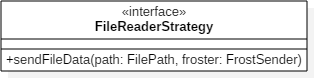
\includegraphics[width=0.5\linewidth]{images/import/classes/FileReaderStrategy}
\end{figure}
\subsubsection{Declaration}{
\begin{lstlisting}[frame=none]
public interface FileReaderStrategy
\end{lstlisting}
\subsubsection{All known subinterfaces}{NetCDFReaderStrategy\small{\refdefined{Import.NetCDFReaderStrategy}}, CSVReaderStrategy\small{\refdefined{Import.CSVReaderStrategy}}}
\subsubsection{All classes known to implement interface}{NetCDFReaderStrategy\small{\refdefined{Import.NetCDFReaderStrategy}}, CSVReaderStrategy\small{\refdefined{Import.CSVReaderStrategy}}}
\subsubsection{Method summary}{
\begin{verse}
\hyperlink{Import.FileReaderStrategy.sendFileData(FilePath, Import.FrostSender)}{{\bf sendFileData(FilePath, FrostSender)}} Reades from a File as specified by the FilePath and sends the information in it to the FROST-Server using the FrostSender that was provided.\\
\end{verse}
}
\subsubsection{Methods}{
\vskip -2em
\begin{itemize}
\item{
\index{sendFileData(FilePath, FrostSender)}
\hypertarget{Import.FileReaderStrategy.sendFileData(FilePath, Import.FrostSender)}{{\bf  sendFileData}\\}
\begin{lstlisting}[frame=none]
void sendFileData(FilePath path,FrostSender froster)\end{lstlisting} %end signature
\begin{itemize}
\item{
{\bf  Description}

Reades from a File as specified by the FilePath and sends the information in it to the FROST-Server using the FrostSender that was provided.
}
\item{
{\bf  Parameters}
  \begin{itemize}
   \item{
\texttt{path} -- Is the FilePath of the File to Import.}
   \item{
\texttt{froster} -- Is the FrostSender instance that will be used to send the files data to the Frost-Server.}
  \end{itemize}
}%end item
\end{itemize}
}%end item
\end{itemize}
}
}
\subsection{\label{Import.CSVReaderStrategy}Class CSVReaderStrategy}{
\hypertarget{Import.CSVReaderStrategy}{}\vskip .1in
Implementation of the FileReaderStrategy interface for CSV files.\vskip .1in
\begin{figure}[!hbp]
	\centering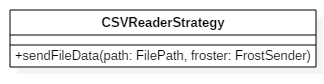
\includegraphics[width=0.5\linewidth]{images/import/classes/CSVReaderStrategy}
\end{figure}
\subsubsection{Declaration}{
\begin{lstlisting}[frame=none]
public class CSVReaderStrategy
 extends java.lang.Object implements FileReaderStrategy\end{lstlisting}
\subsubsection{Constructor summary}{
\begin{verse}
\hyperlink{Import.CSVReaderStrategy()}{{\bf CSVReaderStrategy()}} Default constructor\\
\end{verse}
}
\subsubsection{Method summary}{
\begin{verse}
\hyperlink{Import.CSVReaderStrategy.sendFileData(FilePath, Import.FrostSender)}{{\bf sendFileData(FilePath, FrostSender)}} Reades from a File as specified by the FilePath and sends the information in it to the FROST-Server using the FrostSender that was provided.\\
\hyperlink{Import.CSVReaderStrategy.sendFileData(FilePath, Import.FrostSender)}{{\bf sendFileData(FilePath, FrostSender)}} Reades from a File as specified by the FilePath and sends the information in it to the FROST-Server using the FrostSender that was provided.\\
\end{verse}
}
\subsubsection{Constructors}{
\vskip -2em
\begin{itemize}
\item{
\index{CSVReaderStrategy()}
\hypertarget{Import.CSVReaderStrategy()}{{\bf  CSVReaderStrategy}\\}
\begin{lstlisting}[frame=none]
public CSVReaderStrategy()\end{lstlisting} %end signature
\begin{itemize}
\item{
{\bf  Description}

Default constructor
}
\end{itemize}
}%end item
\end{itemize}
}
\subsubsection{Methods}{
\vskip -2em
\begin{itemize}
\item{
\index{sendFileData(FilePath, FrostSender)}
\hypertarget{Import.CSVReaderStrategy.sendFileData(FilePath, Import.FrostSender)}{{\bf  sendFileData}\\}
\begin{lstlisting}[frame=none]
public void sendFileData(FilePath path,FrostSender froster)\end{lstlisting} %end signature
\begin{itemize}
\item{
{\bf  Description}

Reades from a File as specified by the FilePath and sends the information in it to the FROST-Server using the FrostSender that was provided.
}
\item{
{\bf  Parameters}
  \begin{itemize}
   \item{
\texttt{path} -- Is the FilePath of the File to Import.}
   \item{
\texttt{froster} -- Is the FrostSender instance that will be used to send the files data to the Frost-Server.}
  \end{itemize}
}%end item
\end{itemize}
}%end item
\item{
\index{sendFileData(FilePath, FrostSender)}
\hypertarget{Import.CSVReaderStrategy.sendFileData(FilePath, Import.FrostSender)}{{\bf  sendFileData}\\}
\begin{lstlisting}[frame=none]
public void sendFileData(FilePath path,FrostSender froster)\end{lstlisting} %end signature
\begin{itemize}
\item{
{\bf  Description}

Reades from a File as specified by the FilePath and sends the information in it to the FROST-Server using the FrostSender that was provided.
}
\item{
{\bf  Parameters}
  \begin{itemize}
   \item{
\texttt{path} -- Is the FilePath of the File to Import.}
   \item{
\texttt{froster} -- Is the FrostSender instance that will be used to send the files data to the Frost-Server.}
  \end{itemize}
}%end item
\end{itemize}
}%end item
\end{itemize}
}
}
\subsection{\label{Import.DataImporter}Class DataImporter}{
\hypertarget{Import.DataImporter}{}\vskip .1in
Importer for data that should be added to PaVoS. Import takes place for files in a specified folder of the server.\vskip .1in
\begin{figure}[!hbp]
	\centering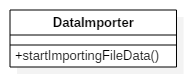
\includegraphics[width=0.5\linewidth]{images/import/classes/DataImporter}
\end{figure}
\subsubsection{Declaration}{
\begin{lstlisting}[frame=none]
public class DataImporter
 extends java.lang.Object\end{lstlisting}
\subsubsection{Constructor summary}{
\begin{verse}
\hyperlink{Import.DataImporter()}{{\bf DataImporter()}} Default constructor\\
\end{verse}
}
\subsubsection{Method summary}{
\begin{verse}
\hyperlink{Import.DataImporter.startImportingFileData()}{{\bf startImportingFileData()}} Checks for files in the specified import folder and opens a new thread for each of them, where a FileImporter is started to import the contained data.\\
\end{verse}
}
\subsubsection{Constructors}{
\vskip -2em
\begin{itemize}
\item{
\index{DataImporter()}
\hypertarget{Import.DataImporter()}{{\bf  DataImporter}\\}
\begin{lstlisting}[frame=none]
public DataImporter()\end{lstlisting} %end signature
\begin{itemize}
\item{
{\bf  Description}

Default constructor
}
\end{itemize}
}%end item
\end{itemize}
}
\subsubsection{Methods}{
\vskip -2em
\begin{itemize}
\item{
\index{startImportingFileData()}
\hypertarget{Import.DataImporter.startImportingFileData()}{{\bf  startImportingFileData}\\}
\begin{lstlisting}[frame=none]
public void startImportingFileData()\end{lstlisting} %end signature
\begin{itemize}
\item{
{\bf  Description}

Checks for files in the specified import folder and opens a new thread for each of them, where a FileImporter is started to import the contained data.
}
\end{itemize}
}%end item
\end{itemize}
}
}
\subsection{\label{Import.FileImporter}Class FileImporter}{
\hypertarget{Import.FileImporter}{}\vskip .1in
Importer for the Data contained in a File. Takes the Data and sends them to the FROST-Server.\vskip .1in
\begin{figure}[!hbp]
	\centering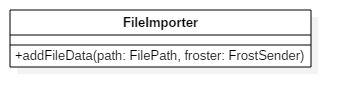
\includegraphics[width=0.5\linewidth]{images/import/classes/FileImporter}
\end{figure}
\subsubsection{Declaration}{
\begin{lstlisting}[frame=none]
public class FileImporter
 extends java.lang.Object\end{lstlisting}
\subsubsection{Constructor summary}{
\begin{verse}
\hyperlink{Import.FileImporter()}{{\bf FileImporter()}} Default constructor\\
\end{verse}
}
\subsubsection{Method summary}{
\begin{verse}
\hyperlink{Import.FileImporter.addFileData(FilePath, Import.FrostSender)}{{\bf addFileData(FilePath, FrostSender)}} Adds the Data of a File at a specified FilePath to the FROST-Server.\\
\end{verse}
}
\subsubsection{Constructors}{
\vskip -2em
\begin{itemize}
\item{
\index{FileImporter()}
\hypertarget{Import.FileImporter()}{{\bf  FileImporter}\\}
\begin{lstlisting}[frame=none]
public FileImporter()\end{lstlisting} %end signature
\begin{itemize}
\item{
{\bf  Description}

Default constructor
}
\end{itemize}
}%end item
\end{itemize}
}
\subsubsection{Methods}{
\vskip -2em
\begin{itemize}
\item{
\index{addFileData(FilePath, FrostSender)}
\hypertarget{Import.FileImporter.addFileData(FilePath, Import.FrostSender)}{{\bf  addFileData}\\}
\begin{lstlisting}[frame=none]
public void addFileData(FilePath path,FrostSender froster)\end{lstlisting} %end signature
\begin{itemize}
\item{
{\bf  Description}

Adds the Data of a File at a specified FilePath to the FROST-Server. To do so, the FileExtension of the File is determined.With help of the readerTypeClass the matching implementation of the FileReaderStrategy interface for the FileExtension is generated and can be used to get the Data from then File.
}
\item{
{\bf  Parameters}
  \begin{itemize}
   \item{
\texttt{path} -- Is the FilePath of the File to Import.}
   \item{
\texttt{froster} -- Is the FrostSender instance that will be used to send the files data to the Frost-Server.}
  \end{itemize}
}%end item
\end{itemize}
}%end item
\end{itemize}
}
}
\subsection{\label{Import.FrostSender}Class FrostSender}{
\hypertarget{Import.FrostSender}{}\vskip .1in
sends Data to the FROST-Server.\vskip .1in
\begin{figure}[!hbp]
	\centering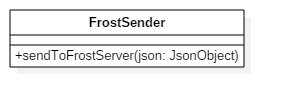
\includegraphics[width=0.5\linewidth]{images/import/classes/FrostSender}
\end{figure}
\subsubsection{Declaration}{
\begin{lstlisting}[frame=none]
public class FrostSender
 extends java.lang.Object\end{lstlisting}
\subsubsection{Constructor summary}{
\begin{verse}
\hyperlink{Import.FrostSender()}{{\bf FrostSender()}} Default constructor\\
\end{verse}
}
\subsubsection{Method summary}{
\begin{verse}
\hyperlink{Import.FrostSender.sendToFrostServer(JsonObject)}{{\bf sendToFrostServer(JsonObject)}} Sends the given JsonObject to the FROST-Server.\\
\end{verse}
}
\subsubsection{Constructors}{
\vskip -2em
\begin{itemize}
\item{
\index{FrostSender()}
\hypertarget{Import.FrostSender()}{{\bf  FrostSender}\\}
\begin{lstlisting}[frame=none]
public FrostSender()\end{lstlisting} %end signature
\begin{itemize}
\item{
{\bf  Description}

Default constructor
}
\end{itemize}
}%end item
\end{itemize}
}
\subsubsection{Methods}{
\vskip -2em
\begin{itemize}
\item{
\index{sendToFrostServer(JsonObject)}
\hypertarget{Import.FrostSender.sendToFrostServer(JsonObject)}{{\bf  sendToFrostServer}\\}
\begin{lstlisting}[frame=none]
public void sendToFrostServer(JsonObject json)\end{lstlisting} %end signature
\begin{itemize}
\item{
{\bf  Description}

Sends the given JsonObject to the FROST-Server.
}
\item{
{\bf  Parameters}
  \begin{itemize}
   \item{
\texttt{json} -- Represents a single ObservedProperty.}
  \end{itemize}
}%end item
\end{itemize}
}%end item
\end{itemize}
}
}
\subsection{\label{Import.NetCDFReaderStrategy}Class NetCDFReaderStrategy}{
\hypertarget{Import.NetCDFReaderStrategy}{}\vskip .1in
Implementation of the FileReaderStrategy interface for NetCDF files.\vskip .1in
\begin{figure}[!hbp]
	\centering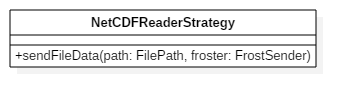
\includegraphics[width=0.5\linewidth]{images/import/classes/NetCDFReaderStrategy}
\end{figure}
\subsubsection{Declaration}{
\begin{lstlisting}[frame=none]
public class NetCDFReaderStrategy
 extends java.lang.Object implements FileReaderStrategy\end{lstlisting}
\subsubsection{Constructor summary}{
\begin{verse}
\hyperlink{Import.NetCDFReaderStrategy()}{{\bf NetCDFReaderStrategy()}} Default constructor\\
\end{verse}
}
\subsubsection{Method summary}{
\begin{verse}
\hyperlink{Import.NetCDFReaderStrategy.sendFileData(FilePath, Import.FrostSender)}{{\bf sendFileData(FilePath, FrostSender)}} Reades from a File as specified by the FilePath and sends the information in it to the FROST-Server using the FrostSender that was provided.\\
\hyperlink{Import.NetCDFReaderStrategy.sendFileData(FilePath, Import.FrostSender)}{{\bf sendFileData(FilePath, FrostSender)}} Reades from a File as specified by the FilePath and sends the information in it to the FROST-Server using the FrostSender that was provided.\\
\end{verse}
}
\subsubsection{Constructors}{
\vskip -2em
\begin{itemize}
\item{
\index{NetCDFReaderStrategy()}
\hypertarget{Import.NetCDFReaderStrategy()}{{\bf  NetCDFReaderStrategy}\\}
\begin{lstlisting}[frame=none]
public NetCDFReaderStrategy()\end{lstlisting} %end signature
\begin{itemize}
\item{
{\bf  Description}

Default constructor
}
\end{itemize}
}%end item
\end{itemize}
}
\subsubsection{Methods}{
\vskip -2em
\begin{itemize}
\item{
\index{sendFileData(FilePath, FrostSender)}
\hypertarget{Import.NetCDFReaderStrategy.sendFileData(FilePath, Import.FrostSender)}{{\bf  sendFileData}\\}
\begin{lstlisting}[frame=none]
public void sendFileData(FilePath path,FrostSender froster)\end{lstlisting} %end signature
\begin{itemize}
\item{
{\bf  Description}

Reades from a File as specified by the FilePath and sends the information in it to the FROST-Server using the FrostSender that was provided.
}
\item{
{\bf  Parameters}
  \begin{itemize}
   \item{
\texttt{path} -- Is the FilePath of the File to Import.}
   \item{
\texttt{froster} -- Is the FrostSender instance that will be used to send the files data to the Frost-Server.}
  \end{itemize}
}%end item
\end{itemize}
}%end item
\item{
\index{sendFileData(FilePath, FrostSender)}
\hypertarget{Import.NetCDFReaderStrategy.sendFileData(FilePath, Import.FrostSender)}{{\bf  sendFileData}\\}
\begin{lstlisting}[frame=none]
public void sendFileData(FilePath path,FrostSender froster)\end{lstlisting} %end signature
\begin{itemize}
\item{
{\bf  Description}

Reades from a File as specified by the FilePath and sends the information in it to the FROST-Server using the FrostSender that was provided.
}
\item{
{\bf  Parameters}
  \begin{itemize}
   \item{
\texttt{path} -- Is the FilePath of the File to Import.}
   \item{
\texttt{froster} -- Is the FrostSender instance that will be used to send the files data to the Frost-Server.}
  \end{itemize}
}%end item
\end{itemize}
}%end item
\end{itemize}
}
}
\subsection{\label{Import.ReaderType}Class ReaderType}{
\hypertarget{Import.ReaderType}{}\vskip .1in
Is like a chooser for the right FileReaderStrategy. If a new Strategy is added, this class needs some changes to use the new Strategy.\vskip .1in 
\begin{figure}[!hbp]
	\centering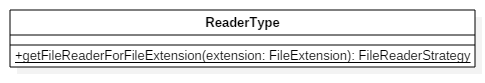
\includegraphics[width=0.5\linewidth]{images/import/classes/ReaderType}
\end{figure}
\subsubsection{Declaration}{
\begin{lstlisting}[frame=none]
public class ReaderType
 extends java.lang.Object\end{lstlisting}
\subsubsection{Constructor summary}{
\begin{verse}
\hyperlink{Import.ReaderType()}{{\bf ReaderType()}} Default constructor\\
\end{verse}
}
\subsubsection{Method summary}{
\begin{verse}
\hyperlink{Import.ReaderType.getFileReaderForFileExtension(FileExtension)}{{\bf getFileReaderForFileExtension(FileExtension)}} Gives a new Instance of a FileReaderStrategy for the specified FileExtension.\\
\end{verse}
}
\subsubsection{Constructors}{
\vskip -2em
\begin{itemize}
\item{
\index{ReaderType()}
\hypertarget{Import.ReaderType()}{{\bf  ReaderType}\\}
\begin{lstlisting}[frame=none]
public ReaderType()\end{lstlisting} %end signature
\begin{itemize}
\item{
{\bf  Description}

Default constructor
}
\end{itemize}
}%end item
\end{itemize}
}
\subsubsection{Methods}{
\vskip -2em
\begin{itemize}
\item{
\index{getFileReaderForFileExtension(FileExtension)}
\hypertarget{Import.ReaderType.getFileReaderForFileExtension(FileExtension)}{{\bf  getFileReaderForFileExtension}\\}
\begin{lstlisting}[frame=none]
public static FileReaderStrategy getFileReaderForFileExtension(FileExtension extension)\end{lstlisting} %end signature
\begin{itemize}
\item{
{\bf  Description}

Gives a new Instance of a FileReaderStrategy for the specified FileExtension.
}
\item{
{\bf  Parameters}
  \begin{itemize}
   \item{
\texttt{extension} -- is the FileExtension for which a FileReaderStrategy has to be generated.}
  \end{itemize}
}%end item
\item{{\bf  Returns} --
An instance of an implementation of the FileReaderStrategy interface.
}%end item
\end{itemize}
}%end item
\end{itemize}
}
}
}

	\chapter{Database}
\section{Package DatabaseConnection}{
\label{DatabaseConnection}\hypertarget{DatabaseConnection}{}
\hskip -.05in
\hbox to \hsize{\textit{ Package Contents\hfil Page}}
\vskip .13in
\hbox{{\bf  Classes}}
\entityintro{ClusterID}{DatabaseConnection.ClusterID}{This class describes a unique identification of a cluster via longitude and latitude.}
\entityintro{DataMaintainer}{DatabaseConnection.DataMaintainer}{This class maintains the sensordata in the StorageSolution.}
\entityintro{Facade}{DatabaseConnection.Facade}{A facade to simplify access to a StorageSolution, such as a database.}
\entityintro{GridDataServlet}{DatabaseConnection.GridDataServlet}{An HTTPServlet for requesting Grid data.}
\entityintro{HttpServlet}{DatabaseConnection.HttpServlet}{An abstract HTTPServlet.}
\entityintro{KafkaToStorageProcessor}{DatabaseConnection.KafkaToStorageProcessor}{This class converts KafkaStream records to data that can be inserted into the StorageSolution.}
\entityintro{Maintainer}{DatabaseConnection.Maintainer}{An abstract class describing a Maintainer, which performs maintenance on certain data in the StorageSolution.}
\entityintro{MaintenanceManager}{DatabaseConnection.MaintenanceManager}{This class manages the way the methods of Maintainers are called to make sure the StorageSolution content is maintained.}
\entityintro{SensorListServlet}{DatabaseConnection.SensorListServlet}{An HTTPServlet for requesting a list of sensors.}
\entityintro{SensorMaintainer}{DatabaseConnection.SensorMaintainer}{This class maintains the list of sensors saved in the StorageSolution.}
\entityintro{ZoomLevel}{DatabaseConnection.ZoomLevel}{This class describes a zoom level for the map.}
\vskip .1in
\vskip .1in
\subsection{\label{DatabaseConnection.ClusterID}Class ClusterID}{
\hypertarget{DatabaseConnection.ClusterID}{}\vskip .1in
This class describes a unique identification of a cluster via longitude and latitude.\vskip .1in
\begin{figure}[!hbp]
	\centering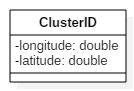
\includegraphics[width=0.2\linewidth]{images/database/classes/ClusterID}
\end{figure}
\subsubsection{Declaration}{
\begin{lstlisting}[frame=none]
public class ClusterID
 extends java.lang.Object\end{lstlisting}
\subsubsection{Constructor summary}{
\begin{verse}
\hyperlink{DatabaseConnection.ClusterID()}{{\bf ClusterID()}} Default constructor\\
\end{verse}
}
\subsubsection{Constructors}{
\vskip -2em
\begin{itemize}
\item{
\index{ClusterID()}
\hypertarget{DatabaseConnection.ClusterID()}{{\bf  ClusterID}\\}
\begin{lstlisting}[frame=none]
public ClusterID()\end{lstlisting} %end signature
\begin{itemize}
\item{
{\bf  Description}

Default constructor
}
\end{itemize}
}%end item
\end{itemize}
}
}
\subsection{\label{DatabaseConnection.DataMaintainer}Class DataMaintainer}{
\hypertarget{DatabaseConnection.DataMaintainer}{}\vskip .1in
This class maintains the sensordata in the StorageSolution.\vskip .1in
\begin{figure}[!hbp]
	\centering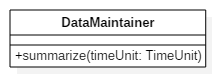
\includegraphics[width=0.4\linewidth]{images/database/classes/DataMaintainer}
\end{figure}
\subsubsection{Declaration}{
\begin{lstlisting}[frame=none]
public class DataMaintainer
 extends DatabaseConnection.Maintainer\end{lstlisting}
\subsubsection{Constructor summary}{
\begin{verse}
\hyperlink{DatabaseConnection.DataMaintainer()}{{\bf DataMaintainer()}} Default constructor\\
\end{verse}
}
\subsubsection{Method summary}{
\begin{verse}
\hyperlink{DatabaseConnection.DataMaintainer.summarize(TimeUnit)}{{\bf summarize(TimeUnit)}} This method takes data of a certain TimeUnit and summarizes it into the next higher TimeUnit.\\
\end{verse}
}
\subsubsection{Constructors}{
\vskip -2em
\begin{itemize}
\item{
\index{DataMaintainer()}
\hypertarget{DatabaseConnection.DataMaintainer()}{{\bf  DataMaintainer}\\}
\begin{lstlisting}[frame=none]
public DataMaintainer()\end{lstlisting} %end signature
\begin{itemize}
\item{
{\bf  Description}

Default constructor
}
\end{itemize}
}%end item
\end{itemize}
}
\subsubsection{Methods}{
\vskip -2em
\begin{itemize}
\item{
\index{summarize(TimeUnit)}
\hypertarget{DatabaseConnection.DataMaintainer.summarize(TimeUnit)}{{\bf  summarize}\\}
\begin{lstlisting}[frame=none]
public void summarize(TimeUnit timeUnit)\end{lstlisting} %end signature
\begin{itemize}
\item{
{\bf  Description}

This method takes data of a certain TimeUnit and summarizes it into the next higher TimeUnit. The summarized data is then saved back into the StorageSolution. The original data of the lower TimeUnit is then deleted from the database.
}
\item{
{\bf  Parameters}
  \begin{itemize}
   \item{
\texttt{timeUnit} -- The TimeUnit to summarize.}
  \end{itemize}
}%end item
\end{itemize}
}%end item
\end{itemize}
}
}
\subsection{\label{DatabaseConnection.Facade}Class Facade}{
\hypertarget{DatabaseConnection.Facade}{}\vskip .1in
A facade to simplify access to a StorageSolution, such as a database. Through the methods, data can be inserted into the StorageSolution and certain information about its content requested.\vskip .1in
\begin{figure}[!hbp]
	\centering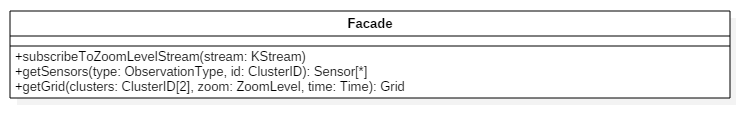
\includegraphics[width=0.9\linewidth]{images/database/classes/Facade}
\end{figure}
\subsubsection{Declaration}{
\begin{lstlisting}[frame=none]
public class Facade
 extends java.lang.Object\end{lstlisting}
\subsubsection{Constructor summary}{
\begin{verse}
\hyperlink{DatabaseConnection.Facade()}{{\bf Facade()}} Default constructor\\
\end{verse}
}
\subsubsection{Method summary}{
\begin{verse}
\hyperlink{DatabaseConnection.Facade.getGrid(DatabaseConnection.ClusterID[], DatabaseConnection.ZoomLevel, Time)}{{\bf getGrid(ClusterID\lbrack \rbrack , ZoomLevel, Time)}} Returns an appropriate grid of clusters in the requested grid section for the specified ZoomLevel and time.\\
\hyperlink{DatabaseConnection.Facade.getSensors(ObservationType, DatabaseConnection.ClusterID)}{{\bf getSensors(ObservationType, ClusterID)}} Fetches all sensors from the given cluster that observe the given ObservedProperty and returns an array of sensors.\\
\hyperlink{DatabaseConnection.Facade.subscribeToZoomLevelStream(KStream)}{{\bf subscribeToZoomLevelStream(KStream)}} Subscribes to the given KafkaStream, which contains ZoomLevel-specific data and initiates processing of its records.\\
\end{verse}
}
\subsubsection{Constructors}{
\vskip -2em
\begin{itemize}
\item{
\index{Facade()}
\hypertarget{DatabaseConnection.Facade()}{{\bf  Facade}\\}
\begin{lstlisting}[frame=none]
public Facade()\end{lstlisting} %end signature
\begin{itemize}
\item{
{\bf  Description}

Default constructor
}
\end{itemize}
}%end item
\end{itemize}
}
\subsubsection{Methods}{
\vskip -2em
\begin{itemize}
\item{
\index{getGrid(ClusterID\lbrack \rbrack , ZoomLevel, Time)}
\hypertarget{DatabaseConnection.Facade.getGrid(DatabaseConnection.ClusterID[], DatabaseConnection.ZoomLevel, Time)}{{\bf  getGrid}\\}
\begin{lstlisting}[frame=none]
public Grid getGrid(ClusterID[] clusters,ZoomLevel zoom,Time time)\end{lstlisting} %end signature
\begin{itemize}
\item{
{\bf  Description}

Returns an appropriate grid of clusters in the requested grid section for the specified ZoomLevel and time. The (first) two values of the ClusterID array define the grid section from which to get the data.
}
\item{
{\bf  Parameters}
  \begin{itemize}
   \item{
\texttt{clusters} -- An array of ClusterIDs from which the first two entries are taken to compute the section of the Grid to get the data from.}
   \item{
\texttt{zoom} -- The ZoomLevel from which to get the data.}
   \item{
\texttt{time} -- The point in time.}
  \end{itemize}
}%end item
\item{{\bf  Returns} --
A grid with the computed data.
}%end item
\end{itemize}
}%end item
\item{
\index{getSensors(ObservationType, ClusterID)}
\hypertarget{DatabaseConnection.Facade.getSensors(ObservationType, DatabaseConnection.ClusterID)}{{\bf  getSensors}\\}
\begin{lstlisting}[frame=none]
public java.util.Set getSensors(ObservationType type,ClusterID id)\end{lstlisting} %end signature
\begin{itemize}
\item{
{\bf  Description}

Fetches all sensors from the given cluster that observe the given ObservedProperty and returns an array of sensors.
}
\item{
{\bf  Parameters}
  \begin{itemize}
   \item{
\texttt{type} -- The ObservationType of the requested sensors.}
   \item{
\texttt{id} -- The ID of the cluster.}
  \end{itemize}
}%end item
\item{{\bf  Returns} --
An array of sensors.
}%end item
\end{itemize}
}%end item
\item{
\index{subscribeToZoomLevelStream(KStream)}
\hypertarget{DatabaseConnection.Facade.subscribeToZoomLevelStream(KStream)}{{\bf  subscribeToZoomLevelStream}\\}
\begin{lstlisting}[frame=none]
public void subscribeToZoomLevelStream(KStream stream)\end{lstlisting} %end signature
\begin{itemize}
\item{
{\bf  Description}

Subscribes to the given KafkaStream, which contains ZoomLevel-specific data and initiates processing of its records.
}
\item{
{\bf  Parameters}
  \begin{itemize}
   \item{
\texttt{stream} -- The stream to subscribe to.}
  \end{itemize}
}%end item
\end{itemize}
}%end item
\end{itemize}
}
}
\subsection{\label{DatabaseConnection.GridDataServlet}Class GridDataServlet}{
\hypertarget{DatabaseConnection.GridDataServlet}{}\vskip .1in
An HTTPServlet for requesting Grid data.\vskip .1in
\begin{figure}[!hbp]
	\centering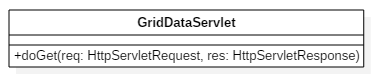
\includegraphics[width=0.6\linewidth]{images/database/classes/GridDataServlet}
\end{figure}
\subsubsection{Declaration}{
\begin{lstlisting}[frame=none]
public class GridDataServlet
 extends DatabaseConnection.HttpServlet\end{lstlisting}
\subsubsection{Constructor summary}{
\begin{verse}
\hyperlink{DatabaseConnection.GridDataServlet()}{{\bf GridDataServlet()}} Default constructor\\
\end{verse}
}
\subsubsection{Method summary}{
\begin{verse}
\hyperlink{DatabaseConnection.GridDataServlet.doGet(HttpServletRequest, HttpServletResponse)}{{\bf doGet(HttpServletRequest, HttpServletResponse)}} This method calls the getGrid method of the Facade to get a Grid of clusters at a certain ZoomLevel and Time .\\
\end{verse}
}
\subsubsection{Constructors}{
\vskip -2em
\begin{itemize}
\item{
\index{GridDataServlet()}
\hypertarget{DatabaseConnection.GridDataServlet()}{{\bf  GridDataServlet}\\}
\begin{lstlisting}[frame=none]
public GridDataServlet()\end{lstlisting} %end signature
\begin{itemize}
\item{
{\bf  Description}

Default constructor
}
\end{itemize}
}%end item
\end{itemize}
}
\subsubsection{Methods}{
\vskip -2em
\begin{itemize}
\item{
\index{doGet(HttpServletRequest, HttpServletResponse)}
\hypertarget{DatabaseConnection.GridDataServlet.doGet(HttpServletRequest, HttpServletResponse)}{{\bf  doGet}\\}
\begin{lstlisting}[frame=none]
public void doGet(HttpServletRequest req,HttpServletResponse res)\end{lstlisting} %end signature
\begin{itemize}
\item{
{\bf  Description}

This method calls the getGrid method of the Facade to get a Grid of clusters at a certain ZoomLevel and Time . This saves the Grid into res.
}
\item{
{\bf  Parameters}
  \begin{itemize}
   \item{
\texttt{req} -- An HttpServletRequest object that contains the request the client has made of the servlet.}
   \item{
\texttt{res} -- An HttpServletResponse object that contains the response the servlet sends to the client.}
  \end{itemize}
}%end item
\end{itemize}
}%end item
\end{itemize}
}
\subsubsection{Members inherited from class HttpServlet }{
\texttt{DatabaseConnection.HttpServlet} {\small
\refdefined{DatabaseConnection.HttpServlet}}
{\small

\vskip -2em
\begin{itemize}
\item{\vskip -1.5ex
\texttt{public void {\bf  doGet}(\texttt{HttpServletRequest} {\bf  req},
\texttt{HttpServletResponse} {\bf  res})
}%end signature
}%end item
\end{itemize}
}
}
\subsection{\label{DatabaseConnection.HttpServlet}Class HttpServlet}{
\hypertarget{DatabaseConnection.HttpServlet}{}\vskip .1in
An abstract HTTPServlet.\vskip .1in
\begin{figure}[!hbp]
	\centering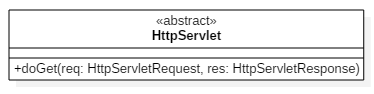
\includegraphics[width=0.6\linewidth]{images/database/classes/HttpServlet}
\end{figure}
\subsubsection{Declaration}{
\begin{lstlisting}[frame=none]
public class HttpServlet
 extends java.lang.Object\end{lstlisting}
\subsubsection{All known subclasses}{SensorListServlet\small{\refdefined{DatabaseConnection.SensorListServlet}}, GridDataServlet\small{\refdefined{DatabaseConnection.GridDataServlet}}}
\subsubsection{Constructor summary}{
\begin{verse}
\hyperlink{DatabaseConnection.HttpServlet()}{{\bf HttpServlet()}} Default constructor\\
\end{verse}
}
\subsubsection{Method summary}{
\begin{verse}
\hyperlink{DatabaseConnection.HttpServlet.doGet(HttpServletRequest, HttpServletResponse)}{{\bf doGet(HttpServletRequest, HttpServletResponse)}} Called by the server (via the service method) to allow a servlet to handle a GET request.\\
\end{verse}
}
\subsubsection{Constructors}{
\vskip -2em
\begin{itemize}
\item{
\index{HttpServlet()}
\hypertarget{DatabaseConnection.HttpServlet()}{{\bf  HttpServlet}\\}
\begin{lstlisting}[frame=none]
public HttpServlet()\end{lstlisting} %end signature
\begin{itemize}
\item{
{\bf  Description}

Default constructor
}
\end{itemize}
}%end item
\end{itemize}
}
\subsubsection{Methods}{
\vskip -2em
\begin{itemize}
\item{
\index{doGet(HttpServletRequest, HttpServletResponse)}
\hypertarget{DatabaseConnection.HttpServlet.doGet(HttpServletRequest, HttpServletResponse)}{{\bf  doGet}\\}
\begin{lstlisting}[frame=none]
public void doGet(HttpServletRequest req,HttpServletResponse res)\end{lstlisting} %end signature
\begin{itemize}
\item{
{\bf  Description}

Called by the server (via the service method) to allow a servlet to handle a GET request.
}
\item{
{\bf  Parameters}
  \begin{itemize}
   \item{
\texttt{req} -- An HttpServletRequest object that contains the request the client has made of the servlet.}
   \item{
\texttt{res} -- An HttpServletResponse object that contains the response the servlet sends to the client.}
  \end{itemize}
}%end item
\end{itemize}
}%end item
\end{itemize}
}
}
\subsection{\label{DatabaseConnection.KafkaToStorageProcessor}Class KafkaToStorageProcessor}{
\hypertarget{DatabaseConnection.KafkaToStorageProcessor}{}\vskip .1in
This class converts KafkaStream records to data that can be inserted into the StorageSolution.\vskip .1in
\begin{figure}[!hbp]
	\centering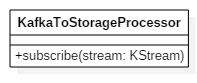
\includegraphics[width=0.5\linewidth]{images/database/classes/KafkaToStorageProcessor}
\end{figure}
\subsubsection{Declaration}{
\begin{lstlisting}[frame=none]
public class KafkaToStorageProcessor
 extends java.lang.Object\end{lstlisting}
\subsubsection{Constructor summary}{
\begin{verse}
\hyperlink{DatabaseConnection.KafkaToStorageProcessor()}{{\bf KafkaToStorageProcessor()}} Default constructor\\
\end{verse}
}
\subsubsection{Method summary}{
\begin{verse}
\hyperlink{DatabaseConnection.KafkaToStorageProcessor.subscribe(KStream)}{{\bf subscribe(KStream)}} Subscribes to the given KafkaStream and converts the data to the appropriate format for the StorageSolution.\\
\end{verse}
}
\subsubsection{Constructors}{
\vskip -2em
\begin{itemize}
\item{
\index{KafkaToStorageProcessor()}
\hypertarget{DatabaseConnection.KafkaToStorageProcessor()}{{\bf  KafkaToStorageProcessor}\\}
\begin{lstlisting}[frame=none]
public KafkaToStorageProcessor()\end{lstlisting} %end signature
\begin{itemize}
\item{
{\bf  Description}

Default constructor
}
\end{itemize}
}%end item
\end{itemize}
}
\subsubsection{Methods}{
\vskip -2em
\begin{itemize}
\item{
\index{subscribe(KStream)}
\hypertarget{DatabaseConnection.KafkaToStorageProcessor.subscribe(KStream)}{{\bf  subscribe}\\}
\begin{lstlisting}[frame=none]
public void subscribe(KStream stream)\end{lstlisting} %end signature
\begin{itemize}
\item{
{\bf  Description}

Subscribes to the given KafkaStream and converts the data to the appropriate format for the StorageSolution. If a stream is already subscribed to, unsubscribes from the old stream and subscribes to the new one.
}
\item{
{\bf  Parameters}
  \begin{itemize}
   \item{
\texttt{stream} -- The KStream to subscribe to.}
  \end{itemize}
}%end item
\end{itemize}
}%end item
\end{itemize}
}
}
\subsection{\label{DatabaseConnection.Maintainer}Class Maintainer}{
\hypertarget{DatabaseConnection.Maintainer}{}\vskip .1in
An abstract class describing a Maintainer, which performs maintenance on certain data in the StorageSolution.\vskip .1in
\begin{figure}[!hbp]
	\centering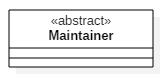
\includegraphics[width=0.4\linewidth]{images/database/classes/Maintainer}
\end{figure}
\subsubsection{Declaration}{
\begin{lstlisting}[frame=none]
public class Maintainer
 extends java.lang.Object\end{lstlisting}
\subsubsection{All known subclasses}{SensorMaintainer\small{\refdefined{DatabaseConnection.SensorMaintainer}}, DataMaintainer\small{\refdefined{DatabaseConnection.DataMaintainer}}}
\subsubsection{Constructor summary}{
\begin{verse}
\hyperlink{DatabaseConnection.Maintainer()}{{\bf Maintainer()}} Default constructor\\
\end{verse}
}
\subsubsection{Constructors}{
\vskip -2em
\begin{itemize}
\item{
\index{Maintainer()}
\hypertarget{DatabaseConnection.Maintainer()}{{\bf  Maintainer}\\}
\begin{lstlisting}[frame=none]
public Maintainer()\end{lstlisting} %end signature
\begin{itemize}
\item{
{\bf  Description}

Default constructor
}
\end{itemize}
}%end item
\end{itemize}
}
}
\subsection{\label{DatabaseConnection.MaintenanceManager}Class MaintenanceManager}{
\hypertarget{DatabaseConnection.MaintenanceManager}{}\vskip .1in
This class manages the way the methods of Maintainers are called to make sure the StorageSolution content is maintained.\vskip .1in
\begin{figure}[!hbp]
	\centering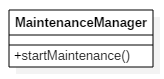
\includegraphics[width=0.4\linewidth]{images/database/classes/MaintenanceManager}
\end{figure}
\subsubsection{Declaration}{
\begin{lstlisting}[frame=none]
public class MaintenanceManager
 extends java.lang.Object\end{lstlisting}
\subsubsection{Constructor summary}{
\begin{verse}
\hyperlink{DatabaseConnection.MaintenanceManager()}{{\bf MaintenanceManager()}} Default constructor\\
\end{verse}
}
\subsubsection{Method summary}{
\begin{verse}
\hyperlink{DatabaseConnection.MaintenanceManager.startMaintenance()}{{\bf startMaintenance()}} This method should be called as soon as the database is started.\\
\end{verse}
}
\subsubsection{Constructors}{
\vskip -2em
\begin{itemize}
\item{
\index{MaintenanceManager()}
\hypertarget{DatabaseConnection.MaintenanceManager()}{{\bf  MaintenanceManager}\\}
\begin{lstlisting}[frame=none]
public MaintenanceManager()\end{lstlisting} %end signature
\begin{itemize}
\item{
{\bf  Description}

Default constructor
}
\end{itemize}
}%end item
\end{itemize}
}
\subsubsection{Methods}{
\vskip -2em
\begin{itemize}
\item{
\index{startMaintenance()}
\hypertarget{DatabaseConnection.MaintenanceManager.startMaintenance()}{{\bf  startMaintenance}\\}
\begin{lstlisting}[frame=none]
public void startMaintenance()\end{lstlisting} %end signature
\begin{itemize}
\item{
{\bf  Description}

This method should be called as soon as the database is started. Through calls to instances of Maintainers, summarizes data in the database and deletes data that has become obsolete as a result of the summarization.
}
\end{itemize}
}%end item
\end{itemize}
}
}
\subsection{\label{DatabaseConnection.SensorListServlet}Class SensorListServlet}{
\hypertarget{DatabaseConnection.SensorListServlet}{}\vskip .1in
An HTTPServlet for requesting a list of sensors.\vskip .1in
\begin{figure}[!hbp]
	\centering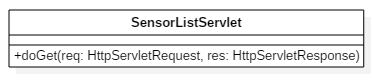
\includegraphics[width=0.6\linewidth]{images/database/classes/SensorListServlet}
\end{figure}
\subsubsection{Declaration}{
\begin{lstlisting}[frame=none]
public class SensorListServlet
 extends DatabaseConnection.HttpServlet\end{lstlisting}
\subsubsection{Constructor summary}{
\begin{verse}
\hyperlink{DatabaseConnection.SensorListServlet()}{{\bf SensorListServlet()}} Default constructor\\
\end{verse}
}
\subsubsection{Method summary}{
\begin{verse}
\hyperlink{DatabaseConnection.SensorListServlet.doGet(HttpServletRequest, HttpServletResponse)}{{\bf doGet(HttpServletRequest, HttpServletResponse)}} This method calls the getSensors method of the Facade to get a list of Sensors that are in a certain cluster.\\
\end{verse}
}
\subsubsection{Constructors}{
\vskip -2em
\begin{itemize}
\item{
\index{SensorListServlet()}
\hypertarget{DatabaseConnection.SensorListServlet()}{{\bf  SensorListServlet}\\}
\begin{lstlisting}[frame=none]
public SensorListServlet()\end{lstlisting} %end signature
\begin{itemize}
\item{
{\bf  Description}

Default constructor
}
\end{itemize}
}%end item
\end{itemize}
}
\subsubsection{Methods}{
\vskip -2em
\begin{itemize}
\item{
\index{doGet(HttpServletRequest, HttpServletResponse)}
\hypertarget{DatabaseConnection.SensorListServlet.doGet(HttpServletRequest, HttpServletResponse)}{{\bf  doGet}\\}
\begin{lstlisting}[frame=none]
public void doGet(HttpServletRequest req,HttpServletResponse res)\end{lstlisting} %end signature
\begin{itemize}
\item{
{\bf  Description}

This method calls the getSensors method of the Facade to get a list of Sensors that are in a certain cluster.
}
\item{
{\bf  Parameters}
  \begin{itemize}
   \item{
\texttt{req} -- An HttpServletRequest object that contains the request the client has made of the servlet.}
   \item{
\texttt{res} -- An HttpServletResponse object that contains the response the servlet sends to the client.}
  \end{itemize}
}%end item
\end{itemize}
}%end item
\end{itemize}
}
\subsubsection{Members inherited from class HttpServlet }{
\texttt{DatabaseConnection.HttpServlet} {\small
\refdefined{DatabaseConnection.HttpServlet}}
{\small

\vskip -2em
\begin{itemize}
\item{\vskip -1.5ex
\texttt{public void {\bf  doGet}(\texttt{HttpServletRequest} {\bf  req},
\texttt{HttpServletResponse} {\bf  res})
}%end signature
}%end item
\end{itemize}
}
}
\subsection{\label{DatabaseConnection.SensorMaintainer}Class SensorMaintainer}{
\hypertarget{DatabaseConnection.SensorMaintainer}{}\vskip .1in
This class maintains the list of sensors saved in the StorageSolution.\vskip .1in
\begin{figure}[!hbp]
	\centering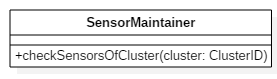
\includegraphics[width=0.4\linewidth]{images/database/classes/SensorMaintainer}
\end{figure}
\subsubsection{Declaration}{
\begin{lstlisting}[frame=none]
public class SensorMaintainer
 extends DatabaseConnection.Maintainer\end{lstlisting}
\subsubsection{Constructor summary}{
\begin{verse}
\hyperlink{DatabaseConnection.SensorMaintainer()}{{\bf SensorMaintainer()}} Default constructor\\
\end{verse}
}
\subsubsection{Method summary}{
\begin{verse}
\hyperlink{DatabaseConnection.SensorMaintainer.checkSensorsOfCluster(DatabaseConnection.ClusterID)}{{\bf checkSensorsOfCluster(ClusterID)}} This method checks if the sensors registered to the given cluster are up to date.\\
\end{verse}
}
\subsubsection{Constructors}{
\vskip -2em
\begin{itemize}
\item{
\index{SensorMaintainer()}
\hypertarget{DatabaseConnection.SensorMaintainer()}{{\bf  SensorMaintainer}\\}
\begin{lstlisting}[frame=none]
public SensorMaintainer()\end{lstlisting} %end signature
\begin{itemize}
\item{
{\bf  Description}

Default constructor
}
\end{itemize}
}%end item
\end{itemize}
}
\subsubsection{Methods}{
\vskip -2em
\begin{itemize}
\item{
\index{checkSensorsOfCluster(ClusterID)}
\hypertarget{DatabaseConnection.SensorMaintainer.checkSensorsOfCluster(DatabaseConnection.ClusterID)}{{\bf  checkSensorsOfCluster}\\}
\begin{lstlisting}[frame=none]
public void checkSensorsOfCluster(ClusterID cluster)\end{lstlisting} %end signature
\begin{itemize}
\item{
{\bf  Description}

This method checks if the sensors registered to the given cluster are up to date. A sensor is up to date if data has been received from it in the last 24 hours. If this requirement is not met, the sensor is deleted from the database.
}
\item{
{\bf  Parameters}
  \begin{itemize}
   \item{
\texttt{cluster} -- The cluster to check.}
  \end{itemize}
}%end item
\end{itemize}
}%end item
\end{itemize}
}
}
\subsection{\label{DatabaseConnection.ZoomLevel}Class ZoomLevel}{
\hypertarget{DatabaseConnection.ZoomLevel}{}\vskip .1in
This class describes a zoom level for the map.\vskip .1in
\begin{figure}[!hbp]
	\centering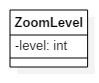
\includegraphics[width=0.2\linewidth]{images/database/classes/ZoomLevel}
\end{figure}
\subsubsection{Declaration}{
\begin{lstlisting}[frame=none]
public class ZoomLevel
 extends java.lang.Object\end{lstlisting}
\subsubsection{Constructor summary}{
\begin{verse}
\hyperlink{DatabaseConnection.ZoomLevel()}{{\bf ZoomLevel()}} Default constructor\\
\end{verse}
}
\subsubsection{Constructors}{
\vskip -2em
\begin{itemize}
\item{
\index{ZoomLevel()}
\hypertarget{DatabaseConnection.ZoomLevel()}{{\bf  ZoomLevel}\\}
\begin{lstlisting}[frame=none]
public ZoomLevel()\end{lstlisting} %end signature
\begin{itemize}
\item{
{\bf  Description}

Default constructor
}
\end{itemize}
}%end item
\end{itemize}
}
}
}

	\chapter{Graphite}
\begin{figure}[!htp]
	\centering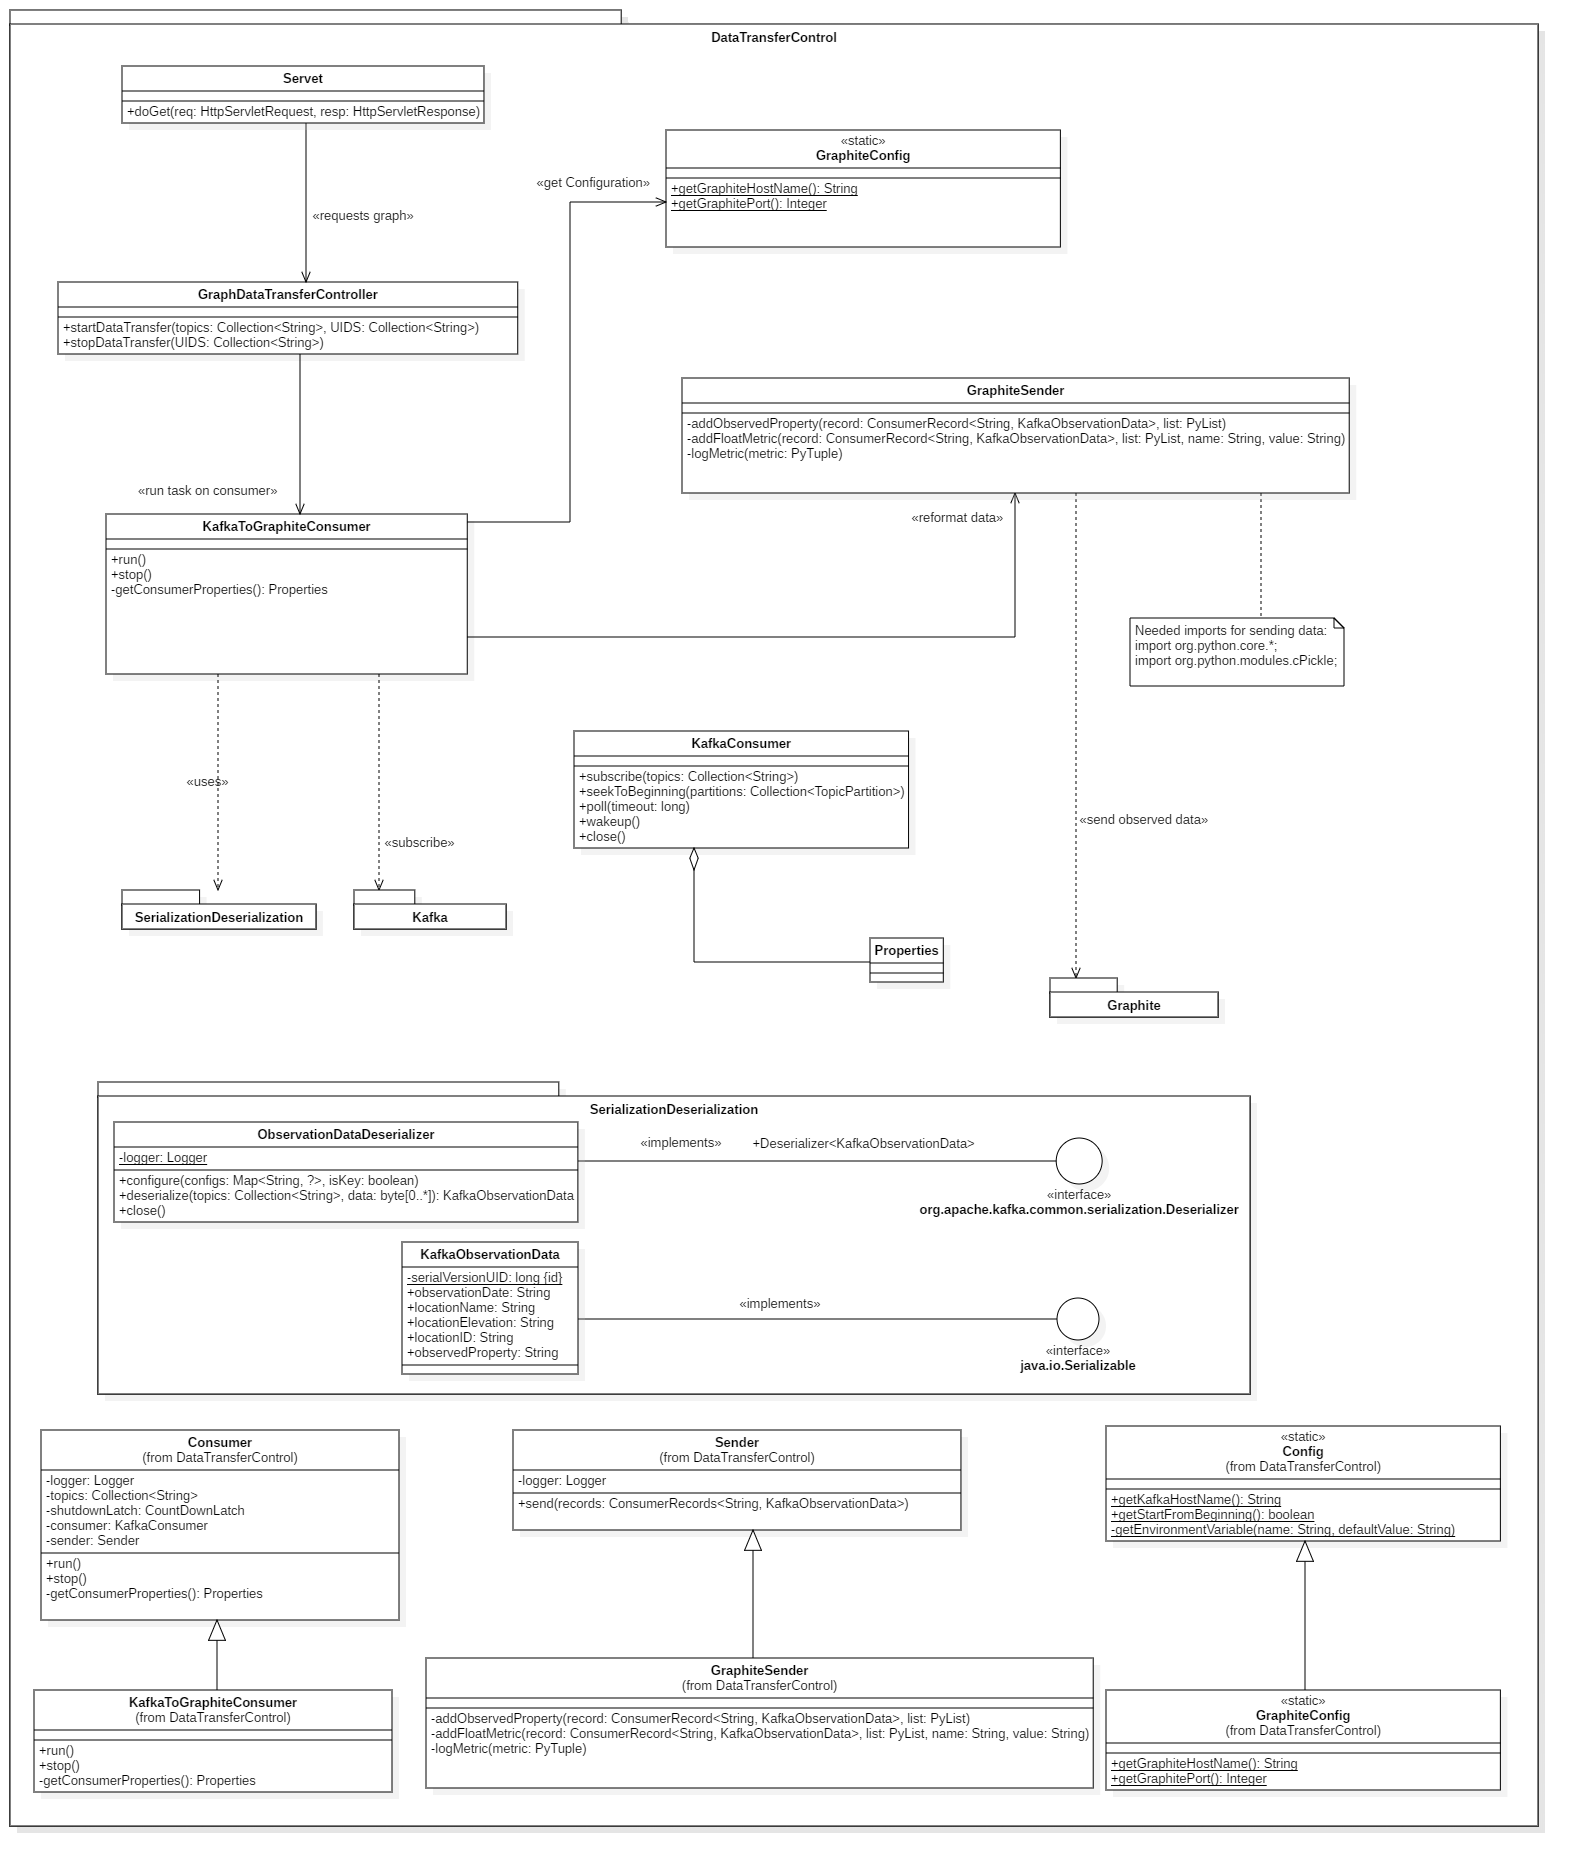
\includegraphics[width=\linewidth]{images/graphite/graphiteClassDiagram}
	\caption{Klassendiagramm Graphite}
\end{figure}
\section{Package DataTransferControl}{
\label{DataTransferControl}\hypertarget{DataTransferControl}{}
\hskip -.05in
\hbox to \hsize{\textit{ Package Contents\hfil Page}}
\vskip .13in
\hbox{{\bf  Classes}}
\entityintro{Collection}{DataTransferControl.Collection}{A Collection that stores multiple objects of one type}
\entityintro{Config}{DataTransferControl.Config}{The specified configuration-object that stores all needed configurations for the connection from Kafka to another specified component}
\entityintro{Consumer}{DataTransferControl.Consumer}{Consumes data from Kafka}
\entityintro{ConsumerRecord}{DataTransferControl.ConsumerRecord}{One single record of data from Kafka}
\entityintro{ConsumerRecords}{DataTransferControl.ConsumerRecords}{Multiple records of data from Kafka}
\entityintro{GraphDataTransferController}{DataTransferControl.GraphDataTransferController}{The Control-Unit in charge of creating and destroying KafkaToGraphiteConsumer as well as passing on the users request.}
\entityintro{GraphiteConfig}{DataTransferControl.GraphiteConfig}{The specified configuration-object that stores all needed configurations for the connection from Kafka to Graphite}
\entityintro{GraphiteSender}{DataTransferControl.GraphiteSender}{Reformats the data and sends it to Graphite}
\entityintro{KafkaConsumer}{DataTransferControl.KafkaConsumer}{The Kafka Consumer is described in Apache-Kafka and will only be included in this diagram for a better understanding of the required functionality.}
\entityintro{KafkaToGraphiteConsumer}{DataTransferControl.KafkaToGraphiteConsumer}{Receives the data from Kafka and sends it to Graphite}
\entityintro{Properties}{DataTransferControl.Properties}{The Properties of the KafkaConsumer, using Java.Util.Properties}
\entityintro{Sender}{DataTransferControl.Sender}{Reformats the data and sends it to another component}
\entityintro{Servet}{DataTransferControl.Servet}{A Servlet, which accepts the user-requests from the webinterface and passes them on to the responsible structures}
\vskip .1in
\vskip .1in
\subsection{\label{DataTransferControl.Collection}Class Collection}{
\hypertarget{DataTransferControl.Collection}{}\vskip .1in 
A Collection that stores multiple objects of one type\vskip .1in 
\subsubsection{Declaration}{
\begin{lstlisting}[frame=none]
public class Collection
 extends java.lang.Object\end{lstlisting}
\subsubsection{Constructor summary}{
\begin{verse}
\hyperlink{DataTransferControl.Collection()}{{\bf Collection()}} Default constructor\\
\end{verse}
}
\subsubsection{Constructors}{
\vskip -2em
\begin{itemize}
\item{ 
\index{Collection()}
\hypertarget{DataTransferControl.Collection()}{{\bf  Collection}\\}
\begin{lstlisting}[frame=none]
public Collection()\end{lstlisting} %end signature
\begin{itemize}
\item{
{\bf  Description}

Default constructor
}
\end{itemize}
}%end item
\end{itemize}
}
}
\subsection{\label{DataTransferControl.Config}Class Config}{
\hypertarget{DataTransferControl.Config}{}\vskip .1in 
The specified configuration-object that stores all needed configurations for the connection from Kafka to another specified component\vskip .1in 
\begin{figure}[!htp]
	\centering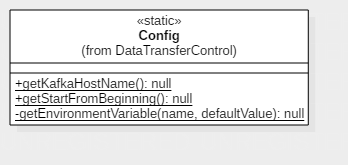
\includegraphics[width=0.4\linewidth]{images/graphite/classes/ClassConfig}
\end{figure} 
\subsubsection{Declaration}{
\begin{lstlisting}[frame=none]
public class Config
 extends java.lang.Object\end{lstlisting}
\subsubsection{All known subclasses}{GraphiteConfig\small{\refdefined{DataTransferControl.GraphiteConfig}}}
\subsubsection{Constructor summary}{
\begin{verse}
\hyperlink{DataTransferControl.Config()}{{\bf Config()}} Default constructor\\
\end{verse}
}
\subsubsection{Method summary}{
\begin{verse}
\hyperlink{DataTransferControl.Config.getKafkaHostName()}{{\bf getKafkaHostName()}} Gets the Kafka-host-name\\
\hyperlink{DataTransferControl.Config.getStartFromBeginning()}{{\bf getStartFromBeginning()}} Returns whether a start from the beginning is required\\
\end{verse}
}
\subsubsection{Constructors}{
\vskip -2em
\begin{itemize}
\item{ 
\index{Config()}
\hypertarget{DataTransferControl.Config()}{{\bf  Config}\\}
\begin{lstlisting}[frame=none]
public Config()\end{lstlisting} %end signature
\begin{itemize}
\item{
{\bf  Description}

Default constructor
}
\end{itemize}
}%end item
\end{itemize}
}
\subsubsection{Methods}{
\vskip -2em
\begin{itemize}
\item{ 
\index{getKafkaHostName()}
\hypertarget{DataTransferControl.Config.getKafkaHostName()}{{\bf  getKafkaHostName}\\}
\begin{lstlisting}[frame=none]
public static java.lang.String getKafkaHostName()\end{lstlisting} %end signature
\begin{itemize}
\item{
{\bf  Description}

Gets the Kafka-host-name
}
\item{{\bf  Returns} -- 
The host-name of Kafka 
}%end item
\end{itemize}
}%end item
\item{ 
\index{getStartFromBeginning()}
\hypertarget{DataTransferControl.Config.getStartFromBeginning()}{{\bf  getStartFromBeginning}\\}
\begin{lstlisting}[frame=none]
public static boolean getStartFromBeginning()\end{lstlisting} %end signature
\begin{itemize}
\item{
{\bf  Description}

Returns whether a start from the beginning is required
}
\item{{\bf  Returns} -- 
Tells us whether a start from the beginning is required 
}%end item
\end{itemize}
}%end item
\end{itemize}
}
}
\newpage
\subsection{\label{DataTransferControl.Consumer}Class Consumer}{
\hypertarget{DataTransferControl.Consumer}{}\vskip .1in 
Consumes data from Kafka\vskip .1in 
\begin{figure}[!htp]
	\centering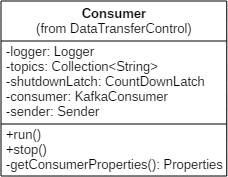
\includegraphics[width=0.3\linewidth]{images/graphite/classes/ClassConsumer}
\end{figure} 
\subsubsection{Declaration}{
\begin{lstlisting}[frame=none]
public class Consumer
 extends java.lang.Object\end{lstlisting}
\subsubsection{All known subclasses}{KafkaToGraphiteConsumer\small{\refdefined{DataTransferControl.KafkaToGraphiteConsumer}}}
\subsubsection{Constructor summary}{
\begin{verse}
\hyperlink{DataTransferControl.Consumer()}{{\bf Consumer()}} Default constructor\\
\end{verse}
}
\subsubsection{Method summary}{
\begin{verse}
\hyperlink{DataTransferControl.Consumer.run()}{{\bf run()}} Starts the transferring-process\\
\hyperlink{DataTransferControl.Consumer.stop()}{{\bf stop()}} Stops the transferring-process\\
\end{verse}
}
\subsubsection{Constructors}{
\vskip -2em
\begin{itemize}
\item{ 
\index{Consumer()}
\hypertarget{DataTransferControl.Consumer()}{{\bf  Consumer}\\}
\begin{lstlisting}[frame=none]
public Consumer()\end{lstlisting} %end signature
\begin{itemize}
\item{
{\bf  Description}

Default constructor
}
\end{itemize}
}%end item
\end{itemize}
}
\subsubsection{Methods}{
\vskip -2em
\begin{itemize}
\item{ 
\index{run()}
\hypertarget{DataTransferControl.Consumer.run()}{{\bf  run}\\}
\begin{lstlisting}[frame=none]
public void run()\end{lstlisting} %end signature
\begin{itemize}
\item{
{\bf  Description}

Starts the transferring-process
}
\end{itemize}
}%end item
\item{ 
\index{stop()}
\hypertarget{DataTransferControl.Consumer.stop()}{{\bf  stop}\\}
\begin{lstlisting}[frame=none]
public void stop()\end{lstlisting} %end signature
\begin{itemize}
\item{
{\bf  Description}

Stops the transferring-process
}
\end{itemize}
}%end item
\end{itemize}
}
}
\subsection{\label{DataTransferControl.ConsumerRecord}Class ConsumerRecord}{
\hypertarget{DataTransferControl.ConsumerRecord}{}\vskip .1in 
One single record of data from Kafka\vskip .1in 
\begin{figure}[!htp]
	\centering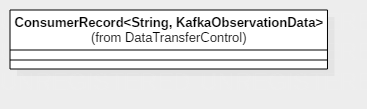
\includegraphics[width=0.2\linewidth]{images/graphite/classes/ClassConsumerRecord}
\end{figure} 
\subsubsection{Declaration}{
\begin{lstlisting}[frame=none]
public class ConsumerRecord
 extends java.lang.Object\end{lstlisting}
\subsubsection{Constructor summary}{
\begin{verse}
\hyperlink{DataTransferControl.ConsumerRecord()}{{\bf ConsumerRecord()}} Default constructor\\
\end{verse}
}
\subsubsection{Constructors}{
\vskip -2em
\begin{itemize}
\item{ 
\index{ConsumerRecord()}
\hypertarget{DataTransferControl.ConsumerRecord()}{{\bf  ConsumerRecord}\\}
\begin{lstlisting}[frame=none]
public ConsumerRecord()\end{lstlisting} %end signature
\begin{itemize}
\item{
{\bf  Description}

Default constructor
}
\end{itemize}
}%end item
\end{itemize}
}
}
\subsection{\label{DataTransferControl.ConsumerRecords}Class ConsumerRecords}{
\hypertarget{DataTransferControl.ConsumerRecords}{}\vskip .1in 
Multiple records of data from Kafka\vskip .1in 
\begin{figure}[!htp]
	\centering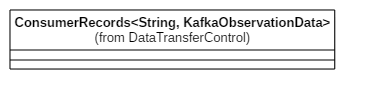
\includegraphics[width=0.2\linewidth]{images/graphite/classes/ClassConsumerRecords}
\end{figure} 
\subsubsection{Declaration}{
\begin{lstlisting}[frame=none]
public class ConsumerRecords
 extends java.lang.Object\end{lstlisting}
\subsubsection{Constructor summary}{
\begin{verse}
\hyperlink{DataTransferControl.ConsumerRecords()}{{\bf ConsumerRecords()}} Default constructor\\
\end{verse}
}
\subsubsection{Constructors}{
\vskip -2em
\begin{itemize}
\item{ 
\index{ConsumerRecords()}
\hypertarget{DataTransferControl.ConsumerRecords()}{{\bf  ConsumerRecords}\\}
\begin{lstlisting}[frame=none]
public ConsumerRecords()\end{lstlisting} %end signature
\begin{itemize}
\item{
{\bf  Description}

Default constructor
}
\end{itemize}
}%end item
\end{itemize}
}
}
\subsection{\label{DataTransferControl.GraphDataTransferController}Class GraphDataTransferController}{
\hypertarget{DataTransferControl.GraphDataTransferController}{}\vskip .1in 
The Control-Unit in charge of creating and destroying KafkaToGraphiteConsumer as well as passing on the users request.\vskip .1in 
\begin{figure}[!htp]
	\centering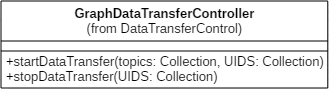
\includegraphics[width=0.6\linewidth]{images/graphite/classes/ClassGraphDataTransferController}
\end{figure} 
\subsubsection{Declaration}{
\begin{lstlisting}[frame=none]
public class GraphDataTransferController
 extends java.lang.Object\end{lstlisting}
\subsubsection{Constructor summary}{
\begin{verse}
\hyperlink{DataTransferControl.GraphDataTransferController()}{{\bf GraphDataTransferController()}} Default constructor\\
\end{verse}
}
\subsubsection{Method summary}{
\begin{verse}
\hyperlink{DataTransferControl.GraphDataTransferController.startDataTransfer(<any>, <any>)}{{\bf startDataTransfer(, )}} Starts data-transfer\\
\hyperlink{DataTransferControl.GraphDataTransferController.stopDataTransfer(<any>)}{{\bf stopDataTransfer()}} Stoppt den Datentransfer.\\
\end{verse}
}
\subsubsection{Constructors}{
\vskip -2em
\begin{itemize}
\item{ 
\index{GraphDataTransferController()}
\hypertarget{DataTransferControl.GraphDataTransferController()}{{\bf  GraphDataTransferController}\\}
\begin{lstlisting}[frame=none]
public GraphDataTransferController()\end{lstlisting} %end signature
\begin{itemize}
\item{
{\bf  Description}

Default constructor
}
\end{itemize}
}%end item
\end{itemize}
}
\subsubsection{Methods}{
\vskip -2em
\begin{itemize}
\item{ 
\index{startDataTransfer(, )}
\hypertarget{DataTransferControl.GraphDataTransferController.startDataTransfer(<any>, <any>)}{{\bf  startDataTransfer}\\}
\begin{lstlisting}[frame=none]
public void startDataTransfer(Collection<String> topics,Collection<String> UIDS)\end{lstlisting} %end signature
\begin{itemize}
\item{
{\bf  Description}

Starts data-transfer
}
\item{
{\bf  Parameters}
  \begin{itemize}
   \item{
\texttt{topics} -- Kafka-Topics that should be subscribed}
   \item{
\texttt{UIDS} -- The unique identifiers, that tell us which data should be transfered. Everything else will be ignored.}
  \end{itemize}
}%end item
\end{itemize}
}%end item
\item{ 
\index{stopDataTransfer()}
\hypertarget{DataTransferControl.GraphDataTransferController.stopDataTransfer(<any>)}{{\bf  stopDataTransfer}\\}
\begin{lstlisting}[frame=none]
public void stopDataTransfer(Collection<String> UIDS)\end{lstlisting} %end signature
\begin{itemize}
\item{
{\bf  Description}

Stoppt den Datentransfer.
}
\item{
{\bf  Parameters}
  \begin{itemize}
   \item{
\texttt{UIDS} -- The unique identifiers, that tell us which data should no longer be transfered. Everything else will be ignored.}
  \end{itemize}
}%end item
\end{itemize}
}%end item
\end{itemize}
}
}
\newpage
\subsection{\label{DataTransferControl.GraphiteConfig}Class GraphiteConfig}{
\hypertarget{DataTransferControl.GraphiteConfig}{}\vskip .1in 
The specified configuration-object that stores all needed configurations for the connection from Kafka to Graphite\vskip .1in 
\begin{figure}[!htp]
	\centering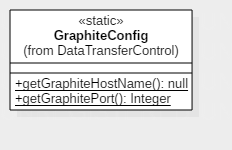
\includegraphics[width=0.25\linewidth]{images/graphite/classes/ClassGraphiteConfig}
\end{figure} 
\subsubsection{Declaration}{
\begin{lstlisting}[frame=none]
public class GraphiteConfig
 extends DataTransferControl.Config\end{lstlisting}
\subsubsection{Constructor summary}{
\begin{verse}
\hyperlink{DataTransferControl.GraphiteConfig()}{{\bf GraphiteConfig()}} Default constructor\\
\end{verse}
}
\subsubsection{Method summary}{
\begin{verse}
\hyperlink{DataTransferControl.GraphiteConfig.getGraphiteHostName()}{{\bf getGraphiteHostName()}} Returns the host-name of Graphite\\
\hyperlink{DataTransferControl.GraphiteConfig.getGraphitePort()}{{\bf getGraphitePort()}} Returns the port of the Graphite-connection\\
\end{verse}
}
\subsubsection{Constructors}{
\vskip -2em
\begin{itemize}
\item{ 
\index{GraphiteConfig()}
\hypertarget{DataTransferControl.GraphiteConfig()}{{\bf  GraphiteConfig}\\}
\begin{lstlisting}[frame=none]
public GraphiteConfig()\end{lstlisting} %end signature
\begin{itemize}
\item{
{\bf  Description}

Default constructor
}
\end{itemize}
}%end item
\end{itemize}
}
\subsubsection{Methods}{
\vskip -2em
\begin{itemize}
\item{ 
\index{getGraphiteHostName()}
\hypertarget{DataTransferControl.GraphiteConfig.getGraphiteHostName()}{{\bf  getGraphiteHostName}\\}
\begin{lstlisting}[frame=none]
public static java.lang.String getGraphiteHostName()\end{lstlisting} %end signature
\begin{itemize}
\item{
{\bf  Description}

Returns the host-name of Graphite
}
\item{{\bf  Returns} -- 
The Graphite-host-name 
}%end item
\end{itemize}
}%end item
\item{ 
\index{getGraphitePort()}
\hypertarget{DataTransferControl.GraphiteConfig.getGraphitePort()}{{\bf  getGraphitePort}\\}
\begin{lstlisting}[frame=none]
public static java.lang.Integer getGraphitePort()\end{lstlisting} %end signature
\begin{itemize}
\item{
{\bf  Description}

Returns the port of the Graphite-connection
}
\item{{\bf  Returns} -- 
The port of the Graphite-connection 
}%end item
\end{itemize}
}%end item
\end{itemize}
}
\subsubsection{Members inherited from class Config }{
\texttt{DataTransferControl.Config} {\small 
\refdefined{DataTransferControl.Config}}
{\small 

\vskip -2em
\begin{itemize}
\item{\vskip -1.5ex 
\texttt{public static String {\bf  getKafkaHostName}()
}%end signature
}%end item
\item{\vskip -1.5ex 
\texttt{public static boolean {\bf  getStartFromBeginning}()
}%end signature
}%end item
\end{itemize}
}
}
\subsection{\label{DataTransferControl.GraphiteSender}Class GraphiteSender}{
\hypertarget{DataTransferControl.GraphiteSender}{}\vskip .1in 
Reformats the data and sends it to Graphite\vskip .1in 
\begin{figure}[!htp]
	\centering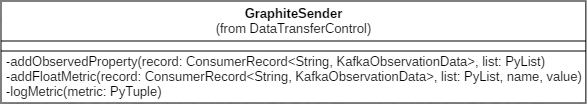
\includegraphics[width=0.8\linewidth]{images/graphite/classes/ClassGraphiteSender}
\end{figure} 
\subsubsection{Declaration}{
\begin{lstlisting}[frame=none]
public class GraphiteSender
 extends DataTransferControl.Sender\end{lstlisting}
\subsubsection{Constructor summary}{
\begin{verse}
\hyperlink{DataTransferControl.GraphiteSender()}{{\bf GraphiteSender()}} Default constructor\\
\end{verse}
}
\subsubsection{Constructors}{
\vskip -2em
\begin{itemize}
\item{ 
\index{GraphiteSender()}
\hypertarget{DataTransferControl.GraphiteSender()}{{\bf  GraphiteSender}\\}
\begin{lstlisting}[frame=none]
public GraphiteSender()\end{lstlisting} %end signature
\begin{itemize}
\item{
{\bf  Description}

Default constructor
}
\end{itemize}
}%end item
\end{itemize}
}
\subsubsection{Members inherited from class Sender }{
\texttt{DataTransferControl.Sender} {\small 
\refdefined{DataTransferControl.Sender}}
{\small 

\vskip -2em
\begin{itemize}
\item{\vskip -1.5ex 
\texttt{public void {\bf  send}(\texttt{} {\bf  records})
}%end signature
}%end item
\end{itemize}
}
}
\subsection{\label{DataTransferControl.KafkaConsumer}Class KafkaConsumer}{
\hypertarget{DataTransferControl.KafkaConsumer}{}\vskip .1in 
The Kafka Consumer is described in Apache-Kafka and will only be included in this diagram for a better understanding of the required functionality.\vskip .1in 
\begin{figure}[!htp]
	\centering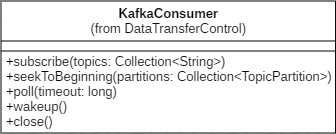
\includegraphics[width=0.4\linewidth]{images/graphite/classes/ClassKafkaConsumer}
\end{figure} 
\subsubsection{Declaration}{
\begin{lstlisting}[frame=none]
public class KafkaConsumer
 extends java.lang.Object\end{lstlisting}
\subsubsection{Constructor summary}{
\begin{verse}
\hyperlink{DataTransferControl.KafkaConsumer()}{{\bf KafkaConsumer()}} Default constructor\\
\end{verse}
}
\subsubsection{Method summary}{
\begin{verse}
\hyperlink{DataTransferControl.KafkaConsumer.close()}{{\bf close()}} Closes the KafkaConsumer\\
\hyperlink{DataTransferControl.KafkaConsumer.poll(long)}{{\bf poll(long)}} Gathers the data\\
\hyperlink{DataTransferControl.KafkaConsumer.seekToBeginning(<any>)}{{\bf seekToBeginning()}} Jumps to the beginning of an existing record\\
\hyperlink{DataTransferControl.KafkaConsumer.subscribe(<any>)}{{\bf subscribe()}} The Consumer subscribes Kafka-Topics.\\
\hyperlink{DataTransferControl.KafkaConsumer.wakeup()}{{\bf wakeup()}} Wakes up the KafkaConsumer, which then stops any current requests.\\
\end{verse}
}
\subsubsection{Constructors}{
\vskip -2em
\begin{itemize}
\item{ 
\index{KafkaConsumer()}
\hypertarget{DataTransferControl.KafkaConsumer()}{{\bf  KafkaConsumer}\\}
\begin{lstlisting}[frame=none]
public KafkaConsumer()\end{lstlisting} %end signature
\begin{itemize}
\item{
{\bf  Description}

Default constructor
}
\end{itemize}
}%end item
\end{itemize}
}
\subsubsection{Methods}{
\vskip -2em
\begin{itemize}
\item{ 
\index{close()}
\hypertarget{DataTransferControl.KafkaConsumer.close()}{{\bf  close}\\}
\begin{lstlisting}[frame=none]
public void close()\end{lstlisting} %end signature
\begin{itemize}
\item{
{\bf  Description}

Closes the KafkaConsumer
}
\end{itemize}
}%end item
\item{ 
\index{poll(long)}
\hypertarget{DataTransferControl.KafkaConsumer.poll(long)}{{\bf  poll}\\}
\begin{lstlisting}[frame=none]
public void poll(long timeout)\end{lstlisting} %end signature
\begin{itemize}
\item{
{\bf  Description}

Gathers the data
}
\item{
{\bf  Parameters}
  \begin{itemize}
   \item{
\texttt{timeout} -- A timeframe, limiting the longest possible duration of the poll request}
  \end{itemize}
}%end item
\end{itemize}
}%end item
\item{ 
\index{seekToBeginning()}
\hypertarget{DataTransferControl.KafkaConsumer.seekToBeginning(<any>)}{{\bf  seekToBeginning}\\}
\begin{lstlisting}[frame=none]
public void seekToBeginning(Collection<TopicPartition> partitions)\end{lstlisting} %end signature
\begin{itemize}
\item{
{\bf  Description}

Jumps to the beginning of an existing record
}
\item{
{\bf  Parameters}
  \begin{itemize}
   \item{
\texttt{partitions} -- Kafka-Partitions}
  \end{itemize}
}%end item
\end{itemize}
}%end item
\item{ 
\index{subscribe()}
\hypertarget{DataTransferControl.KafkaConsumer.subscribe(<any>)}{{\bf  subscribe}\\}
\begin{lstlisting}[frame=none]
public void subscribe(Collection<String> topics)\end{lstlisting} %end signature
\begin{itemize}
\item{
{\bf  Description}

The Consumer subscribes Kafka-Topics.
}
\item{
{\bf  Parameters}
  \begin{itemize}
   \item{
\texttt{topics} -- Kafka-Topics that should be subscribed}
  \end{itemize}
}%end item
\end{itemize}
}%end item
\item{ 
\index{wakeup()}
\hypertarget{DataTransferControl.KafkaConsumer.wakeup()}{{\bf  wakeup}\\}
\begin{lstlisting}[frame=none]
public void wakeup()\end{lstlisting} %end signature
\begin{itemize}
\item{
{\bf  Description}

Wakes up the KafkaConsumer, which then stops any current requests. Useful to limit polls in general.
}
\end{itemize}
}%end item
\end{itemize}
}
}
\subsection{\label{DataTransferControl.KafkaToGraphiteConsumer}Class KafkaToGraphiteConsumer}{
\hypertarget{DataTransferControl.KafkaToGraphiteConsumer}{}\vskip .1in 
Receives the data from Kafka and sends it to Graphite\vskip .1in 
\begin{figure}[!htp]
	\centering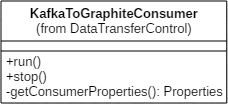
\includegraphics[width=0.3\linewidth]{images/graphite/classes/ClassKafkaToGraphiteConsumer}
\end{figure} 
\subsubsection{Declaration}{
\begin{lstlisting}[frame=none]
public class KafkaToGraphiteConsumer
 extends DataTransferControl.Consumer\end{lstlisting}
\subsubsection{Constructor summary}{
\begin{verse}
\hyperlink{DataTransferControl.KafkaToGraphiteConsumer()}{{\bf KafkaToGraphiteConsumer()}} Default constructor\\
\end{verse}
}
\subsubsection{Method summary}{
\begin{verse}
\hyperlink{DataTransferControl.KafkaToGraphiteConsumer.run()}{{\bf run()}} Starts the process of consumation and readying the sender object\\
\hyperlink{DataTransferControl.KafkaToGraphiteConsumer.stop()}{{\bf stop()}} Starts the process\\
\end{verse}
}
\subsubsection{Constructors}{
\vskip -2em
\begin{itemize}
\item{ 
\index{KafkaToGraphiteConsumer()}
\hypertarget{DataTransferControl.KafkaToGraphiteConsumer()}{{\bf  KafkaToGraphiteConsumer}\\}
\begin{lstlisting}[frame=none]
public KafkaToGraphiteConsumer()\end{lstlisting} %end signature
\begin{itemize}
\item{
{\bf  Description}

Default constructor
}
\end{itemize}
}%end item
\end{itemize}
}
\subsubsection{Methods}{
\vskip -2em
\begin{itemize}
\item{ 
\index{run()}
\hypertarget{DataTransferControl.KafkaToGraphiteConsumer.run()}{{\bf  run}\\}
\begin{lstlisting}[frame=none]
public void run()\end{lstlisting} %end signature
\begin{itemize}
\item{
{\bf  Description}

Starts the process of consumation and readying the sender object
}
\end{itemize}
}%end item
\item{ 
\index{stop()}
\hypertarget{DataTransferControl.KafkaToGraphiteConsumer.stop()}{{\bf  stop}\\}
\begin{lstlisting}[frame=none]
public void stop()\end{lstlisting} %end signature
\begin{itemize}
\item{
{\bf  Description}

Starts the process
}
\end{itemize}
}%end item
\end{itemize}
}
\subsubsection{Members inherited from class Consumer }{
\texttt{DataTransferControl.Consumer} {\small 
\refdefined{DataTransferControl.Consumer}}
{\small 

\vskip -2em
\begin{itemize}
\item{\vskip -1.5ex 
\texttt{public void {\bf  run}()
}%end signature
}%end item
\item{\vskip -1.5ex 
\texttt{public void {\bf  stop}()
}%end signature
}%end item
\end{itemize}
}
}
\subsection{\label{DataTransferControl.Properties}Class Properties}{
\hypertarget{DataTransferControl.Properties}{}\vskip .1in 
The Properties of the KafkaConsumer, using Java.Util.Properties\vskip .1in 
\begin{figure}[!htp]
	\centering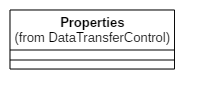
\includegraphics[width=0.25\linewidth]{images/graphite/classes/ClassProperties}
\end{figure} 
\subsubsection{Declaration}{
\begin{lstlisting}[frame=none]
public class Properties
 extends java.lang.Object\end{lstlisting}
\subsubsection{Constructor summary}{
\begin{verse}
\hyperlink{DataTransferControl.Properties()}{{\bf Properties()}} Default constructor\\
\end{verse}
}
\subsubsection{Constructors}{
\vskip -2em
\begin{itemize}
\item{ 
\index{Properties()}
\hypertarget{DataTransferControl.Properties()}{{\bf  Properties}\\}
\begin{lstlisting}[frame=none]
public Properties()\end{lstlisting} %end signature
\begin{itemize}
\item{
{\bf  Description}

Default constructor
}
\end{itemize}
}%end item
\end{itemize}
}
}
\newpage
\subsection{\label{DataTransferControl.Sender}Class Sender}{
\hypertarget{DataTransferControl.Sender}{}\vskip .1in 
Reformats the data and sends it to another component\vskip .1in 
\begin{figure}[!htp]
	\centering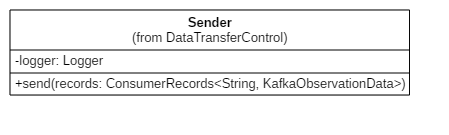
\includegraphics[width=0.6\linewidth]{images/graphite/classes/ClassSender}
\end{figure} 
\subsubsection{Declaration}{
\begin{lstlisting}[frame=none]
public class Sender
 extends java.lang.Object\end{lstlisting}
\subsubsection{All known subclasses}{GraphiteSender\small{\refdefined{DataTransferControl.GraphiteSender}}}
\subsubsection{Constructor summary}{
\begin{verse}
\hyperlink{DataTransferControl.Sender()}{{\bf Sender()}} Default constructor\\
\end{verse}
}
\subsubsection{Method summary}{
\begin{verse}
\hyperlink{DataTransferControl.Sender.send(<any>)}{{\bf send()}} Sends the resulting data to the specified component\\
\end{verse}
}
\subsubsection{Constructors}{
\vskip -2em
\begin{itemize}
\item{ 
\index{Sender()}
\hypertarget{DataTransferControl.Sender()}{{\bf  Sender}\\}
\begin{lstlisting}[frame=none]
public Sender()\end{lstlisting} %end signature
\begin{itemize}
\item{
{\bf  Description}

Default constructor
}
\end{itemize}
}%end item
\end{itemize}
}
\subsubsection{Methods}{
\vskip -2em
\begin{itemize}
\item{ 
\index{send()}
\hypertarget{DataTransferControl.Sender.send(<any>)}{{\bf  send}\\}
\begin{lstlisting}[frame=none]
public void send(ConsumerRecords<String, KafkaObservationData> records)\end{lstlisting} %end signature
\begin{itemize}
\item{
{\bf  Description}

Sends the resulting data to the specified component
}
\item{
{\bf  Parameters}
  \begin{itemize}
   \item{
\texttt{records} -- Multiple records of data from Kafka}
  \end{itemize}
}%end item
\end{itemize}
}%end item
\end{itemize}
}
}
\subsection{\label{DataTransferControl.Servet}Class Servlet}{
\hypertarget{DataTransferControl.Servet}{}\vskip .1in 
A Servlet, which accepts the user-requests from the webinterface and passes them on to the responsible structures\vskip .1in
\begin{figure}[!htp]
	\centering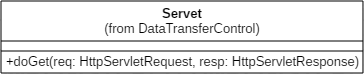
\includegraphics[width=0.5\linewidth]{images/graphite/classes/ClassServlet}
\end{figure} 
\subsubsection{Declaration}{
\begin{lstlisting}[frame=none]
public class Servet
 extends java.lang.Object\end{lstlisting}
\subsubsection{Constructor summary}{
\begin{verse}
\hyperlink{DataTransferControl.Servet()}{{\bf Servet()}} Default constructor\\
\end{verse}
}
\subsubsection{Method summary}{
\begin{verse}
\hyperlink{DataTransferControl.Servet.doGet(HttpServletRequest, HttpServletResponse)}{{\bf doGet(HttpServletRequest, HttpServletResponse)}} Receives the information of the data, that will be send back\\
\end{verse}
}
\subsubsection{Constructors}{
\vskip -2em
\begin{itemize}
\item{ 
\index{Servet()}
\hypertarget{DataTransferControl.Servet()}{{\bf  Servet}\\}
\begin{lstlisting}[frame=none]
public Servet()\end{lstlisting} %end signature
\begin{itemize}
\item{
{\bf  Description}

Default constructor
}
\end{itemize}
}%end item
\end{itemize}
}
\subsubsection{Methods}{
\vskip -2em
\begin{itemize}
\item{ 
\index{doGet(HttpServletRequest, HttpServletResponse)}
\hypertarget{DataTransferControl.Servet.doGet(HttpServletRequest, HttpServletResponse)}{{\bf  doGet}\\}
\begin{lstlisting}[frame=none]
public void doGet(HttpServletRequest req,HttpServletResponse resp)\end{lstlisting} %end signature
\begin{itemize}
\item{
{\bf  Description}

Receives the information of the data, that will be send back
}
\item{
{\bf  Parameters}
  \begin{itemize}
   \item{
\texttt{req} -- A http servlet request}
   \item{
\texttt{resp} -- A http servlet response}
  \end{itemize}
}%end item
\end{itemize}
}%end item
\end{itemize}
}
}
}
\section{Package DataTransferControl.SerializationDeserialization}{
\label{DataTransferControl.SerializationDeserialization}\hypertarget{DataTransferControl.SerializationDeserialization}{}
\hskip -.05in
\hbox to \hsize{\textit{ Package Contents\hfil Page}}
\vskip .13in
\hbox{{\bf  Classes}}
\entityintro{KafkaObservationData}{DataTransferControl.SerializationDeserialization.KafkaObservationData}{A serializable object that contains the observed data from kafka}
\entityintro{ObservationDataDeserializer}{DataTransferControl.SerializationDeserialization.ObservationDataDeserializer}{Deserializes KafkaObservationData objects}
\vskip .1in
\vskip .1in
\subsection{\label{DataTransferControl.SerializationDeserialization.KafkaObservationData}Class KafkaObservationData}{
\hypertarget{DataTransferControl.SerializationDeserialization.KafkaObservationData}{}\vskip .1in 
A serializable object that contains the observed data from kafka\vskip .1in 
\begin{figure}[!htp]
	\centering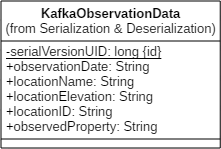
\includegraphics[width=0.3\linewidth]{images/graphite/classes/ClassKafkaObservationData}
\end{figure} 
\subsubsection{Declaration}{
\begin{lstlisting}[frame=none]
public class KafkaObservationData
 extends java.lang.Object implements java.io.Serializable\end{lstlisting}
\subsubsection{Field summary}{
\begin{verse}
\hyperlink{DataTransferControl.SerializationDeserialization.KafkaObservationData.locationElevation}{{\bf locationElevation}} The height of the observations location\\
\hyperlink{DataTransferControl.SerializationDeserialization.KafkaObservationData.locationID}{{\bf locationID}} The id of the observations location\\
\hyperlink{DataTransferControl.SerializationDeserialization.KafkaObservationData.locationName}{{\bf locationName}} The name of the observations location\\
\hyperlink{DataTransferControl.SerializationDeserialization.KafkaObservationData.observationDate}{{\bf observationDate}} The date of the observation\\
\hyperlink{DataTransferControl.SerializationDeserialization.KafkaObservationData.observedProperty}{{\bf observedProperty}} The observed property\\
\end{verse}
}
\subsubsection{Constructor summary}{
\begin{verse}
\hyperlink{DataTransferControl.SerializationDeserialization.KafkaObservationData()}{{\bf KafkaObservationData()}} Default constructor\\
\end{verse}
}
\subsubsection{Fields}{
\begin{itemize}
\item{
\index{observationDate}
\label{DataTransferControl.SerializationDeserialization.KafkaObservationData.observationDate}\hypertarget{DataTransferControl.SerializationDeserialization.KafkaObservationData.observationDate}{\texttt{public java.lang.String\ {\bf  observationDate}}
}
\begin{itemize}
\item{\vskip -.9ex 
The date of the observation}
\end{itemize}
}
\item{
\index{locationName}
\label{DataTransferControl.SerializationDeserialization.KafkaObservationData.locationName}\hypertarget{DataTransferControl.SerializationDeserialization.KafkaObservationData.locationName}{\texttt{public java.lang.String\ {\bf  locationName}}
}
\begin{itemize}
\item{\vskip -.9ex 
The name of the observations location}
\end{itemize}
}
\item{
\index{locationElevation}
\label{DataTransferControl.SerializationDeserialization.KafkaObservationData.locationElevation}\hypertarget{DataTransferControl.SerializationDeserialization.KafkaObservationData.locationElevation}{\texttt{public java.lang.String\ {\bf  locationElevation}}
}
\begin{itemize}
\item{\vskip -.9ex 
The height of the observations location}
\end{itemize}
}
\item{
\index{locationID}
\label{DataTransferControl.SerializationDeserialization.KafkaObservationData.locationID}\hypertarget{DataTransferControl.SerializationDeserialization.KafkaObservationData.locationID}{\texttt{public java.lang.String\ {\bf  locationID}}
}
\begin{itemize}
\item{\vskip -.9ex 
The id of the observations location}
\end{itemize}
}
\item{
\index{observedProperty}
\label{DataTransferControl.SerializationDeserialization.KafkaObservationData.observedProperty}\hypertarget{DataTransferControl.SerializationDeserialization.KafkaObservationData.observedProperty}{\texttt{public java.lang.String\ {\bf  observedProperty}}
}
\begin{itemize}
\item{\vskip -.9ex 
The observed property}
\end{itemize}
}
\end{itemize}
}
\subsubsection{Constructors}{
\vskip -2em
\begin{itemize}
\item{ 
\index{KafkaObservationData()}
\hypertarget{DataTransferControl.SerializationDeserialization.KafkaObservationData()}{{\bf  KafkaObservationData}\\}
\begin{lstlisting}[frame=none]
public KafkaObservationData()\end{lstlisting} %end signature
\begin{itemize}
\item{
{\bf  Description}

Default constructor
}
\end{itemize}
}%end item
\end{itemize}
}
}
\newpage
\subsection{\label{DataTransferControl.SerializationDeserialization.ObservationDataDeserializer}Class ObservationDataDeserializer}{
\hypertarget{DataTransferControl.SerializationDeserialization.ObservationDataDeserializer}{}\vskip .1in 
Deserializes KafkaObservationData objects\vskip .1in 
\begin{figure}[!htp]
	\centering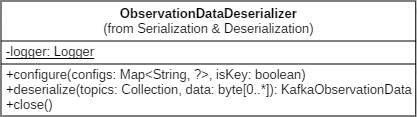
\includegraphics[width=0.65\linewidth]{images/graphite/classes/ClassObservationDataDeserializer}
\end{figure} 
\subsubsection{Declaration}{
\begin{lstlisting}[frame=none]
public class ObservationDataDeserializer
 extends java.lang.Object\end{lstlisting}
\subsubsection{Constructor summary}{
\begin{verse}
\hyperlink{DataTransferControl.SerializationDeserialization.ObservationDataDeserializer()}{{\bf ObservationDataDeserializer()}} Default constructor\\
\end{verse}
}
\subsubsection{Method summary}{
\begin{verse}
\hyperlink{DataTransferControl.SerializationDeserialization.ObservationDataDeserializer.close()}{{\bf close()}} Closes this object\\
\hyperlink{DataTransferControl.SerializationDeserialization.ObservationDataDeserializer.configure(java.util.Map, boolean)}{{\bf configure(Map, boolean)}} Configures the deserializer\\
\hyperlink{DataTransferControl.SerializationDeserialization.ObservationDataDeserializer.deserialize(java.util.Collection, java.util.Set)}{{\bf deserialize(Collection, Set)}} Deserializes an object\\
\end{verse}
}
\subsubsection{Constructors}{
\vskip -2em
\begin{itemize}
\item{ 
\index{ObservationDataDeserializer()}
\hypertarget{DataTransferControl.SerializationDeserialization.ObservationDataDeserializer()}{{\bf  ObservationDataDeserializer}\\}
\begin{lstlisting}[frame=none]
public ObservationDataDeserializer()\end{lstlisting} %end signature
\begin{itemize}
\item{
{\bf  Description}

Default constructor
}
\end{itemize}
}%end item
\end{itemize}
}
\subsubsection{Methods}{
\vskip -2em
\begin{itemize}
\item{ 
\index{close()}
\hypertarget{DataTransferControl.SerializationDeserialization.ObservationDataDeserializer.close()}{{\bf  close}\\}
\begin{lstlisting}[frame=none]
public void close()\end{lstlisting} %end signature
\begin{itemize}
\item{
{\bf  Description}

Closes this object
}
\end{itemize}
}%end item
\item{ 
\index{configure(Map, boolean)}
\hypertarget{DataTransferControl.SerializationDeserialization.ObservationDataDeserializer.configure(java.util.Map, boolean)}{{\bf  configure}\\}
\begin{lstlisting}[frame=none]
public void configure(java.util.Map configs,boolean isKey)\end{lstlisting} %end signature
\begin{itemize}
\item{
{\bf  Description}

Configures the deserializer
}
\item{
{\bf  Parameters}
  \begin{itemize}
   \item{
\texttt{configs} -- The Configuration}
   \item{
\texttt{isKey} -- A variable, telling us whether we want to configure the key or the value}
  \end{itemize}
}%end item
\end{itemize}
}%end item
\item{ 
\index{deserialize(Collection, Set)}
\hypertarget{DataTransferControl.SerializationDeserialization.ObservationDataDeserializer.deserialize(java.util.Collection, java.util.Set)}{{\bf  deserialize}\\}
\begin{lstlisting}[frame=none]
public KafkaObservationData deserialize(java.util.Collection topics,java.util.Set data)\end{lstlisting} %end signature
\begin{itemize}
\item{
{\bf  Description}

Deserializes an object
}
\item{
{\bf  Parameters}
  \begin{itemize}
   \item{
\texttt{topics} -- Kafka-Topics that should be subscribed}
   \item{
\texttt{data} -- These are our serialized bytes}
  \end{itemize}
}%end item
\item{{\bf  Returns} -- 
A serializable object that contains the observed data from kafka 
}%end item
\end{itemize}
}%end item
\end{itemize}
}
}
}

	\chapter{View}
\begin{figure}[!hbp]
	\centering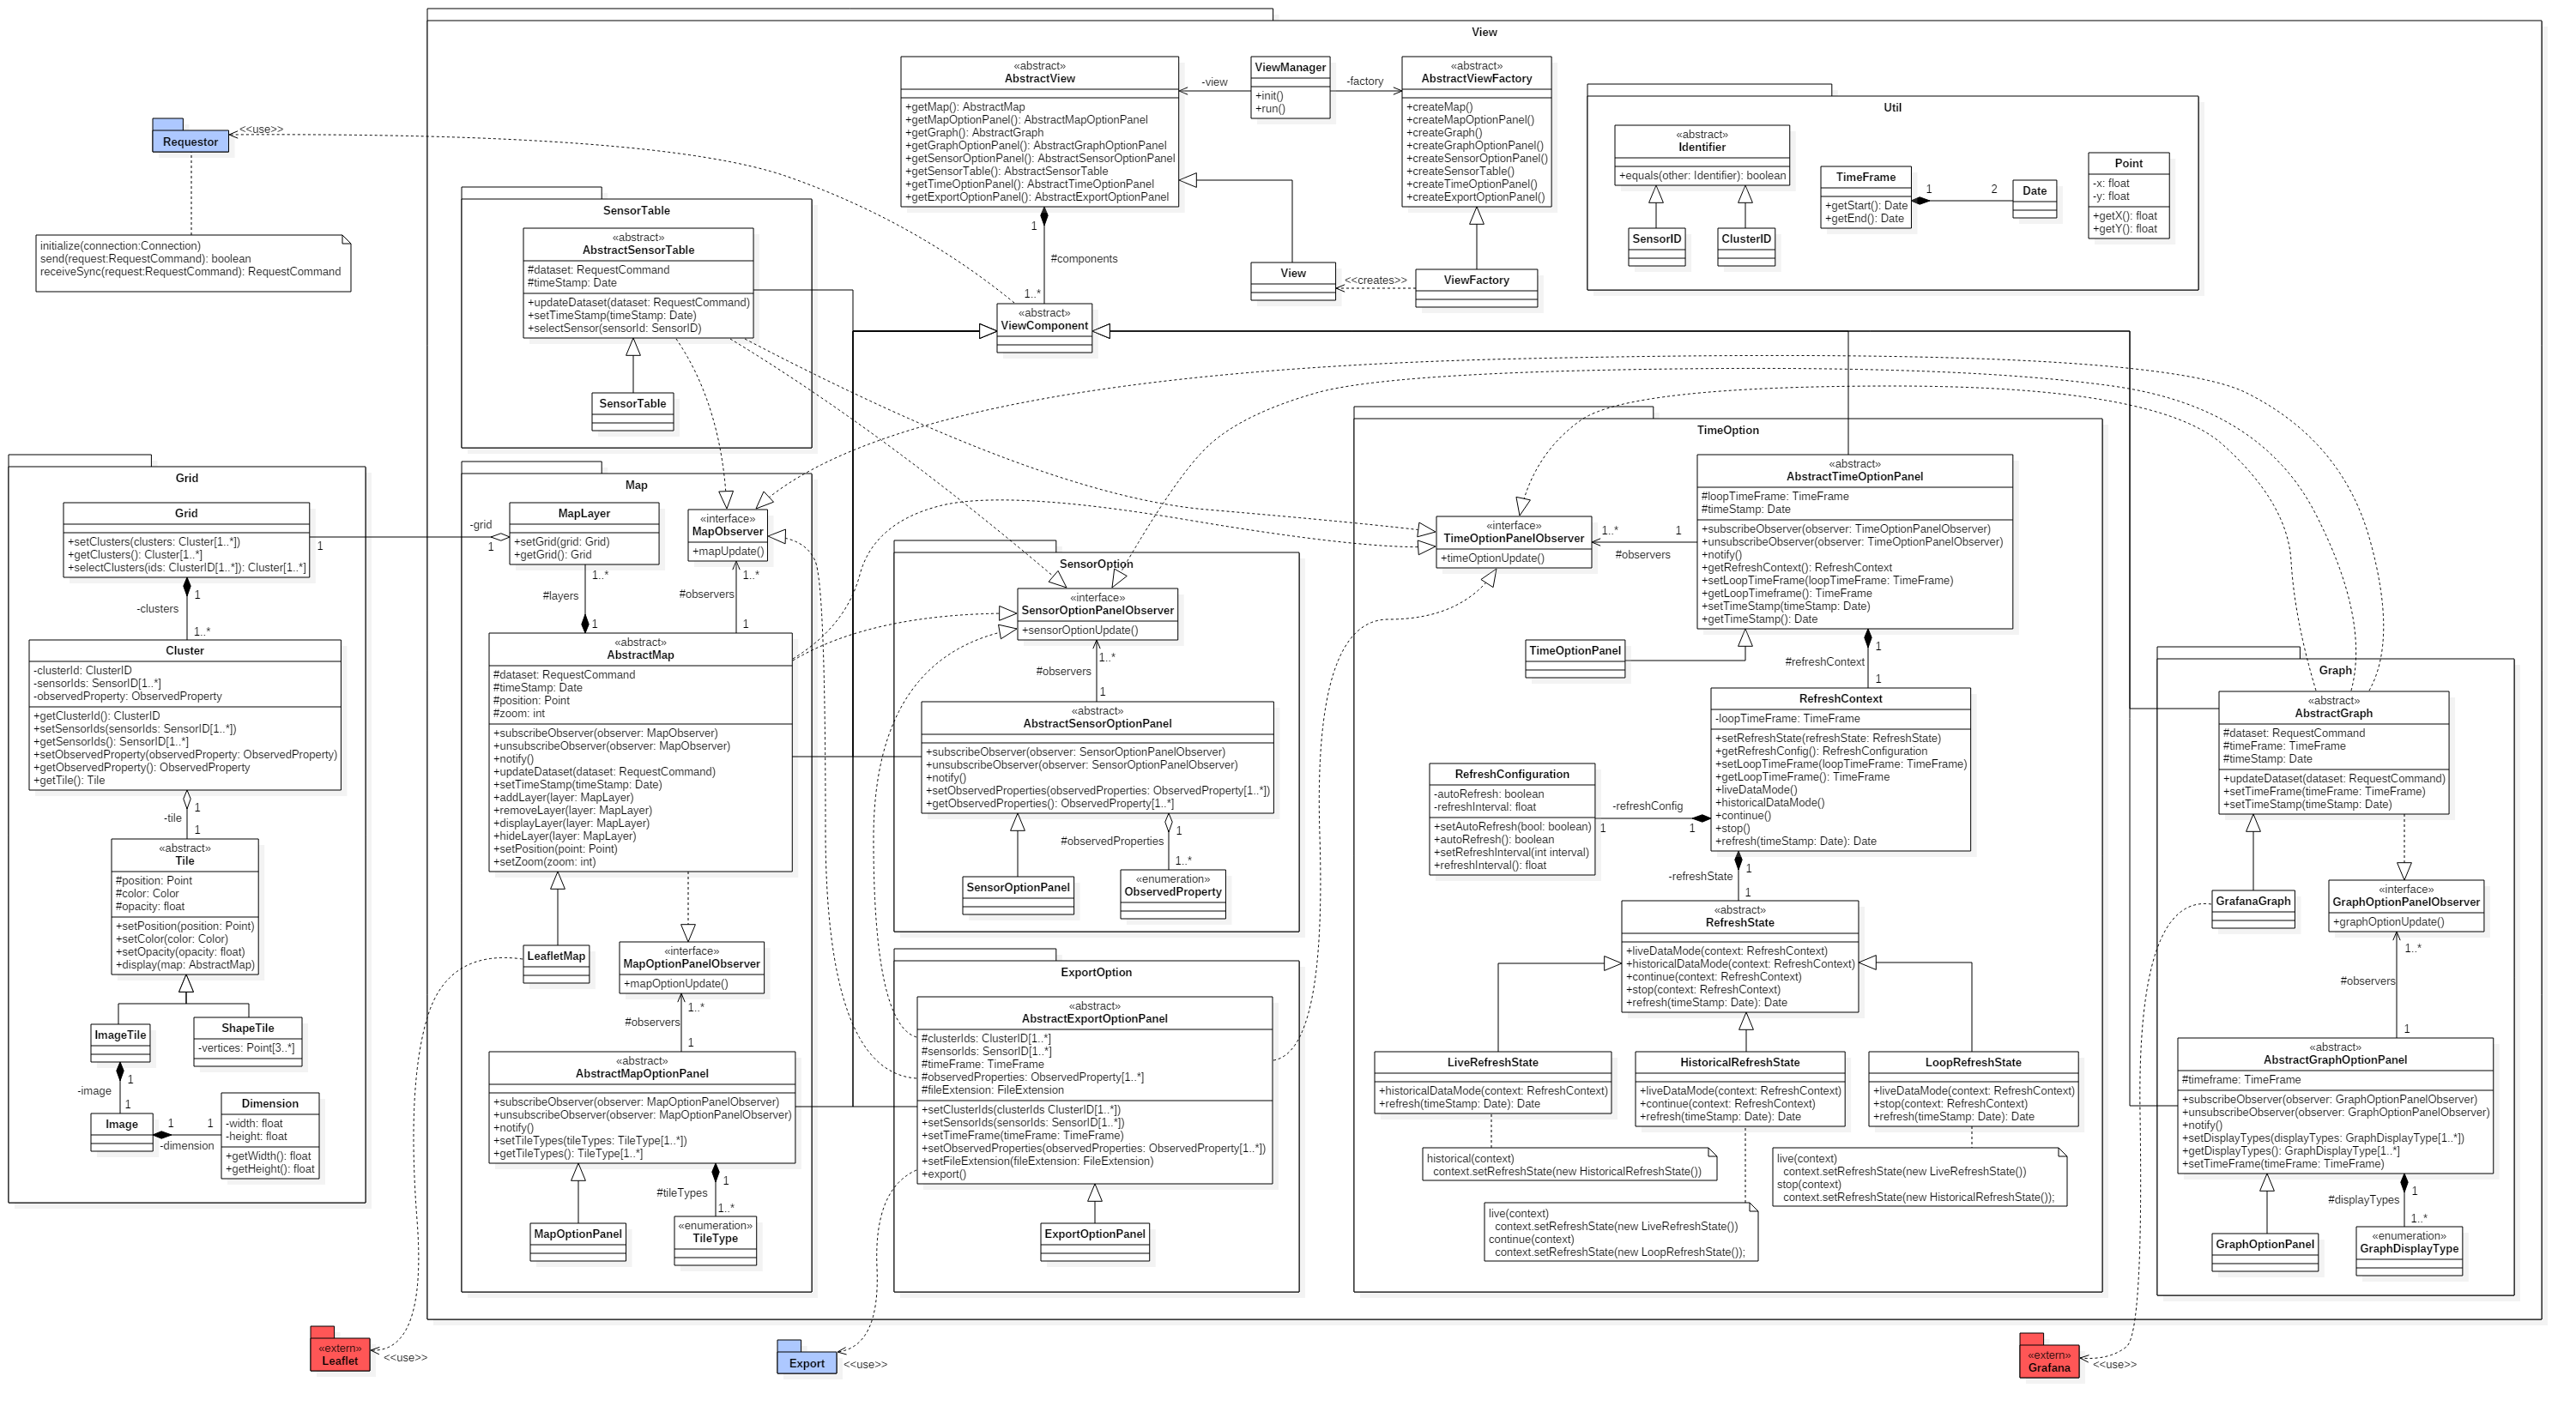
\includegraphics[width=1.25\linewidth,angle=90]{images/view/ViewClassDiagram}
	\caption{Klassendiagramm View}
\end{figure}
\section{Package Grid}{
\label{Grid}\hypertarget{Grid}{}
\hskip -.05in
\hbox to \hsize{\textit{ Package Contents\hfil Page}}
\vskip .13in
\hbox{{\bf  Classes}}
\entityintro{Cluster}{Grid.Cluster}{Encapsulates multiple sensors into a single object by using their specific SensorIDs and provides a graphical representation of their values average by using a Tile.}
\entityintro{Dimension}{Grid.Dimension}{Encapsulates the width and height of a component in float precision.}
\entityintro{Grid}{Grid.Grid}{Encapsulates multiple Clusters into a single object.}
\entityintro{Image}{Grid.Image}{Represents a graphical image.}
\entityintro{ImageTile}{Grid.ImageTile}{A Tile whose graphical representation consists of an image.}
\entityintro{ShapeTile}{Grid.ShapeTile}{A Tile whose graphical representation consists of a shape, specified by an array of vertices.}
\entityintro{Tile}{Grid.Tile}{A graphical structure that can be displayed on an AbstractMap.}
\vskip .1in
\vskip .1in
\newpage
\subsection{\label{Grid.Cluster}Class Cluster}{
\hypertarget{Grid.Cluster}{}\vskip .1in 
Encapsulates multiple sensors into a single object by using their specific SensorIDs and provides a graphical representation of their values average by using a Tile.\vskip .1in
\begin{figure}[!hbp]
	\centering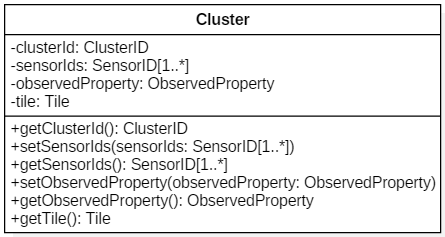
\includegraphics[width=0.5\linewidth]{images/view/classes/Cluster}
\end{figure} 
\subsubsection{Declaration}{
\begin{lstlisting}[frame=none]
public class Cluster
 extends java.lang.Object\end{lstlisting}
\subsubsection{Constructor summary}{
\begin{verse}
\hyperlink{Grid.Cluster()}{{\bf Cluster()}} Default constructor\\
\end{verse}
}
\subsubsection{Method summary}{
\begin{verse}
\hyperlink{Grid.Cluster.getClusterId()}{{\bf getClusterId()}} Get the ClusterID of this Cluster.\\
\hyperlink{Grid.Cluster.getObservedProperty()}{{\bf getObservedProperty()}} Get the ObservedProperty of this Cluster.\\
\hyperlink{Grid.Cluster.getSensorIds()}{{\bf getSensorIds()}} Get all SensorIDs of the sensors contained in this cluster.\\
\hyperlink{Grid.Cluster.getTile()}{{\bf getTile()}} Get the Tile of this Cluster.\\
\hyperlink{Grid.Cluster.setObservedProperty(ObservedProperty)}{{\bf setObservedProperty(ObservedProperty)}} Set the ObservedProperty of this Cluster.\\
\hyperlink{Grid.Cluster.setSensorIds(java.util.Set)}{{\bf setSensorIds(Set)}} Set the SensorIDs of the sensors contained in this cluster.\\
\end{verse}
}
\subsubsection{Constructors}{
\vskip -2em
\begin{itemize}
\item{ 
\index{Cluster()}
\hypertarget{Grid.Cluster()}{{\bf  Cluster}\\}
\begin{lstlisting}[frame=none]
public Cluster()\end{lstlisting} %end signature
\begin{itemize}
\item{
{\bf  Description}

Default constructor
}
\end{itemize}
}%end item
\end{itemize}
}
\subsubsection{Methods}{
\vskip -2em
\begin{itemize}
\item{ 
\index{getClusterId()}
\hypertarget{Grid.Cluster.getClusterId()}{{\bf  getClusterId}\\}
\begin{lstlisting}[frame=none]
public ClusterID getClusterId()\end{lstlisting} %end signature
\begin{itemize}
\item{
{\bf  Description}

Get the ClusterID of this Cluster.
}
\item{{\bf  Returns} -- 
the ClusterID of this Cluster. 
}%end item
\end{itemize}
}%end item
\item{ 
\index{getObservedProperty()}
\hypertarget{Grid.Cluster.getObservedProperty()}{{\bf  getObservedProperty}\\}
\begin{lstlisting}[frame=none]
public ObservedProperty getObservedProperty()\end{lstlisting} %end signature
\begin{itemize}
\item{
{\bf  Description}

Get the ObservedProperty of this Cluster.
}
\item{{\bf  Returns} -- 
the ObservedProperty of this Cluster. 
}%end item
\end{itemize}
}%end item
\item{ 
\index{getSensorIds()}
\hypertarget{Grid.Cluster.getSensorIds()}{{\bf  getSensorIds}\\}
\begin{lstlisting}[frame=none]
public java.util.Set getSensorIds()\end{lstlisting} %end signature
\begin{itemize}
\item{
{\bf  Description}

Get all SensorIDs of the sensors contained in this cluster.
}
\item{{\bf  Returns} -- 
all SensorIDs of the sensors contained in this cluster. 
}%end item
\end{itemize}
}%end item
\item{ 
\index{getTile()}
\hypertarget{Grid.Cluster.getTile()}{{\bf  getTile}\\}
\begin{lstlisting}[frame=none]
public Tile getTile()\end{lstlisting} %end signature
\begin{itemize}
\item{
{\bf  Description}

Get the Tile of this Cluster.
}
\item{{\bf  Returns} -- 
the Tile of this Cluster. 
}%end item
\end{itemize}
}%end item
\item{ 
\index{setObservedProperty(ObservedProperty)}
\hypertarget{Grid.Cluster.setObservedProperty(ObservedProperty)}{{\bf  setObservedProperty}\\}
\begin{lstlisting}[frame=none]
public void setObservedProperty(ObservedProperty observedProperty)\end{lstlisting} %end signature
\begin{itemize}
\item{
{\bf  Description}

Set the ObservedProperty of this Cluster.
}
\item{
{\bf  Parameters}
  \begin{itemize}
   \item{
\texttt{observedProperty} -- }
  \end{itemize}
}%end item
\end{itemize}
}%end item
\item{ 
\index{setSensorIds(Set)}
\hypertarget{Grid.Cluster.setSensorIds(java.util.Set)}{{\bf  setSensorIds}\\}
\begin{lstlisting}[frame=none]
public void setSensorIds(java.util.Set sensorIds)\end{lstlisting} %end signature
\begin{itemize}
\item{
{\bf  Description}

Set the SensorIDs of the sensors contained in this cluster.
}
\item{
{\bf  Parameters}
  \begin{itemize}
   \item{
\texttt{sensorIds} -- }
  \end{itemize}
}%end item
\end{itemize}
}%end item
\end{itemize}
}
}
\subsection{\label{Grid.Dimension}Class Dimension}{
\hypertarget{Grid.Dimension}{}\vskip .1in 
Encapsulates the width and height of a component in float precision.\vskip .1in
\begin{figure}[!hbp]
	\centering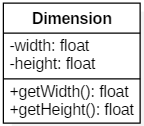
\includegraphics[width=0.5\linewidth]{images/view/classes/Dimension}
\end{figure} 
\subsubsection{Declaration}{
\begin{lstlisting}[frame=none]
public class Dimension
 extends java.lang.Object\end{lstlisting}
\subsubsection{Constructor summary}{
\begin{verse}
\hyperlink{Grid.Dimension()}{{\bf Dimension()}} Default constructor\\
\end{verse}
}
\subsubsection{Method summary}{
\begin{verse}
\hyperlink{Grid.Dimension.getHeight()}{{\bf getHeight()}} Get the height of this Dimension.\\
\hyperlink{Grid.Dimension.getWidth()}{{\bf getWidth()}} Get the width of this Dimension.\\
\end{verse}
}
\subsubsection{Constructors}{
\vskip -2em
\begin{itemize}
\item{ 
\index{Dimension()}
\hypertarget{Grid.Dimension()}{{\bf  Dimension}\\}
\begin{lstlisting}[frame=none]
public Dimension()\end{lstlisting} %end signature
\begin{itemize}
\item{
{\bf  Description}

Default constructor
}
\end{itemize}
}%end item
\end{itemize}
}
\subsubsection{Methods}{
\vskip -2em
\begin{itemize}
\item{ 
\index{getHeight()}
\hypertarget{Grid.Dimension.getHeight()}{{\bf  getHeight}\\}
\begin{lstlisting}[frame=none]
public float getHeight()\end{lstlisting} %end signature
\begin{itemize}
\item{
{\bf  Description}

Get the height of this Dimension.
}
\item{{\bf  Returns} -- 
the height of this Dimension. 
}%end item
\end{itemize}
}%end item
\item{ 
\index{getWidth()}
\hypertarget{Grid.Dimension.getWidth()}{{\bf  getWidth}\\}
\begin{lstlisting}[frame=none]
public float getWidth()\end{lstlisting} %end signature
\begin{itemize}
\item{
{\bf  Description}

Get the width of this Dimension.
}
\item{{\bf  Returns} -- 
the width of this Dimension. 
}%end item
\end{itemize}
}%end item
\end{itemize}
}
}
\subsection{\label{Grid.Grid}Class Grid}{
\hypertarget{Grid.Grid}{}\vskip .1in 
Encapsulates multiple Clusters into a single object.\vskip .1in 
\begin{figure}[!hbp]
	\centering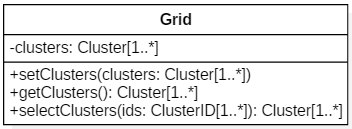
\includegraphics[width=0.5\linewidth]{images/view/classes/Grid}
\end{figure} 
\subsubsection{Declaration}{
\begin{lstlisting}[frame=none]
public class Grid
 extends java.lang.Object\end{lstlisting}
\subsubsection{Constructor summary}{
\begin{verse}
\hyperlink{Grid.Grid()}{{\bf Grid()}} Default constructor\\
\end{verse}
}
\subsubsection{Method summary}{
\begin{verse}
\hyperlink{Grid.Grid.getClusters()}{{\bf getClusters()}} Get all Clusters contained in this Grid.\\
\hyperlink{Grid.Grid.selectClusters(java.util.Set)}{{\bf selectClusters(Set)}} Select Clusters contained in this Grid by using their specific ClusterIDs.\\
\hyperlink{Grid.Grid.setClusters(java.util.Set)}{{\bf setClusters(Set)}} Set the Clusters contained in this Grid.\\
\end{verse}
}
\subsubsection{Constructors}{
\vskip -2em
\begin{itemize}
\item{ 
\index{Grid()}
\hypertarget{Grid.Grid()}{{\bf  Grid}\\}
\begin{lstlisting}[frame=none]
public Grid()\end{lstlisting} %end signature
\begin{itemize}
\item{
{\bf  Description}

Default constructor
}
\end{itemize}
}%end item
\end{itemize}
}
\subsubsection{Methods}{
\vskip -2em
\begin{itemize}
\item{ 
\index{getClusters()}
\hypertarget{Grid.Grid.getClusters()}{{\bf  getClusters}\\}
\begin{lstlisting}[frame=none]
public java.util.Set getClusters()\end{lstlisting} %end signature
\begin{itemize}
\item{
{\bf  Description}

Get all Clusters contained in this Grid.
}
\item{{\bf  Returns} -- 
all Clusters contained in this Grid. 
}%end item
\end{itemize}
}%end item
\item{ 
\index{selectClusters(Set)}
\hypertarget{Grid.Grid.selectClusters(java.util.Set)}{{\bf  selectClusters}\\}
\begin{lstlisting}[frame=none]
public java.util.Set selectClusters(java.util.Set ids)\end{lstlisting} %end signature
\begin{itemize}
\item{
{\bf  Description}

Select Clusters contained in this Grid by using their specific ClusterIDs.
}
\item{
{\bf  Parameters}
  \begin{itemize}
   \item{
\texttt{ids} -- }
  \end{itemize}
}%end item
\item{{\bf  Returns} -- 
selected Clusters contained in this Grid identified by their specific ClusterIDs. 
}%end item
\end{itemize}
}%end item
\item{ 
\index{setClusters(Set)}
\hypertarget{Grid.Grid.setClusters(java.util.Set)}{{\bf  setClusters}\\}
\begin{lstlisting}[frame=none]
public void setClusters(java.util.Set clusters)\end{lstlisting} %end signature
\begin{itemize}
\item{
{\bf  Description}

Set the Clusters contained in this Grid.
}
\item{
{\bf  Parameters}
  \begin{itemize}
   \item{
\texttt{clusters} -- }
  \end{itemize}
}%end item
\end{itemize}
}%end item
\end{itemize}
}
}
\subsection{\label{Grid.Image}Class Image}{
\hypertarget{Grid.Image}{}\vskip .1in 
Represents a graphical image.\vskip .1in
\begin{figure}[!hbp]
	\centering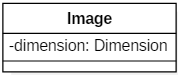
\includegraphics[width=0.5\linewidth]{images/view/classes/Image}
\end{figure} 
\subsubsection{Declaration}{
\begin{lstlisting}[frame=none]
public class Image
 extends java.lang.Object\end{lstlisting}
\subsubsection{Constructor summary}{
\begin{verse}
\hyperlink{Grid.Image()}{{\bf Image()}} Default constructor\\
\end{verse}
}
\subsubsection{Constructors}{
\vskip -2em
\begin{itemize}
\item{ 
\index{Image()}
\hypertarget{Grid.Image()}{{\bf  Image}\\}
\begin{lstlisting}[frame=none]
public Image()\end{lstlisting} %end signature
\begin{itemize}
\item{
{\bf  Description}

Default constructor
}
\end{itemize}
}%end item
\end{itemize}
}
}
\subsection{\label{Grid.ImageTile}Class ImageTile}{
\hypertarget{Grid.ImageTile}{}\vskip .1in 
A Tile whose graphical representation consists of an image.\vskip .1in 
\begin{figure}[!hbp]
	\centering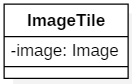
\includegraphics[width=0.5\linewidth]{images/view/classes/ImageTile}
\end{figure} 
\subsubsection{Declaration}{
\begin{lstlisting}[frame=none]
public class ImageTile
 extends Grid.Tile\end{lstlisting}
\subsubsection{Constructor summary}{
\begin{verse}
\hyperlink{Grid.ImageTile()}{{\bf ImageTile()}} Default constructor\\
\end{verse}
}
\subsubsection{Constructors}{
\vskip -2em
\begin{itemize}
\item{ 
\index{ImageTile()}
\hypertarget{Grid.ImageTile()}{{\bf  ImageTile}\\}
\begin{lstlisting}[frame=none]
public ImageTile()\end{lstlisting} %end signature
\begin{itemize}
\item{
{\bf  Description}

Default constructor
}
\end{itemize}
}%end item
\end{itemize}
}
\subsubsection{Members inherited from class Tile }{
\texttt{Grid.Tile} {\small 
\refdefined{Grid.Tile}}
{\small 

\vskip -2em
\begin{itemize}
\item{\vskip -1.5ex 
\texttt{protected {\bf  color}}%end signature
}%end item
\item{\vskip -1.5ex 
\texttt{public void {\bf  display}(\texttt{java.util.AbstractMap} {\bf  map})
}%end signature
}%end item
\item{\vskip -1.5ex 
\texttt{protected {\bf  opacity}}%end signature
}%end item
\item{\vskip -1.5ex 
\texttt{protected {\bf  position}}%end signature
}%end item
\item{\vskip -1.5ex 
\texttt{public void {\bf  setColor}(\texttt{Color} {\bf  color})
}%end signature
}%end item
\item{\vskip -1.5ex 
\texttt{public void {\bf  setOpacity}(\texttt{float} {\bf  opacity})
}%end signature
}%end item
\item{\vskip -1.5ex 
\texttt{public void {\bf  setPosition}(\texttt{Point} {\bf  position})
}%end signature
}%end item
\end{itemize}
}
}
\subsection{\label{Grid.ShapeTile}Class ShapeTile}{
\hypertarget{Grid.ShapeTile}{}\vskip .1in 
A Tile whose graphical representation consists of a shape, specified by an array of vertices.\vskip .1in
\begin{figure}[!hbp]
	\centering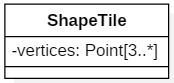
\includegraphics[width=0.5\linewidth]{images/view/classes/ShapeTile}
\end{figure} 
\subsubsection{Declaration}{
\begin{lstlisting}[frame=none]
public class ShapeTile
 extends Grid.Tile\end{lstlisting}
\subsubsection{Constructor summary}{
\begin{verse}
\hyperlink{Grid.ShapeTile()}{{\bf ShapeTile()}} Default constructor\\
\end{verse}
}
\subsubsection{Constructors}{
\vskip -2em
\begin{itemize}
\item{ 
\index{ShapeTile()}
\hypertarget{Grid.ShapeTile()}{{\bf  ShapeTile}\\}
\begin{lstlisting}[frame=none]
public ShapeTile()\end{lstlisting} %end signature
\begin{itemize}
\item{
{\bf  Description}

Default constructor
}
\end{itemize}
}%end item
\end{itemize}
}
\subsubsection{Members inherited from class Tile }{
\texttt{Grid.Tile} {\small 
\refdefined{Grid.Tile}}
{\small 

\vskip -2em
\begin{itemize}
\item{\vskip -1.5ex 
\texttt{protected {\bf  color}}%end signature
}%end item
\item{\vskip -1.5ex 
\texttt{public void {\bf  display}(\texttt{java.util.AbstractMap} {\bf  map})
}%end signature
}%end item
\item{\vskip -1.5ex 
\texttt{protected {\bf  opacity}}%end signature
}%end item
\item{\vskip -1.5ex 
\texttt{protected {\bf  position}}%end signature
}%end item
\item{\vskip -1.5ex 
\texttt{public void {\bf  setColor}(\texttt{Color} {\bf  color})
}%end signature
}%end item
\item{\vskip -1.5ex 
\texttt{public void {\bf  setOpacity}(\texttt{float} {\bf  opacity})
}%end signature
}%end item
\item{\vskip -1.5ex 
\texttt{public void {\bf  setPosition}(\texttt{Point} {\bf  position})
}%end signature
}%end item
\end{itemize}
}
}
\subsection{\label{Grid.Tile}Class Tile}{
\hypertarget{Grid.Tile}{}\vskip .1in 
A graphical structure that can be displayed on an AbstractMap.\vskip .1in 
\begin{figure}[!hbp]
	\centering\includegraphics[width=0.5\linewidth]{images/view/classes/Tile}
\end{figure} 
\subsubsection{Declaration}{
\begin{lstlisting}[frame=none]
public class Tile
 extends java.lang.Object\end{lstlisting}
\subsubsection{All known subclasses}{ShapeTile\small{\refdefined{Grid.ShapeTile}}, ImageTile\small{\refdefined{Grid.ImageTile}}}
\subsubsection{Field summary}{
\begin{verse}
\hyperlink{Grid.Tile.color}{{\bf color}} \\
\hyperlink{Grid.Tile.opacity}{{\bf opacity}} \\
\hyperlink{Grid.Tile.position}{{\bf position}} \\
\end{verse}
}
\subsubsection{Constructor summary}{
\begin{verse}
\hyperlink{Grid.Tile()}{{\bf Tile()}} Default constructor\\
\end{verse}
}
\subsubsection{Method summary}{
\begin{verse}
\hyperlink{Grid.Tile.display(java.util.AbstractMap)}{{\bf display(AbstractMap)}} Display this tile on the submitted map.\\
\hyperlink{Grid.Tile.setColor(Color)}{{\bf setColor(Color)}} Set the color of this Tile.\\
\hyperlink{Grid.Tile.setOpacity(float)}{{\bf setOpacity(float)}} Set the opacity of this Tile.\\
\hyperlink{Grid.Tile.setPosition(Point)}{{\bf setPosition(Point)}} Set the position of this Tile.\\
\end{verse}
}
\subsubsection{Fields}{
\begin{itemize}
\item{
\index{position}
\label{Grid.Tile.position}\hypertarget{Grid.Tile.position}{\texttt{protected Point\ {\bf  position}}
}
}
\item{
\index{color}
\label{Grid.Tile.color}\hypertarget{Grid.Tile.color}{\texttt{protected Color\ {\bf  color}}
}
}
\item{
\index{opacity}
\label{Grid.Tile.opacity}\hypertarget{Grid.Tile.opacity}{\texttt{protected float\ {\bf  opacity}}
}
}
\end{itemize}
}
\subsubsection{Constructors}{
\vskip -2em
\begin{itemize}
\item{ 
\index{Tile()}
\hypertarget{Grid.Tile()}{{\bf  Tile}\\}
\begin{lstlisting}[frame=none]
public Tile()\end{lstlisting} %end signature
\begin{itemize}
\item{
{\bf  Description}

Default constructor
}
\end{itemize}
}%end item
\end{itemize}
}
\subsubsection{Methods}{
\vskip -2em
\begin{itemize}
\item{ 
\index{display(AbstractMap)}
\hypertarget{Grid.Tile.display(java.util.AbstractMap)}{{\bf  display}\\}
\begin{lstlisting}[frame=none]
public void display(java.util.AbstractMap map)\end{lstlisting} %end signature
\begin{itemize}
\item{
{\bf  Description}

Display this tile on the submitted map.
}
\item{
{\bf  Parameters}
  \begin{itemize}
   \item{
\texttt{map} -- }
  \end{itemize}
}%end item
\end{itemize}
}%end item
\item{ 
\index{setColor(Color)}
\hypertarget{Grid.Tile.setColor(Color)}{{\bf  setColor}\\}
\begin{lstlisting}[frame=none]
public void setColor(Color color)\end{lstlisting} %end signature
\begin{itemize}
\item{
{\bf  Description}

Set the color of this Tile.
}
\item{
{\bf  Parameters}
  \begin{itemize}
   \item{
\texttt{color} -- }
  \end{itemize}
}%end item
\end{itemize}
}%end item
\item{ 
\index{setOpacity(float)}
\hypertarget{Grid.Tile.setOpacity(float)}{{\bf  setOpacity}\\}
\begin{lstlisting}[frame=none]
public void setOpacity(float opacity)\end{lstlisting} %end signature
\begin{itemize}
\item{
{\bf  Description}

Set the opacity of this Tile.
}
\item{
{\bf  Parameters}
  \begin{itemize}
   \item{
\texttt{opacity} -- }
  \end{itemize}
}%end item
\end{itemize}
}%end item
\item{ 
\index{setPosition(Point)}
\hypertarget{Grid.Tile.setPosition(Point)}{{\bf  setPosition}\\}
\begin{lstlisting}[frame=none]
public void setPosition(Point position)\end{lstlisting} %end signature
\begin{itemize}
\item{
{\bf  Description}

Set the position of this Tile.
}
\item{
{\bf  Parameters}
  \begin{itemize}
   \item{
\texttt{position} -- }
  \end{itemize}
}%end item
\end{itemize}
}%end item
\end{itemize}
}
}
}
\section{Package View}{
\label{View}\hypertarget{View}{}
\hskip -.05in
\hbox to \hsize{\textit{ Package Contents\hfil Page}}
\vskip .13in
\hbox{{\bf  Classes}}
\entityintro{AbstractView}{View.AbstractView}{Encapsulates all ViewComponents created by the AbstractViewFactory into a single object.}
\entityintro{AbstractViewFactory}{View.AbstractViewFactory}{A factory for the creation of a View.}
\entityintro{View}{View.View}{An implementation of AbstractView.}
\entityintro{ViewComponent}{View.ViewComponent}{A view component which the View is made up of.}
\entityintro{ViewFactory}{View.ViewFactory}{An Implementation of AbstractViewFactory.}
\entityintro{ViewManager}{View.ViewManager}{Initializes and runs the AbstractView.}
\vskip .1in
\vskip .1in
\subsection{\label{View.AbstractView}Class AbstractView}{
\hypertarget{View.AbstractView}{}\vskip .1in 
Encapsulates all ViewComponents created by the AbstractViewFactory into a single object.\vskip .1in 
\begin{figure}[!hbp]
	\centering\includegraphics[width=0.5\linewidth]{images/view/classes/AbstractView}
\end{figure} 
\subsubsection{Declaration}{
\begin{lstlisting}[frame=none]
public class AbstractView
 extends java.lang.Object\end{lstlisting}
\subsubsection{All known subclasses}{View\small{\refdefined{View.View}}}
\subsubsection{Constructor summary}{
\begin{verse}
\hyperlink{View.AbstractView()}{{\bf AbstractView()}} Default constructor\\
\end{verse}
}
\subsubsection{Method summary}{
\begin{verse}
\hyperlink{View.AbstractView.getExportOptionPanel()}{{\bf getExportOptionPanel()}} Get the AbstractExportOptionPanel.\\
\hyperlink{View.AbstractView.getGraph()}{{\bf getGraph()}} Get the AbstractGraph.\\
\hyperlink{View.AbstractView.getGraphOptionPanel()}{{\bf getGraphOptionPanel()}} Get the AbstractGraphOptionPanel.\\
\hyperlink{View.AbstractView.getMap()}{{\bf getMap()}} Get the AbstractMap.\\
\hyperlink{View.AbstractView.getMapOptionPanel()}{{\bf getMapOptionPanel()}} Get the AbstractMapOptionPanel.\\
\hyperlink{View.AbstractView.getSensorOptionPanel()}{{\bf getSensorOptionPanel()}} Get the AbstractSensorOptionPanel.\\
\hyperlink{View.AbstractView.getSensorTable()}{{\bf getSensorTable()}} Get the AbstractSensorTable.\\
\hyperlink{View.AbstractView.getTimeOptionPanel()}{{\bf getTimeOptionPanel()}} Get the AbstractTimeOptionPanel.\\
\end{verse}
}
\subsubsection{Constructors}{
\vskip -2em
\begin{itemize}
\item{ 
\index{AbstractView()}
\hypertarget{View.AbstractView()}{{\bf  AbstractView}\\}
\begin{lstlisting}[frame=none]
public AbstractView()\end{lstlisting} %end signature
\begin{itemize}
\item{
{\bf  Description}

Default constructor
}
\end{itemize}
}%end item
\end{itemize}
}
\subsubsection{Methods}{
\vskip -2em
\begin{itemize}
\item{ 
\index{getExportOptionPanel()}
\hypertarget{View.AbstractView.getExportOptionPanel()}{{\bf  getExportOptionPanel}\\}
\begin{lstlisting}[frame=none]
public AbstractExportOptionPanel getExportOptionPanel()\end{lstlisting} %end signature
\begin{itemize}
\item{
{\bf  Description}

Get the AbstractExportOptionPanel.
}
\item{{\bf  Returns} -- 
the AbstractExportOptionPanel. 
}%end item
\end{itemize}
}%end item
\item{ 
\index{getGraph()}
\hypertarget{View.AbstractView.getGraph()}{{\bf  getGraph}\\}
\begin{lstlisting}[frame=none]
public AbstractGraph getGraph()\end{lstlisting} %end signature
\begin{itemize}
\item{
{\bf  Description}

Get the AbstractGraph.
}
\item{{\bf  Returns} -- 
the AbstractGraph. 
}%end item
\end{itemize}
}%end item
\item{ 
\index{getGraphOptionPanel()}
\hypertarget{View.AbstractView.getGraphOptionPanel()}{{\bf  getGraphOptionPanel}\\}
\begin{lstlisting}[frame=none]
public AbstractGraphOptionPanel getGraphOptionPanel()\end{lstlisting} %end signature
\begin{itemize}
\item{
{\bf  Description}

Get the AbstractGraphOptionPanel.
}
\item{{\bf  Returns} -- 
the AbstractGraphOptionPanel. 
}%end item
\end{itemize}
}%end item
\item{ 
\index{getMap()}
\hypertarget{View.AbstractView.getMap()}{{\bf  getMap}\\}
\begin{lstlisting}[frame=none]
public java.util.AbstractMap getMap()\end{lstlisting} %end signature
\begin{itemize}
\item{
{\bf  Description}

Get the AbstractMap.
}
\item{{\bf  Returns} -- 
the AbstractMap. 
}%end item
\end{itemize}
}%end item
\item{ 
\index{getMapOptionPanel()}
\hypertarget{View.AbstractView.getMapOptionPanel()}{{\bf  getMapOptionPanel}\\}
\begin{lstlisting}[frame=none]
public AbstractMapOptionPanel getMapOptionPanel()\end{lstlisting} %end signature
\begin{itemize}
\item{
{\bf  Description}

Get the AbstractMapOptionPanel.
}
\item{{\bf  Returns} -- 
the AbstractMapOptionPanel. 
}%end item
\end{itemize}
}%end item
\item{ 
\index{getSensorOptionPanel()}
\hypertarget{View.AbstractView.getSensorOptionPanel()}{{\bf  getSensorOptionPanel}\\}
\begin{lstlisting}[frame=none]
public AbstractSensorOptionPanel getSensorOptionPanel()\end{lstlisting} %end signature
\begin{itemize}
\item{
{\bf  Description}

Get the AbstractSensorOptionPanel.
}
\item{{\bf  Returns} -- 
the AbstractSensorOptionPanel. 
}%end item
\end{itemize}
}%end item
\item{ 
\index{getSensorTable()}
\hypertarget{View.AbstractView.getSensorTable()}{{\bf  getSensorTable}\\}
\begin{lstlisting}[frame=none]
public AbstractSensorTable getSensorTable()\end{lstlisting} %end signature
\begin{itemize}
\item{
{\bf  Description}

Get the AbstractSensorTable.
}
\item{{\bf  Returns} -- 
the AbstractSensorTable. 
}%end item
\end{itemize}
}%end item
\item{ 
\index{getTimeOptionPanel()}
\hypertarget{View.AbstractView.getTimeOptionPanel()}{{\bf  getTimeOptionPanel}\\}
\begin{lstlisting}[frame=none]
public AbstractTimeOptionPanel getTimeOptionPanel()\end{lstlisting} %end signature
\begin{itemize}
\item{
{\bf  Description}

Get the AbstractTimeOptionPanel.
}
\item{{\bf  Returns} -- 
the AbstractTimeOptionPanel. 
}%end item
\end{itemize}
}%end item
\end{itemize}
}
}
\subsection{\label{View.AbstractViewFactory}Class AbstractViewFactory}{
\hypertarget{View.AbstractViewFactory}{}\vskip .1in 
A factory for the creation of a View.\vskip .1in 
\begin{figure}[!hbp]
	\centering\includegraphics[width=0.5\linewidth]{images/view/classes/AbstractViewFactory}
\end{figure} 
\subsubsection{Declaration}{
\begin{lstlisting}[frame=none]
public class AbstractViewFactory
 extends java.lang.Object\end{lstlisting}
\subsubsection{All known subclasses}{ViewFactory\small{\refdefined{View.ViewFactory}}}
\subsubsection{Constructor summary}{
\begin{verse}
\hyperlink{View.AbstractViewFactory()}{{\bf AbstractViewFactory()}} Default constructor\\
\end{verse}
}
\subsubsection{Method summary}{
\begin{verse}
\hyperlink{View.AbstractViewFactory.createExportOptionPanel()}{{\bf createExportOptionPanel()}} Create an AbstractExportOptionPanel.\\
\hyperlink{View.AbstractViewFactory.createGraph()}{{\bf createGraph()}} Create an AbstractGraph.\\
\hyperlink{View.AbstractViewFactory.createGraphOptionPanel()}{{\bf createGraphOptionPanel()}} Create an AbstractGraphOptionPanel.\\
\hyperlink{View.AbstractViewFactory.createMap()}{{\bf createMap()}} Create an AbstractMap.\\
\hyperlink{View.AbstractViewFactory.createMapOptionPanel()}{{\bf createMapOptionPanel()}} Create an AbstractMapOptionPanel.\\
\hyperlink{View.AbstractViewFactory.createSensorOptionPanel()}{{\bf createSensorOptionPanel()}} Create an AbstractSensorOptionPanel.\\
\hyperlink{View.AbstractViewFactory.createSensorTable()}{{\bf createSensorTable()}} Create an AbstractSensorTable.\\
\hyperlink{View.AbstractViewFactory.createTimeOptionPanel()}{{\bf createTimeOptionPanel()}} Create an AbstractTimeOptionPanel.\\
\end{verse}
}
\subsubsection{Constructors}{
\vskip -2em
\begin{itemize}
\item{ 
\index{AbstractViewFactory()}
\hypertarget{View.AbstractViewFactory()}{{\bf  AbstractViewFactory}\\}
\begin{lstlisting}[frame=none]
public AbstractViewFactory()\end{lstlisting} %end signature
\begin{itemize}
\item{
{\bf  Description}

Default constructor
}
\end{itemize}
}%end item
\end{itemize}
}
\subsubsection{Methods}{
\vskip -2em
\begin{itemize}
\item{ 
\index{createExportOptionPanel()}
\hypertarget{View.AbstractViewFactory.createExportOptionPanel()}{{\bf  createExportOptionPanel}\\}
\begin{lstlisting}[frame=none]
public void createExportOptionPanel()\end{lstlisting} %end signature
\begin{itemize}
\item{
{\bf  Description}

Create an AbstractExportOptionPanel.
}
\end{itemize}
}%end item
\item{ 
\index{createGraph()}
\hypertarget{View.AbstractViewFactory.createGraph()}{{\bf  createGraph}\\}
\begin{lstlisting}[frame=none]
public void createGraph()\end{lstlisting} %end signature
\begin{itemize}
\item{
{\bf  Description}

Create an AbstractGraph.
}
\end{itemize}
}%end item
\item{ 
\index{createGraphOptionPanel()}
\hypertarget{View.AbstractViewFactory.createGraphOptionPanel()}{{\bf  createGraphOptionPanel}\\}
\begin{lstlisting}[frame=none]
public void createGraphOptionPanel()\end{lstlisting} %end signature
\begin{itemize}
\item{
{\bf  Description}

Create an AbstractGraphOptionPanel.
}
\end{itemize}
}%end item
\item{ 
\index{createMap()}
\hypertarget{View.AbstractViewFactory.createMap()}{{\bf  createMap}\\}
\begin{lstlisting}[frame=none]
public void createMap()\end{lstlisting} %end signature
\begin{itemize}
\item{
{\bf  Description}

Create an AbstractMap.
}
\end{itemize}
}%end item
\item{ 
\index{createMapOptionPanel()}
\hypertarget{View.AbstractViewFactory.createMapOptionPanel()}{{\bf  createMapOptionPanel}\\}
\begin{lstlisting}[frame=none]
public void createMapOptionPanel()\end{lstlisting} %end signature
\begin{itemize}
\item{
{\bf  Description}

Create an AbstractMapOptionPanel.
}
\end{itemize}
}%end item
\item{ 
\index{createSensorOptionPanel()}
\hypertarget{View.AbstractViewFactory.createSensorOptionPanel()}{{\bf  createSensorOptionPanel}\\}
\begin{lstlisting}[frame=none]
public void createSensorOptionPanel()\end{lstlisting} %end signature
\begin{itemize}
\item{
{\bf  Description}

Create an AbstractSensorOptionPanel.
}
\end{itemize}
}%end item
\item{ 
\index{createSensorTable()}
\hypertarget{View.AbstractViewFactory.createSensorTable()}{{\bf  createSensorTable}\\}
\begin{lstlisting}[frame=none]
public void createSensorTable()\end{lstlisting} %end signature
\begin{itemize}
\item{
{\bf  Description}

Create an AbstractSensorTable.
}
\end{itemize}
}%end item
\item{ 
\index{createTimeOptionPanel()}
\hypertarget{View.AbstractViewFactory.createTimeOptionPanel()}{{\bf  createTimeOptionPanel}\\}
\begin{lstlisting}[frame=none]
public void createTimeOptionPanel()\end{lstlisting} %end signature
\begin{itemize}
\item{
{\bf  Description}

Create an AbstractTimeOptionPanel.
}
\end{itemize}
}%end item
\end{itemize}
}
}
\subsection{\label{View.View}Class View}{
\hypertarget{View.View}{}\vskip .1in 
An implementation of AbstractView.\vskip .1in 
\begin{figure}[!hbp]
	\centering\includegraphics[width=0.5\linewidth]{images/view/classes/View}
\end{figure} 
\subsubsection{Declaration}{
\begin{lstlisting}[frame=none]
public class View
 extends View.AbstractView\end{lstlisting}
\subsubsection{Constructor summary}{
\begin{verse}
\hyperlink{View.View()}{{\bf View()}} Default constructor\\
\end{verse}
}
\subsubsection{Constructors}{
\vskip -2em
\begin{itemize}
\item{ 
\index{View()}
\hypertarget{View.View()}{{\bf  View}\\}
\begin{lstlisting}[frame=none]
public View()\end{lstlisting} %end signature
\begin{itemize}
\item{
{\bf  Description}

Default constructor
}
\end{itemize}
}%end item
\end{itemize}
}
\subsubsection{Members inherited from class AbstractView }{
\texttt{View.AbstractView} {\small 
\refdefined{View.AbstractView}}
{\small 

\vskip -2em
\begin{itemize}
\item{\vskip -1.5ex 
\texttt{public AbstractExportOptionPanel {\bf  getExportOptionPanel}()
}%end signature
}%end item
\item{\vskip -1.5ex 
\texttt{public AbstractGraph {\bf  getGraph}()
}%end signature
}%end item
\item{\vskip -1.5ex 
\texttt{public AbstractGraphOptionPanel {\bf  getGraphOptionPanel}()
}%end signature
}%end item
\item{\vskip -1.5ex 
\texttt{public AbstractMap {\bf  getMap}()
}%end signature
}%end item
\item{\vskip -1.5ex 
\texttt{public AbstractMapOptionPanel {\bf  getMapOptionPanel}()
}%end signature
}%end item
\item{\vskip -1.5ex 
\texttt{public AbstractSensorOptionPanel {\bf  getSensorOptionPanel}()
}%end signature
}%end item
\item{\vskip -1.5ex 
\texttt{public AbstractSensorTable {\bf  getSensorTable}()
}%end signature
}%end item
\item{\vskip -1.5ex 
\texttt{public AbstractTimeOptionPanel {\bf  getTimeOptionPanel}()
}%end signature
}%end item
\end{itemize}
}
}
\subsection{\label{View.ViewComponent}Class ViewComponent}{
\hypertarget{View.ViewComponent}{}\vskip .1in 
A view component which the View is made up of.\vskip .1in 
\begin{figure}[!hbp]
	\centering\includegraphics[width=0.5\linewidth]{images/view/classes/ViewComponent}
\end{figure} 
\subsubsection{Declaration}{
\begin{lstlisting}[frame=none]
public class ViewComponent
 extends java.lang.Object\end{lstlisting}
\subsubsection{Constructor summary}{
\begin{verse}
\hyperlink{View.ViewComponent()}{{\bf ViewComponent()}} Default constructor\\
\end{verse}
}
\subsubsection{Constructors}{
\vskip -2em
\begin{itemize}
\item{ 
\index{ViewComponent()}
\hypertarget{View.ViewComponent()}{{\bf  ViewComponent}\\}
\begin{lstlisting}[frame=none]
public ViewComponent()\end{lstlisting} %end signature
\begin{itemize}
\item{
{\bf  Description}

Default constructor
}
\end{itemize}
}%end item
\end{itemize}
}
}
\subsection{\label{View.ViewFactory}Class ViewFactory}{
\hypertarget{View.ViewFactory}{}\vskip .1in 
An Implementation of AbstractViewFactory.\vskip .1in 
\begin{figure}[!hbp]
	\centering\includegraphics[width=0.5\linewidth]{images/view/classes/ViewFactory}
\end{figure} 
\subsubsection{Declaration}{
\begin{lstlisting}[frame=none]
public class ViewFactory
 extends View.AbstractViewFactory\end{lstlisting}
\subsubsection{Constructor summary}{
\begin{verse}
\hyperlink{View.ViewFactory()}{{\bf ViewFactory()}} Default constructor\\
\end{verse}
}
\subsubsection{Constructors}{
\vskip -2em
\begin{itemize}
\item{ 
\index{ViewFactory()}
\hypertarget{View.ViewFactory()}{{\bf  ViewFactory}\\}
\begin{lstlisting}[frame=none]
public ViewFactory()\end{lstlisting} %end signature
\begin{itemize}
\item{
{\bf  Description}

Default constructor
}
\end{itemize}
}%end item
\end{itemize}
}
\subsubsection{Members inherited from class AbstractViewFactory }{
\texttt{View.AbstractViewFactory} {\small 
\refdefined{View.AbstractViewFactory}}
{\small 

\vskip -2em
\begin{itemize}
\item{\vskip -1.5ex 
\texttt{public void {\bf  createExportOptionPanel}()
}%end signature
}%end item
\item{\vskip -1.5ex 
\texttt{public void {\bf  createGraph}()
}%end signature
}%end item
\item{\vskip -1.5ex 
\texttt{public void {\bf  createGraphOptionPanel}()
}%end signature
}%end item
\item{\vskip -1.5ex 
\texttt{public void {\bf  createMap}()
}%end signature
}%end item
\item{\vskip -1.5ex 
\texttt{public void {\bf  createMapOptionPanel}()
}%end signature
}%end item
\item{\vskip -1.5ex 
\texttt{public void {\bf  createSensorOptionPanel}()
}%end signature
}%end item
\item{\vskip -1.5ex 
\texttt{public void {\bf  createSensorTable}()
}%end signature
}%end item
\item{\vskip -1.5ex 
\texttt{public void {\bf  createTimeOptionPanel}()
}%end signature
}%end item
\end{itemize}
}
}
\subsection{\label{View.ViewManager}Class ViewManager}{
\hypertarget{View.ViewManager}{}\vskip .1in 
Initializes and runs the AbstractView.\vskip .1in 
\begin{figure}[!hbp]
	\centering\includegraphics[width=0.5\linewidth]{images/view/classes/ViewManager}
\end{figure} 
\subsubsection{Declaration}{
\begin{lstlisting}[frame=none]
public class ViewManager
 extends java.lang.Object\end{lstlisting}
\subsubsection{Constructor summary}{
\begin{verse}
\hyperlink{View.ViewManager()}{{\bf ViewManager()}} Default constructor\\
\end{verse}
}
\subsubsection{Method summary}{
\begin{verse}
\hyperlink{View.ViewManager.init()}{{\bf init()}} Initializes the ViewManager by creating the View and its ViewComponents.\\
\hyperlink{View.ViewManager.run()}{{\bf run()}} Run the View by looping the refresh method located in the AbstractTimeOptionPanel in your AbstractView.\\
\end{verse}
}
\subsubsection{Constructors}{
\vskip -2em
\begin{itemize}
\item{ 
\index{ViewManager()}
\hypertarget{View.ViewManager()}{{\bf  ViewManager}\\}
\begin{lstlisting}[frame=none]
public ViewManager()\end{lstlisting} %end signature
\begin{itemize}
\item{
{\bf  Description}

Default constructor
}
\end{itemize}
}%end item
\end{itemize}
}
\subsubsection{Methods}{
\vskip -2em
\begin{itemize}
\item{ 
\index{init()}
\hypertarget{View.ViewManager.init()}{{\bf  init}\\}
\begin{lstlisting}[frame=none]
public void init()\end{lstlisting} %end signature
\begin{itemize}
\item{
{\bf  Description}

Initializes the ViewManager by creating the View and its ViewComponents.
}
\end{itemize}
}%end item
\item{ 
\index{run()}
\hypertarget{View.ViewManager.run()}{{\bf  run}\\}
\begin{lstlisting}[frame=none]
public void run()\end{lstlisting} %end signature
\begin{itemize}
\item{
{\bf  Description}

Run the View by looping the refresh method located in the AbstractTimeOptionPanel in your AbstractView.
}
\end{itemize}
}%end item
\end{itemize}
}
}
}
\section{Package View.ExportOption}{
\label{View.ExportOption}\hypertarget{View.ExportOption}{}
\hskip -.05in
\hbox to \hsize{\textit{ Package Contents\hfil Page}}
\vskip .13in
\hbox{{\bf  Classes}}
\entityintro{AbstractExportOptionPanel}{View.ExportOption.AbstractExportOptionPanel}{A panel for handling user input, that deals with exporting datasets.}
\entityintro{ExportOptionPanel}{View.ExportOption.ExportOptionPanel}{An implementation of AbstractExportOptionPanel.}
\vskip .1in
\vskip .1in
\subsection{\label{View.ExportOption.AbstractExportOptionPanel}Class AbstractExportOptionPanel}{
\hypertarget{View.ExportOption.AbstractExportOptionPanel}{}\vskip .1in 
A panel for handling user input, that deals with exporting datasets. The user can select Clusters by their ClusterIDs, Sensors by their SensorIDs, a time frame, sensor types and a file format.\vskip .1in 
\begin{figure}[!hbp]
	\centering\includegraphics[width=0.5\linewidth]{images/view/classes/AbstractExportOptionPanel}
\end{figure} 
\subsubsection{Declaration}{
\begin{lstlisting}[frame=none]
public class AbstractExportOptionPanel
 extends ViewComponent\end{lstlisting}
\subsubsection{All known subclasses}{ExportOptionPanel\small{\refdefined{View.ExportOption.ExportOptionPanel}}}
\subsubsection{Field summary}{
\begin{verse}
\hyperlink{View.ExportOption.AbstractExportOptionPanel.clusterIds}{{\bf clusterIds}} \\
\hyperlink{View.ExportOption.AbstractExportOptionPanel.fileExtension}{{\bf fileExtension}} \\
\hyperlink{View.ExportOption.AbstractExportOptionPanel.observedProperties}{{\bf observedProperties}} \\
\hyperlink{View.ExportOption.AbstractExportOptionPanel.sensorIds}{{\bf sensorIds}} \\
\hyperlink{View.ExportOption.AbstractExportOptionPanel.timeFrame}{{\bf timeFrame}} \\
\end{verse}
}
\subsubsection{Constructor summary}{
\begin{verse}
\hyperlink{View.ExportOption.AbstractExportOptionPanel()}{{\bf AbstractExportOptionPanel()}} Default constructor\\
\end{verse}
}
\subsubsection{Method summary}{
\begin{verse}
\hyperlink{View.ExportOption.AbstractExportOptionPanel.export()}{{\bf export()}} Request an export with the given parameters.\\
\hyperlink{View.ExportOption.AbstractExportOptionPanel.mapUpdate()}{{\bf mapUpdate()}} \\
\hyperlink{View.ExportOption.AbstractExportOptionPanel.sensorOptionUpdate()}{{\bf sensorOptionUpdate()}} Update the observer with the current SensorOptionPanel state.\\
\hyperlink{View.ExportOption.AbstractExportOptionPanel.setClusterIds(java.util.Set)}{{\bf setClusterIds(Set)}} Set the ClusterIDs.\\
\hyperlink{View.ExportOption.AbstractExportOptionPanel.setFileExtension(FileExtension)}{{\bf setFileExtension(FileExtension)}} Set the ExportFormat.\\
\hyperlink{View.ExportOption.AbstractExportOptionPanel.setObservedProperties(java.util.Set)}{{\bf setObservedProperties(Set)}} Set the SensorTypes.\\
\hyperlink{View.ExportOption.AbstractExportOptionPanel.setSensorIds(java.util.Set)}{{\bf setSensorIds(Set)}} Set the SensorIDs.\\
\hyperlink{View.ExportOption.AbstractExportOptionPanel.setTimeFrame(TimeFrame)}{{\bf setTimeFrame(TimeFrame)}} Set the TimeFrame.\\
\hyperlink{View.ExportOption.AbstractExportOptionPanel.timeOptionUpdate()}{{\bf timeOptionUpdate()}} Update the observer with the current TimeOptionPanel state.\\
\end{verse}
}
\subsubsection{Fields}{
\begin{itemize}
\item{
\index{clusterIds}
\label{View.ExportOption.AbstractExportOptionPanel.clusterIds}\hypertarget{View.ExportOption.AbstractExportOptionPanel.clusterIds}{\texttt{protected java.util.Set\ {\bf  clusterIds}}
}
}
\item{
\index{sensorIds}
\label{View.ExportOption.AbstractExportOptionPanel.sensorIds}\hypertarget{View.ExportOption.AbstractExportOptionPanel.sensorIds}{\texttt{protected java.util.Set\ {\bf  sensorIds}}
}
}
\item{
\index{timeFrame}
\label{View.ExportOption.AbstractExportOptionPanel.timeFrame}\hypertarget{View.ExportOption.AbstractExportOptionPanel.timeFrame}{\texttt{protected TimeFrame\ {\bf  timeFrame}}
}
}
\item{
\index{observedProperties}
\label{View.ExportOption.AbstractExportOptionPanel.observedProperties}\hypertarget{View.ExportOption.AbstractExportOptionPanel.observedProperties}{\texttt{protected java.util.Set\ {\bf  observedProperties}}
}
}
\item{
\index{fileExtension}
\label{View.ExportOption.AbstractExportOptionPanel.fileExtension}\hypertarget{View.ExportOption.AbstractExportOptionPanel.fileExtension}{\texttt{protected FileExtension\ {\bf  fileExtension}}
}
}
\end{itemize}
}
\subsubsection{Constructors}{
\vskip -2em
\begin{itemize}
\item{ 
\index{AbstractExportOptionPanel()}
\hypertarget{View.ExportOption.AbstractExportOptionPanel()}{{\bf  AbstractExportOptionPanel}\\}
\begin{lstlisting}[frame=none]
public AbstractExportOptionPanel()\end{lstlisting} %end signature
\begin{itemize}
\item{
{\bf  Description}

Default constructor
}
\end{itemize}
}%end item
\end{itemize}
}
\subsubsection{Methods}{
\vskip -2em
\begin{itemize}
\item{ 
\index{export()}
\hypertarget{View.ExportOption.AbstractExportOptionPanel.export()}{{\bf  export}\\}
\begin{lstlisting}[frame=none]
public void export()\end{lstlisting} %end signature
\begin{itemize}
\item{
{\bf  Description}

Request an export with the given parameters.
}
\end{itemize}
}%end item
\item{ 
\index{mapUpdate()}
\hypertarget{View.ExportOption.AbstractExportOptionPanel.mapUpdate()}{{\bf  mapUpdate}\\}
\begin{lstlisting}[frame=none]
public void mapUpdate()\end{lstlisting} %end signature
}%end item
\item{ 
\index{sensorOptionUpdate()}
\hypertarget{View.ExportOption.AbstractExportOptionPanel.sensorOptionUpdate()}{{\bf  sensorOptionUpdate}\\}
\begin{lstlisting}[frame=none]
public void sensorOptionUpdate()\end{lstlisting} %end signature
\begin{itemize}
\item{
{\bf  Description}

Update the observer with the current SensorOptionPanel state.
}
\end{itemize}
}%end item
\item{ 
\index{setClusterIds(Set)}
\hypertarget{View.ExportOption.AbstractExportOptionPanel.setClusterIds(java.util.Set)}{{\bf  setClusterIds}\\}
\begin{lstlisting}[frame=none]
public void setClusterIds(java.util.Set clusterIds)\end{lstlisting} %end signature
\begin{itemize}
\item{
{\bf  Description}

Set the ClusterIDs.
}
\item{
{\bf  Parameters}
  \begin{itemize}
   \item{
\texttt{clusterIds} -- }
  \end{itemize}
}%end item
\end{itemize}
}%end item
\item{ 
\index{setFileExtension(FileExtension)}
\hypertarget{View.ExportOption.AbstractExportOptionPanel.setFileExtension(FileExtension)}{{\bf  setFileExtension}\\}
\begin{lstlisting}[frame=none]
public void setFileExtension(FileExtension fileExtension)\end{lstlisting} %end signature
\begin{itemize}
\item{
{\bf  Description}

Set the ExportFormat.
}
\item{
{\bf  Parameters}
  \begin{itemize}
   \item{
\texttt{fileExtension} -- }
  \end{itemize}
}%end item
\end{itemize}
}%end item
\item{ 
\index{setObservedProperties(Set)}
\hypertarget{View.ExportOption.AbstractExportOptionPanel.setObservedProperties(java.util.Set)}{{\bf  setObservedProperties}\\}
\begin{lstlisting}[frame=none]
public void setObservedProperties(java.util.Set observedProperties)\end{lstlisting} %end signature
\begin{itemize}
\item{
{\bf  Description}

Set the SensorTypes.
}
\item{
{\bf  Parameters}
  \begin{itemize}
   \item{
\texttt{observedProperties} -- }
  \end{itemize}
}%end item
\end{itemize}
}%end item
\item{ 
\index{setSensorIds(Set)}
\hypertarget{View.ExportOption.AbstractExportOptionPanel.setSensorIds(java.util.Set)}{{\bf  setSensorIds}\\}
\begin{lstlisting}[frame=none]
public void setSensorIds(java.util.Set sensorIds)\end{lstlisting} %end signature
\begin{itemize}
\item{
{\bf  Description}

Set the SensorIDs.
}
\item{
{\bf  Parameters}
  \begin{itemize}
   \item{
\texttt{sensorIds} -- }
  \end{itemize}
}%end item
\end{itemize}
}%end item
\item{ 
\index{setTimeFrame(TimeFrame)}
\hypertarget{View.ExportOption.AbstractExportOptionPanel.setTimeFrame(TimeFrame)}{{\bf  setTimeFrame}\\}
\begin{lstlisting}[frame=none]
public void setTimeFrame(TimeFrame timeFrame)\end{lstlisting} %end signature
\begin{itemize}
\item{
{\bf  Description}

Set the TimeFrame.
}
\item{
{\bf  Parameters}
  \begin{itemize}
   \item{
\texttt{timeFrame} -- }
  \end{itemize}
}%end item
\end{itemize}
}%end item
\item{ 
\index{timeOptionUpdate()}
\hypertarget{View.ExportOption.AbstractExportOptionPanel.timeOptionUpdate()}{{\bf  timeOptionUpdate}\\}
\begin{lstlisting}[frame=none]
public void timeOptionUpdate()\end{lstlisting} %end signature
\begin{itemize}
\item{
{\bf  Description}

Update the observer with the current TimeOptionPanel state.
}
\end{itemize}
}%end item
\end{itemize}
}
}
\subsection{\label{View.ExportOption.ExportOptionPanel}Class ExportOptionPanel}{
\hypertarget{View.ExportOption.ExportOptionPanel}{}\vskip .1in 
An implementation of AbstractExportOptionPanel.\vskip .1in 
\begin{figure}[!hbp]
	\centering\includegraphics[width=0.5\linewidth]{images/view/classes/ExportOptionPanel}
\end{figure} 
\subsubsection{Declaration}{
\begin{lstlisting}[frame=none]
public class ExportOptionPanel
 extends View.ExportOption.AbstractExportOptionPanel\end{lstlisting}
\subsubsection{Constructor summary}{
\begin{verse}
\hyperlink{View.ExportOption.ExportOptionPanel()}{{\bf ExportOptionPanel()}} Default constructor\\
\end{verse}
}
\subsubsection{Constructors}{
\vskip -2em
\begin{itemize}
\item{ 
\index{ExportOptionPanel()}
\hypertarget{View.ExportOption.ExportOptionPanel()}{{\bf  ExportOptionPanel}\\}
\begin{lstlisting}[frame=none]
public ExportOptionPanel()\end{lstlisting} %end signature
\begin{itemize}
\item{
{\bf  Description}

Default constructor
}
\end{itemize}
}%end item
\end{itemize}
}
\subsubsection{Members inherited from class AbstractExportOptionPanel }{
\texttt{View.ExportOption.AbstractExportOptionPanel} {\small 
\refdefined{View.ExportOption.AbstractExportOptionPanel}}
{\small 

\vskip -2em
\begin{itemize}
\item{\vskip -1.5ex 
\texttt{protected {\bf  clusterIds}}%end signature
}%end item
\item{\vskip -1.5ex 
\texttt{public void {\bf  export}()
}%end signature
}%end item
\item{\vskip -1.5ex 
\texttt{protected {\bf  fileExtension}}%end signature
}%end item
\item{\vskip -1.5ex 
\texttt{public void {\bf  mapUpdate}()
}%end signature
}%end item
\item{\vskip -1.5ex 
\texttt{protected {\bf  observedProperties}}%end signature
}%end item
\item{\vskip -1.5ex 
\texttt{protected {\bf  sensorIds}}%end signature
}%end item
\item{\vskip -1.5ex 
\texttt{public void {\bf  sensorOptionUpdate}()
}%end signature
}%end item
\item{\vskip -1.5ex 
\texttt{public void {\bf  setClusterIds}(\texttt{java.util.Set} {\bf  clusterIds})
}%end signature
}%end item
\item{\vskip -1.5ex 
\texttt{public void {\bf  setFileExtension}(\texttt{FileExtension} {\bf  fileExtension})
}%end signature
}%end item
\item{\vskip -1.5ex 
\texttt{public void {\bf  setObservedProperties}(\texttt{java.util.Set} {\bf  observedProperties})
}%end signature
}%end item
\item{\vskip -1.5ex 
\texttt{public void {\bf  setSensorIds}(\texttt{java.util.Set} {\bf  sensorIds})
}%end signature
}%end item
\item{\vskip -1.5ex 
\texttt{public void {\bf  setTimeFrame}(\texttt{TimeFrame} {\bf  timeFrame})
}%end signature
}%end item
\item{\vskip -1.5ex 
\texttt{protected {\bf  timeFrame}}%end signature
}%end item
\item{\vskip -1.5ex 
\texttt{public void {\bf  timeOptionUpdate}()
}%end signature
}%end item
\end{itemize}
}
}
}
\section{Package View.Graph}{
\label{View.Graph}\hypertarget{View.Graph}{}
\hskip -.05in
\hbox to \hsize{\textit{ Package Contents\hfil Page}}
\vskip .13in
\hbox{{\bf  Interfaces}}
\entityintro{GraphOptionPanelObserver}{View.Graph.GraphOptionPanelObserver}{An observer that is meant to observe changes in the GraphOptionPanel.}
\vskip .13in
\hbox{{\bf  Classes}}
\entityintro{AbstractGraph}{View.Graph.AbstractGraph}{A graph that visualizes the data in its dataset.}
\entityintro{AbstractGraphOptionPanel}{View.Graph.AbstractGraphOptionPanel}{A panel for handling user input, that deals with which time segment of the graphs dataset is being displayed, how that is done and notifying all observers about changes in its state.}
\entityintro{GraphDisplayType}{View.Graph.GraphDisplayType}{The display type of a graph.}
\entityintro{GraphiteGraph}{View.Graph.GraphiteGraph}{An AbstractGraph that uses the Graphite API.}
\entityintro{GraphOptionPanel}{View.Graph.GraphOptionPanel}{An implementation of AbstractGraphOptionPanel.}
\vskip .1in
\vskip .1in
\subsection{\label{View.Graph.GraphOptionPanelObserver}Interface GraphOptionPanelObserver}{
\hypertarget{View.Graph.GraphOptionPanelObserver}{}\vskip .1in 
An observer that is meant to observe changes in the GraphOptionPanel.\vskip .1in 
\begin{figure}[!hbp]
	\centering\includegraphics[width=0.5\linewidth]{images/view/classes/GraphOptionPanelObserver}
\end{figure} 
\subsubsection{Declaration}{
\begin{lstlisting}[frame=none]
public interface GraphOptionPanelObserver
\end{lstlisting}
\subsubsection{All known subinterfaces}{GraphiteGraph\small{\refdefined{View.Graph.GraphiteGraph}}, AbstractGraph\small{\refdefined{View.Graph.AbstractGraph}}}
\subsubsection{All classes known to implement interface}{AbstractGraph\small{\refdefined{View.Graph.AbstractGraph}}}
\subsubsection{Method summary}{
\begin{verse}
\hyperlink{View.Graph.GraphOptionPanelObserver.graphOptionUpdate()}{{\bf graphOptionUpdate()}} Update the observer with the current GraphOptionPanel state.\\
\end{verse}
}
\subsubsection{Methods}{
\vskip -2em
\begin{itemize}
\item{ 
\index{graphOptionUpdate()}
\hypertarget{View.Graph.GraphOptionPanelObserver.graphOptionUpdate()}{{\bf  graphOptionUpdate}\\}
\begin{lstlisting}[frame=none]
void graphOptionUpdate()\end{lstlisting} %end signature
\begin{itemize}
\item{
{\bf  Description}

Update the observer with the current GraphOptionPanel state.
}
\end{itemize}
}%end item
\end{itemize}
}
}
\subsection{\label{View.Graph.AbstractGraph}Class AbstractGraph}{
\hypertarget{View.Graph.AbstractGraph}{}\vskip .1in 
A graph that visualizes the data in its dataset.\vskip .1in 
\begin{figure}[!hbp]
	\centering\includegraphics[width=0.5\linewidth]{images/view/classes/AbstractGraph}
\end{figure} 
\subsubsection{Declaration}{
\begin{lstlisting}[frame=none]
public class AbstractGraph
 extends ViewComponent implements GraphOptionPanelObserver\end{lstlisting}
\subsubsection{All known subclasses}{GraphiteGraph\small{\refdefined{View.Graph.GraphiteGraph}}}
\subsubsection{Field summary}{
\begin{verse}
\hyperlink{View.Graph.AbstractGraph.dataset}{{\bf dataset}} \\
\hyperlink{View.Graph.AbstractGraph.timeFrame}{{\bf timeFrame}} \\
\hyperlink{View.Graph.AbstractGraph.timeStamp}{{\bf timeStamp}} \\
\end{verse}
}
\subsubsection{Constructor summary}{
\begin{verse}
\hyperlink{View.Graph.AbstractGraph()}{{\bf AbstractGraph()}} Default constructor\\
\end{verse}
}
\subsubsection{Method summary}{
\begin{verse}
\hyperlink{View.Graph.AbstractGraph.graphOptionUpdate()}{{\bf graphOptionUpdate()}} Update the observer with the current GraphOptionPanel state.\\
\hyperlink{View.Graph.AbstractGraph.mapUpdate()}{{\bf mapUpdate()}} \\
\hyperlink{View.Graph.AbstractGraph.sensorOptionUpdate()}{{\bf sensorOptionUpdate()}} Update the observer with the current SensorOptionPanel state.\\
\hyperlink{View.Graph.AbstractGraph.setTimeFrame(TimeFrame)}{{\bf setTimeFrame(TimeFrame)}} Set the starting and end time point of the displayed dataset segment.\\
\hyperlink{View.Graph.AbstractGraph.setTimeStamp(java.util.Date)}{{\bf setTimeStamp(Date)}} Set a time stamp.\\
\hyperlink{View.Graph.AbstractGraph.timeOptionUpdate()}{{\bf timeOptionUpdate()}} Update the observer with the current TimeOptionPanel state.\\
\hyperlink{View.Graph.AbstractGraph.updateDataset(RequestCommand)}{{\bf updateDataset(RequestCommand)}} Update the dataset of this AbstractGraph by giving it a new RequestCommand.\\
\end{verse}
}
\subsubsection{Fields}{
\begin{itemize}
\item{
\index{dataset}
\label{View.Graph.AbstractGraph.dataset}\hypertarget{View.Graph.AbstractGraph.dataset}{\texttt{protected RequestCommand\ {\bf  dataset}}
}
}
\item{
\index{timeFrame}
\label{View.Graph.AbstractGraph.timeFrame}\hypertarget{View.Graph.AbstractGraph.timeFrame}{\texttt{protected TimeFrame\ {\bf  timeFrame}}
}
}
\item{
\index{timeStamp}
\label{View.Graph.AbstractGraph.timeStamp}\hypertarget{View.Graph.AbstractGraph.timeStamp}{\texttt{protected java.util.Date\ {\bf  timeStamp}}
}
}
\end{itemize}
}
\subsubsection{Constructors}{
\vskip -2em
\begin{itemize}
\item{ 
\index{AbstractGraph()}
\hypertarget{View.Graph.AbstractGraph()}{{\bf  AbstractGraph}\\}
\begin{lstlisting}[frame=none]
public AbstractGraph()\end{lstlisting} %end signature
\begin{itemize}
\item{
{\bf  Description}

Default constructor
}
\end{itemize}
}%end item
\end{itemize}
}
\subsubsection{Methods}{
\vskip -2em
\begin{itemize}
\item{ 
\index{graphOptionUpdate()}
\hypertarget{View.Graph.AbstractGraph.graphOptionUpdate()}{{\bf  graphOptionUpdate}\\}
\begin{lstlisting}[frame=none]
public void graphOptionUpdate()\end{lstlisting} %end signature
\begin{itemize}
\item{
{\bf  Description}

Update the observer with the current GraphOptionPanel state.
}
\end{itemize}
}%end item
\item{ 
\index{mapUpdate()}
\hypertarget{View.Graph.AbstractGraph.mapUpdate()}{{\bf  mapUpdate}\\}
\begin{lstlisting}[frame=none]
public void mapUpdate()\end{lstlisting} %end signature
}%end item
\item{ 
\index{sensorOptionUpdate()}
\hypertarget{View.Graph.AbstractGraph.sensorOptionUpdate()}{{\bf  sensorOptionUpdate}\\}
\begin{lstlisting}[frame=none]
public void sensorOptionUpdate()\end{lstlisting} %end signature
\begin{itemize}
\item{
{\bf  Description}

Update the observer with the current SensorOptionPanel state.
}
\end{itemize}
}%end item
\item{ 
\index{setTimeFrame(TimeFrame)}
\hypertarget{View.Graph.AbstractGraph.setTimeFrame(TimeFrame)}{{\bf  setTimeFrame}\\}
\begin{lstlisting}[frame=none]
public void setTimeFrame(TimeFrame timeFrame)\end{lstlisting} %end signature
\begin{itemize}
\item{
{\bf  Description}

Set the starting and end time point of the displayed dataset segment.
}
\item{
{\bf  Parameters}
  \begin{itemize}
   \item{
\texttt{timeFrame} -- }
  \end{itemize}
}%end item
\end{itemize}
}%end item
\item{ 
\index{setTimeStamp(Date)}
\hypertarget{View.Graph.AbstractGraph.setTimeStamp(java.util.Date)}{{\bf  setTimeStamp}\\}
\begin{lstlisting}[frame=none]
public void setTimeStamp(java.util.Date timeStamp)\end{lstlisting} %end signature
\begin{itemize}
\item{
{\bf  Description}

Set a time stamp.
}
\item{
{\bf  Parameters}
  \begin{itemize}
   \item{
\texttt{timeStamp} -- }
  \end{itemize}
}%end item
\end{itemize}
}%end item
\item{ 
\index{timeOptionUpdate()}
\hypertarget{View.Graph.AbstractGraph.timeOptionUpdate()}{{\bf  timeOptionUpdate}\\}
\begin{lstlisting}[frame=none]
public void timeOptionUpdate()\end{lstlisting} %end signature
\begin{itemize}
\item{
{\bf  Description}

Update the observer with the current TimeOptionPanel state.
}
\end{itemize}
}%end item
\item{ 
\index{updateDataset(RequestCommand)}
\hypertarget{View.Graph.AbstractGraph.updateDataset(RequestCommand)}{{\bf  updateDataset}\\}
\begin{lstlisting}[frame=none]
public void updateDataset(RequestCommand dataset)\end{lstlisting} %end signature
\begin{itemize}
\item{
{\bf  Description}

Update the dataset of this AbstractGraph by giving it a new RequestCommand.
}
\item{
{\bf  Parameters}
  \begin{itemize}
   \item{
\texttt{dataset} -- }
  \end{itemize}
}%end item
\end{itemize}
}%end item
\end{itemize}
}
}
\subsection{\label{View.Graph.AbstractGraphOptionPanel}Class AbstractGraphOptionPanel}{
\hypertarget{View.Graph.AbstractGraphOptionPanel}{}\vskip .1in 
A panel for handling user input, that deals with which time segment of the graphs dataset is being displayed, how that is done and notifying all observers about changes in its state.\vskip .1in 
\begin{figure}[!hbp]
	\centering\includegraphics[width=0.5\linewidth]{images/view/classes/AbstractGraphOptionPanel}
\end{figure} 
\subsubsection{Declaration}{
\begin{lstlisting}[frame=none]
public class AbstractGraphOptionPanel
 extends ViewComponent\end{lstlisting}
\subsubsection{All known subclasses}{GraphOptionPanel\small{\refdefined{View.Graph.GraphOptionPanel}}}
\subsubsection{Field summary}{
\begin{verse}
\hyperlink{View.Graph.AbstractGraphOptionPanel.timeframe}{{\bf timeframe}} \\
\end{verse}
}
\subsubsection{Constructor summary}{
\begin{verse}
\hyperlink{View.Graph.AbstractGraphOptionPanel()}{{\bf AbstractGraphOptionPanel()}} Default constructor\\
\end{verse}
}
\subsubsection{Method summary}{
\begin{verse}
\hyperlink{View.Graph.AbstractGraphOptionPanel.getDisplayTypes()}{{\bf getDisplayTypes()}} Get the GraphDisplayTypes.\\
\hyperlink{View.Graph.AbstractGraphOptionPanel.notify()}{{\bf notify()}} Notify all subscribed GraphOptionPanelObservers about a change in this AbstractGraphOptionPanel.\\
\hyperlink{View.Graph.AbstractGraphOptionPanel.setDisplayTypes(java.util.Set)}{{\bf setDisplayTypes(Set)}} Set the GraphDisplayTypes.\\
\hyperlink{View.Graph.AbstractGraphOptionPanel.setTimeFrame(TimeFrame)}{{\bf setTimeFrame(TimeFrame)}} Set the starting and end time point of the displayed dataset segment..\\
\hyperlink{View.Graph.AbstractGraphOptionPanel.subscribeObserver(View.Graph.GraphOptionPanelObserver)}{{\bf subscribeObserver(GraphOptionPanelObserver)}} Subscribe a GraphOptionPanelObserver to this AbstractGraphOptionPanel.\\
\hyperlink{View.Graph.AbstractGraphOptionPanel.unsubscribeObserver(View.Graph.GraphOptionPanelObserver)}{{\bf unsubscribeObserver(GraphOptionPanelObserver)}} Unsubscribe a GraphOptionPanelObserver from this AbstractGraphOptionPanel.\\
\end{verse}
}
\subsubsection{Fields}{
\begin{itemize}
\item{
\index{timeframe}
\label{View.Graph.AbstractGraphOptionPanel.timeframe}\hypertarget{View.Graph.AbstractGraphOptionPanel.timeframe}{\texttt{protected TimeFrame\ {\bf  timeframe}}
}
}
\end{itemize}
}
\subsubsection{Constructors}{
\vskip -2em
\begin{itemize}
\item{ 
\index{AbstractGraphOptionPanel()}
\hypertarget{View.Graph.AbstractGraphOptionPanel()}{{\bf  AbstractGraphOptionPanel}\\}
\begin{lstlisting}[frame=none]
public AbstractGraphOptionPanel()\end{lstlisting} %end signature
\begin{itemize}
\item{
{\bf  Description}

Default constructor
}
\end{itemize}
}%end item
\end{itemize}
}
\subsubsection{Methods}{
\vskip -2em
\begin{itemize}
\item{ 
\index{getDisplayTypes()}
\hypertarget{View.Graph.AbstractGraphOptionPanel.getDisplayTypes()}{{\bf  getDisplayTypes}\\}
\begin{lstlisting}[frame=none]
public java.util.Set getDisplayTypes()\end{lstlisting} %end signature
\begin{itemize}
\item{
{\bf  Description}

Get the GraphDisplayTypes.
}
\item{{\bf  Returns} -- 
the GraphDisplayTypes. 
}%end item
\end{itemize}
}%end item
\item{ 
\index{notify()}
\hypertarget{View.Graph.AbstractGraphOptionPanel.notify()}{{\bf  notify}\\}
\begin{lstlisting}[frame=none]
public void notify()\end{lstlisting} %end signature
\begin{itemize}
\item{
{\bf  Description}

Notify all subscribed GraphOptionPanelObservers about a change in this AbstractGraphOptionPanel.
}
\end{itemize}
}%end item
\item{ 
\index{setDisplayTypes(Set)}
\hypertarget{View.Graph.AbstractGraphOptionPanel.setDisplayTypes(java.util.Set)}{{\bf  setDisplayTypes}\\}
\begin{lstlisting}[frame=none]
public void setDisplayTypes(java.util.Set displayTypes)\end{lstlisting} %end signature
\begin{itemize}
\item{
{\bf  Description}

Set the GraphDisplayTypes.
}
\item{
{\bf  Parameters}
  \begin{itemize}
   \item{
\texttt{displayTypes} -- }
  \end{itemize}
}%end item
\end{itemize}
}%end item
\item{ 
\index{setTimeFrame(TimeFrame)}
\hypertarget{View.Graph.AbstractGraphOptionPanel.setTimeFrame(TimeFrame)}{{\bf  setTimeFrame}\\}
\begin{lstlisting}[frame=none]
public void setTimeFrame(TimeFrame timeFrame)\end{lstlisting} %end signature
\begin{itemize}
\item{
{\bf  Description}

Set the starting and end time point of the displayed dataset segment..
}
\item{
{\bf  Parameters}
  \begin{itemize}
   \item{
\texttt{timeFrame} -- }
  \end{itemize}
}%end item
\end{itemize}
}%end item
\item{ 
\index{subscribeObserver(GraphOptionPanelObserver)}
\hypertarget{View.Graph.AbstractGraphOptionPanel.subscribeObserver(View.Graph.GraphOptionPanelObserver)}{{\bf  subscribeObserver}\\}
\begin{lstlisting}[frame=none]
public void subscribeObserver(GraphOptionPanelObserver observer)\end{lstlisting} %end signature
\begin{itemize}
\item{
{\bf  Description}

Subscribe a GraphOptionPanelObserver to this AbstractGraphOptionPanel.
}
\item{
{\bf  Parameters}
  \begin{itemize}
   \item{
\texttt{observer} -- }
  \end{itemize}
}%end item
\end{itemize}
}%end item
\item{ 
\index{unsubscribeObserver(GraphOptionPanelObserver)}
\hypertarget{View.Graph.AbstractGraphOptionPanel.unsubscribeObserver(View.Graph.GraphOptionPanelObserver)}{{\bf  unsubscribeObserver}\\}
\begin{lstlisting}[frame=none]
public void unsubscribeObserver(GraphOptionPanelObserver observer)\end{lstlisting} %end signature
\begin{itemize}
\item{
{\bf  Description}

Unsubscribe a GraphOptionPanelObserver from this AbstractGraphOptionPanel.
}
\item{
{\bf  Parameters}
  \begin{itemize}
   \item{
\texttt{observer} -- }
  \end{itemize}
}%end item
\end{itemize}
}%end item
\end{itemize}
}
}
\subsection{\label{View.Graph.GraphDisplayType}Class GraphDisplayType}{
\hypertarget{View.Graph.GraphDisplayType}{}\vskip .1in 
The display type of a graph.\vskip .1in 
\begin{figure}[!hbp]
	\centering\includegraphics[width=0.5\linewidth]{images/view/classes/GraphDisplayType}
\end{figure} 
\subsubsection{Declaration}{
\begin{lstlisting}[frame=none]
public class GraphDisplayType
 extends java.lang.Object\end{lstlisting}
\subsubsection{Constructor summary}{
\begin{verse}
\hyperlink{View.Graph.GraphDisplayType()}{{\bf GraphDisplayType()}} Default constructor\\
\end{verse}
}
\subsubsection{Constructors}{
\vskip -2em
\begin{itemize}
\item{ 
\index{GraphDisplayType()}
\hypertarget{View.Graph.GraphDisplayType()}{{\bf  GraphDisplayType}\\}
\begin{lstlisting}[frame=none]
public GraphDisplayType()\end{lstlisting} %end signature
\begin{itemize}
\item{
{\bf  Description}

Default constructor
}
\end{itemize}
}%end item
\end{itemize}
}
}
\subsection{\label{View.Graph.GraphiteGraph}Class GraphiteGraph}{
\hypertarget{View.Graph.GraphiteGraph}{}\vskip .1in 
An AbstractGraph that uses the Graphite API.\vskip .1in 
\begin{figure}[!hbp]
	\centering\includegraphics[width=0.5\linewidth]{images/view/classes/GraphiteGraph}
\end{figure} 
\subsubsection{Declaration}{
\begin{lstlisting}[frame=none]
public class GraphiteGraph
 extends View.Graph.AbstractGraph\end{lstlisting}
\subsubsection{Constructor summary}{
\begin{verse}
\hyperlink{View.Graph.GraphiteGraph()}{{\bf GraphiteGraph()}} Default constructor\\
\end{verse}
}
\subsubsection{Constructors}{
\vskip -2em
\begin{itemize}
\item{ 
\index{GraphiteGraph()}
\hypertarget{View.Graph.GraphiteGraph()}{{\bf  GraphiteGraph}\\}
\begin{lstlisting}[frame=none]
public GraphiteGraph()\end{lstlisting} %end signature
\begin{itemize}
\item{
{\bf  Description}

Default constructor
}
\end{itemize}
}%end item
\end{itemize}
}
\subsubsection{Members inherited from class AbstractGraph }{
\texttt{View.Graph.AbstractGraph} {\small 
\refdefined{View.Graph.AbstractGraph}}
{\small 

\vskip -2em
\begin{itemize}
\item{\vskip -1.5ex 
\texttt{protected {\bf  dataset}}%end signature
}%end item
\item{\vskip -1.5ex 
\texttt{public void {\bf  graphOptionUpdate}()
}%end signature
}%end item
\item{\vskip -1.5ex 
\texttt{public void {\bf  mapUpdate}()
}%end signature
}%end item
\item{\vskip -1.5ex 
\texttt{public void {\bf  sensorOptionUpdate}()
}%end signature
}%end item
\item{\vskip -1.5ex 
\texttt{public void {\bf  setTimeFrame}(\texttt{TimeFrame} {\bf  timeFrame})
}%end signature
}%end item
\item{\vskip -1.5ex 
\texttt{public void {\bf  setTimeStamp}(\texttt{java.util.Date} {\bf  timeStamp})
}%end signature
}%end item
\item{\vskip -1.5ex 
\texttt{protected {\bf  timeFrame}}%end signature
}%end item
\item{\vskip -1.5ex 
\texttt{public void {\bf  timeOptionUpdate}()
}%end signature
}%end item
\item{\vskip -1.5ex 
\texttt{protected {\bf  timeStamp}}%end signature
}%end item
\item{\vskip -1.5ex 
\texttt{public void {\bf  updateDataset}(\texttt{RequestCommand} {\bf  dataset})
}%end signature
}%end item
\end{itemize}
}
}
\subsection{\label{View.Graph.GraphOptionPanel}Class GraphOptionPanel}{
\hypertarget{View.Graph.GraphOptionPanel}{}\vskip .1in 
An implementation of AbstractGraphOptionPanel.\vskip .1in 
\begin{figure}[!hbp]
	\centering\includegraphics[width=0.5\linewidth]{images/view/classes/GraphOptionPanel}
\end{figure} 
\subsubsection{Declaration}{
\begin{lstlisting}[frame=none]
public class GraphOptionPanel
 extends View.Graph.AbstractGraphOptionPanel\end{lstlisting}
\subsubsection{Constructor summary}{
\begin{verse}
\hyperlink{View.Graph.GraphOptionPanel()}{{\bf GraphOptionPanel()}} Default constructor\\
\end{verse}
}
\subsubsection{Constructors}{
\vskip -2em
\begin{itemize}
\item{ 
\index{GraphOptionPanel()}
\hypertarget{View.Graph.GraphOptionPanel()}{{\bf  GraphOptionPanel}\\}
\begin{lstlisting}[frame=none]
public GraphOptionPanel()\end{lstlisting} %end signature
\begin{itemize}
\item{
{\bf  Description}

Default constructor
}
\end{itemize}
}%end item
\end{itemize}
}
\subsubsection{Members inherited from class AbstractGraphOptionPanel }{
\texttt{View.Graph.AbstractGraphOptionPanel} {\small 
\refdefined{View.Graph.AbstractGraphOptionPanel}}
{\small 

\vskip -2em
\begin{itemize}
\item{\vskip -1.5ex 
\texttt{public Set {\bf  getDisplayTypes}()
}%end signature
}%end item
\item{\vskip -1.5ex 
\texttt{public void {\bf  notify}()
}%end signature
}%end item
\item{\vskip -1.5ex 
\texttt{public void {\bf  setDisplayTypes}(\texttt{java.util.Set} {\bf  displayTypes})
}%end signature
}%end item
\item{\vskip -1.5ex 
\texttt{public void {\bf  setTimeFrame}(\texttt{TimeFrame} {\bf  timeFrame})
}%end signature
}%end item
\item{\vskip -1.5ex 
\texttt{public void {\bf  subscribeObserver}(\texttt{GraphOptionPanelObserver} {\bf  observer})
}%end signature
}%end item
\item{\vskip -1.5ex 
\texttt{protected {\bf  timeframe}}%end signature
}%end item
\item{\vskip -1.5ex 
\texttt{public void {\bf  unsubscribeObserver}(\texttt{GraphOptionPanelObserver} {\bf  observer})
}%end signature
}%end item
\end{itemize}
}
}
}
\section{Package View.Map}{
\label{View.Map}\hypertarget{View.Map}{}
\hskip -.05in
\hbox to \hsize{\textit{ Package Contents\hfil Page}}
\vskip .13in
\hbox{{\bf  Interfaces}}
\entityintro{MapObserver}{View.Map.MapObserver}{}
\entityintro{MapOptionPanelObserver}{View.Map.MapOptionPanelObserver}{An observer that is meant to observe changes in the MapOptionPanel.}
\vskip .13in
\hbox{{\bf  Classes}}
\entityintro{AbstractMap}{View.Map.AbstractMap}{A world map with displayable and hideable MapLayers, move and zoom function.}
\entityintro{AbstractMapOptionPanel}{View.Map.AbstractMapOptionPanel}{A panel for handling user input, that deals with setting a new TileType and notifying its observers about the change.}
\entityintro{LeafletMap}{View.Map.LeafletMap}{An AbstractMap that uses the Leaflet API.}
\entityintro{MapLayer}{View.Map.MapLayer}{A map layer that can be displayed on an AbstractMap.}
\entityintro{MapOptionPanel}{View.Map.MapOptionPanel}{An implementation of AbstractMapOptionPanel.}
\entityintro{TileType}{View.Map.TileType}{The type of a tile.}
\vskip .1in
\vskip .1in
\subsection{\label{View.Map.MapObserver}Interface MapObserver}{
\hypertarget{View.Map.MapObserver}{}\vskip .1in 
\begin{figure}[!hbp]
	\centering\includegraphics[width=0.5\linewidth]{images/view/classes/MapObserver}
\end{figure} 
\subsubsection{Declaration}{
\begin{lstlisting}[frame=none]
public interface MapObserver
\end{lstlisting}
\subsubsection{Method summary}{
\begin{verse}
\hyperlink{View.Map.MapObserver.mapUpdate()}{{\bf mapUpdate()}} \\
\end{verse}
}
\subsubsection{Methods}{
\vskip -2em
\begin{itemize}
\item{ 
\index{mapUpdate()}
\hypertarget{View.Map.MapObserver.mapUpdate()}{{\bf  mapUpdate}\\}
\begin{lstlisting}[frame=none]
void mapUpdate()\end{lstlisting} %end signature
}%end item
\end{itemize}
}
}
\subsection{\label{View.Map.MapOptionPanelObserver}Interface MapOptionPanelObserver}{
\hypertarget{View.Map.MapOptionPanelObserver}{}\vskip .1in 
An observer that is meant to observe changes in the MapOptionPanel.\vskip .1in 
\begin{figure}[!hbp]
	\centering\includegraphics[width=0.5\linewidth]{images/view/classes/MapOptionPanelObserver}
\end{figure} 
\subsubsection{Declaration}{
\begin{lstlisting}[frame=none]
public interface MapOptionPanelObserver
\end{lstlisting}
\subsubsection{All known subinterfaces}{LeafletMap\small{\refdefined{View.Map.LeafletMap}}, AbstractMap\small{\refdefined{View.Map.AbstractMap}}}
\subsubsection{All classes known to implement interface}{AbstractMap\small{\refdefined{View.Map.AbstractMap}}}
\subsubsection{Method summary}{
\begin{verse}
\hyperlink{View.Map.MapOptionPanelObserver.mapOptionUpdate()}{{\bf mapOptionUpdate()}} Update the observer with the current MapOptionPanel state.\\
\end{verse}
}
\subsubsection{Methods}{
\vskip -2em
\begin{itemize}
\item{ 
\index{mapOptionUpdate()}
\hypertarget{View.Map.MapOptionPanelObserver.mapOptionUpdate()}{{\bf  mapOptionUpdate}\\}
\begin{lstlisting}[frame=none]
void mapOptionUpdate()\end{lstlisting} %end signature
\begin{itemize}
\item{
{\bf  Description}

Update the observer with the current MapOptionPanel state.
}
\end{itemize}
}%end item
\end{itemize}
}
}
\subsection{\label{View.Map.AbstractMap}Class AbstractMap}{
\hypertarget{View.Map.AbstractMap}{}\vskip .1in 
A world map with displayable and hideable MapLayers, move and zoom function. It notifies its observers about changes in its state.\vskip .1in 
\begin{figure}[!hbp]
	\centering\includegraphics[width=0.5\linewidth]{images/view/classes/AbstractMap}
\end{figure} 
\subsubsection{Declaration}{
\begin{lstlisting}[frame=none]
public class AbstractMap
 extends ViewComponent implements MapOptionPanelObserver\end{lstlisting}
\subsubsection{All known subclasses}{LeafletMap\small{\refdefined{View.Map.LeafletMap}}}
\subsubsection{Field summary}{
\begin{verse}
\hyperlink{View.Map.AbstractMap.dataset}{{\bf dataset}} \\
\hyperlink{View.Map.AbstractMap.position}{{\bf position}} \\
\hyperlink{View.Map.AbstractMap.timeStamp}{{\bf timeStamp}} \\
\hyperlink{View.Map.AbstractMap.zoom}{{\bf zoom}} \\
\end{verse}
}
\subsubsection{Constructor summary}{
\begin{verse}
\hyperlink{View.Map.AbstractMap()}{{\bf AbstractMap()}} Default constructor\\
\end{verse}
}
\subsubsection{Method summary}{
\begin{verse}
\hyperlink{View.Map.AbstractMap.addLayer(View.Map.MapLayer)}{{\bf addLayer(MapLayer)}} Add a MapLayer.\\
\hyperlink{View.Map.AbstractMap.displayLayer(View.Map.MapLayer)}{{\bf displayLayer(MapLayer)}} Display a MapLayer.\\
\hyperlink{View.Map.AbstractMap.hideLayer(View.Map.MapLayer)}{{\bf hideLayer(MapLayer)}} Hide a MapLayer.\\
\hyperlink{View.Map.AbstractMap.mapOptionUpdate()}{{\bf mapOptionUpdate()}} Update the observer with the current MapOptionPanel state.\\
\hyperlink{View.Map.AbstractMap.notify()}{{\bf notify()}} Notify all subscribed MapObservers about a change in this AbstractMap.\\
\hyperlink{View.Map.AbstractMap.removeLayer(View.Map.MapLayer)}{{\bf removeLayer(MapLayer)}} Remove a MapLayer.\\
\hyperlink{View.Map.AbstractMap.sensorOptionUpdate()}{{\bf sensorOptionUpdate()}} Update the observer with the current SensorOptionPanel state.\\
\hyperlink{View.Map.AbstractMap.setPosition(Point)}{{\bf setPosition(Point)}} Set the center position of the AbstractMap.\\
\hyperlink{View.Map.AbstractMap.setTimeStamp(java.util.Date)}{{\bf setTimeStamp(Date)}} Set a time stamp and display the data from the dataset at the specified point in time.\\
\hyperlink{View.Map.AbstractMap.setZoom(int)}{{\bf setZoom(int)}} Set the zoom level of this AbstractMap.\\
\hyperlink{View.Map.AbstractMap.subscribeObserver(View.Map.MapObserver)}{{\bf subscribeObserver(MapObserver)}} Subscribe a MapObserver to this AbstractMap.\\
\hyperlink{View.Map.AbstractMap.timeOptionUpdate()}{{\bf timeOptionUpdate()}} Update the observer with the current TimeOptionPanel state.\\
\hyperlink{View.Map.AbstractMap.unsubscribeObserver(View.Map.MapObserver)}{{\bf unsubscribeObserver(MapObserver)}} Unsubscribe a MapObserver from this AbstractMap.\\
\hyperlink{View.Map.AbstractMap.updateDataset(RequestCommand)}{{\bf updateDataset(RequestCommand)}} Update the dataset of this AbstractMap by giving it a new RequestCommand.\\
\end{verse}
}
\subsubsection{Fields}{
\begin{itemize}
\item{
\index{dataset}
\label{View.Map.AbstractMap.dataset}\hypertarget{View.Map.AbstractMap.dataset}{\texttt{protected RequestCommand\ {\bf  dataset}}
}
}
\item{
\index{timeStamp}
\label{View.Map.AbstractMap.timeStamp}\hypertarget{View.Map.AbstractMap.timeStamp}{\texttt{protected java.util.Date\ {\bf  timeStamp}}
}
}
\item{
\index{position}
\label{View.Map.AbstractMap.position}\hypertarget{View.Map.AbstractMap.position}{\texttt{protected Point\ {\bf  position}}
}
}
\item{
\index{zoom}
\label{View.Map.AbstractMap.zoom}\hypertarget{View.Map.AbstractMap.zoom}{\texttt{protected int\ {\bf  zoom}}
}
}
\end{itemize}
}
\subsubsection{Constructors}{
\vskip -2em
\begin{itemize}
\item{ 
\index{AbstractMap()}
\hypertarget{View.Map.AbstractMap()}{{\bf  AbstractMap}\\}
\begin{lstlisting}[frame=none]
public AbstractMap()\end{lstlisting} %end signature
\begin{itemize}
\item{
{\bf  Description}

Default constructor
}
\end{itemize}
}%end item
\end{itemize}
}
\subsubsection{Methods}{
\vskip -2em
\begin{itemize}
\item{ 
\index{addLayer(MapLayer)}
\hypertarget{View.Map.AbstractMap.addLayer(View.Map.MapLayer)}{{\bf  addLayer}\\}
\begin{lstlisting}[frame=none]
public void addLayer(MapLayer layer)\end{lstlisting} %end signature
\begin{itemize}
\item{
{\bf  Description}

Add a MapLayer.
}
\item{
{\bf  Parameters}
  \begin{itemize}
   \item{
\texttt{layer} -- }
  \end{itemize}
}%end item
\end{itemize}
}%end item
\item{ 
\index{displayLayer(MapLayer)}
\hypertarget{View.Map.AbstractMap.displayLayer(View.Map.MapLayer)}{{\bf  displayLayer}\\}
\begin{lstlisting}[frame=none]
public void displayLayer(MapLayer layer)\end{lstlisting} %end signature
\begin{itemize}
\item{
{\bf  Description}

Display a MapLayer.
}
\item{
{\bf  Parameters}
  \begin{itemize}
   \item{
\texttt{layer} -- }
  \end{itemize}
}%end item
\end{itemize}
}%end item
\item{ 
\index{hideLayer(MapLayer)}
\hypertarget{View.Map.AbstractMap.hideLayer(View.Map.MapLayer)}{{\bf  hideLayer}\\}
\begin{lstlisting}[frame=none]
public void hideLayer(MapLayer layer)\end{lstlisting} %end signature
\begin{itemize}
\item{
{\bf  Description}

Hide a MapLayer.
}
\item{
{\bf  Parameters}
  \begin{itemize}
   \item{
\texttt{layer} -- }
  \end{itemize}
}%end item
\end{itemize}
}%end item
\item{ 
\index{mapOptionUpdate()}
\hypertarget{View.Map.AbstractMap.mapOptionUpdate()}{{\bf  mapOptionUpdate}\\}
\begin{lstlisting}[frame=none]
public void mapOptionUpdate()\end{lstlisting} %end signature
\begin{itemize}
\item{
{\bf  Description}

Update the observer with the current MapOptionPanel state.
}
\end{itemize}
}%end item
\item{ 
\index{notify()}
\hypertarget{View.Map.AbstractMap.notify()}{{\bf  notify}\\}
\begin{lstlisting}[frame=none]
public void notify()\end{lstlisting} %end signature
\begin{itemize}
\item{
{\bf  Description}

Notify all subscribed MapObservers about a change in this AbstractMap.
}
\end{itemize}
}%end item
\item{ 
\index{removeLayer(MapLayer)}
\hypertarget{View.Map.AbstractMap.removeLayer(View.Map.MapLayer)}{{\bf  removeLayer}\\}
\begin{lstlisting}[frame=none]
public void removeLayer(MapLayer layer)\end{lstlisting} %end signature
\begin{itemize}
\item{
{\bf  Description}

Remove a MapLayer.
}
\item{
{\bf  Parameters}
  \begin{itemize}
   \item{
\texttt{layer} -- }
  \end{itemize}
}%end item
\end{itemize}
}%end item
\item{ 
\index{sensorOptionUpdate()}
\hypertarget{View.Map.AbstractMap.sensorOptionUpdate()}{{\bf  sensorOptionUpdate}\\}
\begin{lstlisting}[frame=none]
public void sensorOptionUpdate()\end{lstlisting} %end signature
\begin{itemize}
\item{
{\bf  Description}

Update the observer with the current SensorOptionPanel state.
}
\end{itemize}
}%end item
\item{ 
\index{setPosition(Point)}
\hypertarget{View.Map.AbstractMap.setPosition(Point)}{{\bf  setPosition}\\}
\begin{lstlisting}[frame=none]
public void setPosition(Point point)\end{lstlisting} %end signature
\begin{itemize}
\item{
{\bf  Description}

Set the center position of the AbstractMap.
}
\item{
{\bf  Parameters}
  \begin{itemize}
   \item{
\texttt{point} -- }
  \end{itemize}
}%end item
\end{itemize}
}%end item
\item{ 
\index{setTimeStamp(Date)}
\hypertarget{View.Map.AbstractMap.setTimeStamp(java.util.Date)}{{\bf  setTimeStamp}\\}
\begin{lstlisting}[frame=none]
public void setTimeStamp(java.util.Date timeStamp)\end{lstlisting} %end signature
\begin{itemize}
\item{
{\bf  Description}

Set a time stamp and display the data from the dataset at the specified point in time.
}
\item{
{\bf  Parameters}
  \begin{itemize}
   \item{
\texttt{timeStamp} -- }
  \end{itemize}
}%end item
\end{itemize}
}%end item
\item{ 
\index{setZoom(int)}
\hypertarget{View.Map.AbstractMap.setZoom(int)}{{\bf  setZoom}\\}
\begin{lstlisting}[frame=none]
public void setZoom(int zoom)\end{lstlisting} %end signature
\begin{itemize}
\item{
{\bf  Description}

Set the zoom level of this AbstractMap.
}
\item{
{\bf  Parameters}
  \begin{itemize}
   \item{
\texttt{zoom} -- }
  \end{itemize}
}%end item
\end{itemize}
}%end item
\item{ 
\index{subscribeObserver(MapObserver)}
\hypertarget{View.Map.AbstractMap.subscribeObserver(View.Map.MapObserver)}{{\bf  subscribeObserver}\\}
\begin{lstlisting}[frame=none]
public void subscribeObserver(MapObserver observer)\end{lstlisting} %end signature
\begin{itemize}
\item{
{\bf  Description}

Subscribe a MapObserver to this AbstractMap.
}
\item{
{\bf  Parameters}
  \begin{itemize}
   \item{
\texttt{observer} -- }
  \end{itemize}
}%end item
\end{itemize}
}%end item
\item{ 
\index{timeOptionUpdate()}
\hypertarget{View.Map.AbstractMap.timeOptionUpdate()}{{\bf  timeOptionUpdate}\\}
\begin{lstlisting}[frame=none]
public void timeOptionUpdate()\end{lstlisting} %end signature
\begin{itemize}
\item{
{\bf  Description}

Update the observer with the current TimeOptionPanel state.
}
\end{itemize}
}%end item
\item{ 
\index{unsubscribeObserver(MapObserver)}
\hypertarget{View.Map.AbstractMap.unsubscribeObserver(View.Map.MapObserver)}{{\bf  unsubscribeObserver}\\}
\begin{lstlisting}[frame=none]
public void unsubscribeObserver(MapObserver observer)\end{lstlisting} %end signature
\begin{itemize}
\item{
{\bf  Description}

Unsubscribe a MapObserver from this AbstractMap.
}
\item{
{\bf  Parameters}
  \begin{itemize}
   \item{
\texttt{observer} -- }
  \end{itemize}
}%end item
\end{itemize}
}%end item
\item{ 
\index{updateDataset(RequestCommand)}
\hypertarget{View.Map.AbstractMap.updateDataset(RequestCommand)}{{\bf  updateDataset}\\}
\begin{lstlisting}[frame=none]
public void updateDataset(RequestCommand dataset)\end{lstlisting} %end signature
\begin{itemize}
\item{
{\bf  Description}

Update the dataset of this AbstractMap by giving it a new RequestCommand.
}
\item{
{\bf  Parameters}
  \begin{itemize}
   \item{
\texttt{dataset} -- }
  \end{itemize}
}%end item
\end{itemize}
}%end item
\end{itemize}
}
}
\subsection{\label{View.Map.AbstractMapOptionPanel}Class AbstractMapOptionPanel}{
\hypertarget{View.Map.AbstractMapOptionPanel}{}\vskip .1in 
A panel for handling user input, that deals with setting a new TileType and notifying its observers about the change.\vskip .1in 
\begin{figure}[!hbp]
	\centering\includegraphics[width=0.5\linewidth]{images/view/classes/AbstractMapOptionPanel}
\end{figure} 
\subsubsection{Declaration}{
\begin{lstlisting}[frame=none]
public class AbstractMapOptionPanel
 extends ViewComponent\end{lstlisting}
\subsubsection{All known subclasses}{MapOptionPanel\small{\refdefined{View.Map.MapOptionPanel}}}
\subsubsection{Field summary}{
\begin{verse}
\hyperlink{View.Map.AbstractMapOptionPanel.observers}{{\bf observers}} \\
\end{verse}
}
\subsubsection{Constructor summary}{
\begin{verse}
\hyperlink{View.Map.AbstractMapOptionPanel()}{{\bf AbstractMapOptionPanel()}} Default constructor\\
\end{verse}
}
\subsubsection{Method summary}{
\begin{verse}
\hyperlink{View.Map.AbstractMapOptionPanel.getTileTypes()}{{\bf getTileTypes()}} Get the TileTypes.\\
\hyperlink{View.Map.AbstractMapOptionPanel.notify()}{{\bf notify()}} Notify all subscribed MapOptionPanelObservers about a change in this AbstractMapOptionPanel.\\
\hyperlink{View.Map.AbstractMapOptionPanel.setTileTypes(java.util.Set)}{{\bf setTileTypes(Set)}} Set the TileTypes.\\
\hyperlink{View.Map.AbstractMapOptionPanel.subscribeObserver(View.Map.MapOptionPanelObserver)}{{\bf subscribeObserver(MapOptionPanelObserver)}} Subscribe a MapOptionPanelObserver to this AbstractMapOptionPanel.\\
\hyperlink{View.Map.AbstractMapOptionPanel.unsubscribeObserver(View.Map.MapOptionPanelObserver)}{{\bf unsubscribeObserver(MapOptionPanelObserver)}} Unsubscribe a MapOptionPanelObserver from this AbstractMapOptionPanel.\\
\end{verse}
}
\subsubsection{Fields}{
\begin{itemize}
\item{
\index{observers}
\label{View.Map.AbstractMapOptionPanel.observers}\hypertarget{View.Map.AbstractMapOptionPanel.observers}{\texttt{protected java.util.Set\ {\bf  observers}}
}
}
\end{itemize}
}
\subsubsection{Constructors}{
\vskip -2em
\begin{itemize}
\item{ 
\index{AbstractMapOptionPanel()}
\hypertarget{View.Map.AbstractMapOptionPanel()}{{\bf  AbstractMapOptionPanel}\\}
\begin{lstlisting}[frame=none]
public AbstractMapOptionPanel()\end{lstlisting} %end signature
\begin{itemize}
\item{
{\bf  Description}

Default constructor
}
\end{itemize}
}%end item
\end{itemize}
}
\subsubsection{Methods}{
\vskip -2em
\begin{itemize}
\item{ 
\index{getTileTypes()}
\hypertarget{View.Map.AbstractMapOptionPanel.getTileTypes()}{{\bf  getTileTypes}\\}
\begin{lstlisting}[frame=none]
public java.util.Set getTileTypes()\end{lstlisting} %end signature
\begin{itemize}
\item{
{\bf  Description}

Get the TileTypes.
}
\item{{\bf  Returns} -- 
the TileTypes. 
}%end item
\end{itemize}
}%end item
\item{ 
\index{notify()}
\hypertarget{View.Map.AbstractMapOptionPanel.notify()}{{\bf  notify}\\}
\begin{lstlisting}[frame=none]
public void notify()\end{lstlisting} %end signature
\begin{itemize}
\item{
{\bf  Description}

Notify all subscribed MapOptionPanelObservers about a change in this AbstractMapOptionPanel.
}
\end{itemize}
}%end item
\item{ 
\index{setTileTypes(Set)}
\hypertarget{View.Map.AbstractMapOptionPanel.setTileTypes(java.util.Set)}{{\bf  setTileTypes}\\}
\begin{lstlisting}[frame=none]
public void setTileTypes(java.util.Set tileTypes)\end{lstlisting} %end signature
\begin{itemize}
\item{
{\bf  Description}

Set the TileTypes.
}
\item{
{\bf  Parameters}
  \begin{itemize}
   \item{
\texttt{tileTypes} -- }
  \end{itemize}
}%end item
\end{itemize}
}%end item
\item{ 
\index{subscribeObserver(MapOptionPanelObserver)}
\hypertarget{View.Map.AbstractMapOptionPanel.subscribeObserver(View.Map.MapOptionPanelObserver)}{{\bf  subscribeObserver}\\}
\begin{lstlisting}[frame=none]
public void subscribeObserver(MapOptionPanelObserver observer)\end{lstlisting} %end signature
\begin{itemize}
\item{
{\bf  Description}

Subscribe a MapOptionPanelObserver to this AbstractMapOptionPanel.
}
\item{
{\bf  Parameters}
  \begin{itemize}
   \item{
\texttt{observer} -- }
  \end{itemize}
}%end item
\end{itemize}
}%end item
\item{ 
\index{unsubscribeObserver(MapOptionPanelObserver)}
\hypertarget{View.Map.AbstractMapOptionPanel.unsubscribeObserver(View.Map.MapOptionPanelObserver)}{{\bf  unsubscribeObserver}\\}
\begin{lstlisting}[frame=none]
public void unsubscribeObserver(MapOptionPanelObserver observer)\end{lstlisting} %end signature
\begin{itemize}
\item{
{\bf  Description}

Unsubscribe a MapOptionPanelObserver from this AbstractMapOptionPanel.
}
\item{
{\bf  Parameters}
  \begin{itemize}
   \item{
\texttt{observer} -- }
  \end{itemize}
}%end item
\end{itemize}
}%end item
\end{itemize}
}
}
\subsection{\label{View.Map.LeafletMap}Class LeafletMap}{
\hypertarget{View.Map.LeafletMap}{}\vskip .1in 
An AbstractMap that uses the Leaflet API.\vskip .1in 
\begin{figure}[!hbp]
	\centering\includegraphics[width=0.5\linewidth]{images/view/classes/LeafletMap}
\end{figure} 
\subsubsection{Declaration}{
\begin{lstlisting}[frame=none]
public class LeafletMap
 extends View.Map.AbstractMap\end{lstlisting}
\subsubsection{Constructor summary}{
\begin{verse}
\hyperlink{View.Map.LeafletMap()}{{\bf LeafletMap()}} Default constructor\\
\end{verse}
}
\subsubsection{Constructors}{
\vskip -2em
\begin{itemize}
\item{ 
\index{LeafletMap()}
\hypertarget{View.Map.LeafletMap()}{{\bf  LeafletMap}\\}
\begin{lstlisting}[frame=none]
public LeafletMap()\end{lstlisting} %end signature
\begin{itemize}
\item{
{\bf  Description}

Default constructor
}
\end{itemize}
}%end item
\end{itemize}
}
\subsubsection{Members inherited from class AbstractMap }{
\texttt{View.Map.AbstractMap} {\small 
\refdefined{View.Map.AbstractMap}}
{\small 

\vskip -2em
\begin{itemize}
\item{\vskip -1.5ex 
\texttt{public void {\bf  addLayer}(\texttt{MapLayer} {\bf  layer})
}%end signature
}%end item
\item{\vskip -1.5ex 
\texttt{protected {\bf  dataset}}%end signature
}%end item
\item{\vskip -1.5ex 
\texttt{public void {\bf  displayLayer}(\texttt{MapLayer} {\bf  layer})
}%end signature
}%end item
\item{\vskip -1.5ex 
\texttt{public void {\bf  hideLayer}(\texttt{MapLayer} {\bf  layer})
}%end signature
}%end item
\item{\vskip -1.5ex 
\texttt{public void {\bf  mapOptionUpdate}()
}%end signature
}%end item
\item{\vskip -1.5ex 
\texttt{public void {\bf  notify}()
}%end signature
}%end item
\item{\vskip -1.5ex 
\texttt{protected {\bf  position}}%end signature
}%end item
\item{\vskip -1.5ex 
\texttt{public void {\bf  removeLayer}(\texttt{MapLayer} {\bf  layer})
}%end signature
}%end item
\item{\vskip -1.5ex 
\texttt{public void {\bf  sensorOptionUpdate}()
}%end signature
}%end item
\item{\vskip -1.5ex 
\texttt{public void {\bf  setPosition}(\texttt{Point} {\bf  point})
}%end signature
}%end item
\item{\vskip -1.5ex 
\texttt{public void {\bf  setTimeStamp}(\texttt{java.util.Date} {\bf  timeStamp})
}%end signature
}%end item
\item{\vskip -1.5ex 
\texttt{public void {\bf  setZoom}(\texttt{int} {\bf  zoom})
}%end signature
}%end item
\item{\vskip -1.5ex 
\texttt{public void {\bf  subscribeObserver}(\texttt{MapObserver} {\bf  observer})
}%end signature
}%end item
\item{\vskip -1.5ex 
\texttt{public void {\bf  timeOptionUpdate}()
}%end signature
}%end item
\item{\vskip -1.5ex 
\texttt{protected {\bf  timeStamp}}%end signature
}%end item
\item{\vskip -1.5ex 
\texttt{public void {\bf  unsubscribeObserver}(\texttt{MapObserver} {\bf  observer})
}%end signature
}%end item
\item{\vskip -1.5ex 
\texttt{public void {\bf  updateDataset}(\texttt{RequestCommand} {\bf  dataset})
}%end signature
}%end item
\item{\vskip -1.5ex 
\texttt{protected {\bf  zoom}}%end signature
}%end item
\end{itemize}
}
}
\subsection{\label{View.Map.MapLayer}Class MapLayer}{
\hypertarget{View.Map.MapLayer}{}\vskip .1in 
A map layer that can be displayed on an AbstractMap.\vskip .1in 
\begin{figure}[!hbp]
	\centering\includegraphics[width=0.5\linewidth]{images/view/classes/MapLayer}
\end{figure} 
\subsubsection{Declaration}{
\begin{lstlisting}[frame=none]
public class MapLayer
 extends java.lang.Object\end{lstlisting}
\subsubsection{Field summary}{
\begin{verse}
\hyperlink{View.Map.MapLayer.layers}{{\bf layers}} \\
\end{verse}
}
\subsubsection{Constructor summary}{
\begin{verse}
\hyperlink{View.Map.MapLayer()}{{\bf MapLayer()}} Default constructor\\
\end{verse}
}
\subsubsection{Method summary}{
\begin{verse}
\hyperlink{View.Map.MapLayer.getGrid()}{{\bf getGrid()}} Get the Grid of this MapLayer.\\
\hyperlink{View.Map.MapLayer.setGrid(Grid)}{{\bf setGrid(Grid)}} Set the grid of this MapLayer.\\
\end{verse}
}
\subsubsection{Fields}{
\begin{itemize}
\item{
\index{layers}
\label{View.Map.MapLayer.layers}\hypertarget{View.Map.MapLayer.layers}{\texttt{protected AbstractMap\ {\bf  layers}}
}
}
\end{itemize}
}
\subsubsection{Constructors}{
\vskip -2em
\begin{itemize}
\item{ 
\index{MapLayer()}
\hypertarget{View.Map.MapLayer()}{{\bf  MapLayer}\\}
\begin{lstlisting}[frame=none]
public MapLayer()\end{lstlisting} %end signature
\begin{itemize}
\item{
{\bf  Description}

Default constructor
}
\end{itemize}
}%end item
\end{itemize}
}
\subsubsection{Methods}{
\vskip -2em
\begin{itemize}
\item{ 
\index{getGrid()}
\hypertarget{View.Map.MapLayer.getGrid()}{{\bf  getGrid}\\}
\begin{lstlisting}[frame=none]
public Grid getGrid()\end{lstlisting} %end signature
\begin{itemize}
\item{
{\bf  Description}

Get the Grid of this MapLayer.
}
\item{{\bf  Returns} -- 
the Grid of this MapLayer. 
}%end item
\end{itemize}
}%end item
\item{ 
\index{setGrid(Grid)}
\hypertarget{View.Map.MapLayer.setGrid(Grid)}{{\bf  setGrid}\\}
\begin{lstlisting}[frame=none]
public void setGrid(Grid grid)\end{lstlisting} %end signature
\begin{itemize}
\item{
{\bf  Description}

Set the grid of this MapLayer.
}
\item{
{\bf  Parameters}
  \begin{itemize}
   \item{
\texttt{grid} -- }
  \end{itemize}
}%end item
\end{itemize}
}%end item
\end{itemize}
}
}
\subsection{\label{View.Map.MapOptionPanel}Class MapOptionPanel}{
\hypertarget{View.Map.MapOptionPanel}{}\vskip .1in 
An implementation of AbstractMapOptionPanel.\vskip .1in 
\begin{figure}[!hbp]
	\centering\includegraphics[width=0.5\linewidth]{images/view/classes/MapOptionPanel}
\end{figure} 
\subsubsection{Declaration}{
\begin{lstlisting}[frame=none]
public class MapOptionPanel
 extends View.Map.AbstractMapOptionPanel\end{lstlisting}
\subsubsection{Constructor summary}{
\begin{verse}
\hyperlink{View.Map.MapOptionPanel()}{{\bf MapOptionPanel()}} Default constructor\\
\end{verse}
}
\subsubsection{Constructors}{
\vskip -2em
\begin{itemize}
\item{ 
\index{MapOptionPanel()}
\hypertarget{View.Map.MapOptionPanel()}{{\bf  MapOptionPanel}\\}
\begin{lstlisting}[frame=none]
public MapOptionPanel()\end{lstlisting} %end signature
\begin{itemize}
\item{
{\bf  Description}

Default constructor
}
\end{itemize}
}%end item
\end{itemize}
}
\subsubsection{Members inherited from class AbstractMapOptionPanel }{
\texttt{View.Map.AbstractMapOptionPanel} {\small 
\refdefined{View.Map.AbstractMapOptionPanel}}
{\small 

\vskip -2em
\begin{itemize}
\item{\vskip -1.5ex 
\texttt{public Set {\bf  getTileTypes}()
}%end signature
}%end item
\item{\vskip -1.5ex 
\texttt{public void {\bf  notify}()
}%end signature
}%end item
\item{\vskip -1.5ex 
\texttt{protected {\bf  observers}}%end signature
}%end item
\item{\vskip -1.5ex 
\texttt{public void {\bf  setTileTypes}(\texttt{java.util.Set} {\bf  tileTypes})
}%end signature
}%end item
\item{\vskip -1.5ex 
\texttt{public void {\bf  subscribeObserver}(\texttt{MapOptionPanelObserver} {\bf  observer})
}%end signature
}%end item
\item{\vskip -1.5ex 
\texttt{public void {\bf  unsubscribeObserver}(\texttt{MapOptionPanelObserver} {\bf  observer})
}%end signature
}%end item
\end{itemize}
}
}
\subsection{\label{View.Map.TileType}Class TileType}{
\hypertarget{View.Map.TileType}{}\vskip .1in 
The type of a tile.\vskip .1in 
\begin{figure}[!hbp]
	\centering\includegraphics[width=0.5\linewidth]{images/view/classes/TileType}
\end{figure} 
\subsubsection{Declaration}{
\begin{lstlisting}[frame=none]
public class TileType
 extends java.lang.Object\end{lstlisting}
\subsubsection{Field summary}{
\begin{verse}
\hyperlink{View.Map.TileType.tileTypes}{{\bf tileTypes}} \\
\end{verse}
}
\subsubsection{Constructor summary}{
\begin{verse}
\hyperlink{View.Map.TileType()}{{\bf TileType()}} Default constructor\\
\end{verse}
}
\subsubsection{Fields}{
\begin{itemize}
\item{
\index{tileTypes}
\label{View.Map.TileType.tileTypes}\hypertarget{View.Map.TileType.tileTypes}{\texttt{protected AbstractMapOptionPanel\ {\bf  tileTypes}}
}
}
\end{itemize}
}
\subsubsection{Constructors}{
\vskip -2em
\begin{itemize}
\item{ 
\index{TileType()}
\hypertarget{View.Map.TileType()}{{\bf  TileType}\\}
\begin{lstlisting}[frame=none]
public TileType()\end{lstlisting} %end signature
\begin{itemize}
\item{
{\bf  Description}

Default constructor
}
\end{itemize}
}%end item
\end{itemize}
}
}
}
\section{Package View.SensorOption}{
\label{View.SensorOption}\hypertarget{View.SensorOption}{}
\hskip -.05in
\hbox to \hsize{\textit{ Package Contents\hfil Page}}
\vskip .13in
\hbox{{\bf  Interfaces}}
\entityintro{SensorOptionPanelObserver}{View.SensorOption.SensorOptionPanelObserver}{An observer that is meant to observe changes in the SensorOptionPanel.}
\vskip .13in
\hbox{{\bf  Classes}}
\entityintro{AbstractSensorOptionPanel}{View.SensorOption.AbstractSensorOptionPanel}{A panel for handling user input, that deals with setting a new ObservedProperty and notifying its observers about changes.}
\entityintro{ObservedProperty}{View.SensorOption.ObservedProperty}{The data type measured by a sensor.}
\entityintro{SensorOptionPanel}{View.SensorOption.SensorOptionPanel}{An implementation of AbstractSensorOptionPanel.}
\vskip .1in
\vskip .1in
\subsection{\label{View.SensorOption.SensorOptionPanelObserver}Interface SensorOptionPanelObserver}{
\hypertarget{View.SensorOption.SensorOptionPanelObserver}{}\vskip .1in 
An observer that is meant to observe changes in the SensorOptionPanel.\vskip .1in 
\begin{figure}[!hbp]
	\centering\includegraphics[width=0.5\linewidth]{images/view/classes/SensorOptionPanelObserver}
\end{figure} 
\subsubsection{Declaration}{
\begin{lstlisting}[frame=none]
public interface SensorOptionPanelObserver
\end{lstlisting}
\subsubsection{Method summary}{
\begin{verse}
\hyperlink{View.SensorOption.SensorOptionPanelObserver.sensorOptionUpdate()}{{\bf sensorOptionUpdate()}} Update the observer with the current SensorOptionPanel state.\\
\end{verse}
}
\subsubsection{Methods}{
\vskip -2em
\begin{itemize}
\item{ 
\index{sensorOptionUpdate()}
\hypertarget{View.SensorOption.SensorOptionPanelObserver.sensorOptionUpdate()}{{\bf  sensorOptionUpdate}\\}
\begin{lstlisting}[frame=none]
void sensorOptionUpdate()\end{lstlisting} %end signature
\begin{itemize}
\item{
{\bf  Description}

Update the observer with the current SensorOptionPanel state.
}
\end{itemize}
}%end item
\end{itemize}
}
}
\subsection{\label{View.SensorOption.AbstractSensorOptionPanel}Class AbstractSensorOptionPanel}{
\hypertarget{View.SensorOption.AbstractSensorOptionPanel}{}\vskip .1in 
A panel for handling user input, that deals with setting a new ObservedProperty and notifying its observers about changes.\vskip .1in 
\begin{figure}[!hbp]
	\centering\includegraphics[width=0.5\linewidth]{images/view/classes/AbstractSensorOptionPanel}
\end{figure} 
\subsubsection{Declaration}{
\begin{lstlisting}[frame=none]
public class AbstractSensorOptionPanel
 extends ViewComponent\end{lstlisting}
\subsubsection{All known subclasses}{SensorOptionPanel\small{\refdefined{View.SensorOption.SensorOptionPanel}}}
\subsubsection{Constructor summary}{
\begin{verse}
\hyperlink{View.SensorOption.AbstractSensorOptionPanel()}{{\bf AbstractSensorOptionPanel()}} Default constructor\\
\end{verse}
}
\subsubsection{Method summary}{
\begin{verse}
\hyperlink{View.SensorOption.AbstractSensorOptionPanel.getObservedProperties()}{{\bf getObservedProperties()}} Get the sensor types.\\
\hyperlink{View.SensorOption.AbstractSensorOptionPanel.notify()}{{\bf notify()}} Notify all subscribed SensorOptionPanelObservers about a change in this AbstractSensorOptionPanel.\\
\hyperlink{View.SensorOption.AbstractSensorOptionPanel.setObservedProperties(java.util.Set)}{{\bf setObservedProperties(Set)}} Set the sensor types.\\
\hyperlink{View.SensorOption.AbstractSensorOptionPanel.subscribeObserver(View.SensorOption.SensorOptionPanelObserver)}{{\bf subscribeObserver(SensorOptionPanelObserver)}} Subscribe a SensorOptionPanelObserver to this AbstractSensorOptionPanel.\\
\hyperlink{View.SensorOption.AbstractSensorOptionPanel.unsubscribeObserver(View.SensorOption.SensorOptionPanelObserver)}{{\bf unsubscribeObserver(SensorOptionPanelObserver)}} Unsubscribe a SensorOptionPanelObserver from this AbstractSensorOptionPanel.\\
\end{verse}
}
\subsubsection{Constructors}{
\vskip -2em
\begin{itemize}
\item{ 
\index{AbstractSensorOptionPanel()}
\hypertarget{View.SensorOption.AbstractSensorOptionPanel()}{{\bf  AbstractSensorOptionPanel}\\}
\begin{lstlisting}[frame=none]
public AbstractSensorOptionPanel()\end{lstlisting} %end signature
\begin{itemize}
\item{
{\bf  Description}

Default constructor
}
\end{itemize}
}%end item
\end{itemize}
}
\subsubsection{Methods}{
\vskip -2em
\begin{itemize}
\item{ 
\index{getObservedProperties()}
\hypertarget{View.SensorOption.AbstractSensorOptionPanel.getObservedProperties()}{{\bf  getObservedProperties}\\}
\begin{lstlisting}[frame=none]
public java.util.Set getObservedProperties()\end{lstlisting} %end signature
\begin{itemize}
\item{
{\bf  Description}

Get the sensor types.
}
\item{{\bf  Returns} -- 
the sensor types. 
}%end item
\end{itemize}
}%end item
\item{ 
\index{notify()}
\hypertarget{View.SensorOption.AbstractSensorOptionPanel.notify()}{{\bf  notify}\\}
\begin{lstlisting}[frame=none]
public void notify()\end{lstlisting} %end signature
\begin{itemize}
\item{
{\bf  Description}

Notify all subscribed SensorOptionPanelObservers about a change in this AbstractSensorOptionPanel.
}
\end{itemize}
}%end item
\item{ 
\index{setObservedProperties(Set)}
\hypertarget{View.SensorOption.AbstractSensorOptionPanel.setObservedProperties(java.util.Set)}{{\bf  setObservedProperties}\\}
\begin{lstlisting}[frame=none]
public void setObservedProperties(java.util.Set observedProperties)\end{lstlisting} %end signature
\begin{itemize}
\item{
{\bf  Description}

Set the sensor types.
}
\item{
{\bf  Parameters}
  \begin{itemize}
   \item{
\texttt{observedProperties} -- }
  \end{itemize}
}%end item
\end{itemize}
}%end item
\item{ 
\index{subscribeObserver(SensorOptionPanelObserver)}
\hypertarget{View.SensorOption.AbstractSensorOptionPanel.subscribeObserver(View.SensorOption.SensorOptionPanelObserver)}{{\bf  subscribeObserver}\\}
\begin{lstlisting}[frame=none]
public void subscribeObserver(SensorOptionPanelObserver observer)\end{lstlisting} %end signature
\begin{itemize}
\item{
{\bf  Description}

Subscribe a SensorOptionPanelObserver to this AbstractSensorOptionPanel.
}
\item{
{\bf  Parameters}
  \begin{itemize}
   \item{
\texttt{observer} -- }
  \end{itemize}
}%end item
\end{itemize}
}%end item
\item{ 
\index{unsubscribeObserver(SensorOptionPanelObserver)}
\hypertarget{View.SensorOption.AbstractSensorOptionPanel.unsubscribeObserver(View.SensorOption.SensorOptionPanelObserver)}{{\bf  unsubscribeObserver}\\}
\begin{lstlisting}[frame=none]
public void unsubscribeObserver(SensorOptionPanelObserver observer)\end{lstlisting} %end signature
\begin{itemize}
\item{
{\bf  Description}

Unsubscribe a SensorOptionPanelObserver from this AbstractSensorOptionPanel.
}
\item{
{\bf  Parameters}
  \begin{itemize}
   \item{
\texttt{observer} -- }
  \end{itemize}
}%end item
\end{itemize}
}%end item
\end{itemize}
}
}
\subsection{\label{View.SensorOption.ObservedProperty}Class ObservedProperty}{
\hypertarget{View.SensorOption.ObservedProperty}{}\vskip .1in 
The data type measured by a sensor.\vskip .1in 
\begin{figure}[!hbp]
	\centering\includegraphics[width=0.5\linewidth]{images/view/classes/ObservedProperty}
\end{figure} 
\subsubsection{Declaration}{
\begin{lstlisting}[frame=none]
public class ObservedProperty
 extends java.lang.Object\end{lstlisting}
\subsubsection{Constructor summary}{
\begin{verse}
\hyperlink{View.SensorOption.ObservedProperty()}{{\bf ObservedProperty()}} Default constructor\\
\end{verse}
}
\subsubsection{Constructors}{
\vskip -2em
\begin{itemize}
\item{ 
\index{ObservedProperty()}
\hypertarget{View.SensorOption.ObservedProperty()}{{\bf  ObservedProperty}\\}
\begin{lstlisting}[frame=none]
public ObservedProperty()\end{lstlisting} %end signature
\begin{itemize}
\item{
{\bf  Description}

Default constructor
}
\end{itemize}
}%end item
\end{itemize}
}
}
\subsection{\label{View.SensorOption.SensorOptionPanel}Class SensorOptionPanel}{
\hypertarget{View.SensorOption.SensorOptionPanel}{}\vskip .1in 
An implementation of AbstractSensorOptionPanel.\vskip .1in 
\begin{figure}[!hbp]
	\centering\includegraphics[width=0.5\linewidth]{images/view/classes/SensorOptionPanel}
\end{figure} 
\subsubsection{Declaration}{
\begin{lstlisting}[frame=none]
public class SensorOptionPanel
 extends View.SensorOption.AbstractSensorOptionPanel\end{lstlisting}
\subsubsection{Constructor summary}{
\begin{verse}
\hyperlink{View.SensorOption.SensorOptionPanel()}{{\bf SensorOptionPanel()}} Default constructor\\
\end{verse}
}
\subsubsection{Constructors}{
\vskip -2em
\begin{itemize}
\item{ 
\index{SensorOptionPanel()}
\hypertarget{View.SensorOption.SensorOptionPanel()}{{\bf  SensorOptionPanel}\\}
\begin{lstlisting}[frame=none]
public SensorOptionPanel()\end{lstlisting} %end signature
\begin{itemize}
\item{
{\bf  Description}

Default constructor
}
\end{itemize}
}%end item
\end{itemize}
}
\subsubsection{Members inherited from class AbstractSensorOptionPanel }{
\texttt{View.SensorOption.AbstractSensorOptionPanel} {\small 
\refdefined{View.SensorOption.AbstractSensorOptionPanel}}
{\small 

\vskip -2em
\begin{itemize}
\item{\vskip -1.5ex 
\texttt{public Set {\bf  getObservedProperties}()
}%end signature
}%end item
\item{\vskip -1.5ex 
\texttt{public void {\bf  notify}()
}%end signature
}%end item
\item{\vskip -1.5ex 
\texttt{public void {\bf  setObservedProperties}(\texttt{java.util.Set} {\bf  observedProperties})
}%end signature
}%end item
\item{\vskip -1.5ex 
\texttt{public void {\bf  subscribeObserver}(\texttt{SensorOptionPanelObserver} {\bf  observer})
}%end signature
}%end item
\item{\vskip -1.5ex 
\texttt{public void {\bf  unsubscribeObserver}(\texttt{SensorOptionPanelObserver} {\bf  observer})
}%end signature
}%end item
\end{itemize}
}
}
}
\section{Package View.SensorTable}{
\label{View.SensorTable}\hypertarget{View.SensorTable}{}
\hskip -.05in
\hbox to \hsize{\textit{ Package Contents\hfil Page}}
\vskip .13in
\hbox{{\bf  Classes}}
\entityintro{AbstractSensorTable}{View.SensorTable.AbstractSensorTable}{A table that visualizes the data in its dataset and enables the selection of a Sensor by using its SensorID.}
\entityintro{SensorTable}{View.SensorTable.SensorTable}{An implementation of AbstractSensorTable.}
\vskip .1in
\vskip .1in
\subsection{\label{View.SensorTable.AbstractSensorTable}Class AbstractSensorTable}{
\hypertarget{View.SensorTable.AbstractSensorTable}{}\vskip .1in 
A table that visualizes the data in its dataset and enables the selection of a Sensor by using its SensorID.\vskip .1in 
\begin{figure}[!hbp]
	\centering\includegraphics[width=0.5\linewidth]{images/view/classes/AbstractSensorTable}
\end{figure} 
\subsubsection{Declaration}{
\begin{lstlisting}[frame=none]
public class AbstractSensorTable
 extends ViewComponent\end{lstlisting}
\subsubsection{All known subclasses}{SensorTable\small{\refdefined{View.SensorTable.SensorTable}}}
\subsubsection{Field summary}{
\begin{verse}
\hyperlink{View.SensorTable.AbstractSensorTable.dataset}{{\bf dataset}} \\
\hyperlink{View.SensorTable.AbstractSensorTable.timeStamp}{{\bf timeStamp}} \\
\end{verse}
}
\subsubsection{Constructor summary}{
\begin{verse}
\hyperlink{View.SensorTable.AbstractSensorTable()}{{\bf AbstractSensorTable()}} Default constructor\\
\end{verse}
}
\subsubsection{Method summary}{
\begin{verse}
\hyperlink{View.SensorTable.AbstractSensorTable.mapUpdate()}{{\bf mapUpdate()}} \\
\hyperlink{View.SensorTable.AbstractSensorTable.selectSensor(SensorID)}{{\bf selectSensor(SensorID)}} Select a sensor in the dataset by using its SensorID.\\
\hyperlink{View.SensorTable.AbstractSensorTable.sensorOptionUpdate()}{{\bf sensorOptionUpdate()}} Update the observer with the current SensorOptionPanel state.\\
\hyperlink{View.SensorTable.AbstractSensorTable.setTimeStamp(java.util.Date)}{{\bf setTimeStamp(Date)}} Set a time stamp and display the data from the dataset at the specified point in time.\\
\hyperlink{View.SensorTable.AbstractSensorTable.timeOptionUpdate()}{{\bf timeOptionUpdate()}} Update the observer with the current TimeOptionPanel state.\\
\hyperlink{View.SensorTable.AbstractSensorTable.updateDataset(RequestCommand)}{{\bf updateDataset(RequestCommand)}} Update the dataset of this AbstractSensorTable by giving it a new RequestCommand.\\
\end{verse}
}
\subsubsection{Fields}{
\begin{itemize}
\item{
\index{dataset}
\label{View.SensorTable.AbstractSensorTable.dataset}\hypertarget{View.SensorTable.AbstractSensorTable.dataset}{\texttt{protected RequestCommand\ {\bf  dataset}}
}
}
\item{
\index{timeStamp}
\label{View.SensorTable.AbstractSensorTable.timeStamp}\hypertarget{View.SensorTable.AbstractSensorTable.timeStamp}{\texttt{protected java.util.Date\ {\bf  timeStamp}}
}
}
\end{itemize}
}
\subsubsection{Constructors}{
\vskip -2em
\begin{itemize}
\item{ 
\index{AbstractSensorTable()}
\hypertarget{View.SensorTable.AbstractSensorTable()}{{\bf  AbstractSensorTable}\\}
\begin{lstlisting}[frame=none]
public AbstractSensorTable()\end{lstlisting} %end signature
\begin{itemize}
\item{
{\bf  Description}

Default constructor
}
\end{itemize}
}%end item
\end{itemize}
}
\subsubsection{Methods}{
\vskip -2em
\begin{itemize}
\item{ 
\index{mapUpdate()}
\hypertarget{View.SensorTable.AbstractSensorTable.mapUpdate()}{{\bf  mapUpdate}\\}
\begin{lstlisting}[frame=none]
public void mapUpdate()\end{lstlisting} %end signature
}%end item
\item{ 
\index{selectSensor(SensorID)}
\hypertarget{View.SensorTable.AbstractSensorTable.selectSensor(SensorID)}{{\bf  selectSensor}\\}
\begin{lstlisting}[frame=none]
public void selectSensor(SensorID sensorId)\end{lstlisting} %end signature
\begin{itemize}
\item{
{\bf  Description}

Select a sensor in the dataset by using its SensorID.
}
\item{
{\bf  Parameters}
  \begin{itemize}
   \item{
\texttt{sensorId} -- }
  \end{itemize}
}%end item
\end{itemize}
}%end item
\item{ 
\index{sensorOptionUpdate()}
\hypertarget{View.SensorTable.AbstractSensorTable.sensorOptionUpdate()}{{\bf  sensorOptionUpdate}\\}
\begin{lstlisting}[frame=none]
public void sensorOptionUpdate()\end{lstlisting} %end signature
\begin{itemize}
\item{
{\bf  Description}

Update the observer with the current SensorOptionPanel state.
}
\end{itemize}
}%end item
\item{ 
\index{setTimeStamp(Date)}
\hypertarget{View.SensorTable.AbstractSensorTable.setTimeStamp(java.util.Date)}{{\bf  setTimeStamp}\\}
\begin{lstlisting}[frame=none]
public void setTimeStamp(java.util.Date timeStamp)\end{lstlisting} %end signature
\begin{itemize}
\item{
{\bf  Description}

Set a time stamp and display the data from the dataset at the specified point in time.
}
\item{
{\bf  Parameters}
  \begin{itemize}
   \item{
\texttt{timeStamp} -- }
  \end{itemize}
}%end item
\end{itemize}
}%end item
\item{ 
\index{timeOptionUpdate()}
\hypertarget{View.SensorTable.AbstractSensorTable.timeOptionUpdate()}{{\bf  timeOptionUpdate}\\}
\begin{lstlisting}[frame=none]
public void timeOptionUpdate()\end{lstlisting} %end signature
\begin{itemize}
\item{
{\bf  Description}

Update the observer with the current TimeOptionPanel state.
}
\end{itemize}
}%end item
\item{ 
\index{updateDataset(RequestCommand)}
\hypertarget{View.SensorTable.AbstractSensorTable.updateDataset(RequestCommand)}{{\bf  updateDataset}\\}
\begin{lstlisting}[frame=none]
public void updateDataset(RequestCommand dataset)\end{lstlisting} %end signature
\begin{itemize}
\item{
{\bf  Description}

Update the dataset of this AbstractSensorTable by giving it a new RequestCommand.
}
\item{
{\bf  Parameters}
  \begin{itemize}
   \item{
\texttt{dataset} -- }
  \end{itemize}
}%end item
\end{itemize}
}%end item
\end{itemize}
}
}
\subsection{\label{View.SensorTable.SensorTable}Class SensorTable}{
\hypertarget{View.SensorTable.SensorTable}{}\vskip .1in 
An implementation of AbstractSensorTable.\vskip .1in 
\begin{figure}[!hbp]
	\centering\includegraphics[width=0.5\linewidth]{images/view/classes/SensorTable}
\end{figure} 
\subsubsection{Declaration}{
\begin{lstlisting}[frame=none]
public class SensorTable
 extends View.SensorTable.AbstractSensorTable\end{lstlisting}
\subsubsection{Constructor summary}{
\begin{verse}
\hyperlink{View.SensorTable.SensorTable()}{{\bf SensorTable()}} Default constructor\\
\end{verse}
}
\subsubsection{Constructors}{
\vskip -2em
\begin{itemize}
\item{ 
\index{SensorTable()}
\hypertarget{View.SensorTable.SensorTable()}{{\bf  SensorTable}\\}
\begin{lstlisting}[frame=none]
public SensorTable()\end{lstlisting} %end signature
\begin{itemize}
\item{
{\bf  Description}

Default constructor
}
\end{itemize}
}%end item
\end{itemize}
}
\subsubsection{Members inherited from class AbstractSensorTable }{
\texttt{View.SensorTable.AbstractSensorTable} {\small 
\refdefined{View.SensorTable.AbstractSensorTable}}
{\small 

\vskip -2em
\begin{itemize}
\item{\vskip -1.5ex 
\texttt{protected {\bf  dataset}}%end signature
}%end item
\item{\vskip -1.5ex 
\texttt{public void {\bf  mapUpdate}()
}%end signature
}%end item
\item{\vskip -1.5ex 
\texttt{public void {\bf  selectSensor}(\texttt{SensorID} {\bf  sensorId})
}%end signature
}%end item
\item{\vskip -1.5ex 
\texttt{public void {\bf  sensorOptionUpdate}()
}%end signature
}%end item
\item{\vskip -1.5ex 
\texttt{public void {\bf  setTimeStamp}(\texttt{java.util.Date} {\bf  timeStamp})
}%end signature
}%end item
\item{\vskip -1.5ex 
\texttt{public void {\bf  timeOptionUpdate}()
}%end signature
}%end item
\item{\vskip -1.5ex 
\texttt{protected {\bf  timeStamp}}%end signature
}%end item
\item{\vskip -1.5ex 
\texttt{public void {\bf  updateDataset}(\texttt{RequestCommand} {\bf  dataset})
}%end signature
}%end item
\end{itemize}
}
}
}
\section{Package View.TimeOption}{
\label{View.TimeOption}\hypertarget{View.TimeOption}{}
\hskip -.05in
\hbox to \hsize{\textit{ Package Contents\hfil Page}}
\vskip .13in
\hbox{{\bf  Interfaces}}
\entityintro{TimeOptionPanelObserver}{View.TimeOption.TimeOptionPanelObserver}{An observer that is meant to observe changes in the TimeOptionPanel.}
\vskip .13in
\hbox{{\bf  Classes}}
\entityintro{AbstractTimeOptionPanel}{View.TimeOption.AbstractTimeOptionPanel}{A panel for handling user input, that deals with timing options and notifying its observers about changes in its state.}
\entityintro{HistoricalRefreshState}{View.TimeOption.HistoricalRefreshState}{In this state the refresh function simulates the historical data mode.}
\entityintro{LiveRefreshState}{View.TimeOption.LiveRefreshState}{In this state the refresh function simulates the live data mode.}
\entityintro{LoopRefreshState}{View.TimeOption.LoopRefreshState}{In this state the refresh function simulates the loop data mode.}
\entityintro{RefreshConfiguration}{View.TimeOption.RefreshConfiguration}{Encapsulates the preferences about the fetching of live data and the loop mode of historical data.}
\entityintro{RefreshContext}{View.TimeOption.RefreshContext}{Encapsulates the logic of switching between historical and live data mode and starting and stopping the loop mode.}
\entityintro{RefreshState}{View.TimeOption.RefreshState}{A state}
\entityintro{TimeOptionPanel}{View.TimeOption.TimeOptionPanel}{An implementation of AbstractTimeOptionPanel.}
\vskip .1in
\vskip .1in
\subsection{\label{View.TimeOption.TimeOptionPanelObserver}Interface TimeOptionPanelObserver}{
\hypertarget{View.TimeOption.TimeOptionPanelObserver}{}\vskip .1in 
An observer that is meant to observe changes in the TimeOptionPanel.\vskip .1in 
\begin{figure}[!hbp]
	\centering\includegraphics[width=0.5\linewidth]{images/view/classes/TimeOptionPanelObserver}
\end{figure} 
\subsubsection{Declaration}{
\begin{lstlisting}[frame=none]
public interface TimeOptionPanelObserver
\end{lstlisting}
\subsubsection{All known subinterfaces}{RefreshContext\small{\refdefined{View.TimeOption.RefreshContext}}}
\subsubsection{All classes known to implement interface}{RefreshContext\small{\refdefined{View.TimeOption.RefreshContext}}}
\subsubsection{Method summary}{
\begin{verse}
\hyperlink{View.TimeOption.TimeOptionPanelObserver.timeOptionUpdate()}{{\bf timeOptionUpdate()}} Update the observer with the current TimeOptionPanel state.\\
\end{verse}
}
\subsubsection{Methods}{
\vskip -2em
\begin{itemize}
\item{ 
\index{timeOptionUpdate()}
\hypertarget{View.TimeOption.TimeOptionPanelObserver.timeOptionUpdate()}{{\bf  timeOptionUpdate}\\}
\begin{lstlisting}[frame=none]
void timeOptionUpdate()\end{lstlisting} %end signature
\begin{itemize}
\item{
{\bf  Description}

Update the observer with the current TimeOptionPanel state.
}
\end{itemize}
}%end item
\end{itemize}
}
}
\subsection{\label{View.TimeOption.AbstractTimeOptionPanel}Class AbstractTimeOptionPanel}{
\hypertarget{View.TimeOption.AbstractTimeOptionPanel}{}\vskip .1in 
A panel for handling user input, that deals with timing options and notifying its observers about changes in its state.\vskip .1in 
\begin{figure}[!hbp]
	\centering\includegraphics[width=0.5\linewidth]{images/view/classes/AbstractTimeOptionPanel}
\end{figure} 
\subsubsection{Declaration}{
\begin{lstlisting}[frame=none]
public class AbstractTimeOptionPanel
 extends ViewComponent\end{lstlisting}
\subsubsection{All known subclasses}{TimeOptionPanel\small{\refdefined{View.TimeOption.TimeOptionPanel}}}
\subsubsection{Field summary}{
\begin{verse}
\hyperlink{View.TimeOption.AbstractTimeOptionPanel.loopTimeFrame}{{\bf loopTimeFrame}} \\
\hyperlink{View.TimeOption.AbstractTimeOptionPanel.refreshConfig}{{\bf refreshConfig}} \\
\hyperlink{View.TimeOption.AbstractTimeOptionPanel.timeStamp}{{\bf timeStamp}} \\
\end{verse}
}
\subsubsection{Constructor summary}{
\begin{verse}
\hyperlink{View.TimeOption.AbstractTimeOptionPanel()}{{\bf AbstractTimeOptionPanel()}} Default constructor\\
\end{verse}
}
\subsubsection{Method summary}{
\begin{verse}
\hyperlink{View.TimeOption.AbstractTimeOptionPanel.getLoopTimeframe()}{{\bf getLoopTimeframe()}} Get the loop time frame.\\
\hyperlink{View.TimeOption.AbstractTimeOptionPanel.getRefreshContext()}{{\bf getRefreshContext()}} Get the RefreshContext.\\
\hyperlink{View.TimeOption.AbstractTimeOptionPanel.getTimeStamp()}{{\bf getTimeStamp()}} Get the time stamp.\\
\hyperlink{View.TimeOption.AbstractTimeOptionPanel.notify()}{{\bf notify()}} Notify all subscribed TimeOptionPanelObservers about a change in this AbstractTimeOptionPanel.\\
\hyperlink{View.TimeOption.AbstractTimeOptionPanel.setLoopTimeFrame(TimeFrame)}{{\bf setLoopTimeFrame(TimeFrame)}} Set the start and end time point of the loop.\\
\hyperlink{View.TimeOption.AbstractTimeOptionPanel.setTimeStamp(java.util.Date)}{{\bf setTimeStamp(Date)}} Set the time stamp.\\
\hyperlink{View.TimeOption.AbstractTimeOptionPanel.subscribeObserver(View.TimeOption.TimeOptionPanelObserver)}{{\bf subscribeObserver(TimeOptionPanelObserver)}} Subscribe a TimeOptionPanelObserver to this AbstractTimeOptionPanel.\\
\hyperlink{View.TimeOption.AbstractTimeOptionPanel.unsubscribeObserver(View.TimeOption.TimeOptionPanelObserver)}{{\bf unsubscribeObserver(TimeOptionPanelObserver)}} Unsubscribe a TimeOptionPanelObserver from this AbstractTimeOptionPanel.\\
\end{verse}
}
\subsubsection{Fields}{
\begin{itemize}
\item{
\index{loopTimeFrame}
\label{View.TimeOption.AbstractTimeOptionPanel.loopTimeFrame}\hypertarget{View.TimeOption.AbstractTimeOptionPanel.loopTimeFrame}{\texttt{protected TimeFrame\ {\bf  loopTimeFrame}}
}
}
\item{
\index{timeStamp}
\label{View.TimeOption.AbstractTimeOptionPanel.timeStamp}\hypertarget{View.TimeOption.AbstractTimeOptionPanel.timeStamp}{\texttt{protected java.util.Date\ {\bf  timeStamp}}
}
}
\item{
\index{refreshConfig}
\label{View.TimeOption.AbstractTimeOptionPanel.refreshConfig}\hypertarget{View.TimeOption.AbstractTimeOptionPanel.refreshConfig}{\texttt{protected RefreshConfiguration\ {\bf  refreshConfig}}
}
}
\end{itemize}
}
\subsubsection{Constructors}{
\vskip -2em
\begin{itemize}
\item{ 
\index{AbstractTimeOptionPanel()}
\hypertarget{View.TimeOption.AbstractTimeOptionPanel()}{{\bf  AbstractTimeOptionPanel}\\}
\begin{lstlisting}[frame=none]
public AbstractTimeOptionPanel()\end{lstlisting} %end signature
\begin{itemize}
\item{
{\bf  Description}

Default constructor
}
\end{itemize}
}%end item
\end{itemize}
}
\subsubsection{Methods}{
\vskip -2em
\begin{itemize}
\item{ 
\index{getLoopTimeframe()}
\hypertarget{View.TimeOption.AbstractTimeOptionPanel.getLoopTimeframe()}{{\bf  getLoopTimeframe}\\}
\begin{lstlisting}[frame=none]
public TimeFrame getLoopTimeframe()\end{lstlisting} %end signature
\begin{itemize}
\item{
{\bf  Description}

Get the loop time frame.
}
\item{{\bf  Returns} -- 
the loop time frame. 
}%end item
\end{itemize}
}%end item
\item{ 
\index{getRefreshContext()}
\hypertarget{View.TimeOption.AbstractTimeOptionPanel.getRefreshContext()}{{\bf  getRefreshContext}\\}
\begin{lstlisting}[frame=none]
public RefreshContext getRefreshContext()\end{lstlisting} %end signature
\begin{itemize}
\item{
{\bf  Description}

Get the RefreshContext.
}
\item{{\bf  Returns} -- 
the RefreshContext. 
}%end item
\end{itemize}
}%end item
\item{ 
\index{getTimeStamp()}
\hypertarget{View.TimeOption.AbstractTimeOptionPanel.getTimeStamp()}{{\bf  getTimeStamp}\\}
\begin{lstlisting}[frame=none]
public java.util.Date getTimeStamp()\end{lstlisting} %end signature
\begin{itemize}
\item{
{\bf  Description}

Get the time stamp.
}
\item{{\bf  Returns} -- 
the time stamp. 
}%end item
\end{itemize}
}%end item
\item{ 
\index{notify()}
\hypertarget{View.TimeOption.AbstractTimeOptionPanel.notify()}{{\bf  notify}\\}
\begin{lstlisting}[frame=none]
public void notify()\end{lstlisting} %end signature
\begin{itemize}
\item{
{\bf  Description}

Notify all subscribed TimeOptionPanelObservers about a change in this AbstractTimeOptionPanel.
}
\end{itemize}
}%end item
\item{ 
\index{setLoopTimeFrame(TimeFrame)}
\hypertarget{View.TimeOption.AbstractTimeOptionPanel.setLoopTimeFrame(TimeFrame)}{{\bf  setLoopTimeFrame}\\}
\begin{lstlisting}[frame=none]
public void setLoopTimeFrame(TimeFrame loopTimeFrame)\end{lstlisting} %end signature
\begin{itemize}
\item{
{\bf  Description}

Set the start and end time point of the loop.
}
\item{
{\bf  Parameters}
  \begin{itemize}
   \item{
\texttt{loopTimeFrame} -- }
  \end{itemize}
}%end item
\end{itemize}
}%end item
\item{ 
\index{setTimeStamp(Date)}
\hypertarget{View.TimeOption.AbstractTimeOptionPanel.setTimeStamp(java.util.Date)}{{\bf  setTimeStamp}\\}
\begin{lstlisting}[frame=none]
public void setTimeStamp(java.util.Date timeStamp)\end{lstlisting} %end signature
\begin{itemize}
\item{
{\bf  Description}

Set the time stamp.
}
\item{
{\bf  Parameters}
  \begin{itemize}
   \item{
\texttt{timeStamp} -- }
  \end{itemize}
}%end item
\end{itemize}
}%end item
\item{ 
\index{subscribeObserver(TimeOptionPanelObserver)}
\hypertarget{View.TimeOption.AbstractTimeOptionPanel.subscribeObserver(View.TimeOption.TimeOptionPanelObserver)}{{\bf  subscribeObserver}\\}
\begin{lstlisting}[frame=none]
public void subscribeObserver(TimeOptionPanelObserver observer)\end{lstlisting} %end signature
\begin{itemize}
\item{
{\bf  Description}

Subscribe a TimeOptionPanelObserver to this AbstractTimeOptionPanel.
}
\item{
{\bf  Parameters}
  \begin{itemize}
   \item{
\texttt{observer} -- }
  \end{itemize}
}%end item
\end{itemize}
}%end item
\item{ 
\index{unsubscribeObserver(TimeOptionPanelObserver)}
\hypertarget{View.TimeOption.AbstractTimeOptionPanel.unsubscribeObserver(View.TimeOption.TimeOptionPanelObserver)}{{\bf  unsubscribeObserver}\\}
\begin{lstlisting}[frame=none]
public void unsubscribeObserver(TimeOptionPanelObserver observer)\end{lstlisting} %end signature
\begin{itemize}
\item{
{\bf  Description}

Unsubscribe a TimeOptionPanelObserver from this AbstractTimeOptionPanel.
}
\item{
{\bf  Parameters}
  \begin{itemize}
   \item{
\texttt{observer} -- }
  \end{itemize}
}%end item
\end{itemize}
}%end item
\end{itemize}
}
}
\subsection{\label{View.TimeOption.HistoricalRefreshState}Class HistoricalRefreshState}{
\hypertarget{View.TimeOption.HistoricalRefreshState}{}\vskip .1in 
In this state the refresh function simulates the historical data mode. The timeStamp parameter isn't altered and the currently selected dataset entries stay the same.\vskip .1in 
\begin{figure}[!hbp]
	\centering\includegraphics[width=0.5\linewidth]{images/view/classes/HistoricalRefreshState}
\end{figure} 
\subsubsection{Declaration}{
\begin{lstlisting}[frame=none]
public class HistoricalRefreshState
 extends View.TimeOption.RefreshState\end{lstlisting}
\subsubsection{Constructor summary}{
\begin{verse}
\hyperlink{View.TimeOption.HistoricalRefreshState()}{{\bf HistoricalRefreshState()}} Default constructor\\
\end{verse}
}
\subsubsection{Method summary}{
\begin{verse}
\hyperlink{View.TimeOption.HistoricalRefreshState.continueRoutine(View.TimeOption.RefreshContext)}{{\bf continueRoutine(RefreshContext)}} Switch to loop mode.\\
\hyperlink{View.TimeOption.HistoricalRefreshState.liveDataMode(View.TimeOption.RefreshContext)}{{\bf liveDataMode(RefreshContext)}} Switch to live data mode.\\
\hyperlink{View.TimeOption.HistoricalRefreshState.refresh(java.util.Date)}{{\bf refresh(Date)}} Returns the submitted time stamp without any change.\\
\end{verse}
}
\subsubsection{Constructors}{
\vskip -2em
\begin{itemize}
\item{ 
\index{HistoricalRefreshState()}
\hypertarget{View.TimeOption.HistoricalRefreshState()}{{\bf  HistoricalRefreshState}\\}
\begin{lstlisting}[frame=none]
public HistoricalRefreshState()\end{lstlisting} %end signature
\begin{itemize}
\item{
{\bf  Description}

Default constructor
}
\end{itemize}
}%end item
\end{itemize}
}
\subsubsection{Methods}{
\vskip -2em
\begin{itemize}
\item{ 
\index{continueRoutine(RefreshContext)}
\hypertarget{View.TimeOption.HistoricalRefreshState.continueRoutine(View.TimeOption.RefreshContext)}{{\bf  continueRoutine}\\}
\begin{lstlisting}[frame=none]
public void continueRoutine(RefreshContext context)\end{lstlisting} %end signature
\begin{itemize}
\item{
{\bf  Description}

Switch to loop mode.
}
\item{
{\bf  Parameters}
  \begin{itemize}
   \item{
\texttt{context} -- }
  \end{itemize}
}%end item
\end{itemize}
}%end item
\item{ 
\index{liveDataMode(RefreshContext)}
\hypertarget{View.TimeOption.HistoricalRefreshState.liveDataMode(View.TimeOption.RefreshContext)}{{\bf  liveDataMode}\\}
\begin{lstlisting}[frame=none]
public void liveDataMode(RefreshContext context)\end{lstlisting} %end signature
\begin{itemize}
\item{
{\bf  Description}

Switch to live data mode.
}
\item{
{\bf  Parameters}
  \begin{itemize}
   \item{
\texttt{context} -- }
  \end{itemize}
}%end item
\end{itemize}
}%end item
\item{ 
\index{refresh(Date)}
\hypertarget{View.TimeOption.HistoricalRefreshState.refresh(java.util.Date)}{{\bf  refresh}\\}
\begin{lstlisting}[frame=none]
public java.util.Date refresh(java.util.Date timeStamp)\end{lstlisting} %end signature
\begin{itemize}
\item{
{\bf  Description}

Returns the submitted time stamp without any change.
}
\item{
{\bf  Parameters}
  \begin{itemize}
   \item{
\texttt{timeStamp} -- }
  \end{itemize}
}%end item
\item{{\bf  Returns} -- 
the submitted time stamp without any change. 
}%end item
\end{itemize}
}%end item
\end{itemize}
}
\subsubsection{Members inherited from class RefreshState }{
\texttt{View.TimeOption.RefreshState} {\small 
\refdefined{View.TimeOption.RefreshState}}
{\small 

\vskip -2em
\begin{itemize}
\item{\vskip -1.5ex 
\texttt{public void {\bf  continueRoutine}(\texttt{RefreshContext} {\bf  context})
}%end signature
}%end item
\item{\vskip -1.5ex 
\texttt{public void {\bf  historicalDataMode}(\texttt{RefreshContext} {\bf  context})
}%end signature
}%end item
\item{\vskip -1.5ex 
\texttt{public void {\bf  liveDataMode}(\texttt{RefreshContext} {\bf  context})
}%end signature
}%end item
\item{\vskip -1.5ex 
\texttt{public Date {\bf  refresh}(\texttt{java.util.Date} {\bf  timeStamp})
}%end signature
}%end item
\item{\vskip -1.5ex 
\texttt{public void {\bf  stopRoutine}(\texttt{RefreshContext} {\bf  context})
}%end signature
}%end item
\end{itemize}
}
}
\subsection{\label{View.TimeOption.LiveRefreshState}Class LiveRefreshState}{
\hypertarget{View.TimeOption.LiveRefreshState}{}\vskip .1in 
In this state the refresh function simulates the live data mode. Depending on the RefreshConfiguration the refresh function fetches live data. The timeStamp parameter isn't altered.\vskip .1in 
\begin{figure}[!hbp]
	\centering\includegraphics[width=0.5\linewidth]{images/view/classes/LiveRefreshState}
\end{figure} 
\subsubsection{Declaration}{
\begin{lstlisting}[frame=none]
public class LiveRefreshState
 extends View.TimeOption.RefreshState\end{lstlisting}
\subsubsection{Constructor summary}{
\begin{verse}
\hyperlink{View.TimeOption.LiveRefreshState()}{{\bf LiveRefreshState()}} Default constructor\\
\end{verse}
}
\subsubsection{Method summary}{
\begin{verse}
\hyperlink{View.TimeOption.LiveRefreshState.historicalDataMode(View.TimeOption.RefreshContext)}{{\bf historicalDataMode(RefreshContext)}} Switch to historical data mode.\\
\hyperlink{View.TimeOption.LiveRefreshState.refresh(java.util.Date)}{{\bf refresh(Date)}} Fetch live data and return the most up-to-date time stamp.\\
\end{verse}
}
\subsubsection{Constructors}{
\vskip -2em
\begin{itemize}
\item{ 
\index{LiveRefreshState()}
\hypertarget{View.TimeOption.LiveRefreshState()}{{\bf  LiveRefreshState}\\}
\begin{lstlisting}[frame=none]
public LiveRefreshState()\end{lstlisting} %end signature
\begin{itemize}
\item{
{\bf  Description}

Default constructor
}
\end{itemize}
}%end item
\end{itemize}
}
\subsubsection{Methods}{
\vskip -2em
\begin{itemize}
\item{ 
\index{historicalDataMode(RefreshContext)}
\hypertarget{View.TimeOption.LiveRefreshState.historicalDataMode(View.TimeOption.RefreshContext)}{{\bf  historicalDataMode}\\}
\begin{lstlisting}[frame=none]
public void historicalDataMode(RefreshContext context)\end{lstlisting} %end signature
\begin{itemize}
\item{
{\bf  Description}

Switch to historical data mode.
}
\item{
{\bf  Parameters}
  \begin{itemize}
   \item{
\texttt{context} -- }
  \end{itemize}
}%end item
\end{itemize}
}%end item
\item{ 
\index{refresh(Date)}
\hypertarget{View.TimeOption.LiveRefreshState.refresh(java.util.Date)}{{\bf  refresh}\\}
\begin{lstlisting}[frame=none]
public java.util.Date refresh(java.util.Date timeStamp)\end{lstlisting} %end signature
\begin{itemize}
\item{
{\bf  Description}

Fetch live data and return the most up-to-date time stamp.
}
\item{
{\bf  Parameters}
  \begin{itemize}
   \item{
\texttt{timeStamp} -- }
  \end{itemize}
}%end item
\item{{\bf  Returns} -- 
the most up-to-date time stamp. 
}%end item
\end{itemize}
}%end item
\end{itemize}
}
\subsubsection{Members inherited from class RefreshState }{
\texttt{View.TimeOption.RefreshState} {\small 
\refdefined{View.TimeOption.RefreshState}}
{\small 

\vskip -2em
\begin{itemize}
\item{\vskip -1.5ex 
\texttt{public void {\bf  continueRoutine}(\texttt{RefreshContext} {\bf  context})
}%end signature
}%end item
\item{\vskip -1.5ex 
\texttt{public void {\bf  historicalDataMode}(\texttt{RefreshContext} {\bf  context})
}%end signature
}%end item
\item{\vskip -1.5ex 
\texttt{public void {\bf  liveDataMode}(\texttt{RefreshContext} {\bf  context})
}%end signature
}%end item
\item{\vskip -1.5ex 
\texttt{public Date {\bf  refresh}(\texttt{java.util.Date} {\bf  timeStamp})
}%end signature
}%end item
\item{\vskip -1.5ex 
\texttt{public void {\bf  stopRoutine}(\texttt{RefreshContext} {\bf  context})
}%end signature
}%end item
\end{itemize}
}
}
\subsection{\label{View.TimeOption.LoopRefreshState}Class LoopRefreshState}{
\hypertarget{View.TimeOption.LoopRefreshState}{}\vskip .1in 
In this state the refresh function simulates the loop data mode. Depending on the loopTimeFrame value and the RefreshConfiguration, the refresh method modifies the submitted timeStamp which can be submitted to other ViewComponents to iterate to the next dataset entries.\vskip .1in 
\begin{figure}[!hbp]
	\centering\includegraphics[width=0.5\linewidth]{images/view/classes/LoopRefreshState}
\end{figure} 
\subsubsection{Declaration}{
\begin{lstlisting}[frame=none]
public class LoopRefreshState
 extends View.TimeOption.RefreshState\end{lstlisting}
\subsubsection{Constructor summary}{
\begin{verse}
\hyperlink{View.TimeOption.LoopRefreshState()}{{\bf LoopRefreshState()}} Default constructor\\
\end{verse}
}
\subsubsection{Method summary}{
\begin{verse}
\hyperlink{View.TimeOption.LoopRefreshState.liveDataMode(View.TimeOption.RefreshContext)}{{\bf liveDataMode(RefreshContext)}} Switch to live data mode.\\
\hyperlink{View.TimeOption.LoopRefreshState.refresh(java.util.Date)}{{\bf refresh(Date)}} Returns the submitted time stamp modified according to the RefreshConfiguration.\\
\hyperlink{View.TimeOption.LoopRefreshState.stopRoutine(View.TimeOption.RefreshContext)}{{\bf stopRoutine(RefreshContext)}} Switch to historical mode.\\
\end{verse}
}
\subsubsection{Constructors}{
\vskip -2em
\begin{itemize}
\item{ 
\index{LoopRefreshState()}
\hypertarget{View.TimeOption.LoopRefreshState()}{{\bf  LoopRefreshState}\\}
\begin{lstlisting}[frame=none]
public LoopRefreshState()\end{lstlisting} %end signature
\begin{itemize}
\item{
{\bf  Description}

Default constructor
}
\end{itemize}
}%end item
\end{itemize}
}
\subsubsection{Methods}{
\vskip -2em
\begin{itemize}
\item{ 
\index{liveDataMode(RefreshContext)}
\hypertarget{View.TimeOption.LoopRefreshState.liveDataMode(View.TimeOption.RefreshContext)}{{\bf  liveDataMode}\\}
\begin{lstlisting}[frame=none]
public void liveDataMode(RefreshContext context)\end{lstlisting} %end signature
\begin{itemize}
\item{
{\bf  Description}

Switch to live data mode.
}
\item{
{\bf  Parameters}
  \begin{itemize}
   \item{
\texttt{context} -- }
  \end{itemize}
}%end item
\end{itemize}
}%end item
\item{ 
\index{refresh(Date)}
\hypertarget{View.TimeOption.LoopRefreshState.refresh(java.util.Date)}{{\bf  refresh}\\}
\begin{lstlisting}[frame=none]
public java.util.Date refresh(java.util.Date timeStamp)\end{lstlisting} %end signature
\begin{itemize}
\item{
{\bf  Description}

Returns the submitted time stamp modified according to the RefreshConfiguration.
}
\item{
{\bf  Parameters}
  \begin{itemize}
   \item{
\texttt{timeStamp} -- }
  \end{itemize}
}%end item
\item{{\bf  Returns} -- 
the submitted time stamp modified according to the RefreshConfiguration. 
}%end item
\end{itemize}
}%end item
\item{ 
\index{stopRoutine(RefreshContext)}
\hypertarget{View.TimeOption.LoopRefreshState.stopRoutine(View.TimeOption.RefreshContext)}{{\bf  stopRoutine}\\}
\begin{lstlisting}[frame=none]
public void stopRoutine(RefreshContext context)\end{lstlisting} %end signature
\begin{itemize}
\item{
{\bf  Description}

Switch to historical mode.
}
\item{
{\bf  Parameters}
  \begin{itemize}
   \item{
\texttt{context} -- }
  \end{itemize}
}%end item
\end{itemize}
}%end item
\end{itemize}
}
\subsubsection{Members inherited from class RefreshState }{
\texttt{View.TimeOption.RefreshState} {\small 
\refdefined{View.TimeOption.RefreshState}}
{\small 

\vskip -2em
\begin{itemize}
\item{\vskip -1.5ex 
\texttt{public void {\bf  continueRoutine}(\texttt{RefreshContext} {\bf  context})
}%end signature
}%end item
\item{\vskip -1.5ex 
\texttt{public void {\bf  historicalDataMode}(\texttt{RefreshContext} {\bf  context})
}%end signature
}%end item
\item{\vskip -1.5ex 
\texttt{public void {\bf  liveDataMode}(\texttt{RefreshContext} {\bf  context})
}%end signature
}%end item
\item{\vskip -1.5ex 
\texttt{public Date {\bf  refresh}(\texttt{java.util.Date} {\bf  timeStamp})
}%end signature
}%end item
\item{\vskip -1.5ex 
\texttt{public void {\bf  stopRoutine}(\texttt{RefreshContext} {\bf  context})
}%end signature
}%end item
\end{itemize}
}
}
\subsection{\label{View.TimeOption.RefreshConfiguration}Class RefreshConfiguration}{
\hypertarget{View.TimeOption.RefreshConfiguration}{}\vskip .1in 
Encapsulates the preferences about the fetching of live data and the loop mode of historical data.\vskip .1in
\begin{figure}[!hbp]
	\centering\includegraphics[width=0.5\linewidth]{images/view/classes/RefreshConfiguration}
\end{figure}  
\subsubsection{Declaration}{
\begin{lstlisting}[frame=none]
public class RefreshConfiguration
 extends java.lang.Object\end{lstlisting}
\subsubsection{Constructor summary}{
\begin{verse}
\hyperlink{View.TimeOption.RefreshConfiguration()}{{\bf RefreshConfiguration()}} Default constructor\\
\end{verse}
}
\subsubsection{Method summary}{
\begin{verse}
\hyperlink{View.TimeOption.RefreshConfiguration.autoRefresh()}{{\bf autoRefresh()}} In live mode return whether data should be fetched automatically or manually.\\
\hyperlink{View.TimeOption.RefreshConfiguration.refreshInterval()}{{\bf refreshInterval()}} Returns the interval in which automatic refreshes are made.\\
\hyperlink{View.TimeOption.RefreshConfiguration.setAutoRefresh(boolean)}{{\bf setAutoRefresh(boolean)}} In live mode set whether data should be fetched automatically or manually.\\
\hyperlink{View.TimeOption.RefreshConfiguration.setRefreshInterval(Interval)}{{\bf setRefreshInterval(Interval)}} Set the interval in which automatic refreshes are made.\\
\end{verse}
}
\subsubsection{Constructors}{
\vskip -2em
\begin{itemize}
\item{ 
\index{RefreshConfiguration()}
\hypertarget{View.TimeOption.RefreshConfiguration()}{{\bf  RefreshConfiguration}\\}
\begin{lstlisting}[frame=none]
public RefreshConfiguration()\end{lstlisting} %end signature
\begin{itemize}
\item{
{\bf  Description}

Default constructor
}
\end{itemize}
}%end item
\end{itemize}
}
\subsubsection{Methods}{
\vskip -2em
\begin{itemize}
\item{ 
\index{autoRefresh()}
\hypertarget{View.TimeOption.RefreshConfiguration.autoRefresh()}{{\bf  autoRefresh}\\}
\begin{lstlisting}[frame=none]
public boolean autoRefresh()\end{lstlisting} %end signature
\begin{itemize}
\item{
{\bf  Description}

In live mode return whether data should be fetched automatically or manually. In historic mode return whether in loop mode the time stamp should be refreshed automatically or manually.
}
\item{{\bf  Returns} -- 
in live mode whether data should be fetched automatically or manually and In historic mode whether in loop mode the time stamp should be refreshed automatically or manually. 
}%end item
\end{itemize}
}%end item
\item{ 
\index{refreshInterval()}
\hypertarget{View.TimeOption.RefreshConfiguration.refreshInterval()}{{\bf  refreshInterval}\\}
\begin{lstlisting}[frame=none]
public float refreshInterval()\end{lstlisting} %end signature
\begin{itemize}
\item{
{\bf  Description}

Returns the interval in which automatic refreshes are made.
}
\item{{\bf  Returns} -- 
the interval in which automatic refreshes are made. 
}%end item
\end{itemize}
}%end item
\item{ 
\index{setAutoRefresh(boolean)}
\hypertarget{View.TimeOption.RefreshConfiguration.setAutoRefresh(boolean)}{{\bf  setAutoRefresh}\\}
\begin{lstlisting}[frame=none]
public void setAutoRefresh(boolean bool)\end{lstlisting} %end signature
\begin{itemize}
\item{
{\bf  Description}

In live mode set whether data should be fetched automatically or manually. In historic mode set whether in loop mode the time stamp should be refreshed automatically or manually.
}
\item{
{\bf  Parameters}
  \begin{itemize}
   \item{
\texttt{bool} -- }
  \end{itemize}
}%end item
\end{itemize}
}%end item
\item{ 
\index{setRefreshInterval(Interval)}
\hypertarget{View.TimeOption.RefreshConfiguration.setRefreshInterval(Interval)}{{\bf  setRefreshInterval}\\}
\begin{lstlisting}[frame=none]
public void setRefreshInterval(Interval inv)\end{lstlisting} %end signature
\begin{itemize}
\item{
{\bf  Description}

Set the interval in which automatic refreshes are made.
}
\item{
{\bf  Parameters}
  \begin{itemize}
   \item{
\texttt{inv} -- }
  \end{itemize}
}%end item
\end{itemize}
}%end item
\end{itemize}
}
}
\subsection{\label{View.TimeOption.RefreshContext}Class RefreshContext}{
\hypertarget{View.TimeOption.RefreshContext}{}\vskip .1in 
Encapsulates the logic of switching between historical and live data mode and starting and stopping the loop mode. Through LiveRefreshConfiguration it also encapsulates whether live data is fetched automatically or manually and in which interval.\vskip .1in 
\begin{figure}[!hbp]
	\centering\includegraphics[width=0.5\linewidth]{images/view/classes/RefreshContext}
\end{figure} 
\subsubsection{Declaration}{
\begin{lstlisting}[frame=none]
public class RefreshContext
 extends java.lang.Object implements TimeOptionPanelObserver\end{lstlisting}
\subsubsection{Constructor summary}{
\begin{verse}
\hyperlink{View.TimeOption.RefreshContext()}{{\bf RefreshContext()}} Default constructor\\
\end{verse}
}
\subsubsection{Method summary}{
\begin{verse}
\hyperlink{View.TimeOption.RefreshContext.continueRoutine()}{{\bf continueRoutine()}} Continue the current routine.\\
\hyperlink{View.TimeOption.RefreshContext.getLoopTimeFrame()}{{\bf getLoopTimeFrame()}} Get the loop time frame.\\
\hyperlink{View.TimeOption.RefreshContext.getRefreshConfig()}{{\bf getRefreshConfig()}} Get the RefreshConfiguration.\\
\hyperlink{View.TimeOption.RefreshContext.historicalDataMode()}{{\bf historicalDataMode()}} Switch to historical data mode.\\
\hyperlink{View.TimeOption.RefreshContext.liveDataMode()}{{\bf liveDataMode()}} Switch to live data mode.\\
\hyperlink{View.TimeOption.RefreshContext.refresh(java.util.Date)}{{\bf refresh(Date)}} Refresh the submitted time stamp depending on the TimeStampState by returning a new time stamp.\\
\hyperlink{View.TimeOption.RefreshContext.setLoopTimeFrame(TimeFrame)}{{\bf setLoopTimeFrame(TimeFrame)}} Set the start and end time point of the loop.\\
\hyperlink{View.TimeOption.RefreshContext.setRefreshState(View.TimeOption.RefreshState)}{{\bf setRefreshState(RefreshState)}} Set the current refresh state.\\
\hyperlink{View.TimeOption.RefreshContext.stopRoutine()}{{\bf stopRoutine()}} Stop the current routine.\\
\hyperlink{View.TimeOption.RefreshContext.timeOptionUpdate()}{{\bf timeOptionUpdate()}} Update the observer with the current TimeOptionPanel state.\\
\end{verse}
}
\subsubsection{Constructors}{
\vskip -2em
\begin{itemize}
\item{ 
\index{RefreshContext()}
\hypertarget{View.TimeOption.RefreshContext()}{{\bf  RefreshContext}\\}
\begin{lstlisting}[frame=none]
public RefreshContext()\end{lstlisting} %end signature
\begin{itemize}
\item{
{\bf  Description}

Default constructor
}
\end{itemize}
}%end item
\end{itemize}
}
\subsubsection{Methods}{
\vskip -2em
\begin{itemize}
\item{ 
\index{continueRoutine()}
\hypertarget{View.TimeOption.RefreshContext.continueRoutine()}{{\bf  continueRoutine}\\}
\begin{lstlisting}[frame=none]
public void continueRoutine()\end{lstlisting} %end signature
\begin{itemize}
\item{
{\bf  Description}

Continue the current routine.
}
\end{itemize}
}%end item
\item{ 
\index{getLoopTimeFrame()}
\hypertarget{View.TimeOption.RefreshContext.getLoopTimeFrame()}{{\bf  getLoopTimeFrame}\\}
\begin{lstlisting}[frame=none]
public TimeFrame getLoopTimeFrame()\end{lstlisting} %end signature
\begin{itemize}
\item{
{\bf  Description}

Get the loop time frame.
}
\item{{\bf  Returns} -- 
the loop time frame. 
}%end item
\end{itemize}
}%end item
\item{ 
\index{getRefreshConfig()}
\hypertarget{View.TimeOption.RefreshContext.getRefreshConfig()}{{\bf  getRefreshConfig}\\}
\begin{lstlisting}[frame=none]
public RefreshConfiguration getRefreshConfig()\end{lstlisting} %end signature
\begin{itemize}
\item{
{\bf  Description}

Get the RefreshConfiguration.
}
\item{{\bf  Returns} -- 
the RefreshConfiguration. 
}%end item
\end{itemize}
}%end item
\item{ 
\index{historicalDataMode()}
\hypertarget{View.TimeOption.RefreshContext.historicalDataMode()}{{\bf  historicalDataMode}\\}
\begin{lstlisting}[frame=none]
public void historicalDataMode()\end{lstlisting} %end signature
\begin{itemize}
\item{
{\bf  Description}

Switch to historical data mode.
}
\end{itemize}
}%end item
\item{ 
\index{liveDataMode()}
\hypertarget{View.TimeOption.RefreshContext.liveDataMode()}{{\bf  liveDataMode}\\}
\begin{lstlisting}[frame=none]
public void liveDataMode()\end{lstlisting} %end signature
\begin{itemize}
\item{
{\bf  Description}

Switch to live data mode.
}
\end{itemize}
}%end item
\item{ 
\index{refresh(Date)}
\hypertarget{View.TimeOption.RefreshContext.refresh(java.util.Date)}{{\bf  refresh}\\}
\begin{lstlisting}[frame=none]
public java.util.Date refresh(java.util.Date timeStamp)\end{lstlisting} %end signature
\begin{itemize}
\item{
{\bf  Description}

Refresh the submitted time stamp depending on the TimeStampState by returning a new time stamp.
}
\item{
{\bf  Parameters}
  \begin{itemize}
   \item{
\texttt{timeStamp} -- }
  \end{itemize}
}%end item
\item{{\bf  Returns} -- 
the submitted time stamp altered depending on the TimeStampState. 
}%end item
\end{itemize}
}%end item
\item{ 
\index{setLoopTimeFrame(TimeFrame)}
\hypertarget{View.TimeOption.RefreshContext.setLoopTimeFrame(TimeFrame)}{{\bf  setLoopTimeFrame}\\}
\begin{lstlisting}[frame=none]
public void setLoopTimeFrame(TimeFrame loopTimeFrame)\end{lstlisting} %end signature
\begin{itemize}
\item{
{\bf  Description}

Set the start and end time point of the loop.
}
\item{
{\bf  Parameters}
  \begin{itemize}
   \item{
\texttt{loopTimeFrame} -- }
  \end{itemize}
}%end item
\end{itemize}
}%end item
\item{ 
\index{setRefreshState(RefreshState)}
\hypertarget{View.TimeOption.RefreshContext.setRefreshState(View.TimeOption.RefreshState)}{{\bf  setRefreshState}\\}
\begin{lstlisting}[frame=none]
public void setRefreshState(RefreshState refreshState)\end{lstlisting} %end signature
\begin{itemize}
\item{
{\bf  Description}

Set the current refresh state.
}
\item{
{\bf  Parameters}
  \begin{itemize}
   \item{
\texttt{refreshState} -- }
  \end{itemize}
}%end item
\end{itemize}
}%end item
\item{ 
\index{stopRoutine()}
\hypertarget{View.TimeOption.RefreshContext.stopRoutine()}{{\bf  stopRoutine}\\}
\begin{lstlisting}[frame=none]
public void stopRoutine()\end{lstlisting} %end signature
\begin{itemize}
\item{
{\bf  Description}

Stop the current routine.
}
\end{itemize}
}%end item
\item{ 
\index{timeOptionUpdate()}
\hypertarget{View.TimeOption.RefreshContext.timeOptionUpdate()}{{\bf  timeOptionUpdate}\\}
\begin{lstlisting}[frame=none]
public void timeOptionUpdate()\end{lstlisting} %end signature
\begin{itemize}
\item{
{\bf  Description}

Update the observer with the current TimeOptionPanel state.
}
\end{itemize}
}%end item
\end{itemize}
}
}
\subsection{\label{View.TimeOption.RefreshState}Class RefreshState}{
\hypertarget{View.TimeOption.RefreshState}{}\vskip .1in 
Encapsulates behaviour concerning refreshing time stamps and dealing with historical and live data fetching.\vskip .1in 
\begin{figure}[!hbp]
	\centering\includegraphics[width=0.5\linewidth]{images/view/classes/RefreshState}
\end{figure} 
\subsubsection{Declaration}{
\begin{lstlisting}[frame=none]
public class RefreshState
 extends java.lang.Object\end{lstlisting}
\subsubsection{All known subclasses}{LoopRefreshState\small{\refdefined{View.TimeOption.LoopRefreshState}}, LiveRefreshState\small{\refdefined{View.TimeOption.LiveRefreshState}}, HistoricalRefreshState\small{\refdefined{View.TimeOption.HistoricalRefreshState}}}
\subsubsection{Constructor summary}{
\begin{verse}
\hyperlink{View.TimeOption.RefreshState()}{{\bf RefreshState()}} Default constructor\\
\end{verse}
}
\subsubsection{Method summary}{
\begin{verse}
\hyperlink{View.TimeOption.RefreshState.continueRoutine(View.TimeOption.RefreshContext)}{{\bf continueRoutine(RefreshContext)}} Continue the current routine.\\
\hyperlink{View.TimeOption.RefreshState.historicalDataMode(View.TimeOption.RefreshContext)}{{\bf historicalDataMode(RefreshContext)}} Switch to historical data mode.\\
\hyperlink{View.TimeOption.RefreshState.liveDataMode(View.TimeOption.RefreshContext)}{{\bf liveDataMode(RefreshContext)}} Switch to live data mode.\\
\hyperlink{View.TimeOption.RefreshState.refresh(java.util.Date)}{{\bf refresh(Date)}} Refresh the the submitted time stamp depending on the TimeStampState by returning a new time stamp.\\
\hyperlink{View.TimeOption.RefreshState.stopRoutine(View.TimeOption.RefreshContext)}{{\bf stopRoutine(RefreshContext)}} Stop the current routine.\\
\end{verse}
}
\subsubsection{Constructors}{
\vskip -2em
\begin{itemize}
\item{ 
\index{RefreshState()}
\hypertarget{View.TimeOption.RefreshState()}{{\bf  RefreshState}\\}
\begin{lstlisting}[frame=none]
public RefreshState()\end{lstlisting} %end signature
\begin{itemize}
\item{
{\bf  Description}

Default constructor
}
\end{itemize}
}%end item
\end{itemize}
}
\subsubsection{Methods}{
\vskip -2em
\begin{itemize}
\item{ 
\index{continueRoutine(RefreshContext)}
\hypertarget{View.TimeOption.RefreshState.continueRoutine(View.TimeOption.RefreshContext)}{{\bf  continueRoutine}\\}
\begin{lstlisting}[frame=none]
public void continueRoutine(RefreshContext context)\end{lstlisting} %end signature
\begin{itemize}
\item{
{\bf  Description}

Continue the current routine.
}
\item{
{\bf  Parameters}
  \begin{itemize}
   \item{
\texttt{context} -- }
  \end{itemize}
}%end item
\end{itemize}
}%end item
\item{ 
\index{historicalDataMode(RefreshContext)}
\hypertarget{View.TimeOption.RefreshState.historicalDataMode(View.TimeOption.RefreshContext)}{{\bf  historicalDataMode}\\}
\begin{lstlisting}[frame=none]
public void historicalDataMode(RefreshContext context)\end{lstlisting} %end signature
\begin{itemize}
\item{
{\bf  Description}

Switch to historical data mode.
}
\item{
{\bf  Parameters}
  \begin{itemize}
   \item{
\texttt{context} -- }
  \end{itemize}
}%end item
\end{itemize}
}%end item
\item{ 
\index{liveDataMode(RefreshContext)}
\hypertarget{View.TimeOption.RefreshState.liveDataMode(View.TimeOption.RefreshContext)}{{\bf  liveDataMode}\\}
\begin{lstlisting}[frame=none]
public void liveDataMode(RefreshContext context)\end{lstlisting} %end signature
\begin{itemize}
\item{
{\bf  Description}

Switch to live data mode.
}
\item{
{\bf  Parameters}
  \begin{itemize}
   \item{
\texttt{context} -- }
  \end{itemize}
}%end item
\end{itemize}
}%end item
\item{ 
\index{refresh(Date)}
\hypertarget{View.TimeOption.RefreshState.refresh(java.util.Date)}{{\bf  refresh}\\}
\begin{lstlisting}[frame=none]
public java.util.Date refresh(java.util.Date timeStamp)\end{lstlisting} %end signature
\begin{itemize}
\item{
{\bf  Description}

Refresh the the submitted time stamp depending on the TimeStampState by returning a new time stamp.
}
\item{
{\bf  Parameters}
  \begin{itemize}
   \item{
\texttt{timeStamp} -- }
  \end{itemize}
}%end item
\item{{\bf  Returns} -- 
the most up-to-date time stamp. 
}%end item
\end{itemize}
}%end item
\item{ 
\index{stopRoutine(RefreshContext)}
\hypertarget{View.TimeOption.RefreshState.stopRoutine(View.TimeOption.RefreshContext)}{{\bf  stopRoutine}\\}
\begin{lstlisting}[frame=none]
public void stopRoutine(RefreshContext context)\end{lstlisting} %end signature
\begin{itemize}
\item{
{\bf  Description}

Stop the current routine.
}
\item{
{\bf  Parameters}
  \begin{itemize}
   \item{
\texttt{context} -- }
  \end{itemize}
}%end item
\end{itemize}
}%end item
\end{itemize}
}
}
\subsection{\label{View.TimeOption.TimeOptionPanel}Class TimeOptionPanel}{
\hypertarget{View.TimeOption.TimeOptionPanel}{}\vskip .1in 
An implementation of AbstractTimeOptionPanel.\vskip .1in 
\begin{figure}[!hbp]
	\centering\includegraphics[width=0.5\linewidth]{images/view/classes/TimeOptionPanel}
\end{figure} 
\subsubsection{Declaration}{
\begin{lstlisting}[frame=none]
public class TimeOptionPanel
 extends View.TimeOption.AbstractTimeOptionPanel\end{lstlisting}
\subsubsection{Constructor summary}{
\begin{verse}
\hyperlink{View.TimeOption.TimeOptionPanel()}{{\bf TimeOptionPanel()}} Default constructor\\
\end{verse}
}
\subsubsection{Constructors}{
\vskip -2em
\begin{itemize}
\item{ 
\index{TimeOptionPanel()}
\hypertarget{View.TimeOption.TimeOptionPanel()}{{\bf  TimeOptionPanel}\\}
\begin{lstlisting}[frame=none]
public TimeOptionPanel()\end{lstlisting} %end signature
\begin{itemize}
\item{
{\bf  Description}

Default constructor
}
\end{itemize}
}%end item
\end{itemize}
}
\subsubsection{Members inherited from class AbstractTimeOptionPanel }{
\texttt{View.TimeOption.AbstractTimeOptionPanel} {\small 
\refdefined{View.TimeOption.AbstractTimeOptionPanel}}
{\small 

\vskip -2em
\begin{itemize}
\item{\vskip -1.5ex 
\texttt{public TimeFrame {\bf  getLoopTimeframe}()
}%end signature
}%end item
\item{\vskip -1.5ex 
\texttt{public RefreshContext {\bf  getRefreshContext}()
}%end signature
}%end item
\item{\vskip -1.5ex 
\texttt{public Date {\bf  getTimeStamp}()
}%end signature
}%end item
\item{\vskip -1.5ex 
\texttt{protected {\bf  loopTimeFrame}}%end signature
}%end item
\item{\vskip -1.5ex 
\texttt{public void {\bf  notify}()
}%end signature
}%end item
\item{\vskip -1.5ex 
\texttt{protected {\bf  refreshConfig}}%end signature
}%end item
\item{\vskip -1.5ex 
\texttt{public void {\bf  setLoopTimeFrame}(\texttt{TimeFrame} {\bf  loopTimeFrame})
}%end signature
}%end item
\item{\vskip -1.5ex 
\texttt{public void {\bf  setTimeStamp}(\texttt{java.util.Date} {\bf  timeStamp})
}%end signature
}%end item
\item{\vskip -1.5ex 
\texttt{public void {\bf  subscribeObserver}(\texttt{TimeOptionPanelObserver} {\bf  observer})
}%end signature
}%end item
\item{\vskip -1.5ex 
\texttt{protected {\bf  timeStamp}}%end signature
}%end item
\item{\vskip -1.5ex 
\texttt{public void {\bf  unsubscribeObserver}(\texttt{TimeOptionPanelObserver} {\bf  observer})
}%end signature
}%end item
\end{itemize}
}
}
}
\section{Package View.Util}{
\label{View.Util}\hypertarget{View.Util}{}
\hskip -.05in
\hbox to \hsize{\textit{ Package Contents\hfil Page}}
\vskip .13in
\hbox{{\bf  Classes}}
\entityintro{ClusterID}{View.Util.ClusterID}{A Cluster Identifier.}
\entityintro{Date}{View.Util.Date}{Represents a specific point in time.}
\entityintro{Identifier}{View.Util.Identifier}{Represents an identifier made up of a String.}
\entityintro{Point}{View.Util.Point}{A point representing a location in (x,y) coordinate space, specified in float precision.}
\entityintro{SensorID}{View.Util.SensorID}{A Sensor Identifier.}
\entityintro{TimeFrame}{View.Util.TimeFrame}{A period of time, specified by a start and end date.}
\vskip .1in
\vskip .1in
\subsection{\label{View.Util.ClusterID}Class ClusterID}{
\hypertarget{View.Util.ClusterID}{}\vskip .1in 
A Cluster Identifier.\vskip .1in 
\begin{figure}[!hbp]
	\centering\includegraphics[width=0.5\linewidth]{images/view/classes/ClusterID}
\end{figure} 
\subsubsection{Declaration}{
\begin{lstlisting}[frame=none]
public class ClusterID
 extends View.Util.Identifier\end{lstlisting}
\subsubsection{Constructor summary}{
\begin{verse}
\hyperlink{View.Util.ClusterID()}{{\bf ClusterID()}} Default constructor\\
\end{verse}
}
\subsubsection{Constructors}{
\vskip -2em
\begin{itemize}
\item{ 
\index{ClusterID()}
\hypertarget{View.Util.ClusterID()}{{\bf  ClusterID}\\}
\begin{lstlisting}[frame=none]
public ClusterID()\end{lstlisting} %end signature
\begin{itemize}
\item{
{\bf  Description}

Default constructor
}
\end{itemize}
}%end item
\end{itemize}
}
\subsubsection{Members inherited from class Identifier }{
\texttt{View.Util.Identifier} {\small 
\refdefined{View.Util.Identifier}}
{\small 

\vskip -2em
\begin{itemize}
\item{\vskip -1.5ex 
\texttt{public boolean {\bf  equals}(\texttt{Identifier} {\bf  other})
}%end signature
}%end item
\end{itemize}
}
}
\subsection{\label{View.Util.Date}Class Date}{
\hypertarget{View.Util.Date}{}\vskip .1in 
Represents a specific point in time.\vskip .1in 
\begin{figure}[!hbp]
	\centering\includegraphics[width=0.5\linewidth]{images/view/classes/Date}
\end{figure} 
\subsubsection{Declaration}{
\begin{lstlisting}[frame=none]
public class Date
 extends java.lang.Object\end{lstlisting}
\subsubsection{Constructor summary}{
\begin{verse}
\hyperlink{View.Util.Date()}{{\bf Date()}} Default constructor\\
\end{verse}
}
\subsubsection{Constructors}{
\vskip -2em
\begin{itemize}
\item{ 
\index{Date()}
\hypertarget{View.Util.Date()}{{\bf  Date}\\}
\begin{lstlisting}[frame=none]
public Date()\end{lstlisting} %end signature
\begin{itemize}
\item{
{\bf  Description}

Default constructor
}
\end{itemize}
}%end item
\end{itemize}
}
}
\subsection{\label{View.Util.Identifier}Class Identifier}{
\hypertarget{View.Util.Identifier}{}\vskip .1in 
Represents an identifier made up of a String.\vskip .1in 
\begin{figure}[!hbp]
	\centering\includegraphics[width=0.5\linewidth]{images/view/classes/Identifier}
\end{figure} 
\subsubsection{Declaration}{
\begin{lstlisting}[frame=none]
public class Identifier
 extends java.lang.Object\end{lstlisting}
\subsubsection{All known subclasses}{SensorID\small{\refdefined{View.Util.SensorID}}, ClusterID\small{\refdefined{View.Util.ClusterID}}}
\subsubsection{Constructor summary}{
\begin{verse}
\hyperlink{View.Util.Identifier()}{{\bf Identifier()}} Default constructor\\
\end{verse}
}
\subsubsection{Method summary}{
\begin{verse}
\hyperlink{View.Util.Identifier.equals(View.Util.Identifier)}{{\bf equals(Identifier)}} Returns whether this identifier is equal to the submitted identifier or not.\\
\end{verse}
}
\subsubsection{Constructors}{
\vskip -2em
\begin{itemize}
\item{ 
\index{Identifier()}
\hypertarget{View.Util.Identifier()}{{\bf  Identifier}\\}
\begin{lstlisting}[frame=none]
public Identifier()\end{lstlisting} %end signature
\begin{itemize}
\item{
{\bf  Description}

Default constructor
}
\end{itemize}
}%end item
\end{itemize}
}
\subsubsection{Methods}{
\vskip -2em
\begin{itemize}
\item{ 
\index{equals(Identifier)}
\hypertarget{View.Util.Identifier.equals(View.Util.Identifier)}{{\bf  equals}\\}
\begin{lstlisting}[frame=none]
public boolean equals(Identifier other)\end{lstlisting} %end signature
\begin{itemize}
\item{
{\bf  Description}

Returns whether this identifier is equal to the submitted identifier or not.
}
\item{
{\bf  Parameters}
  \begin{itemize}
   \item{
\texttt{other} -- }
  \end{itemize}
}%end item
\item{{\bf  Returns} -- 
 
}%end item
\end{itemize}
}%end item
\end{itemize}
}
}
\subsection{\label{View.Util.Point}Class Point}{
\hypertarget{View.Util.Point}{}\vskip .1in 
A point representing a location in (x,y) coordinate space, specified in float precision.\vskip .1in 
\begin{figure}[!hbp]
	\centering\includegraphics[width=0.5\linewidth]{images/view/classes/Point}
\end{figure} 
\subsubsection{Declaration}{
\begin{lstlisting}[frame=none]
public class Point
 extends java.lang.Object\end{lstlisting}
\subsubsection{Constructor summary}{
\begin{verse}
\hyperlink{View.Util.Point()}{{\bf Point()}} Default constructor\\
\end{verse}
}
\subsubsection{Method summary}{
\begin{verse}
\hyperlink{View.Util.Point.getX()}{{\bf getX()}} Returns the x coordinate of this point.\\
\hyperlink{View.Util.Point.getY()}{{\bf getY()}} Returns the y coordinate of this point.\\
\end{verse}
}
\subsubsection{Constructors}{
\vskip -2em
\begin{itemize}
\item{ 
\index{Point()}
\hypertarget{View.Util.Point()}{{\bf  Point}\\}
\begin{lstlisting}[frame=none]
public Point()\end{lstlisting} %end signature
\begin{itemize}
\item{
{\bf  Description}

Default constructor
}
\end{itemize}
}%end item
\end{itemize}
}
\subsubsection{Methods}{
\vskip -2em
\begin{itemize}
\item{ 
\index{getX()}
\hypertarget{View.Util.Point.getX()}{{\bf  getX}\\}
\begin{lstlisting}[frame=none]
public float getX()\end{lstlisting} %end signature
\begin{itemize}
\item{
{\bf  Description}

Returns the x coordinate of this point.
}
\item{{\bf  Returns} -- 
 
}%end item
\end{itemize}
}%end item
\item{ 
\index{getY()}
\hypertarget{View.Util.Point.getY()}{{\bf  getY}\\}
\begin{lstlisting}[frame=none]
public float getY()\end{lstlisting} %end signature
\begin{itemize}
\item{
{\bf  Description}

Returns the y coordinate of this point.
}
\item{{\bf  Returns} -- 
 
}%end item
\end{itemize}
}%end item
\end{itemize}
}
}
\subsection{\label{View.Util.SensorID}Class SensorID}{
\hypertarget{View.Util.SensorID}{}\vskip .1in 
A Sensor Identifier.\vskip .1in 
\begin{figure}[!hbp]
	\centering\includegraphics[width=0.5\linewidth]{images/view/classes/SensorID}
\end{figure} 
\subsubsection{Declaration}{
\begin{lstlisting}[frame=none]
public class SensorID
 extends View.Util.Identifier\end{lstlisting}
\subsubsection{Constructor summary}{
\begin{verse}
\hyperlink{View.Util.SensorID()}{{\bf SensorID()}} Default constructor\\
\end{verse}
}
\subsubsection{Constructors}{
\vskip -2em
\begin{itemize}
\item{ 
\index{SensorID()}
\hypertarget{View.Util.SensorID()}{{\bf  SensorID}\\}
\begin{lstlisting}[frame=none]
public SensorID()\end{lstlisting} %end signature
\begin{itemize}
\item{
{\bf  Description}

Default constructor
}
\end{itemize}
}%end item
\end{itemize}
}
\subsubsection{Members inherited from class Identifier }{
\texttt{View.Util.Identifier} {\small 
\refdefined{View.Util.Identifier}}
{\small 

\vskip -2em
\begin{itemize}
\item{\vskip -1.5ex 
\texttt{public boolean {\bf  equals}(\texttt{Identifier} {\bf  other})
}%end signature
}%end item
\end{itemize}
}
}
\subsection{\label{View.Util.TimeFrame}Class TimeFrame}{
\hypertarget{View.Util.TimeFrame}{}\vskip .1in 
A period of time, specified by a start and end date.\vskip .1in 
\begin{figure}[!hbp]
	\centering\includegraphics[width=0.5\linewidth]{images/view/classes/TimeFrame}
\end{figure} 
\subsubsection{Declaration}{
\begin{lstlisting}[frame=none]
public class TimeFrame
 extends java.lang.Object\end{lstlisting}
\subsubsection{Constructor summary}{
\begin{verse}
\hyperlink{View.Util.TimeFrame()}{{\bf TimeFrame()}} Default constructor\\
\end{verse}
}
\subsubsection{Method summary}{
\begin{verse}
\hyperlink{View.Util.TimeFrame.getEnd()}{{\bf getEnd()}} Returns the end date of this time frame.\\
\hyperlink{View.Util.TimeFrame.getStart()}{{\bf getStart()}} Returns the start date of this time frame.\\
\end{verse}
}
\subsubsection{Constructors}{
\vskip -2em
\begin{itemize}
\item{ 
\index{TimeFrame()}
\hypertarget{View.Util.TimeFrame()}{{\bf  TimeFrame}\\}
\begin{lstlisting}[frame=none]
public TimeFrame()\end{lstlisting} %end signature
\begin{itemize}
\item{
{\bf  Description}

Default constructor
}
\end{itemize}
}%end item
\end{itemize}
}
\subsubsection{Methods}{
\vskip -2em
\begin{itemize}
\item{ 
\index{getEnd()}
\hypertarget{View.Util.TimeFrame.getEnd()}{{\bf  getEnd}\\}
\begin{lstlisting}[frame=none]
public Date getEnd()\end{lstlisting} %end signature
\begin{itemize}
\item{
{\bf  Description}

Returns the end date of this time frame.
}
\item{{\bf  Returns} -- 
 
}%end item
\end{itemize}
}%end item
\item{ 
\index{getStart()}
\hypertarget{View.Util.TimeFrame.getStart()}{{\bf  getStart}\\}
\begin{lstlisting}[frame=none]
public Date getStart()\end{lstlisting} %end signature
\begin{itemize}
\item{
{\bf  Description}

Returns the start date of this time frame.
}
\item{{\bf  Returns} -- 
 
}%end item
\end{itemize}
}%end item
\end{itemize}
}
}
}

	\section*{Class Hierarchy}{
\thispagestyle{empty}
\markboth{Class Hierarchy}{Class Hierarchy}
\addcontentsline{toc}{section}{Class Hierarchy}
\subsection*{Classes}
{\raggedright
\hspace{0.0cm} $\bullet$ java.lang.Object {\tiny \refdefined{java.lang.Object}} \\
\hspace{1.0cm} $\bullet$ Download.DownloadID {\tiny \refdefined{Download.DownloadID}} \\
\hspace{1.0cm} $\bullet$ Download.DownloadState {\tiny \refdefined{Download.DownloadState}} \\
\hspace{2.0cm} $\bullet$ Download.AlterableDownloadState {\tiny \refdefined{Download.AlterableDownloadState}} \\
\hspace{1.0cm} $\bullet$ Export.AbstractExporter {\tiny \refdefined{Export.AbstractExporter}} \\
\hspace{2.0cm} $\bullet$ Export.FileExporter {\tiny \refdefined{Export.FileExporter}} \\
\hspace{1.0cm} $\bullet$ Export.CSVWriterStrategy {\tiny \refdefined{Export.CSVWriterStrategy}} \\
\hspace{1.0cm} $\bullet$ Export.ExportProperties {\tiny \refdefined{Export.ExportProperties}} \\
\hspace{1.0cm} $\bullet$ Export.ExportStreamGenerator {\tiny \refdefined{Export.ExportStreamGenerator}} \\
\hspace{1.0cm} $\bullet$ Export.FileExtension {\tiny \refdefined{Export.FileExtension}} \\
\hspace{1.0cm} $\bullet$ Export.FileType {\tiny \refdefined{Export.FileType}} \\
\hspace{1.0cm} $\bullet$ Export.FileTypesUtility {\tiny \refdefined{Export.FileTypesUtility}} \\
\hspace{1.0cm} $\bullet$ Export.NetCDFWriterStrategy {\tiny \refdefined{Export.NetCDFWriterStrategy}} \\
\hspace{1.0cm} $\bullet$ ExportDownloadCommunication.HttpServlet {\tiny \refdefined{ExportDownloadCommunication.HttpServlet}} \\
\hspace{2.0cm} $\bullet$ ExportDownloadCommunication.DownloadServlet {\tiny \refdefined{ExportDownloadCommunication.DownloadServlet}} \\
\hspace{2.0cm} $\bullet$ ExportDownloadCommunication.ExportServlet {\tiny \refdefined{ExportDownloadCommunication.ExportServlet}} \\
\hspace{2.0cm} $\bullet$ ExportDownloadCommunication.FileExtensionServlet {\tiny \refdefined{ExportDownloadCommunication.FileExtensionServlet}} \\
\hspace{2.0cm} $\bullet$ ExportDownloadCommunication.StatusServlet {\tiny \refdefined{ExportDownloadCommunication.StatusServlet}} \\
}
\subsection*{Interfaces}
\hspace{0.0cm} $\bullet$ Export.FileWriterStrategy {\tiny \refdefined{Export.FileWriterStrategy}} \\
}
\section{Package Export}{
\label{Export}\hypertarget{Export}{}
\hskip -.05in
\hbox to \hsize{\textit{ Package Contents\hfil Page}}
\vskip .13in
\hbox{{\bf  Interfaces}}
\entityintro{FileWriterStrategy}{Export.FileWriterStrategy}{Interface for the FileWriterStrategy classes.}
\vskip .13in
\hbox{{\bf  Classes}}
\entityintro{AbstractExporter}{Export.AbstractExporter}{Abstract Exporter of Data to a File.}
\entityintro{CSVWriterStrategy}{Export.CSVWriterStrategy}{Implementation of the FileWriterStrategy interface for CSV files.}
\entityintro{ExportProperties}{Export.ExportProperties}{Contains the Properties of an Export Request.}
\entityintro{ExportStreamGenerator}{Export.ExportStreamGenerator}{Generates a Stream for the Export by asking for one at the PaVoS Core and Subscribing to it.}
\entityintro{FileExporter}{Export.FileExporter}{Exporter of Data from Kafka to a File.}
\entityintro{FileExtension}{Export.FileExtension}{Represents the FileExtension of a File.}
\entityintro{FileType}{Export.FileType}{Is used to store a FileExtension information and give the right FileWriter for this FileExtension.}
\entityintro{FileTypesUtility}{Export.FileTypesUtility}{Utility class that provides static methods to get all supported FileExtensions and one to get a new Instance of the FileWriter associated with a given FileExtension.}
\entityintro{NetCDFWriterStrategy}{Export.NetCDFWriterStrategy}{Implementation of the FileWriterStrategy interface for NetCDF files.}
\vskip .1in
\vskip .1in
\subsection{\label{Export.FileWriterStrategy}Interface FileWriterStrategy}{
\hypertarget{Export.FileWriterStrategy}{}\vskip .1in
Interface for the FileWriterStrategy classes. Realization of a Strategy to be able to swap out the way a File has to be saved.\vskip .1in
\begin{figure}[!hbp]
	\centering\includegraphics[width=0.5\linewidth]{images/export/classes/FileWriterStrategy}
\end{figure}
\subsubsection{Declaration}{
\begin{lstlisting}[frame=none]
public interface FileWriterStrategy
\end{lstlisting}
\subsubsection{All known subinterfaces}{NetCDFWriterStrategy\small{\refdefined{Export.NetCDFWriterStrategy}}, CSVWriterStrategy\small{\refdefined{Export.CSVWriterStrategy}}}
\subsubsection{All classes known to implement interface}{NetCDFWriterStrategy\small{\refdefined{Export.NetCDFWriterStrategy}}, CSVWriterStrategy\small{\refdefined{Export.CSVWriterStrategy}}}
\subsubsection{Method summary}{
\begin{verse}
\hyperlink{Export.FileWriterStrategy.saveToFile(KStream, FilePath)}{{\bf saveToFile(KStream, FilePath)}} Creates a File as specified by the FilePath and saves the Data from the provided KafkaStream into it.\\
\end{verse}
}
\subsubsection{Methods}{
\vskip -2em
\begin{itemize}
\item{
\index{saveToFile(KStream, FilePath)}
\hypertarget{Export.FileWriterStrategy.saveToFile(KStream, FilePath)}{{\bf  saveToFile}\\}
\begin{lstlisting}[frame=none]
void saveToFile(KStream stream,FilePath path)\end{lstlisting} %end signature
\begin{itemize}
\item{
{\bf  Description}

Creates a File as specified by the FilePath and saves the Data from the provided KafkaStream into it.
}
\item{
{\bf  Parameters}
  \begin{itemize}
   \item{
\texttt{stream} -- is the KStream, that should be exported to a File.}
   \item{
\texttt{path} -- Is the FilePath, where the new File should be created.}
  \end{itemize}
}%end item
\end{itemize}
}%end item
\end{itemize}
}
}
\subsection{\label{Export.AbstractExporter}Class AbstractExporter}{
\hypertarget{Export.AbstractExporter}{}\vskip .1in
Abstract Exporter of Data to a File.\vskip .1in
\begin{figure}[!hbp]
	\centering\includegraphics[width=0.4\linewidth]{images/export/classes/AbstractExporter}
\end{figure}
\subsubsection{Declaration}{
\begin{lstlisting}[frame=none]
public class AbstractExporter
 extends java.lang.Object\end{lstlisting}
\subsubsection{All known subclasses}{FileExporter\small{\refdefined{Export.FileExporter}}}
\subsubsection{Field summary}{
\begin{verse}
\hyperlink{Export.AbstractExporter.properties}{{\bf properties}} Contains the Properties of an Export Request.\\
\end{verse}
}
\subsubsection{Constructor summary}{
\begin{verse}
\hyperlink{Export.AbstractExporter()}{{\bf AbstractExporter()}} Default constructor\\
\end{verse}
}
\subsubsection{Method summary}{
\begin{verse}
\hyperlink{Export.AbstractExporter.createFile()}{{\bf createFile()}} Generates the File with the desired Data.\\
\hyperlink{Export.AbstractExporter.createFileInformation()}{{\bf createFileInformation()}} Creates Information for that Export.\\
\end{verse}
}
\subsubsection{Fields}{
\begin{itemize}
\item{
\index{properties}
\label{Export.AbstractExporter.properties}\hypertarget{Export.AbstractExporter.properties}{\texttt{public ExportProperties\ {\bf  properties}}
}
\begin{itemize}
\item{\vskip -.9ex
Contains the Properties of an Export Request.}
\end{itemize}
}
\end{itemize}
}
\subsubsection{Constructors}{
\vskip -2em
\begin{itemize}
\item{
\index{AbstractExporter()}
\hypertarget{Export.AbstractExporter()}{{\bf  AbstractExporter}\\}
\begin{lstlisting}[frame=none]
public AbstractExporter()\end{lstlisting} %end signature
\begin{itemize}
\item{
{\bf  Description}

Default constructor
}
\end{itemize}
}%end item
\end{itemize}
}
\subsubsection{Methods}{
\vskip -2em
\begin{itemize}
\item{
\index{createFile()}
\hypertarget{Export.AbstractExporter.createFile()}{{\bf  createFile}\\}
\begin{lstlisting}[frame=none]
public void createFile()\end{lstlisting} %end signature
\begin{itemize}
\item{
{\bf  Description}

Generates the File with the desired Data.
}
\end{itemize}
}%end item
\item{
\index{createFileInformation()}
\hypertarget{Export.AbstractExporter.createFileInformation()}{{\bf  createFileInformation}\\}
\begin{lstlisting}[frame=none]
public DownloadID createFileInformation()\end{lstlisting} %end signature
\begin{itemize}
\item{
{\bf  Description}

Creates Information for that Export. These Information will be used to identifie a File for the WebGUI, that gets the created DownloadID.
}
\item{{\bf  Returns} --
Is the DownloadID for the started Export.
}%end item
\end{itemize}
}%end item
\end{itemize}
}
}
\subsection{\label{Export.CSVWriterStrategy}Class CSVWriterStrategy}{
\hypertarget{Export.CSVWriterStrategy}{}\vskip .1in
Implementation of the FileWriterStrategy interface for CSV files.\vskip .1in
\begin{figure}[!hbp]
	\centering\includegraphics[width=0.5\linewidth]{images/export/classes/CSVWriterStrategy}
\end{figure}
\subsubsection{Declaration}{
\begin{lstlisting}[frame=none]
public class CSVWriterStrategy
 extends java.lang.Object implements FileWriterStrategy\end{lstlisting}
\subsubsection{Constructor summary}{
\begin{verse}
\hyperlink{Export.CSVWriterStrategy()}{{\bf CSVWriterStrategy()}} Default constructor\\
\end{verse}
}
\subsubsection{Method summary}{
\begin{verse}
\hyperlink{Export.CSVWriterStrategy.saveToFile(KStream, FilePath)}{{\bf saveToFile(KStream, FilePath)}} Creates a File as specified by the FilePath and saves the Data from the provided KafkaStream into it.\\
\hyperlink{Export.CSVWriterStrategy.saveToFile(KStream, FilePath)}{{\bf saveToFile(KStream, FilePath)}} Creates a File as specified by the FilePath and saves the Data from the provided KafkaStream into it.\\
\end{verse}
}
\subsubsection{Constructors}{
\vskip -2em
\begin{itemize}
\item{
\index{CSVWriterStrategy()}
\hypertarget{Export.CSVWriterStrategy()}{{\bf  CSVWriterStrategy}\\}
\begin{lstlisting}[frame=none]
public CSVWriterStrategy()\end{lstlisting} %end signature
\begin{itemize}
\item{
{\bf  Description}

Default constructor
}
\end{itemize}
}%end item
\end{itemize}
}
\subsubsection{Methods}{
\vskip -2em
\begin{itemize}
\item{
\index{saveToFile(KStream, FilePath)}
\hypertarget{Export.CSVWriterStrategy.saveToFile(KStream, FilePath)}{{\bf  saveToFile}\\}
\begin{lstlisting}[frame=none]
public void saveToFile(KStream stream,FilePath path)\end{lstlisting} %end signature
\begin{itemize}
\item{
{\bf  Description}

Creates a File as specified by the FilePath and saves the Data from the provided KafkaStream into it.
}
\item{
{\bf  Parameters}
  \begin{itemize}
   \item{
\texttt{stream} -- is the KStream, that should be exported to a File.}
   \item{
\texttt{path} -- Is the FilePath, where the new File should be created.}
  \end{itemize}
}%end item
\end{itemize}
}%end item
\item{
\index{saveToFile(KStream, FilePath)}
\hypertarget{Export.CSVWriterStrategy.saveToFile(KStream, FilePath)}{{\bf  saveToFile}\\}
\begin{lstlisting}[frame=none]
public void saveToFile(KStream stream,FilePath path)\end{lstlisting} %end signature
\begin{itemize}
\item{
{\bf  Description}

Creates a File as specified by the FilePath and saves the Data from the provided KafkaStream into it.
}
\item{
{\bf  Parameters}
  \begin{itemize}
   \item{
\texttt{stream} -- is the KStream, that should be exported to a File.}
   \item{
\texttt{path} -- Is the FilePath, where the new File should be created.}
  \end{itemize}
}%end item
\end{itemize}
}%end item
\end{itemize}
}
}
\subsection{\label{Export.ExportProperties}Class ExportProperties}{
\hypertarget{Export.ExportProperties}{}\vskip .1in
Contains the Properties of an Export Request.\vskip .1in
\begin{figure}[!hbp]
	\centering\includegraphics[width=0.4\linewidth]{images/export/classes/ExportProperties}
\end{figure}
\subsubsection{Declaration}{
\begin{lstlisting}[frame=none]
public class ExportProperties
 extends java.lang.Object\end{lstlisting}
\subsubsection{Constructor summary}{
\begin{verse}
\hyperlink{Export.ExportProperties()}{{\bf ExportProperties()}} Default constructor\\
\end{verse}
}
\subsubsection{Method summary}{
\begin{verse}
\hyperlink{Export.ExportProperties.getClusters()}{{\bf getClusters()}} Get the ClusterIDs that should be exported.\\
\hyperlink{Export.ExportProperties.getFileExtension()}{{\bf getFileExtension()}} Get the FileExtension for the Export File.\\
\hyperlink{Export.ExportProperties.getObservedProperties()}{{\bf getObservedProperties()}} Get the ObsorvedProperties that should be exported.\\
\hyperlink{Export.ExportProperties.getSensorIDs()}{{\bf getSensorIDs()}} Get the SensorIDs that should be exported.\\
\hyperlink{Export.ExportProperties.getTimeFrame()}{{\bf getTimeFrame()}} Get the TimeFrame of the Data that should be exported.\\
\end{verse}
}
\subsubsection{Constructors}{
\vskip -2em
\begin{itemize}
\item{
\index{ExportProperties()}
\hypertarget{Export.ExportProperties()}{{\bf  ExportProperties}\\}
\begin{lstlisting}[frame=none]
public ExportProperties()\end{lstlisting} %end signature
\begin{itemize}
\item{
{\bf  Description}

Default constructor
}
\end{itemize}
}%end item
\end{itemize}
}
\subsubsection{Methods}{
\vskip -2em
\begin{itemize}
\item{
\index{getClusters()}
\hypertarget{Export.ExportProperties.getClusters()}{{\bf  getClusters}\\}
\begin{lstlisting}[frame=none]
public java.util.Set getClusters()\end{lstlisting} %end signature
\begin{itemize}
\item{
{\bf  Description}

Get the ClusterIDs that should be exported. Always only exports a Groupd of Sensors or a Group of Clusters. The other Option is Empty.
}
\item{{\bf  Returns} --
The Clusters that should be taken in the Export.
}%end item
\end{itemize}
}%end item
\item{
\index{getFileExtension()}
\hypertarget{Export.ExportProperties.getFileExtension()}{{\bf  getFileExtension}\\}
\begin{lstlisting}[frame=none]
public FileExtension getFileExtension()\end{lstlisting} %end signature
\begin{itemize}
\item{
{\bf  Description}

Get the FileExtension for the Export File.
}
\item{{\bf  Returns} --
The FileExtension for the File to export.
}%end item
\end{itemize}
}%end item
\item{
\index{getObservedProperties()}
\hypertarget{Export.ExportProperties.getObservedProperties()}{{\bf  getObservedProperties}\\}
\begin{lstlisting}[frame=none]
public java.util.Set getObservedProperties()\end{lstlisting} %end signature
\begin{itemize}
\item{
{\bf  Description}

Get the ObsorvedProperties that should be exported.
}
\item{{\bf  Returns} --
The ObservedProperties that should be used for the export.
}%end item
\end{itemize}
}%end item
\item{
\index{getSensorIDs()}
\hypertarget{Export.ExportProperties.getSensorIDs()}{{\bf  getSensorIDs}\\}
\begin{lstlisting}[frame=none]
public java.util.Set getSensorIDs()\end{lstlisting} %end signature
\begin{itemize}
\item{
{\bf  Description}

Get the SensorIDs that should be exported. Always only exports a Groupd of Sensors or a Group of Clusters. The other Option is Empty.
}
\item{{\bf  Returns} --
The SensorIDs of the Data that should be exported.
}%end item
\end{itemize}
}%end item
\item{
\index{getTimeFrame()}
\hypertarget{Export.ExportProperties.getTimeFrame()}{{\bf  getTimeFrame}\\}
\begin{lstlisting}[frame=none]
public TimeFrame getTimeFrame()\end{lstlisting} %end signature
\begin{itemize}
\item{
{\bf  Description}

Get the TimeFrame of the Data that should be exported.
}
\item{{\bf  Returns} --
The TimeFrame of the Data to be exported.
}%end item
\end{itemize}
}%end item
\end{itemize}
}
}
\subsection{\label{Export.ExportStreamGenerator}Class ExportStreamGenerator}{
\hypertarget{Export.ExportStreamGenerator}{}\vskip .1in
Generates a Stream for the Export by asking for one at the PaVoS Core and Subscribing to it.\vskip .1in
\begin{figure}[!hbp]
	\centering\includegraphics[width=0.4\linewidth]{images/export/classes/ExportStreamGenerator}
\end{figure}
\subsubsection{Declaration}{
\begin{lstlisting}[frame=none]
public class ExportStreamGenerator
 extends java.lang.Object\end{lstlisting}
\subsubsection{Field summary}{
\begin{verse}
\hyperlink{Export.ExportStreamGenerator.properties}{{\bf properties}} Contains the Properties of an Export Request.\\
\end{verse}
}
\subsubsection{Constructor summary}{
\begin{verse}
\hyperlink{Export.ExportStreamGenerator()}{{\bf ExportStreamGenerator()}} Default constructor\\
\end{verse}
}
\subsubsection{Method summary}{
\begin{verse}
\hyperlink{Export.ExportStreamGenerator.createExportStream()}{{\bf createExportStream()}} Asks for a KafkaStream and subscribes to it.\\
\end{verse}
}
\subsubsection{Fields}{
\begin{itemize}
\item{
\index{properties}
\label{Export.ExportStreamGenerator.properties}\hypertarget{Export.ExportStreamGenerator.properties}{\texttt{public ExportProperties\ {\bf  properties}}
}
\begin{itemize}
\item{\vskip -.9ex
Contains the Properties of an Export Request.}
\end{itemize}
}
\end{itemize}
}
\subsubsection{Constructors}{
\vskip -2em
\begin{itemize}
\item{
\index{ExportStreamGenerator()}
\hypertarget{Export.ExportStreamGenerator()}{{\bf  ExportStreamGenerator}\\}
\begin{lstlisting}[frame=none]
public ExportStreamGenerator()\end{lstlisting} %end signature
\begin{itemize}
\item{
{\bf  Description}

Default constructor
}
\end{itemize}
}%end item
\end{itemize}
}
\subsubsection{Methods}{
\vskip -2em
\begin{itemize}
\item{
\index{createExportStream()}
\hypertarget{Export.ExportStreamGenerator.createExportStream()}{{\bf  createExportStream}\\}
\begin{lstlisting}[frame=none]
public KStream createExportStream()\end{lstlisting} %end signature
\begin{itemize}
\item{
{\bf  Description}

Asks for a KafkaStream and subscribes to it. Then gives it through to the needed part for the export.
}
\item{{\bf  Returns} --
Is a KStream of the Data that should be exported.
}%end item
\end{itemize}
}%end item
\end{itemize}
}
}
\subsection{\label{Export.FileExporter}Class FileExporter}{
\hypertarget{Export.FileExporter}{}\vskip .1in
Exporter of Data from Kafka to a File.\vskip .1in
\begin{figure}[!hbp]
	\centering\includegraphics[width=0.4\linewidth]{images/export/classes/FileExporter}
\end{figure}
\subsubsection{Declaration}{
\begin{lstlisting}[frame=none]
public class FileExporter
 extends Export.AbstractExporter\end{lstlisting}
\subsubsection{Constructor summary}{
\begin{verse}
\hyperlink{Export.FileExporter()}{{\bf FileExporter()}} Default constructor\\
\end{verse}
}
\subsubsection{Method summary}{
\begin{verse}
\hyperlink{Export.FileExporter.createFile()}{{\bf createFile()}} Generates the File with the desired Data.\\
\hyperlink{Export.FileExporter.createFileInformation()}{{\bf createFileInformation()}} Creates Information for that Export.\\
\end{verse}
}
\subsubsection{Constructors}{
\vskip -2em
\begin{itemize}
\item{
\index{FileExporter()}
\hypertarget{Export.FileExporter()}{{\bf  FileExporter}\\}
\begin{lstlisting}[frame=none]
public FileExporter()\end{lstlisting} %end signature
\begin{itemize}
\item{
{\bf  Description}

Default constructor
}
\end{itemize}
}%end item
\end{itemize}
}
\subsubsection{Methods}{
\vskip -2em
\begin{itemize}
\item{
\index{createFile()}
\hypertarget{Export.FileExporter.createFile()}{{\bf  createFile}\\}
\begin{lstlisting}[frame=none]
public void createFile()\end{lstlisting} %end signature
\begin{itemize}
\item{
{\bf  Description}

Generates the File with the desired Data.
}
\end{itemize}
}%end item
\item{
\index{createFileInformation()}
\hypertarget{Export.FileExporter.createFileInformation()}{{\bf  createFileInformation}\\}
\begin{lstlisting}[frame=none]
public DownloadID createFileInformation()\end{lstlisting} %end signature
\begin{itemize}
\item{
{\bf  Description}

Creates Information for that Export. These Information will be used to identifie a File for the WebGUI, that gets the created DownloadID.
}
\item{{\bf  Returns} --
Is the DownloadID for the started Export.
}%end item
\end{itemize}
}%end item
\end{itemize}
}
\subsubsection{Members inherited from class AbstractExporter }{
\texttt{Export.AbstractExporter} {\small
\refdefined{Export.AbstractExporter}}
{\small

\vskip -2em
\begin{itemize}
\item{\vskip -1.5ex
\texttt{public void {\bf  createFile}()
}%end signature
}%end item
\item{\vskip -1.5ex
\texttt{public DownloadID {\bf  createFileInformation}()
}%end signature
}%end item
\item{\vskip -1.5ex
\texttt{public {\bf  properties}}%end signature
}%end item
\end{itemize}
}
}
\subsection{\label{Export.FileExtension}Class FileExtension}{
\hypertarget{Export.FileExtension}{}\vskip .1in
Represents the FileExtension of a File. Is used to match the right FileFormat for an export or import.\vskip .1in
\begin{figure}[!hbp]
	\centering\includegraphics[width=0.2\linewidth]{images/export/classes/FileExtension}
\end{figure}
\subsubsection{Declaration}{
\begin{lstlisting}[frame=none]
public class FileExtension
 extends java.lang.Object\end{lstlisting}
\subsubsection{Constructor summary}{
\begin{verse}
\hyperlink{Export.FileExtension()}{{\bf FileExtension()}} Default constructor\\
\end{verse}
}
\subsubsection{Constructors}{
\vskip -2em
\begin{itemize}
\item{
\index{FileExtension()}
\hypertarget{Export.FileExtension()}{{\bf  FileExtension}\\}
\begin{lstlisting}[frame=none]
public FileExtension()\end{lstlisting} %end signature
\begin{itemize}
\item{
{\bf  Description}

Default constructor
}
\end{itemize}
}%end item
\end{itemize}
}
}
\subsection{\label{Export.FileType}Class FileType}{
\hypertarget{Export.FileType}{}\vskip .1in
Is used to store a FileExtension information and give the right FileWriter for this FileExtension.\vskip .1in
\begin{figure}[!hbp]
	\centering\includegraphics[width=0.4\linewidth]{images/export/classes/FileType}
\end{figure}
\subsubsection{Declaration}{
\begin{lstlisting}[frame=none]
public class FileType
 extends java.lang.Object\end{lstlisting}
\subsubsection{Field summary}{
\begin{verse}
\hyperlink{Export.FileType.extension}{{\bf extension}} The FileExtension is defining the FileType.\\
\end{verse}
}
\subsubsection{Constructor summary}{
\begin{verse}
\hyperlink{Export.FileType()}{{\bf FileType()}} Default constructor\\
\end{verse}
}
\subsubsection{Method summary}{
\begin{verse}
\hyperlink{Export.FileType.getFileWriter()}{{\bf getFileWriter()}} Gives an instance of the implemented FileWriter that is associated with this FileType, thus this FileExtension.\\
\end{verse}
}
\subsubsection{Fields}{
\begin{itemize}
\item{
\index{extension}
\label{Export.FileType.extension}\hypertarget{Export.FileType.extension}{\texttt{public FileExtension\ {\bf  extension}}
}
\begin{itemize}
\item{\vskip -.9ex
The FileExtension is defining the FileType.}
\end{itemize}
}
\end{itemize}
}
\subsubsection{Constructors}{
\vskip -2em
\begin{itemize}
\item{
\index{FileType()}
\hypertarget{Export.FileType()}{{\bf  FileType}\\}
\begin{lstlisting}[frame=none]
public FileType()\end{lstlisting} %end signature
\begin{itemize}
\item{
{\bf  Description}

Default constructor
}
\end{itemize}
}%end item
\end{itemize}
}
\subsubsection{Methods}{
\vskip -2em
\begin{itemize}
\item{
\index{getFileWriter()}
\hypertarget{Export.FileType.getFileWriter()}{{\bf  getFileWriter}\\}
\begin{lstlisting}[frame=none]
public FileWriterStrategy getFileWriter()\end{lstlisting} %end signature
\begin{itemize}
\item{
{\bf  Description}

Gives an instance of the implemented FileWriter that is associated with this FileType, thus this FileExtension. To do so it uses the static method getFileWriterForFileExtension from the FileTypesUtility class.
}
\item{{\bf  Returns} --
Is a new instance of an implementation of a FilWriterStrategy.
}%end item
\end{itemize}
}%end item
\end{itemize}
}
}
\subsection{\label{Export.FileTypesUtility}Class FileTypesUtility}{
\hypertarget{Export.FileTypesUtility}{}\vskip .1in
Utility class that provides static methods to get all supported FileExtensions and one to get a new Instance of the FileWriter associated with a given FileExtension. If a new FileWriter is added to PaVoS, this class needs some changed to be able to return the new FileWriter.\vskip .1in
\begin{figure}[!hbp]
	\centering\includegraphics[width=0.6\linewidth]{images/export/classes/FileTypesUtility}
\end{figure}
\subsubsection{Declaration}{
\begin{lstlisting}[frame=none]
public class FileTypesUtility
 extends java.lang.Object\end{lstlisting}
\subsubsection{Constructor summary}{
\begin{verse}
\hyperlink{Export.FileTypesUtility()}{{\bf FileTypesUtility()}} Default constructor\\
\end{verse}
}
\subsubsection{Method summary}{
\begin{verse}
\hyperlink{Export.FileTypesUtility.getAllPossibleFileExtensions()}{{\bf getAllPossibleFileExtensions()}} Gives all supported FileExtensions in an ArrayList.\\
\hyperlink{Export.FileTypesUtility.getFileWriterForFileExtension(Export.FileExtension)}{{\bf getFileWriterForFileExtension(FileExtension)}} Gives a new Instance of the FileWriter associated witha given FileExtension.\\
\end{verse}
}
\subsubsection{Constructors}{
\vskip -2em
\begin{itemize}
\item{
\index{FileTypesUtility()}
\hypertarget{Export.FileTypesUtility()}{{\bf  FileTypesUtility}\\}
\begin{lstlisting}[frame=none]
public FileTypesUtility()\end{lstlisting} %end signature
\begin{itemize}
\item{
{\bf  Description}

Default constructor
}
\end{itemize}
}%end item
\end{itemize}
}
\subsubsection{Methods}{
\vskip -2em
\begin{itemize}
\item{
\index{getAllPossibleFileExtensions()}
\hypertarget{Export.FileTypesUtility.getAllPossibleFileExtensions()}{{\bf  getAllPossibleFileExtensions}\\}
\begin{lstlisting}[frame=none]
public static java.util.Set getAllPossibleFileExtensions()\end{lstlisting} %end signature
\begin{itemize}
\item{
{\bf  Description}

Gives all supported FileExtensions in an ArrayList.
}
\item{{\bf  Returns} --
Is an Array of the possible FileExtensions for an Export.
}%end item
\end{itemize}
}%end item
\item{
\index{getFileWriterForFileExtension(FileExtension)}
\hypertarget{Export.FileTypesUtility.getFileWriterForFileExtension(Export.FileExtension)}{{\bf  getFileWriterForFileExtension}\\}
\begin{lstlisting}[frame=none]
public static FileWriterStrategy getFileWriterForFileExtension(FileExtension extension)\end{lstlisting} %end signature
\begin{itemize}
\item{
{\bf  Description}

Gives a new Instance of the FileWriter associated witha given FileExtension.
}
\item{
{\bf  Parameters}
  \begin{itemize}
   \item{
\texttt{extension} -- Is the FileExtension for which a new instance of an Implementation of the FileWriterStrategy is wanted.}
  \end{itemize}
}%end item
\item{{\bf  Returns} --
Is the instance of the implementation of a FileWriterStrategy.
}%end item
\end{itemize}
}%end item
\end{itemize}
}
}
\subsection{\label{Export.NetCDFWriterStrategy}Class NetCDFWriterStrategy}{
\hypertarget{Export.NetCDFWriterStrategy}{}\vskip .1in
Implementation of the FileWriterStrategy interface for NetCDF files.\vskip .1in
\begin{figure}[!hbp]
	\centering\includegraphics[width=0.5\linewidth]{images/export/classes/NetCDFWriterStrategy}
\end{figure}
\subsubsection{Declaration}{
\begin{lstlisting}[frame=none]
public class NetCDFWriterStrategy
 extends java.lang.Object implements FileWriterStrategy\end{lstlisting}
\subsubsection{Constructor summary}{
\begin{verse}
\hyperlink{Export.NetCDFWriterStrategy()}{{\bf NetCDFWriterStrategy()}} Default constructor\\
\end{verse}
}
\subsubsection{Method summary}{
\begin{verse}
\hyperlink{Export.NetCDFWriterStrategy.saveToFile(KStream, FilePath)}{{\bf saveToFile(KStream, FilePath)}} Creates a File as specified by the FilePath and saves the Data from the provided KafkaStream into it.\\
\hyperlink{Export.NetCDFWriterStrategy.saveToFile(KStream, FilePath)}{{\bf saveToFile(KStream, FilePath)}} Creates a File as specified by the FilePath and saves the Data from the provided KafkaStream into it.\\
\end{verse}
}
\subsubsection{Constructors}{
\vskip -2em
\begin{itemize}
\item{
\index{NetCDFWriterStrategy()}
\hypertarget{Export.NetCDFWriterStrategy()}{{\bf  NetCDFWriterStrategy}\\}
\begin{lstlisting}[frame=none]
public NetCDFWriterStrategy()\end{lstlisting} %end signature
\begin{itemize}
\item{
{\bf  Description}

Default constructor
}
\end{itemize}
}%end item
\end{itemize}
}
\subsubsection{Methods}{
\vskip -2em
\begin{itemize}
\item{
\index{saveToFile(KStream, FilePath)}
\hypertarget{Export.NetCDFWriterStrategy.saveToFile(KStream, FilePath)}{{\bf  saveToFile}\\}
\begin{lstlisting}[frame=none]
public void saveToFile(KStream stream,FilePath path)\end{lstlisting} %end signature
\begin{itemize}
\item{
{\bf  Description}

Creates a File as specified by the FilePath and saves the Data from the provided KafkaStream into it.
}
\item{
{\bf  Parameters}
  \begin{itemize}
   \item{
\texttt{stream} -- is the KStream, that should be exported to a File.}
   \item{
\texttt{path} -- Is the FilePath, where the new File should be created.}
  \end{itemize}
}%end item
\end{itemize}
}%end item
\item{
\index{saveToFile(KStream, FilePath)}
\hypertarget{Export.NetCDFWriterStrategy.saveToFile(KStream, FilePath)}{{\bf  saveToFile}\\}
\begin{lstlisting}[frame=none]
public void saveToFile(KStream stream,FilePath path)\end{lstlisting} %end signature
\begin{itemize}
\item{
{\bf  Description}

Creates a File as specified by the FilePath and saves the Data from the provided KafkaStream into it.
}
\item{
{\bf  Parameters}
  \begin{itemize}
   \item{
\texttt{stream} -- is the KStream, that should be exported to a File.}
   \item{
\texttt{path} -- Is the FilePath, where the new File should be created.}
  \end{itemize}
}%end item
\end{itemize}
}%end item
\end{itemize}
}
}
}
\section{Package Download}{
\label{Download}\hypertarget{Download}{}
\hskip -.05in
\hbox to \hsize{\textit{ Package Contents\hfil Page}}
\vskip .13in
\hbox{{\bf  Classes}}
\entityintro{AlterableDownloadState}{Download.AlterableDownloadState}{Verifies for the State of a Download.}
\entityintro{DownloadID}{Download.DownloadID}{Is an Identifier for a specific Download, so that the right file can be fount for a requeststed Download.}
\entityintro{DownloadState}{Download.DownloadState}{Verifies for the State of a Download.}
\vskip .1in
\vskip .1in
\subsection{\label{Download.AlterableDownloadState}Class AlterableDownloadState}{
\hypertarget{Download.AlterableDownloadState}{}\vskip .1in
Verifies for the State of a Download. Can also change it.\vskip .1in
\begin{figure}[!hbp]
	\centering\includegraphics[width=0.4\linewidth]{images/export/classes/AlterableDownloadState}
\end{figure}
\subsubsection{Declaration}{
\begin{lstlisting}[frame=none]
public class AlterableDownloadState
 extends Download.DownloadState\end{lstlisting}
\subsubsection{Constructor summary}{
\begin{verse}
\hyperlink{Download.AlterableDownloadState()}{{\bf AlterableDownloadState()}} Default constructor\\
\end{verse}
}
\subsubsection{Method summary}{
\begin{verse}
\hyperlink{Download.AlterableDownloadState.getFilePath()}{{\bf getFilePath()}} Gives the FilePath associated with this DownloadID.\\
\hyperlink{Download.AlterableDownloadState.isFileReadyForDownload()}{{\bf isFileReadyForDownload()}} Checks if a File is Ready to be downloaded.\\
\hyperlink{Download.AlterableDownloadState.savePersistent()}{{\bf savePersistent()}} Save the changed Data persistently.\\
\hyperlink{Download.AlterableDownloadState.setFilePath(void)}{{\bf setFilePath(void)}} Defines the FilePath for the DownloadID.\\
\hyperlink{Download.AlterableDownloadState.setFileReadyForDownload()}{{\bf setFileReadyForDownload()}} Validate, that the File is ready to be downloaded.\\
\end{verse}
}
\subsubsection{Constructors}{
\vskip -2em
\begin{itemize}
\item{
\index{AlterableDownloadState()}
\hypertarget{Download.AlterableDownloadState()}{{\bf  AlterableDownloadState}\\}
\begin{lstlisting}[frame=none]
public AlterableDownloadState()\end{lstlisting} %end signature
\begin{itemize}
\item{
{\bf  Description}

Default constructor
}
\end{itemize}
}%end item
\end{itemize}
}
\subsubsection{Methods}{
\vskip -2em
\begin{itemize}
\item{
\index{getFilePath()}
\hypertarget{Download.AlterableDownloadState.getFilePath()}{{\bf  getFilePath}\\}
\begin{lstlisting}[frame=none]
public FilePath getFilePath()\end{lstlisting} %end signature
\begin{itemize}
\item{
{\bf  Description}

Gives the FilePath associated with this DownloadID.
}
\item{{\bf  Returns} --
The FilePath of the File for the Download.
}%end item
\end{itemize}
}%end item
\item{
\index{isFileReadyForDownload()}
\hypertarget{Download.AlterableDownloadState.isFileReadyForDownload()}{{\bf  isFileReadyForDownload}\\}
\begin{lstlisting}[frame=none]
public boolean isFileReadyForDownload()\end{lstlisting} %end signature
\begin{itemize}
\item{
{\bf  Description}

Checks if a File is Ready to be downloaded.
}
\item{{\bf  Returns} --
A boolean whether the file is downloadable or not.
}%end item
\end{itemize}
}%end item
\item{
\index{savePersistent()}
\hypertarget{Download.AlterableDownloadState.savePersistent()}{{\bf  savePersistent}\\}
\begin{lstlisting}[frame=none]
public void savePersistent()\end{lstlisting} %end signature
\begin{itemize}
\item{
{\bf  Description}

Save the changed Data persistently.
}
\end{itemize}
}%end item
\item{
\index{setFilePath(void)}
\hypertarget{Download.AlterableDownloadState.setFilePath(void)}{{\bf  setFilePath}\\}
\begin{lstlisting}[frame=none]
public void setFilePath(void path)\end{lstlisting} %end signature
\begin{itemize}
\item{
{\bf  Description}

Defines the FilePath for the DownloadID.
}
\item{
{\bf  Parameters}
  \begin{itemize}
   \item{
\texttt{path} -- Is the FilePath to be set.}
  \end{itemize}
}%end item
\end{itemize}
}%end item
\item{
\index{setFileReadyForDownload()}
\hypertarget{Download.AlterableDownloadState.setFileReadyForDownload()}{{\bf  setFileReadyForDownload}\\}
\begin{lstlisting}[frame=none]
public void setFileReadyForDownload()\end{lstlisting} %end signature
\begin{itemize}
\item{
{\bf  Description}

Validate, that the File is ready to be downloaded.
}
\end{itemize}
}%end item
\end{itemize}
}
\subsubsection{Members inherited from class DownloadState }{
\texttt{Download.DownloadState} {\small
\refdefined{Download.DownloadState}}
{\small

\vskip -2em
\begin{itemize}
\item{\vskip -1.5ex
\texttt{public {\bf  downloadID}}%end signature
}%end item
\item{\vskip -1.5ex
\texttt{public FilePath {\bf  getFilePath}()
}%end signature
}%end item
\item{\vskip -1.5ex
\texttt{public boolean {\bf  isFileReadyForDownload}()
}%end signature
}%end item
\end{itemize}
}
}
\subsection{\label{Download.DownloadID}Class DownloadID}{
\hypertarget{Download.DownloadID}{}\vskip .1in
Is an Identifier for a specific Download, so that the right file can be fount for a requeststed Download.\vskip .1in
\begin{figure}[!hbp]
	\centering\includegraphics[width=0.2\linewidth]{images/export/classes/DownloadID}
\end{figure}
\subsubsection{Declaration}{
\begin{lstlisting}[frame=none]
public class DownloadID
 extends java.lang.Object\end{lstlisting}
\subsubsection{Constructor summary}{
\begin{verse}
\hyperlink{Download.DownloadID()}{{\bf DownloadID()}} Default constructor\\
\end{verse}
}
\subsubsection{Constructors}{
\vskip -2em
\begin{itemize}
\item{
\index{DownloadID()}
\hypertarget{Download.DownloadID()}{{\bf  DownloadID}\\}
\begin{lstlisting}[frame=none]
public DownloadID()\end{lstlisting} %end signature
\begin{itemize}
\item{
{\bf  Description}

Default constructor
}
\end{itemize}
}%end item
\end{itemize}
}
}
\subsection{\label{Download.DownloadState}Class DownloadState}{
\hypertarget{Download.DownloadState}{}\vskip .1in
Verifies for the State of a Download.\vskip .1in
\begin{figure}[!hbp]
	\centering\includegraphics[width=0.4\linewidth]{images/export/classes/DownloadState}
\end{figure}
\subsubsection{Declaration}{
\begin{lstlisting}[frame=none]
public class DownloadState
 extends java.lang.Object\end{lstlisting}
\subsubsection{All known subclasses}{AlterableDownloadState\small{\refdefined{Download.AlterableDownloadState}}}
\subsubsection{Field summary}{
\begin{verse}
\hyperlink{Download.DownloadState.downloadID}{{\bf downloadID}} Is an Identifier for a specific Download.\\
\end{verse}
}
\subsubsection{Constructor summary}{
\begin{verse}
\hyperlink{Download.DownloadState()}{{\bf DownloadState()}} Default constructor\\
\end{verse}
}
\subsubsection{Method summary}{
\begin{verse}
\hyperlink{Download.DownloadState.getFilePath()}{{\bf getFilePath()}} Gives the FilePath associated with this DownloadID.\\
\hyperlink{Download.DownloadState.isFileReadyForDownload()}{{\bf isFileReadyForDownload()}} Checks if a File is Ready to be downloaded.\\
\end{verse}
}
\subsubsection{Fields}{
\begin{itemize}
\item{
\index{downloadID}
\label{Download.DownloadState.downloadID}\hypertarget{Download.DownloadState.downloadID}{\texttt{public DownloadID\ {\bf  downloadID}}
}
\begin{itemize}
\item{\vskip -.9ex
Is an Identifier for a specific Download.}
\end{itemize}
}
\end{itemize}
}
\subsubsection{Constructors}{
\vskip -2em
\begin{itemize}
\item{
\index{DownloadState()}
\hypertarget{Download.DownloadState()}{{\bf  DownloadState}\\}
\begin{lstlisting}[frame=none]
public DownloadState()\end{lstlisting} %end signature
\begin{itemize}
\item{
{\bf  Description}

Default constructor
}
\end{itemize}
}%end item
\end{itemize}
}
\subsubsection{Methods}{
\vskip -2em
\begin{itemize}
\item{
\index{getFilePath()}
\hypertarget{Download.DownloadState.getFilePath()}{{\bf  getFilePath}\\}
\begin{lstlisting}[frame=none]
public FilePath getFilePath()\end{lstlisting} %end signature
\begin{itemize}
\item{
{\bf  Description}

Gives the FilePath associated with this DownloadID.
}
\item{{\bf  Returns} --
The FilePath of the File for the Download.
}%end item
\end{itemize}
}%end item
\item{
\index{isFileReadyForDownload()}
\hypertarget{Download.DownloadState.isFileReadyForDownload()}{{\bf  isFileReadyForDownload}\\}
\begin{lstlisting}[frame=none]
public boolean isFileReadyForDownload()\end{lstlisting} %end signature
\begin{itemize}
\item{
{\bf  Description}

Checks if a File is Ready to be downloaded.
}
\item{{\bf  Returns} --
A boolean whether the file is downloadable or not.
}%end item
\end{itemize}
}%end item
\end{itemize}
}
}
}
\section{Package ExportDownloadCommunication}{
\label{ExportDownloadCommunication}\hypertarget{ExportDownloadCommunication}{}
\hskip -.05in
\hbox to \hsize{\textit{ Package Contents\hfil Page}}
\vskip .13in
\hbox{{\bf  Classes}}
\entityintro{DownloadServlet}{ExportDownloadCommunication.DownloadServlet}{Servlet to let the WebGUI download a finished Export.}
\entityintro{ExportServlet}{ExportDownloadCommunication.ExportServlet}{HttpServlet to get a Dataexport request from the WebGUI.}
\entityintro{FileExtensionServlet}{ExportDownloadCommunication.FileExtensionServlet}{Servlet, to let the WebGUI ask for the available FileExtensions for the Export.}
\entityintro{HttpServlet}{ExportDownloadCommunication.HttpServlet}{Provides an abstract class to be subclassed to create an HTTP servlet suitable for a Web site.}
\entityintro{StatusServlet}{ExportDownloadCommunication.StatusServlet}{Servlet to let the WebGUI check if a Download is ready.}
\vskip .1in
\vskip .1in
\subsection{\label{ExportDownloadCommunication.DownloadServlet}Class DownloadServlet}{
\hypertarget{ExportDownloadCommunication.DownloadServlet}{}\vskip .1in
Servlet to let the WebGUI download a finished Export.\vskip .1in
\begin{figure}[!hbp]
	\centering\includegraphics[width=0.7\linewidth]{images/export/classes/DownloadServlet}
\end{figure}
\subsubsection{Declaration}{
\begin{lstlisting}[frame=none]
public class DownloadServlet
 extends ExportDownloadCommunication.HttpServlet\end{lstlisting}
\subsubsection{Field summary}{
\begin{verse}
\hyperlink{ExportDownloadCommunication.DownloadServlet.downloadID}{{\bf downloadID}} Is an Identifier for a specific Download.\\
\end{verse}
}
\subsubsection{Constructor summary}{
\begin{verse}
\hyperlink{ExportDownloadCommunication.DownloadServlet()}{{\bf DownloadServlet()}} Default constructor\\
\end{verse}
}
\subsubsection{Method summary}{
\begin{verse}
\hyperlink{ExportDownloadCommunication.DownloadServlet.doGet(HttpServletRequest, HttpServletResponse)}{{\bf doGet(HttpServletRequest, HttpServletResponse)}} Handles a GET request by sending the desired File to the WebGUI.\\
\end{verse}
}
\subsubsection{Fields}{
\begin{itemize}
\item{
\index{downloadID}
\label{ExportDownloadCommunication.DownloadServlet.downloadID}\hypertarget{ExportDownloadCommunication.DownloadServlet.downloadID}{\texttt{public DownloadID\ {\bf  downloadID}}
}
\begin{itemize}
\item{\vskip -.9ex
Is an Identifier for a specific Download.}
\end{itemize}
}
\end{itemize}
}
\subsubsection{Constructors}{
\vskip -2em
\begin{itemize}
\item{
\index{DownloadServlet()}
\hypertarget{ExportDownloadCommunication.DownloadServlet()}{{\bf  DownloadServlet}\\}
\begin{lstlisting}[frame=none]
public DownloadServlet()\end{lstlisting} %end signature
\begin{itemize}
\item{
{\bf  Description}

Default constructor
}
\end{itemize}
}%end item
\end{itemize}
}
\subsubsection{Methods}{
\vskip -2em
\begin{itemize}
\item{
\index{doGet(HttpServletRequest, HttpServletResponse)}
\hypertarget{ExportDownloadCommunication.DownloadServlet.doGet(HttpServletRequest, HttpServletResponse)}{{\bf  doGet}\\}
\begin{lstlisting}[frame=none]
public void doGet(HttpServletRequest req,HttpServletResponse res)\end{lstlisting} %end signature
\begin{itemize}
\item{
{\bf  Description}

Handles a GET request by sending the desired File to the WebGUI.
}
\item{
{\bf  Parameters}
  \begin{itemize}
   \item{
\texttt{req} -- Is the HttpServletRequest.}
   \item{
\texttt{res} -- Is the HttpServletResponse.}
  \end{itemize}
}%end item
\end{itemize}
}%end item
\end{itemize}
}
\subsubsection{Members inherited from class HttpServlet }{
\texttt{ExportDownloadCommunication.HttpServlet} {\small
\refdefined{ExportDownloadCommunication.HttpServlet}}
{\small

\vskip -2em
\begin{itemize}
\item{\vskip -1.5ex
\texttt{public void {\bf  doGet}(\texttt{HttpServletRequest} {\bf  req},
\texttt{HttpServletResponse} {\bf  res})
}%end signature
}%end item
\end{itemize}
}
}
\subsection{\label{ExportDownloadCommunication.ExportServlet}Class ExportServlet}{
\hypertarget{ExportDownloadCommunication.ExportServlet}{}\vskip .1in
HttpServlet to get a Dataexport request from the WebGUI.\vskip .1in
\begin{figure}[!hbp]
	\centering\includegraphics[width=0.7\linewidth]{images/export/classes/ExportServlet}
\end{figure}
\subsubsection{Declaration}{
\begin{lstlisting}[frame=none]
public class ExportServlet
 extends ExportDownloadCommunication.HttpServlet\end{lstlisting}
\subsubsection{Field summary}{
\begin{verse}
\hyperlink{ExportDownloadCommunication.ExportServlet.properties}{{\bf properties}} Contains the Properties of an Export Request.\\
\end{verse}
}
\subsubsection{Constructor summary}{
\begin{verse}
\hyperlink{ExportDownloadCommunication.ExportServlet()}{{\bf ExportServlet()}} Default constructor\\
\end{verse}
}
\subsubsection{Method summary}{
\begin{verse}
\hyperlink{ExportDownloadCommunication.ExportServlet.doGet(HttpServletRequest, HttpServletResponse)}{{\bf doGet(HttpServletRequest, HttpServletResponse)}} Handles a GET request by starting the export of the desired Data.\\
\end{verse}
}
\subsubsection{Fields}{
\begin{itemize}
\item{
\index{properties}
\label{ExportDownloadCommunication.ExportServlet.properties}\hypertarget{ExportDownloadCommunication.ExportServlet.properties}{\texttt{public ExportProperties\ {\bf  properties}}
}
\begin{itemize}
\item{\vskip -.9ex
Contains the Properties of an Export Request.}
\end{itemize}
}
\end{itemize}
}
\subsubsection{Constructors}{
\vskip -2em
\begin{itemize}
\item{
\index{ExportServlet()}
\hypertarget{ExportDownloadCommunication.ExportServlet()}{{\bf  ExportServlet}\\}
\begin{lstlisting}[frame=none]
public ExportServlet()\end{lstlisting} %end signature
\begin{itemize}
\item{
{\bf  Description}

Default constructor
}
\end{itemize}
}%end item
\end{itemize}
}
\subsubsection{Methods}{
\vskip -2em
\begin{itemize}
\item{
\index{doGet(HttpServletRequest, HttpServletResponse)}
\hypertarget{ExportDownloadCommunication.ExportServlet.doGet(HttpServletRequest, HttpServletResponse)}{{\bf  doGet}\\}
\begin{lstlisting}[frame=none]
public void doGet(HttpServletRequest req,HttpServletResponse res)\end{lstlisting} %end signature
\begin{itemize}
\item{
{\bf  Description}

Handles a GET request by starting the export of the desired Data. At the same time a DownloadID is sent back to the WebGUI, so that it can check for the File.
}
\item{
{\bf  Parameters}
  \begin{itemize}
   \item{
\texttt{req} -- Is the HttpServletRequest.}
   \item{
\texttt{res} -- Is the HttpServletResponse.}
  \end{itemize}
}%end item
\end{itemize}
}%end item
\end{itemize}
}
\subsubsection{Members inherited from class HttpServlet }{
\texttt{ExportDownloadCommunication.HttpServlet} {\small
\refdefined{ExportDownloadCommunication.HttpServlet}}
{\small

\vskip -2em
\begin{itemize}
\item{\vskip -1.5ex
\texttt{public void {\bf  doGet}(\texttt{HttpServletRequest} {\bf  req},
\texttt{HttpServletResponse} {\bf  res})
}%end signature
}%end item
\end{itemize}
}
}
\subsection{\label{ExportDownloadCommunication.FileExtensionServlet}Class FileExtensionServlet}{
\hypertarget{ExportDownloadCommunication.FileExtensionServlet}{}\vskip .1in
Servlet, to let the WebGUI ask for the available FileExtensions for the Export.\vskip .1in
\begin{figure}[!hbp]
	\centering\includegraphics[width=0.7\linewidth]{images/export/classes/FileExtensionServlet}
\end{figure}
\subsubsection{Declaration}{
\begin{lstlisting}[frame=none]
public class FileExtensionServlet
 extends ExportDownloadCommunication.HttpServlet\end{lstlisting}
\subsubsection{Constructor summary}{
\begin{verse}
\hyperlink{ExportDownloadCommunication.FileExtensionServlet()}{{\bf FileExtensionServlet()}} Default constructor\\
\end{verse}
}
\subsubsection{Method summary}{
\begin{verse}
\hyperlink{ExportDownloadCommunication.FileExtensionServlet.doGet(HttpServletRequest, HttpServletResponse)}{{\bf doGet(HttpServletRequest, HttpServletResponse)}} Handles a GET request by sending Information about the available FileExtensions.\\
\end{verse}
}
\subsubsection{Constructors}{
\vskip -2em
\begin{itemize}
\item{
\index{FileExtensionServlet()}
\hypertarget{ExportDownloadCommunication.FileExtensionServlet()}{{\bf  FileExtensionServlet}\\}
\begin{lstlisting}[frame=none]
public FileExtensionServlet()\end{lstlisting} %end signature
\begin{itemize}
\item{
{\bf  Description}

Default constructor
}
\end{itemize}
}%end item
\end{itemize}
}
\subsubsection{Methods}{
\vskip -2em
\begin{itemize}
\item{
\index{doGet(HttpServletRequest, HttpServletResponse)}
\hypertarget{ExportDownloadCommunication.FileExtensionServlet.doGet(HttpServletRequest, HttpServletResponse)}{{\bf  doGet}\\}
\begin{lstlisting}[frame=none]
public void doGet(HttpServletRequest req,HttpServletResponse res)\end{lstlisting} %end signature
\begin{itemize}
\item{
{\bf  Description}

Handles a GET request by sending Information about the available FileExtensions.
}
\item{
{\bf  Parameters}
  \begin{itemize}
   \item{
\texttt{req} -- Is the HttpServletRequest.}
   \item{
\texttt{res} -- Is the HttpServletResponse.}
  \end{itemize}
}%end item
\end{itemize}
}%end item
\end{itemize}
}
\subsubsection{Members inherited from class HttpServlet }{
\texttt{ExportDownloadCommunication.HttpServlet} {\small
\refdefined{ExportDownloadCommunication.HttpServlet}}
{\small

\vskip -2em
\begin{itemize}
\item{\vskip -1.5ex
\texttt{public void {\bf  doGet}(\texttt{HttpServletRequest} {\bf  req},
\texttt{HttpServletResponse} {\bf  res})
}%end signature
}%end item
\end{itemize}
}
}
\subsection{\label{ExportDownloadCommunication.HttpServlet}Class HttpServlet}{
\hypertarget{ExportDownloadCommunication.HttpServlet}{}\vskip .1in
Provides an abstract class to be subclassed to create an HTTP servlet suitable for a Web site. (javax.servlet.http.HttpServlet)\vskip .1in
\begin{figure}[!hbp]
	\centering\includegraphics[width=0.7\linewidth]{images/export/classes/HttpServlet}
\end{figure}
\subsubsection{Declaration}{
\begin{lstlisting}[frame=none]
public class HttpServlet
 extends java.lang.Object\end{lstlisting}
\subsubsection{All known subclasses}{StatusServlet\small{\refdefined{ExportDownloadCommunication.StatusServlet}}, FileExtensionServlet\small{\refdefined{ExportDownloadCommunication.FileExtensionServlet}}, ExportServlet\small{\refdefined{ExportDownloadCommunication.ExportServlet}}, DownloadServlet\small{\refdefined{ExportDownloadCommunication.DownloadServlet}}}
\subsubsection{Constructor summary}{
\begin{verse}
\hyperlink{ExportDownloadCommunication.HttpServlet()}{{\bf HttpServlet()}} Default constructor\\
\end{verse}
}
\subsubsection{Method summary}{
\begin{verse}
\hyperlink{ExportDownloadCommunication.HttpServlet.doGet(HttpServletRequest, HttpServletResponse)}{{\bf doGet(HttpServletRequest, HttpServletResponse)}} Called by the server (via the service method) to allow a servlet to handle a GET request.\\
\end{verse}
}
\subsubsection{Constructors}{
\vskip -2em
\begin{itemize}
\item{
\index{HttpServlet()}
\hypertarget{ExportDownloadCommunication.HttpServlet()}{{\bf  HttpServlet}\\}
\begin{lstlisting}[frame=none]
public HttpServlet()\end{lstlisting} %end signature
\begin{itemize}
\item{
{\bf  Description}

Default constructor
}
\end{itemize}
}%end item
\end{itemize}
}
\subsubsection{Methods}{
\vskip -2em
\begin{itemize}
\item{
\index{doGet(HttpServletRequest, HttpServletResponse)}
\hypertarget{ExportDownloadCommunication.HttpServlet.doGet(HttpServletRequest, HttpServletResponse)}{{\bf  doGet}\\}
\begin{lstlisting}[frame=none]
public void doGet(HttpServletRequest req,HttpServletResponse res)\end{lstlisting} %end signature
\begin{itemize}
\item{
{\bf  Description}

Called by the server (via the service method) to allow a servlet to handle a GET request.
}
\item{
{\bf  Parameters}
  \begin{itemize}
   \item{
\texttt{req} -- Is the HttpServletRequest.}
   \item{
\texttt{res} -- Is the HttpServletResponse.}
  \end{itemize}
}%end item
\end{itemize}
}%end item
\end{itemize}
}
}
\subsection{\label{ExportDownloadCommunication.StatusServlet}Class StatusServlet}{
\hypertarget{ExportDownloadCommunication.StatusServlet}{}\vskip .1in
Servlet to let the WebGUI check if a Download is ready.\vskip .1in
\begin{figure}[!hbp]
	\centering\includegraphics[width=0.7\linewidth]{images/export/classes/StatusServlet}
\end{figure}
\subsubsection{Declaration}{
\begin{lstlisting}[frame=none]
public class StatusServlet
 extends ExportDownloadCommunication.HttpServlet\end{lstlisting}
\subsubsection{Field summary}{
\begin{verse}
\hyperlink{ExportDownloadCommunication.StatusServlet.downloadID}{{\bf downloadID}} Is an Identifier for a specific Download.\\
\end{verse}
}
\subsubsection{Constructor summary}{
\begin{verse}
\hyperlink{ExportDownloadCommunication.StatusServlet()}{{\bf StatusServlet()}} Default constructor\\
\end{verse}
}
\subsubsection{Method summary}{
\begin{verse}
\hyperlink{ExportDownloadCommunication.StatusServlet.doGet(HttpServletRequest, HttpServletResponse)}{{\bf doGet(HttpServletRequest, HttpServletResponse)}} Handles a GET request by checking the availability of the desired download.\\
\end{verse}
}
\subsubsection{Fields}{
\begin{itemize}
\item{
\index{downloadID}
\label{ExportDownloadCommunication.StatusServlet.downloadID}\hypertarget{ExportDownloadCommunication.StatusServlet.downloadID}{\texttt{public DownloadID\ {\bf  downloadID}}
}
\begin{itemize}
\item{\vskip -.9ex
Is an Identifier for a specific Download.}
\end{itemize}
}
\end{itemize}
}
\subsubsection{Constructors}{
\vskip -2em
\begin{itemize}
\item{
\index{StatusServlet()}
\hypertarget{ExportDownloadCommunication.StatusServlet()}{{\bf  StatusServlet}\\}
\begin{lstlisting}[frame=none]
public StatusServlet()\end{lstlisting} %end signature
\begin{itemize}
\item{
{\bf  Description}

Default constructor
}
\end{itemize}
}%end item
\end{itemize}
}
\subsubsection{Methods}{
\vskip -2em
\begin{itemize}
\item{
\index{doGet(HttpServletRequest, HttpServletResponse)}
\hypertarget{ExportDownloadCommunication.StatusServlet.doGet(HttpServletRequest, HttpServletResponse)}{{\bf  doGet}\\}
\begin{lstlisting}[frame=none]
public void doGet(HttpServletRequest req,HttpServletResponse res)\end{lstlisting} %end signature
\begin{itemize}
\item{
{\bf  Description}

Handles a GET request by checking the availability of the desired download.
}
\item{
{\bf  Parameters}
  \begin{itemize}
   \item{
\texttt{req} -- Is the HttpServletRequest.}
   \item{
\texttt{res} -- Is the HttpServletResponse.}
  \end{itemize}
}%end item
\end{itemize}
}%end item
\end{itemize}
}
\subsubsection{Members inherited from class HttpServlet }{
\texttt{ExportDownloadCommunication.HttpServlet} {\small
\refdefined{ExportDownloadCommunication.HttpServlet}}
{\small

\vskip -2em
\begin{itemize}
\item{\vskip -1.5ex
\texttt{public void {\bf  doGet}(\texttt{HttpServletRequest} {\bf  req},
\texttt{HttpServletResponse} {\bf  res})
}%end signature
}%end item
\end{itemize}
}
}
}

	\addcontentsline{toc}{chapter}{Gesamtdiagramm}
	\includepdf[landscape,fitpaper,addtotoc={224,chapter,0,Gesamtdiagramm,gesamtdiagramm}]{./topics/bigdiagram.pdf}

\end{document}